\documentclass[UTF8,a4paper,10pt,fontset=fandol]{ctexart}
\usepackage[left=3.17cm,right=3.17cm,top=2.74cm,bottom=2.74cm]{geometry}
\usepackage{fontspec,graphicx,caption,booktabs,longtable,array,fvextra,needspace,fancyhdr,amsmath,xurl,tocloft,xcolor}
\usepackage[hidelinks,unicode]{hyperref}
\color{black}\pagecolor{white}
\linespread{1.35}
\setlength{\parindent}{2em}\setlength{\parskip}{0pt}
\setlength{\emergencystretch}{3em}
\widowpenalty=10000\clubpenalty=10000\displaywidowpenalty=10000
\setlength{\headheight}{15pt}
\fancyhf{}\fancyhead[L]{\small\kaishu\leftmark}\fancyhead[R]{\small\kaishu 计算机网络实验报告}\fancyfoot[C]{\thepage}
\renewcommand{\headrulewidth}{0.1pt}\renewcommand{\footrulewidth}{0pt}
\ctexset{section={name={,、},number=\chinese{section},format=\Large\bfseries\heiti,beforeskip=18pt,afterskip=9pt},subsection={name={（,）},number=\chinese{subsection},format=\large\bfseries\heiti,beforeskip=12pt,afterskip=6pt},subsubsection={name={,.},number=\arabic{subsubsection},format=\normalsize\bfseries,beforeskip=9pt,afterskip=4pt}}
\captionsetup{font=small,labelfont=normalfont,labelsep=quad,skip=6pt}
\renewcommand{\arraystretch}{1.25}
\setlength{\cftbeforesecskip}{2pt}\setlength{\cftbeforesubsecskip}{0pt}
\renewcommand{\cftsecfont}{\small\bfseries}\renewcommand{\cftsecpagefont}{\small\bfseries}
\renewcommand{\cftsubsecfont}{\small}\renewcommand{\cftsubsecpagefont}{\small}
\setlength{\cftsecnumwidth}{3.8em}\setlength{\cftsubsecnumwidth}{4.5em}
\setcounter{tocdepth}{2}
\begin{document}
\hypersetup{pageanchor=false}\begin{titlepage}\centering
\vspace*{0.5cm}

\includegraphics[width=10cm]{images/NKU.png}\par\vspace{1.6cm}
{\fontsize{18}{27}\selectfont\heiti 计算机网络编程实验报告}\par\vspace{1.1cm}
{\fontsize{24}{34}\selectfont\bfseries 基于 TCP 的多用户聊天室}\par\vspace{2.5cm}
{\large 姓名：王麒萱}\par\vspace{0.45cm}
{\large 学号：2412096}\par\vspace{0.45cm}
{\large 班级：信息安全班}\par
\vfill
{\large 2026年10月29日}\par\vspace*{1.0cm}
\end{titlepage}\hypersetup{pageanchor=true}
\pagenumbering{Roman}\pagestyle{plain}
\renewcommand{\abstractname}{摘要}
\begin{abstract}
设计并实现基于 TCP 的多用户聊天室，支持多人同时进行中英文交流。采用 C/S 架构，在服务器中集中管理在线用户、群成员和消息转发，在客户端提供命令行和图形界面。使用 C++ 直接调用 Winsock2 基本函数，为每条连接创建工作线程；通过自定义应用层协议规定消息格式、语义和交互顺序，采用 UTF-8 编码和换行分帧，在服务器转发时加入时间戳。在图形端使用 Win32 API，实现公共聊天、点击私聊、创建群聊、选择成员和退出重连，并分开显示聊天记录和连接动态。运行测试包括多人收发、成员变更和窗口缩放，另用 C++ 测试程序完成拆分发送、合并发送及边界输入测试，通过 Wireshark 记录建连、传输和释放过程，分析重传及消息交付情况。
\par\smallskip\noindent\textbf{关键词：}TCP；Winsock2；应用层协议；多线程；聊天室
\end{abstract}
{\small\setlength{\parskip}{0pt}\linespread{1.05}\selectfont\tableofcontents}
\clearpage\pagenumbering{arabic}\pagestyle{fancy}

\Needspace{10\baselineskip}
\section{实验要求}
使用流式套接字实现多用户聊天室，在完成应用层协议和程序设计后，通过实际运行观察消息收发、线程处理及连接状态，具体实验要求如下。

1）使用流式 Socket，设计带时间的聊天协议，完整说明交互消息的语法、语义、时序和处理方式。

2）设计聊天程序，说明模块划分、模块功能，并给出流程图。

3）使用 C++ 和基本 Socket 函数编写聊天程序，在工程源码中完成协议处理和消息转发，给出程序使用方法。

4）支持英文和中文聊天。

5）采用多线程，支持多人聊天。

6）保持程序结构清晰，源码具有较好的可读性。

7）观察是否存在数据包丢失，记录抓包结果并进行分析。

8）撰写实验报告，准备现场演示和源码讲解，提交源码、可执行文件和报告。

\Needspace{10\baselineskip}
\section{实验环境}
\par\medskip\noindent\begin{minipage}{\linewidth}\centering
\begin{tabular}{@{}>{\raggedright\arraybackslash}p{0.241\linewidth}>{\raggedright\arraybackslash}p{0.724\linewidth}@{}}
\toprule
项目 & 配置\\
\midrule
操作系统 & Windows 11 64 位；抓包文件记录版本为 25H2\\
编程语言 & C++17\\
编译工具 & MSVC；使用 /std:c++17、/W4、/utf-8\\
通信接口 & Winsock2；IPv4 TCP\\
图形界面 & Win32 窗口、控件和窗口消息\\
服务器地址 & 127.0.0.1:8888\\
抓包接口 & Adapter for loopback traffic capture\\
抓包软件 & Wireshark；Npcap 回环捕获\\
\bottomrule
\end{tabular}
\captionof{table}{实验环境}
\end{minipage}\par\medskip
\Needspace{10\baselineskip}
\section{协议设计}
\subsection{通信模型}
采用 C/S 架构，在服务器中保存在线用户和群成员信息，各客户端通过 TCP 连接发送消息。公聊时转发给全部在线用户，私聊时按目标昵称查找连接，群聊时则转发给该群的在线成员。

TCP 字节流通过套接字读取，接收到的字节按约定的格式组成完整消息，再从中取出昵称、序号和正文等内容。[2][3][5]

\subsection{帧格式}
采用 UTF-8 编码，每条消息占一行，以竖线 |\allowbreak{} 分隔字段，以换行符 LF 标记结束。接收时先缓存字节，读到 LF 后取出完整消息；若采用 CRLF 结尾，则同时去掉末尾的 CR。

去掉行结束符后，每帧最多包含 8192 字节，其中正文为 1～4096 字节，昵称和群名为 1～16 位英文字母、数字或下划线。长度按 UTF-8 字节数计算，例如常见汉字通常占 3 字节。

解析 TEXT 时只拆分前两个竖线，解析 PM、GTEXT 时只拆分前三个竖线，余下内容都作为正文。例如 TEXT|\allowbreak{}1|\allowbreak{}你好|\allowbreak{}Hello 可以拆成类型 TEXT、序号 1 和正文“你好|\allowbreak{}Hello”，正文中的竖线仍按原样保留。LF 和 CRLF 用作消息结束符，正文中的回车和换行按错误输入处理。

\Needspace{4\baselineskip}
\VerbatimInput[fontsize=\small,breaklines=true,breakanywhere=true,numbers=left,firstnumber=1,numbersep=6pt,tabsize=4,baselinestretch=1.05]{code/listing_01.txt}
\medskip
\par\medskip\noindent\begin{minipage}{\linewidth}\centering
\begin{tabular}{@{}>{\raggedright\arraybackslash}p{0.193\linewidth}>{\raggedright\arraybackslash}p{0.772\linewidth}@{}}
\toprule
字段 & 取值或含义\\
\midrule
类型 & JOIN、TEXT、MSG、PM、GROUP、GTEXT、GMSG 等\\
name & 在线昵称，限定字符和长度，登录时判断重名\\
seq & 客户端应用消息序号，从 1 开始逐次增加\\
time & 服务器生成的 YYYY-MM-DD HH:MM:SS 字符串\\
group & 群名；对应服务器中的成员集合\\
content & UTF-8 正文，长度为 1～4096 字节\\
LF & 一条应用消息的结束标志，十六进制值为 0A\\
\bottomrule
\end{tabular}
\captionof{table}{主要字段}
\end{minipage}\par\medskip
\subsection{语法约定}
客户端发给服务器的消息以类型开头，后面依次填写该类型需要的字段。例如 JOIN|\allowbreak{}Alice 表示以 Alice 登录，TEXT|\allowbreak{}1|\allowbreak{}你好 表示发送序号为 1、正文为“你好”的公共消息。下面用 ALPHA 表示英文字母，用 DIGIT 表示数字，用 NAME 表示昵称或群名，规定各字段的取值。

\Needspace{4\baselineskip}
\VerbatimInput[fontsize=\small,breaklines=true,breakanywhere=true,numbers=left,firstnumber=1,numbersep=6pt,tabsize=4,baselinestretch=1.05]{code/listing_02.txt}
\medskip
在 is\_valid\_name 中校验昵称和群名，先判断长度，再逐个判断字符，登录时还要判断昵称是否已被占用。序号按十进制读取，取值范围为 1～18446744073709551615，对应 uint64\_t 的正整数范围，转换时处理溢出，再同连接中保存的下一个序号比较。

\Needspace{4\baselineskip}
\VerbatimInput[fontsize=\small,breaklines=true,breakanywhere=true,numbers=left,firstnumber=1,numbersep=6pt,tabsize=4,baselinestretch=1.05]{code/listing_03.txt}
\medskip
在 is\_valid\_body 中校验正文，先判断空文本、长度和 UTF-8 编码，再逐个判断控制字符，其中普通竖线和制表符可以保留。在接收入口校验整帧 UTF-8，编码错误时返回 BAD\_UTF8；正文超过 4096 字节时返回 TOO\_LONG，整帧或剩余缓存超过 8192 字节时关闭连接。

\Needspace{4\baselineskip}
\VerbatimInput[fontsize=\small,breaklines=true,breakanywhere=true,numbers=left,firstnumber=1,numbersep=6pt,tabsize=4,baselinestretch=1.05]{code/listing_04.txt}
\medskip
\subsection{字节流处理}
一次 send 发送的内容可能分多次 recv 才能读完，多条消息也可能在一次接收中同时到达。因此使用 pending 缓存接收字节，按 LF 逐条取出完整消息，将末尾尚未收全的内容留到下一轮。

\par\smallskip\noindent\begin{minipage}{\linewidth}\centering
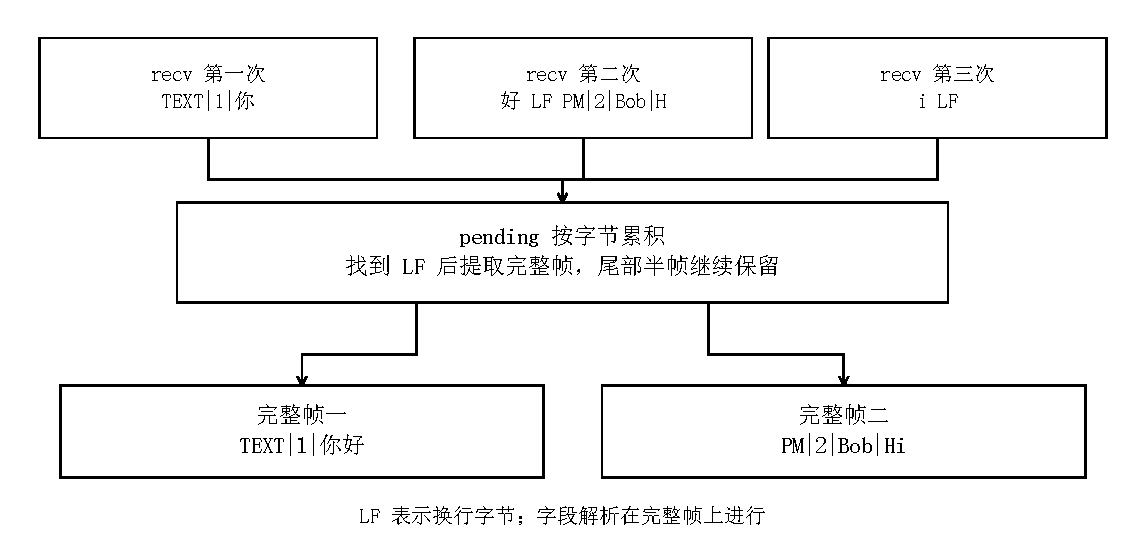
\includegraphics[width=\linewidth,height=13.5cm,keepaspectratio]{images/framing.pdf}
\captionof{figure}{接收缓存按 LF 提取完整消息的过程}\label{fig:framing}
\end{minipage}\par\smallskip
如图，第一次收到 TEXT 的前半段，第二次收全 TEXT，同时收到 PM 的开头，此时先取出 TEXT，保留 PM 的已有字节。第三次收到剩余内容后，再取出完整 PM，之后才解析其中的文字。

发送时通过 send\_frame 追加 LF，再调用 send\_all 发完全部字节；接收时循环查找 LF，分别取出同一批数据中的各条消息，并判断完整帧和剩余缓存的长度。

\subsection{登录消息}
TCP 连接建立后，先发送 JOIN|\allowbreak{}name。在服务器中判断昵称格式、重名情况和在线人数，登录成功后登记用户，返回 WELCOME|\allowbreak{}name|\allowbreak{}time，再广播上线通知。图形端收到 WELCOME 后更新登录状态，并请求在线名单和群列表。

建立 TCP 连接后仍需完成登录，才能发送聊天消息。昵称格式错误、重名或人数达到上限时返回 ERR，客户端据此在底部显示原因。

\par\medskip\noindent\begin{minipage}{\linewidth}\centering
\begin{tabular}{@{}>{\raggedright\arraybackslash}p{0.113\linewidth}>{\raggedright\arraybackslash}p{0.403\linewidth}>{\raggedright\arraybackslash}p{0.422\linewidth}@{}}
\toprule
方向 & 格式 & 语义\\
\midrule
C->S & JOIN|\allowbreak{}name & 申请使用昵称登录\\
S->C & WELCOME|\allowbreak{}name|\allowbreak{}time & 登录成功\\
C->S & WHO & 请求在线用户名单\\
S->C & USERS|\allowbreak{}name1,name2,... & 返回当前在线名单\\
S->C & NOTICE|\allowbreak{}time|\allowbreak{}text & 广播上线或离线事件\\
\bottomrule
\end{tabular}
\captionof{table}{登录和名单消息}
\end{minipage}\par\medskip
\subsection{会话状态}
\par\medskip\noindent\begin{minipage}{\linewidth}\centering
\begin{tabular}{@{}>{\raggedright\arraybackslash}p{0.159\linewidth}>{\raggedright\arraybackslash}p{0.319\linewidth}>{\raggedright\arraybackslash}p{0.460\linewidth}@{}}
\toprule
状态 & 触发事件 & 处理结果\\
\midrule
待登录 & 收到合法 JOIN & 登记昵称，发送 WELCOME，进入已登录状态\\
待登录 & 收到聊天或群组请求 & 回复 NOT\_JOINED，保留连接\\
已登录 & 收到 TEXT、PM、GTEXT & 检查序号和正文，执行相应转发\\
已登录 & 收到 GROUP 或 WHO & 处理成员操作或返回在线名单\\
已登录 & 收到 QUIT & 发送 BYE，结束工作循环并清理会话\\
任意连接状态 & recv 返回 0 或负值 & 结束工作循环，释放该连接的资源\\
\bottomrule
\end{tabular}
\captionof{table}{应用会话状态}
\end{minipage}\par\medskip
使用 Session 保存每条连接的状态，新连接的 joined 初值为 false。登录成功后登记昵称，将连接加入 online\_users，并把 joined 设为 true；连接结束时移除在线记录和群成员记录。

在图形端使用 connected 记录 TCP 连接状态，使用 joined 记录登录状态。连接成功后启动接收线程，收到 WELCOME 后启用聊天控件；重新连接时重新登录，序号从 1 开始，在线名单、群列表和收发计数随之更新。

\subsection{公共消息}
采用 TEXT|\allowbreak{}seq|\allowbreak{}content 格式发送，先校验序号和正文，再添加服务器时间，组成 MSG|\allowbreak{}time|\allowbreak{}name|\allowbreak{}seq|\allowbreak{}content，转发给全部在线用户，包括发送者本人。

收到服务器回显后，再在发送者窗口中显示这条消息。发送成功时将序号加入待回显集合，收到本人的 MSG 后移除对应序号，再增加回显计数。

\subsection{私聊消息}
采用 PM|\allowbreak{}seq|\allowbreak{}user|\allowbreak{}content 格式发送，其中 user 填写目标昵称。在在线表中找到目标连接后，添加时间和双方昵称，组成 PM|\allowbreak{}time|\allowbreak{}sender|\allowbreak{}target|\allowbreak{}seq|\allowbreak{}content，分别发给发送者和目标用户；发给本人时只回显一份。

在客户端按联系人保存记录，发出的消息存入目标用户的会话，收到的消息存入发送者的会话。切换左侧联系人后，右侧显示该联系人的聊天历史，公共消息和群消息另行保存。

\par\smallskip\noindent\begin{minipage}{\linewidth}\centering
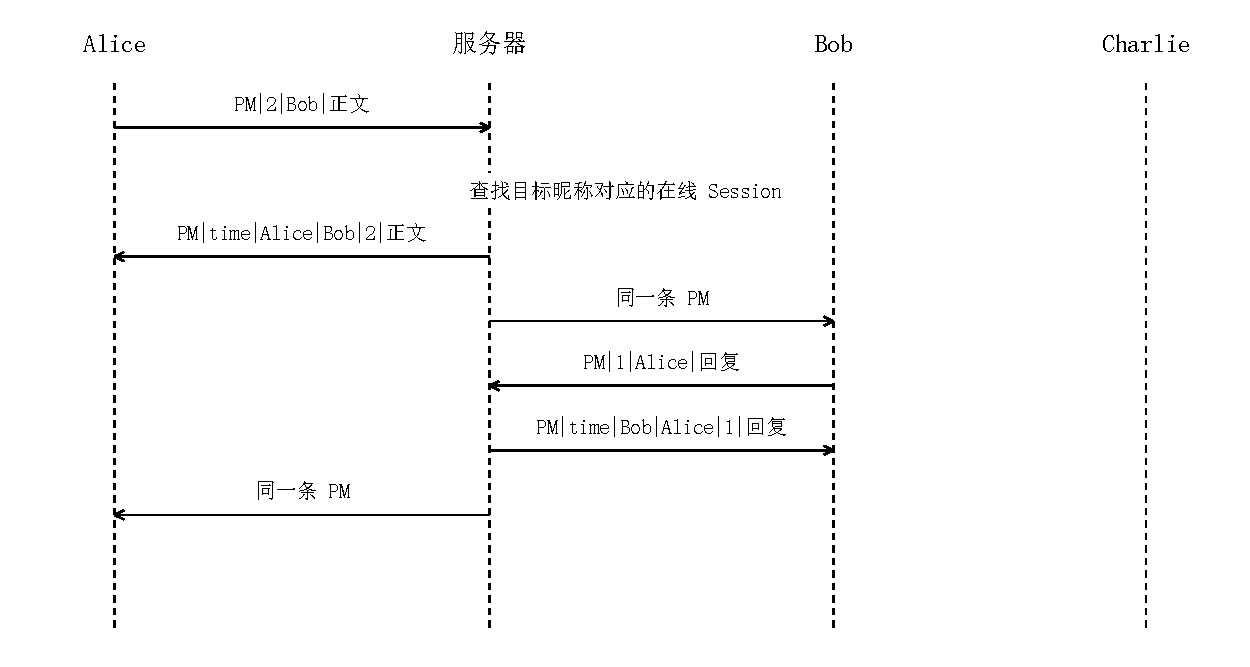
\includegraphics[width=\linewidth,height=13.5cm,keepaspectratio]{images/private_sequence.pdf}
\captionof{figure}{Alice 和 Bob 的私聊请求及服务器转发}\label{fig:private_sequence}
\end{minipage}\par\smallskip
如图，Alice 将目标填写为 Bob，服务器向两端转发相同内容。在 Alice 中保存到 Bob 会话，在 Bob 中保存到 Alice 会话，切换页面后仍能读到这段对话。

\subsection{群组消息}
使用 GROUP 创建群、添加成员、入群、退群和查询群列表，使用 GTEXT 发送聊天正文。在服务器中按群名保存成员集合，创建时加入创建者，添加成员时判断操作者的成员身份和目标在线状态，再将目标昵称加入集合。

退群时从成员集合中移除昵称，最后一位成员离开后删除空群。断开连接时也会清理群成员记录，重新登录后需要再次入群。

\begin{longtable}{@{}>{\raggedright\arraybackslash}p{0.531\linewidth}>{\raggedright\arraybackslash}p{0.434\linewidth}@{}}
\toprule
请求格式 & 处理结果\\
\midrule\endfirsthead
\toprule
请求格式 & 处理结果\\
\midrule\endhead
GROUP|\allowbreak{}CREATE|\allowbreak{}group & 建立群组，并加入创建者\\
GROUP|\allowbreak{}ADD|\allowbreak{}group|\allowbreak{}user & 将选中的在线用户加入群\\
GROUP|\allowbreak{}JOIN|\allowbreak{}group & 当前用户加入已有群\\
GROUP|\allowbreak{}LEAVE|\allowbreak{}group & 当前用户退出群\\
GROUP|\allowbreak{}LIST & 返回当前群名列表\\
GROUPS|\allowbreak{}group1,group2,... & 返回现存群名，以逗号分隔\\
GROUP\_OK|\allowbreak{}action|\allowbreak{}group & 返回建群、入群或退群成功\\
GROUP\_OK|\allowbreak{}ADD|\allowbreak{}group|\allowbreak{}user & 返回添加成员成功\\
GNOTICE|\allowbreak{}time|\allowbreak{}group|\allowbreak{}text & 通知群成员变化\\
GTEXT|\allowbreak{}seq|\allowbreak{}group|\allowbreak{}content & 客户端发送群消息\\
GMSG|\allowbreak{}time|\allowbreak{}group|\allowbreak{}sender|\allowbreak{}seq|\allowbreak{}content & 服务器向当前群成员转发\\*
\bottomrule
\caption{群组操作}\\
\end{longtable}
采用 GTEXT|\allowbreak{}seq|\allowbreak{}group|\allowbreak{}content 格式发送，校验序号、正文和群成员身份后，组成 GMSG，转发给该群的在线成员。退群后继续发送会收到 NOT\_MEMBER，对应现象在后面的测试中展示。

\par\smallskip\noindent\begin{minipage}{\linewidth}\centering
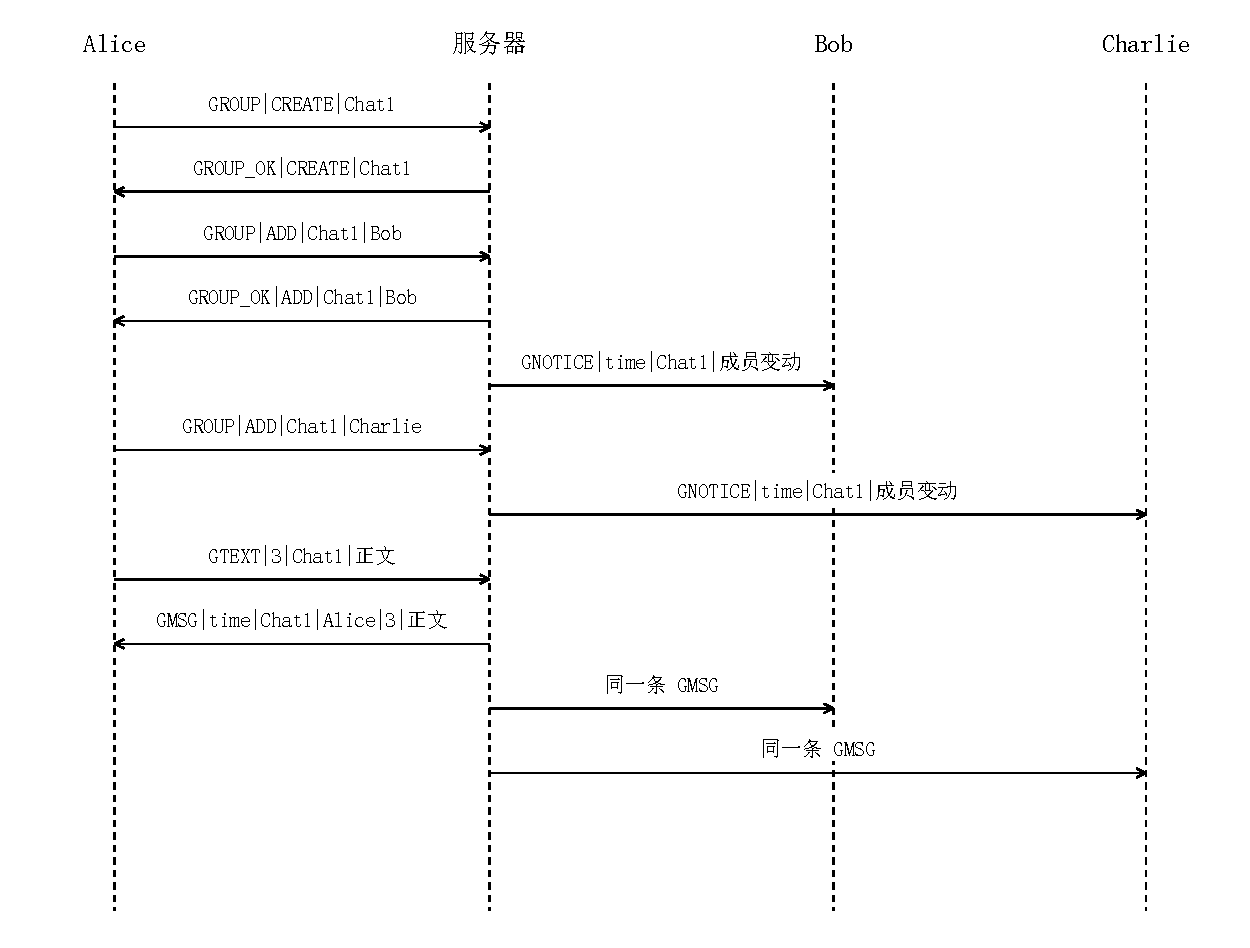
\includegraphics[width=\linewidth,height=13.5cm,keepaspectratio]{images/group_sequence.pdf}
\captionof{figure}{建群 添加成员 群发的主要交互}\label{fig:group_sequence}
\end{minipage}\par\smallskip
如图，先创建 Chat1，再添加 Bob、Charlie，最后发送群消息。操作成功后，向操作端返回 GROUP\_OK，向相关成员发送 GNOTICE；转发正文时通过 GMSG 携带群名，各客户端据此保存到 Chat1 会话。

通过 GROUPS 返回现存群名，发送群消息时再按成员集合判断身份，所以能在列表中看到群名，也需要加入该群后才能发言。

\subsection{序号规则}
从 1 开始为每条连接的聊天消息编号，TEXT、PM、GTEXT 共用同一个递增序列，GROUP 和名单查询按消息类型另行处理。收到聊天消息后，先读取 seq，同 Session 中的 next\_seq 比较，相等时才继续处理。

接受序号后先将 next\_seq 加 1，再校验正文和转发条件。因此正文超长、目标离线或群成员身份错误时，后续消息仍使用下一个序号；跳号或序号格式错误时返回 BAD\_SEQ，继续等待原序号。

这里按聊天消息编号，TCP 则按传输字节编号。例如 TEXT|\allowbreak{}1|\allowbreak{}正文 中的 1 表示第一条聊天消息，Wireshark 中的 Seq、Ack 表示字节位置，分别用于分析应用消息和 TCP 传输过程。

\subsection{时间戳}
调用 local\_timestamp 获取服务器时间，按 YYYY-MM-DD HH:MM:SS 格式写入 MSG、PM 和 GMSG，再将完整消息转发给接收者，因此各窗口显示相同的时间和正文。

精度设为秒，同一秒内可能出现多条发言，分析时结合发送者和应用序号区分。对应抓包记录时，再按流编号、方向和正文找到相应的数据。

\subsection{错误消息}
采用 ERR|\allowbreak{}code|\allowbreak{}reason 格式返回错误，其中 code 表示类别，reason 给出原因。收到完整帧后先校验 UTF-8 和登录状态，再处理字段、序号、正文及目标，客户端收到 ERR 后在底部显示提示。

\begin{longtable}{@{}>{\raggedright\arraybackslash}p{0.415\linewidth}>{\raggedright\arraybackslash}p{0.550\linewidth}@{}}
\toprule
错误码 & 触发情况\\
\midrule\endfirsthead
\toprule
错误码 & 触发情况\\
\midrule\endhead
BAD\_NAME / DUP\_NAME & 昵称格式错误或已经在线\\
NOT\_JOINED / ALREADY\_JOINED & 登录状态和请求不匹配\\
BAD\_SEQ & 应用序号格式错误或跳号\\
BAD\_TEXT / BAD\_UTF8 / TOO\_LONG & 正文、编码或长度校验失败\\
NO\_USER & 指定目标用户已离线或不存在\\
NO\_GROUP / GROUP\_EXISTS & 群不存在或群名重复\\
NOT\_MEMBER / ALREADY\_MEMBER & 群成员身份和请求不匹配\\
BAD\_FORMAT & 消息类型或字段格式错误\\
BUSY & 活动连接达到 64 条\\
FULL & 在线用户达到 32 人\\
GROUP\_FULL & 群组数量达到 32 个\\*
\bottomrule
\caption{错误响应}\\
\end{longtable}
活动连接最多为 64 条，在线用户和群组分别最多为 32 个。在接收连接、登记用户和创建群时判断数量，达到上限后分别返回 BUSY、FULL、GROUP\_FULL，其中活动连接包含尚在等待登录的连接。

一般格式错误或业务错误在返回 ERR 后继续接收，超长帧则在返回错误后关闭连接。UTF-8 和字段格式错误发生在接受序号之前，正文和转发条件错误发生在之后，后续消息分别按对应规则继续编号。

\subsection{交互时序}
先通过三次握手建立 TCP 连接，再发送 JOIN、接收 WELCOME，随后进行聊天和群操作。退出时发送 QUIT，收到 BYE 后结束连接，其他在线用户同时收到离线通知，完整顺序如下图所示。

\par\smallskip\noindent\begin{minipage}{\linewidth}\centering
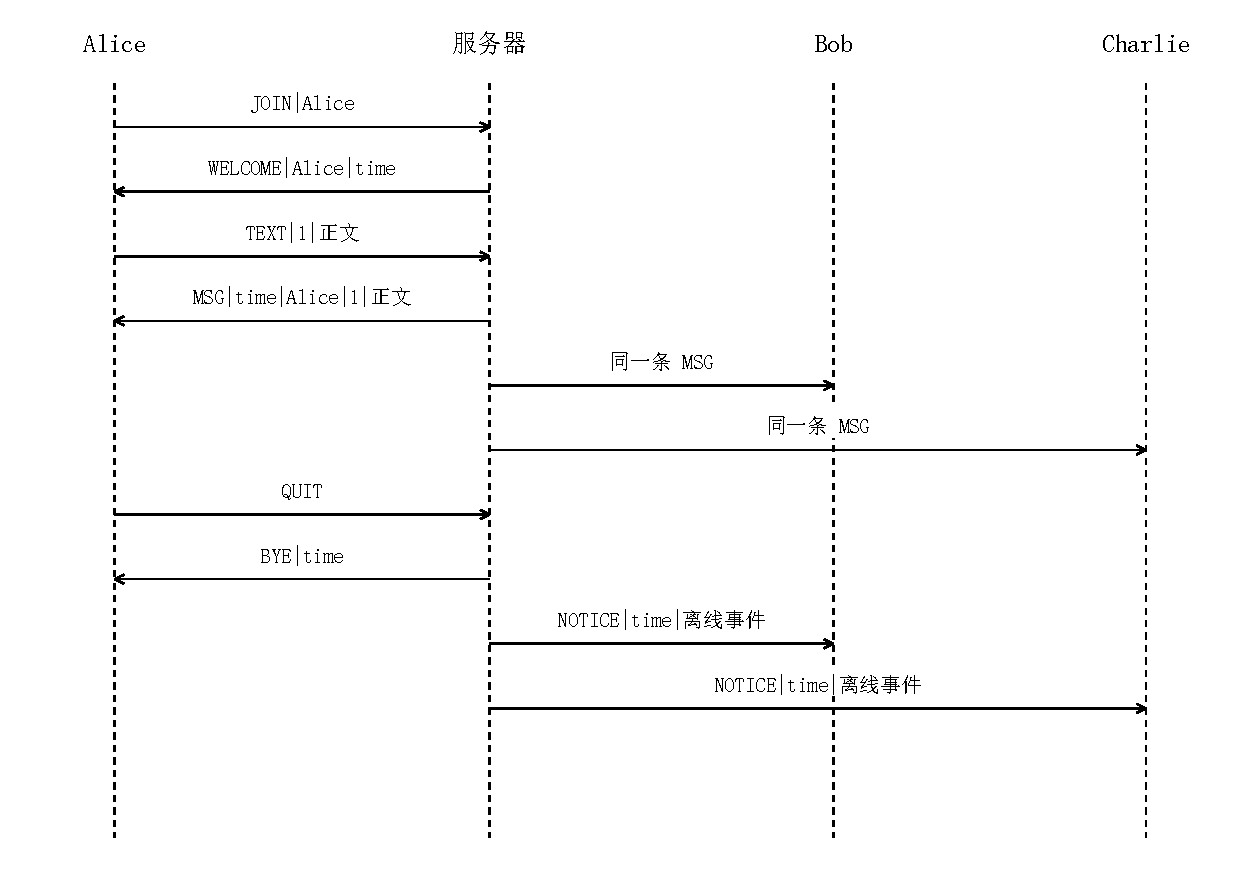
\includegraphics[width=\linewidth,height=13.5cm,keepaspectratio]{images/sequence.pdf}
\captionof{figure}{登录 聊天 退出的应用层交互顺序}\label{fig:sequence}
\end{minipage}\par\smallskip
收到本人消息的回显，表示服务器已经处理并转发这条消息；收到 TCP ACK，表示相应字节已到达对端 TCP 协议栈。因此通过界面的待回显计数观察聊天消息的处理情况，通过 Wireshark 中的序列号、确认号和分析标记观察 TCP 传输过程。

\Needspace{10\baselineskip}
\section{程序设计}
\subsection{总体架构}
采用 C/S 架构，将在线用户登记、群成员管理和消息转发集中在服务器中，客户端完成输入、协议请求生成和聊天显示。运行时先启动服务器，各客户端再分别连接并登录，消息都经服务器送达相应会话，整体关系如图所示。

在同一台电脑上运行三个客户端时，仍分别创建独立进程和套接字，以不同临时端口连接服务器的 8888 端口。在传输层通过地址、端口区分连接，在应用层再通过昵称区分聊天身份。

\par\smallskip\noindent\begin{minipage}{\linewidth}\centering
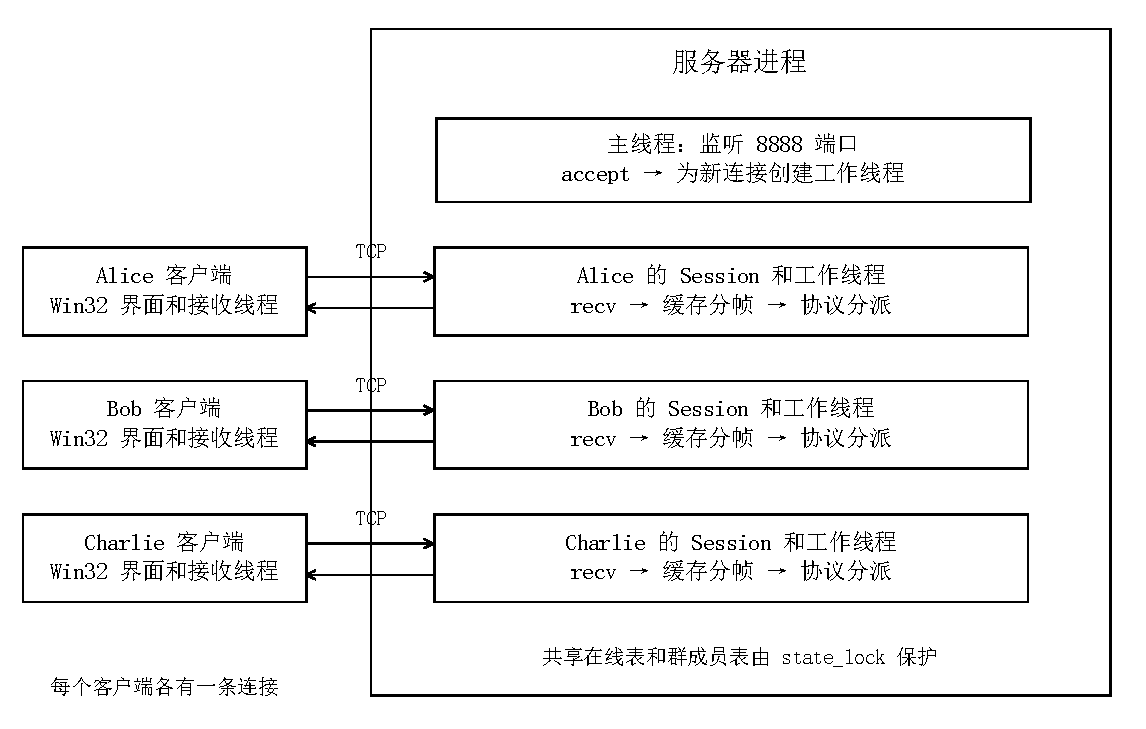
\includegraphics[width=\linewidth,height=13.5cm,keepaspectratio]{images/architecture.pdf}
\captionof{figure}{客户端服务器架构和服务器内部处理模块}\label{fig:architecture}
\end{minipage}\par\smallskip
\subsection{模块划分}
\par\medskip\noindent\begin{minipage}{\linewidth}\centering
\begin{tabular}{@{}>{\raggedright\arraybackslash}p{0.159\linewidth}>{\raggedright\arraybackslash}p{0.300\linewidth}>{\raggedright\arraybackslash}p{0.478\linewidth}@{}}
\toprule
模块 & 主要文件 & 实现内容\\
\midrule
平台适配 & net\_platform.h & 初始化 Winsock，定义句柄并关闭连接\\
协议处理 & protocol.h、protocol.cpp & 定义格式和上限，分帧、校验并发送字节\\
服务器 & server.cpp & 监听连接，登记在线用户，转发聊天并维护群成员\\
命令行客户端 & client.cpp & 读取命令，生成请求，接收并显示响应\\
图形客户端 & gui\_client.cpp & 创建窗口，选择会话，保存历史并显示动态\\
测试 & tests 目录中的 C++ 文件 & 检查协议函数、实际网络收发和窗口布局\\
\bottomrule
\end{tabular}
\captionof{table}{模块划分}
\end{minipage}\par\medskip
工程按共用网络处理、服务器业务和客户端交互划分，各模块的文件位置及功能见上表。共用函数确定字节格式和收发方式，服务器在此基础上处理聊天业务，两种客户端再将输入转成请求、将响应转成可见内容。

\subsubsection{平台适配}
将 Winsock 头文件、socket\_handle 类型和初始化、关闭函数集中在 net\_platform.h 中，其他文件经这些辅助函数完成平台相关调用，实际使用 WSAStartup、WSACleanup、closesocket 等接口。这样可以在同一位置读到平台类型及资源的建立、释放过程。

\subsubsection{协议处理}
在 protocol.h 中声明共用常量和函数，在 protocol.cpp 中处理发送、分帧、字段拆分、UTF-8、序号和时间戳。服务器、命令行端及图形端调用同一组函数，因此消息边界、编码和长度规则始终一致。

\subsubsection{服务器}
在 server.cpp 中将监听循环和连接处理分开，主线程接收连接，每条连接对应一个工作线程，再由 handle\_frame 分派登录、公聊、私聊和群操作。单条连接的数据存入 Session，在线名单和群成员集合则作为共享状态保存。

\subsubsection{命令行客户端}
命令行端从参数取得地址、端口和昵称，建连后发送 JOIN，再将键盘命令转换为应用请求；接收线程同时读取响应并打印正文及提示，使输入和收发可以持续进行。

\subsubsection{图形客户端}
图形端在 gui\_client.cpp 中创建窗口及消息回调，接收线程将完整帧经 PostMessageW 交给界面线程，再按消息类型保存历史、更新聊天区和底部动态。按钮、列表选择和窗口缩放也由界面线程处理。

\subsubsection{测试}
测试分为协议函数、真实 TCP 收发和窗口布局三类，分别写在 protocol\_tests.cpp、integration\_tests.cpp、gui\_layout\_tests.cpp 中。脚本将编译、运行及日志保存串联起来，自动化结果和后面的界面演示分别记录。

\subsection{连接状态}
以 Session 保存单条连接的状态，包括 sock、name、joined、closed 和 next\_seq，发送时通过 send\_lock 保持完整帧连续写入。连接线程和广播快照通过 shared\_ptr 引用同一会话，使发送过程能够持续访问有效句柄及状态。

\Needspace{4\baselineskip}
\VerbatimInput[fontsize=\small,breaklines=true,breakanywhere=true,numbers=left,firstnumber=1,numbersep=6pt,tabsize=4,baselinestretch=1.05]{code/listing_05.txt}
\medskip
在线表以昵称为键保存会话，群表以群名为键保存成员集合；用户登记后即可参与公聊或被选为私聊目标，连接结束时则先移除在线及群成员记录，再发送离线通知。

\subsection{服务器流程}
\par\smallskip\noindent\begin{minipage}{\linewidth}\centering
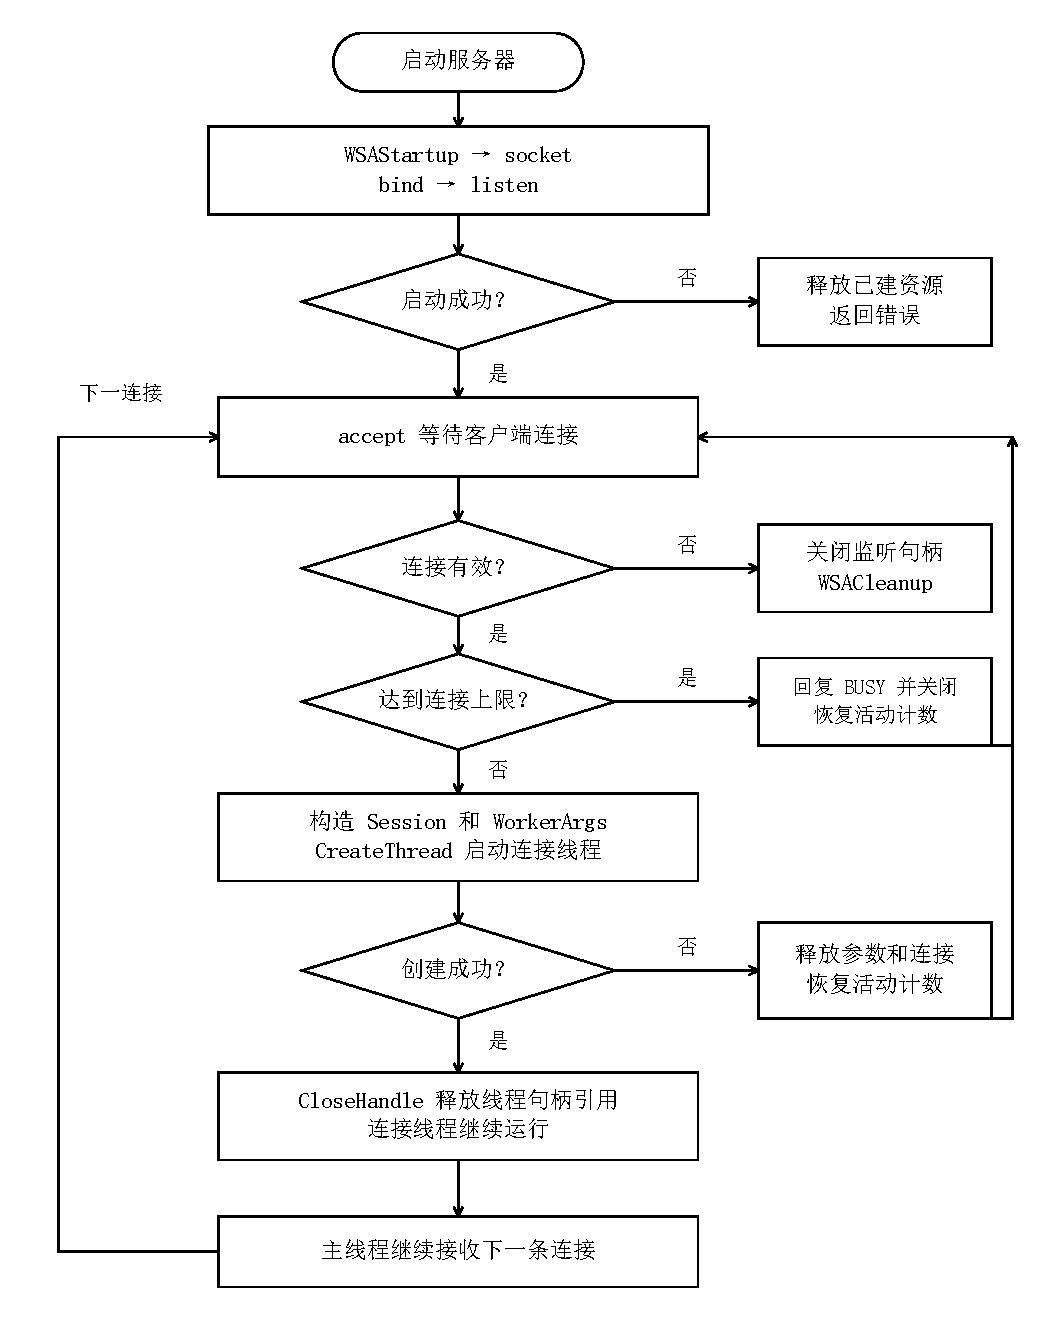
\includegraphics[width=\linewidth,height=18.7cm,keepaspectratio]{images/server_flow.pdf}
\captionof{figure}{服务器建连和单条连接的处理流程}\label{fig:server_flow}
\end{minipage}\par\smallskip
服务器在主线程中初始化 Winsock，创建监听套接字并完成 bind、listen，accept 返回通信套接字后再创建工作线程，监听循环继续接收其他连接。达到连接上限时回复 BUSY，创建线程失败时释放参数和句柄，两种情况都在清理后回到监听循环。

\par\smallskip\noindent\begin{minipage}{\linewidth}\centering
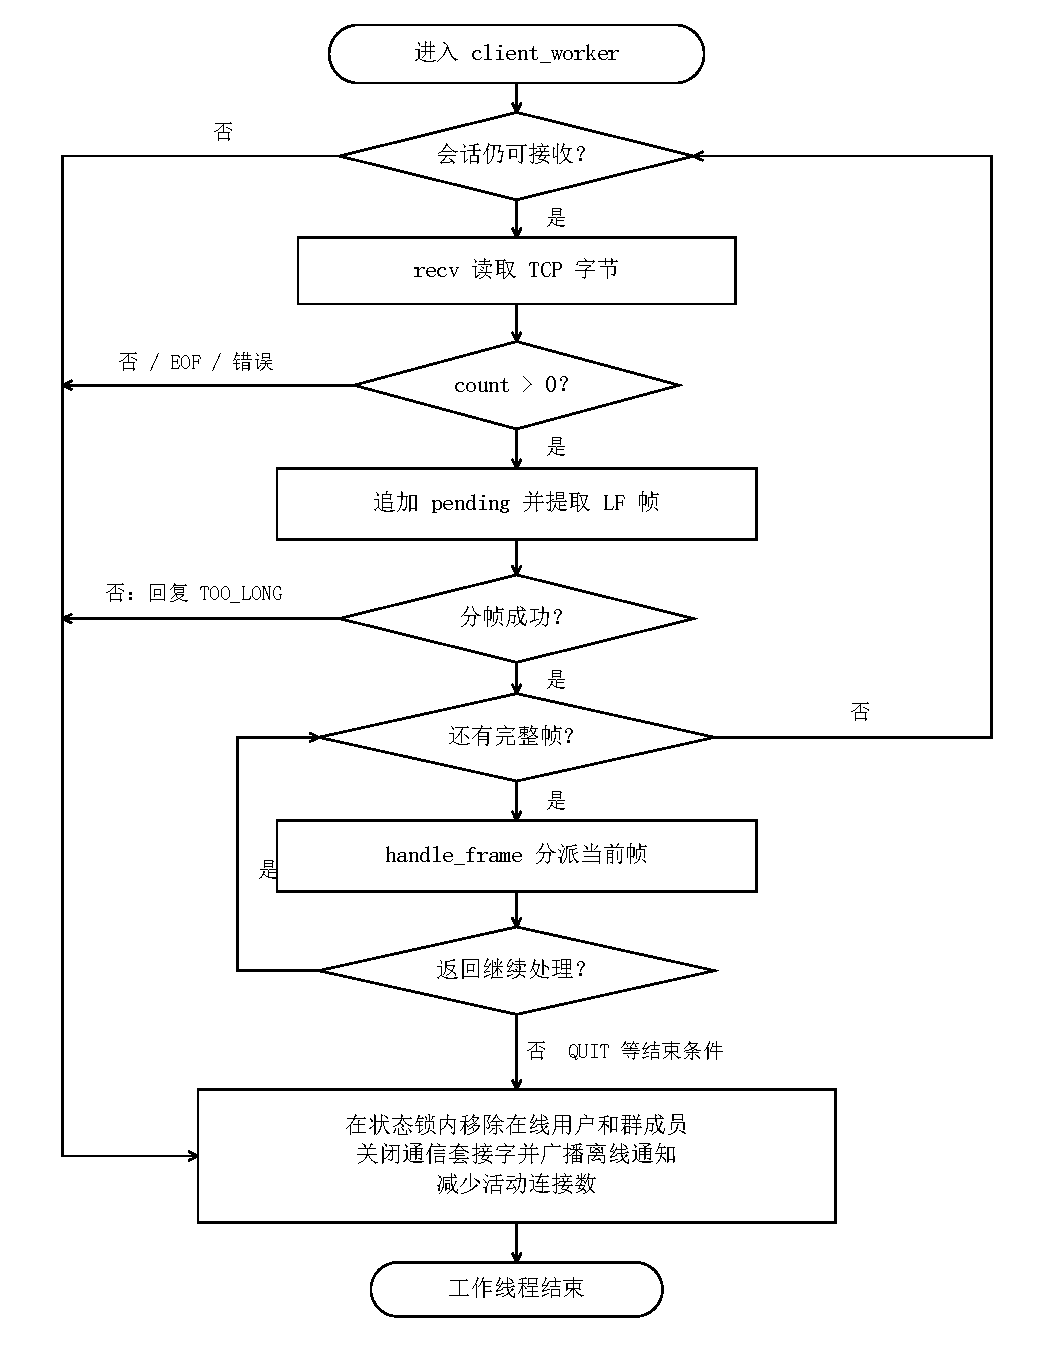
\includegraphics[width=\linewidth,height=18.7cm,keepaspectratio]{images/worker_flow.pdf}
\captionof{figure}{单条连接的接收循环及结束处理}\label{fig:worker_flow}
\end{minipage}\par\smallskip
进入 client\_worker 后持续调用 recv，将读到的字节追加到缓存，再把提取出的完整帧交给 handle\_frame。处理完当前批次后继续接收，遇到 QUIT、会话关闭、接收结束或超长帧时，再进入共同的清理路径。

普通业务处理后继续循环，已登录用户的 QUIT 则在发送 BYE 后返回 false。循环结束后，在状态锁内删除在线用户和群成员，随后关闭套接字、发送离线通知，使各类退出方式最终清理相同的数据。

\subsection{客户端流程}
\par\smallskip\noindent\begin{minipage}{\linewidth}\centering
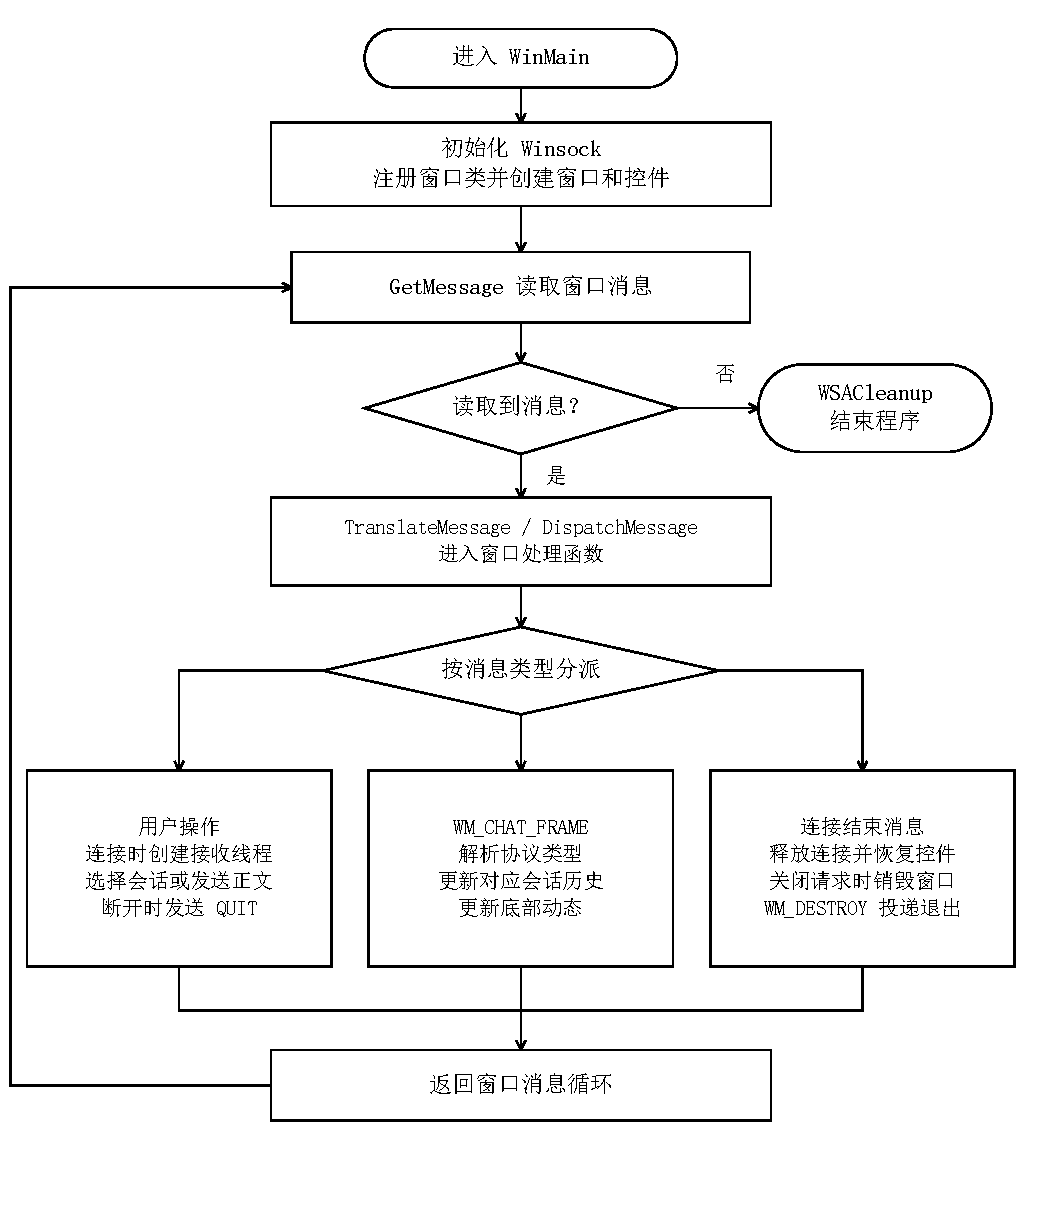
\includegraphics[width=\linewidth,height=18.7cm,keepaspectratio]{images/client_flow.pdf}
\captionof{figure}{图形客户端的发送路径和接收路径}\label{fig:client_flow}
\end{minipage}\par\smallskip
界面线程通过窗口消息循环响应操作，点击连接、发送或选择会话后进入相应处理函数；接收线程投递 WM\_CHAT\_FRAME 时，再解析完整帧、更新历史和控件。连接结束也通过消息通知界面，处理完成后继续读取下一条窗口消息。

\par\smallskip\noindent\begin{minipage}{\linewidth}\centering
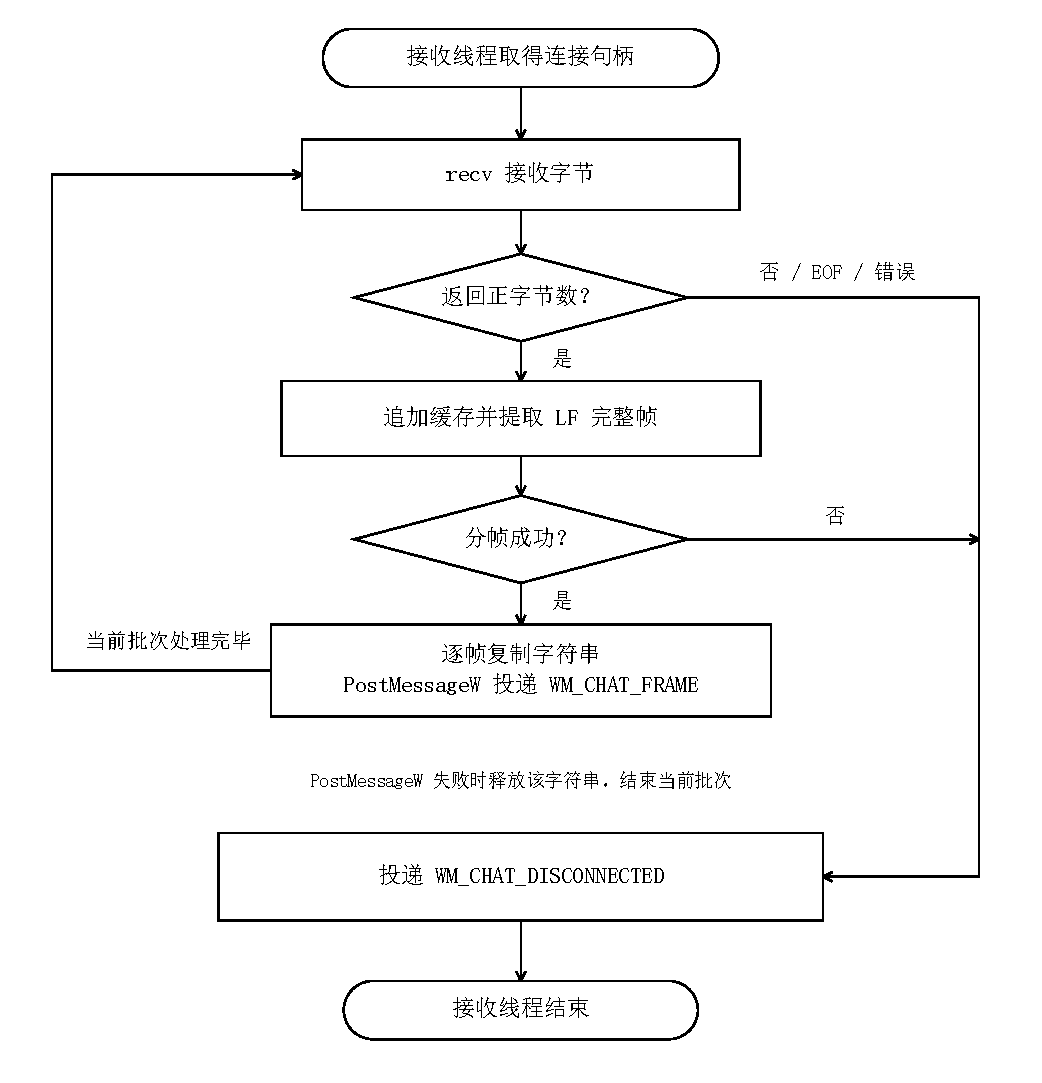
\includegraphics[width=\linewidth,height=13.5cm,keepaspectratio]{images/receive_flow.pdf}
\captionof{figure}{图形客户端接收线程的循环}\label{fig:receive_flow}
\end{minipage}\par\smallskip
连接成功后创建接收线程，循环读取通信套接字中的字节，完成分帧后将完整消息逐条投递给界面。这样，持续接收和窗口操作可以分别进行，接收结束或分帧失败时再通知界面恢复连接控件。

界面顶部放置连接参数，左侧列出公共会话、私聊联系人和群组，右侧呈现当前会话，输入框和发送按钮紧接聊天记录。底部单独记录上线、离线、成员变动、收发序号及错误提示，因此切换聊天对象时仍能连续看到连接动态。

\subsection{基本函数调用}
\par\medskip\noindent\begin{minipage}{\linewidth}\centering
\begin{tabular}{@{}>{\raggedright\arraybackslash}p{0.281\linewidth}>{\raggedright\arraybackslash}p{0.291\linewidth}>{\raggedright\arraybackslash}p{0.366\linewidth}@{}}
\toprule
函数 & 文件 & 作用\\
\midrule
WSAStartup / WSACleanup & net\_platform.h & 初始化和释放 Winsock\\
socket / bind / listen & server.cpp & 创建服务器监听端点\\
accept & server.cpp & 取得新的客户端通信套接字\\
socket / connect & client.cpp、gui\_client.cpp & 创建客户端连接\\
send & protocol.cpp & 逐段提交剩余字节\\
recv & server.cpp、客户端源码 & 接收字节并交给分帧函数\\
shutdown / closesocket & net\_platform.h、gui\_client.cpp & 关闭发送方向或释放连接\\
\bottomrule
\end{tabular}
\captionof{table}{网络函数在工程中的位置}
\end{minipage}\par\medskip
网络收发直接调用 Winsock2 基本函数，工程中的 send\_all、send\_frame 和 extract\_frames 分别补充循环发送、结束符添加和缓存分帧。登录、公聊、私聊及群操作写在 server.cpp 中，Session 保存连接状态，实际字节仍通过 send、recv 传送。

图形端同样使用 C++，通过 Win32 API 创建窗口和控件，在窗口消息处理中完成连接、会话选择、发送及缩放，再调用共用协议函数访问 TCP 连接。

\subsection{源码组织}
按业务命名主要处理函数，在 handle\_join 中登记登录，在 handle\_text 中广播公聊，在 handle\_private\_message 中选择私聊目标，在 handle\_group\_control 中修改群成员。共用常量及声明放在头文件中，简短中文注释放在相邻处理前，便于沿调用关系阅读。

\Needspace{4\baselineskip}
\VerbatimInput[fontsize=\small,breaklines=true,breakanywhere=true,numbers=left,firstnumber=1,numbersep=6pt,tabsize=4,baselinestretch=1.05]{code/listing_06.txt}
\medskip
\Needspace{10\baselineskip}
\section{程序实现}
\subsection{Winsock 初始化}
在 net\_platform.h 中包含 winsock2.h 和 ws2tcpip.h，通过 WSAStartup 请求 Winsock 2.2，初始化成功后才能创建套接字，结束时再调用 WSACleanup。SOCKET 在工程中命名为 socket\_handle，关闭连接时通过 close\_socket、shutdown\_socket 调用系统接口。

\Needspace{4\baselineskip}
\VerbatimInput[fontsize=\small,breaklines=true,breakanywhere=true,numbers=left,firstnumber=1,numbersep=6pt,tabsize=4,baselinestretch=1.05]{code/listing_07.txt}
\medskip
这些辅助函数集中处理平台接口，循环发送、分帧和消息分派则在工程源码中实现，从初始化到 send、recv 的调用路径可以沿文件中的函数继续阅读。[2][4]

\subsection{监听套接字}
创建监听端点时，将 AF\_INET、SOCK\_STREAM、IPPROTO\_TCP 传入 socket，随后在 sockaddr\_in 中填写 IPv4 地址和端口。端口通过 htons 转为网络字节序，地址整数通过 htonl 转换后写入结构。

\Needspace{4\baselineskip}
\VerbatimInput[fontsize=\small,breaklines=true,breakanywhere=true,numbers=left,firstnumber=1,numbersep=6pt,tabsize=4,baselinestretch=1.05]{code/listing_08.txt}
\medskip
默认地址使用 INADDR\_LOOPBACK，即 127.0.0.1，接着调用 bind 绑定本地地址、调用 listen 开始监听；任何一步返回错误，都读取错误码并释放已创建的资源。填写这些网络字段时统一进行字节序转换，使两端按相同顺序解释整数。[2]

\subsection{接收连接}
accept 返回新的通信句柄，原监听句柄继续留在循环中，remote 同时取得对端地址。通过 active\_connections 记录活动连接数，达到上限后回复 BUSY 并关闭新连接，正常连接则交给工作线程。

\Needspace{4\baselineskip}
\VerbatimInput[fontsize=\small,breaklines=true,breakanywhere=true,numbers=left,firstnumber=1,numbersep=6pt,tabsize=4,baselinestretch=1.05]{code/listing_09.txt}
\medskip
将 Session 放入 WorkerArgs，经 CreateThread 传给 worker\_entry，再在线程入口调用 client\_worker。主线程随后 CloseHandle，释放自己持有的线程句柄引用，工作线程则继续处理该连接，因此能够同时接收其他用户。

\subsection{客户端连接}
图形端从输入框取得地址和端口，分别通过 inet\_pton、htons 转换，再创建套接字并调用 connect。建连成功后发送 JOIN，失败时释放句柄并在底部显示原因，连接处理如下。

\Needspace{4\baselineskip}
\VerbatimInput[fontsize=\small,breaklines=true,breakanywhere=true,numbers=left,firstnumber=1,numbersep=6pt,tabsize=4,baselinestretch=1.05]{code/listing_10.txt}
\medskip
登录结果在接收路径中返回，收到 WELCOME 后更新昵称、窗口标题和按钮，再请求在线名单，由此将网络建连和应用登录衔接起来。

\subsection{循环发送}
send 的返回值是实际提交的字节数，因此使用 sent 保存累计长度，每轮从尚未发送的位置继续提交。返回正数时推进指针，返回零或错误时结束发送，直到全部字节处理完毕才返回成功。

\Needspace{4\baselineskip}
\VerbatimInput[fontsize=\small,breaklines=true,breakanywhere=true,numbers=left,firstnumber=1,numbersep=6pt,tabsize=4,baselinestretch=1.05]{code/listing_11.txt}
\medskip
一帧可能经过多次 send，接收端也可能经过多次 recv 才读全，所以循环发送和缓存分帧需要配合使用；两处都按字节计算长度，中文编码也随原字节保留。

send\_frame 先判断长度及结束符，再复制内容、追加 LF 并调用 send\_all。登录、聊天和群请求都由这一入口发送，拥有相同的边界格式；本地提交成功后，仍需等待服务器回显才能得到应用处理结果。

\Needspace{4\baselineskip}
\VerbatimInput[fontsize=\small,breaklines=true,breakanywhere=true,numbers=left,firstnumber=1,numbersep=6pt,tabsize=4,baselinestretch=1.05]{code/listing_12.txt}
\medskip
\subsection{接收分帧}
recv 每次读入的 count 个字节都追加到 pending，随后循环寻找 LF，把之前的内容保存为完整帧并移除已处理前缀。多帧可以在同一轮分别取出，末尾半帧则继续保留，接收缓存的实现如下。

\Needspace{4\baselineskip}
\VerbatimInput[fontsize=\small,breaklines=true,breakanywhere=true,numbers=left,firstnumber=1,numbersep=6pt,tabsize=4,baselinestretch=1.05]{code/listing_13.txt}
\medskip
例如读到 TEXT|\allowbreak{}1|\allowbreak{} 时暂存字节，下一批补齐正文和 LF 后才能交给业务函数；一次读到两条完整消息时，就依次提取两帧。完整帧和剩余缓存分别判断长度，超长时结束接收。

TEXT 最多拆分两次，PM、GTEXT 最多拆分三次，再将剩余部分保留为正文，因此“你好 Bob! Hello|\allowbreak{}世界”中的竖线仍能作为聊天内容传送。

\Needspace{4\baselineskip}
\VerbatimInput[fontsize=\small,breaklines=true,breakanywhere=true,numbers=left,firstnumber=1,numbersep=6pt,tabsize=4,baselinestretch=1.05]{code/listing_14.txt}
\medskip
\subsection{消息序号校验}
序号解析逐位读取十进制数字，在乘以 10 前判断是否超出 uint64\_t 范围，再与 next\_seq 比较。网络测试中先发送 999，得到 BAD\_SEQ 后使用原期待值继续发送，随后收到了正常广播。

\Needspace{4\baselineskip}
\VerbatimInput[fontsize=\small,breaklines=true,breakanywhere=true,numbers=left,firstnumber=1,numbersep=6pt,tabsize=4,baselinestretch=1.05]{code/listing_15.txt}
\medskip
\subsection{中文编码}
Win32 宽字符接口处理 UTF-16，网络传输统一采用 UTF-8，所以发送前先计算转换长度并分配字符串，接收完整帧后再转换回宽字符，通过 SetWindowTextW 等接口显示。

\Needspace{4\baselineskip}
\VerbatimInput[fontsize=\small,breaklines=true,breakanywhere=true,numbers=left,firstnumber=1,numbersep=6pt,tabsize=4,baselinestretch=1.05]{code/listing_16.txt}
\medskip
\Needspace{4\baselineskip}
\VerbatimInput[fontsize=\small,breaklines=true,breakanywhere=true,numbers=left,firstnumber=1,numbersep=6pt,tabsize=4,baselinestretch=1.05]{code/listing_17.txt}
\medskip
缓存阶段始终保留原字节，完整帧形成后才处理 UTF-8；即使一个汉字跨多批到达，也能在拼接后得到完整编码。正文同时经过空文本、长度和控制字符判断，后面的中英文界面记录呈现了实际显示结果。

\subsection{公共广播}
在 handle\_text 中取得序号和正文，接受序号后增加 next\_seq，再判断正文并生成服务器时间，最后组成 MSG、调用 broadcast，同时记录发送者和序号。

\Needspace{4\baselineskip}
\VerbatimInput[fontsize=\small,breaklines=true,breakanywhere=true,numbers=left,firstnumber=1,numbersep=6pt,tabsize=4,baselinestretch=1.05]{code/listing_18.txt}
\medskip
广播时先在状态锁内复制在线会话，释放状态锁后再向各连接发送，因此访问共享名单的临界区较短，实际发送则由每条连接自己的发送锁保护。

\Needspace{4\baselineskip}
\VerbatimInput[fontsize=\small,breaklines=true,breakanywhere=true,numbers=left,firstnumber=1,numbersep=6pt,tabsize=4,baselinestretch=1.05]{code/listing_19.txt}
\medskip
\Needspace{4\baselineskip}
\VerbatimInput[fontsize=\small,breaklines=true,breakanywhere=true,numbers=left,firstnumber=1,numbersep=6pt,tabsize=4,baselinestretch=1.05]{code/listing_20.txt}
\medskip
\subsection{私聊转发}
私聊先按目标昵称查询在线表，再生成带时间、双方身份、序号和正文的 PM，发送给本人及目标；目标为本人时保留一份回显，相关转发过程如下。

\Needspace{4\baselineskip}
\VerbatimInput[fontsize=\small,breaklines=true,breakanywhere=true,numbers=left,firstnumber=1,numbersep=6pt,tabsize=4,baselinestretch=1.05]{code/listing_21.txt}
\medskip
接收者由服务器选定，客户端再按双方昵称保存历史。选择 Bob 时读取 Bob 私聊，切回公共聊天室时读取公共历史，后面的会话切换记录可以看到两类消息分别保留。

\subsection{群成员管理}
群名通过 map 对应到成员 set，添加时调用 insert，并通过插入结果区分是否已经加入；成员增删都在 state\_lock 内完成，随后向相应成员发送 GNOTICE。

\Needspace{4\baselineskip}
\VerbatimInput[fontsize=\small,breaklines=true,breakanywhere=true,numbers=left,firstnumber=1,numbersep=6pt,tabsize=4,baselinestretch=1.05]{code/listing_22.txt}
\medskip
在群页面中选择在线用户并添加时，每位目标对应一条 GROUP|\allowbreak{}ADD|\allowbreak{}group|\allowbreak{}user 请求，服务器据此修改集合。群列表列出现存群名，具体发言和接收范围则由成员集合决定。

在 handle\_group\_text 中完成格式、序号和正文判断后，再判断发送者是否属于该群，通过后生成 GMSG，按 group\_snapshot 返回的在线会话转发。退群删除昵称后，下一次群发就使用更新后的集合。

\Needspace{4\baselineskip}
\VerbatimInput[fontsize=\small,breaklines=true,breakanywhere=true,numbers=left,firstnumber=1,numbersep=6pt,tabsize=4,baselinestretch=1.05]{code/listing_23.txt}
\medskip
\subsection{线程同步}
Alice 和 Bob 同时发言时，两个工作线程都可能向 Charlie 转发，因此在一帧发送期间持有 Charlie 会话的 send\_lock，发完整帧后才释放，防止不同帧的字节在同一连接上交错写入。

\Needspace{4\baselineskip}
\VerbatimInput[fontsize=\small,breaklines=true,breakanywhere=true,numbers=left,firstnumber=1,numbersep=6pt,tabsize=4,baselinestretch=1.05]{code/listing_24.txt}
\medskip
共享在线表及群表使用 state\_lock，日志输出使用 output\_lock，关闭状态通过原子变量 closed 更新，分别对应名单修改、连接发送和日志记录等并发访问。

\subsection{图形接收线程}
接收线程将完整帧复制到独立字符串，通过 PostMessageW 投递 WM\_CHAT\_FRAME，界面处理完后再释放这份数据。网络接收结束时另发连接结束通知，由界面线程统一更新连接状态。

\Needspace{4\baselineskip}
\VerbatimInput[fontsize=\small,breaklines=true,breakanywhere=true,numbers=left,firstnumber=1,numbersep=6pt,tabsize=4,baselinestretch=1.05]{code/listing_25.txt}
\medskip
接收到 MSG、PM、GMSG 后，按类型追加到公共、私聊和群历史；NOTICE、GNOTICE、ERR 则追加到底部动态。两类记录分别保存，因此聊天对象变化时，连接事件仍按时间连续显示。

\Needspace{4\baselineskip}
\VerbatimInput[fontsize=\small,breaklines=true,breakanywhere=true,numbers=left,firstnumber=1,numbersep=6pt,tabsize=4,baselinestretch=1.05]{code/listing_26.txt}
\medskip
\subsection{正常退出}
点击断开后，先设置 disconnecting 并发送 QUIT，接着关闭套接字写方向，继续接收 BYE。读到连接结束后，再通知界面关闭句柄、恢复连接按钮，使退出经过完整的应用交互。

\Needspace{4\baselineskip}
\VerbatimInput[fontsize=\small,breaklines=true,breakanywhere=true,numbers=left,firstnumber=1,numbersep=6pt,tabsize=4,baselinestretch=1.05]{code/listing_27.txt}
\medskip
关闭窗口时设置 close\_pending，进入相同退出路径，收到连接结束通知后销毁窗口，等待超时则由定时器结束关闭处理。服务器收到 QUIT、EOF 或 Socket 错误后，统一清理在线及群成员数据，再向其他用户发送离线通知。

\subsection{命令行客户端}
命令行端在 client.cpp 中解析地址、端口和昵称，建立连接后发送 JOIN，主线程持续读取键盘输入，接收线程同时打印服务器消息。普通正文生成 TEXT，/pm 生成 PM，群命令生成 GROUP 或 GTEXT，/quit 则进入退出过程。

命令行端和图形端共用协议函数并连接同一服务器，区别在于请求从键盘命令还是按钮、列表生成，因此可以在两种界面中完成相同聊天操作。

\subsection{编译}
在 MSVC 开发者命令行中运行 build.bat，生成服务器、命令行端和测试程序，再运行 build\_gui.bat 生成图形端。编译时使用 /utf-8 读取中文源码，链接 Ws2\_32.lib，图形端另链接 User32.lib、Gdi32.lib。

\Needspace{4\baselineskip}
\VerbatimInput[fontsize=\small,breaklines=true,breakanywhere=true,numbers=left,firstnumber=1,numbersep=6pt,tabsize=4,baselinestretch=1.05]{code/listing_28.txt}
\medskip
编译后可在 bin 中得到 server.exe、client.exe、gui\_client.exe、protocol\_tests.exe 和 integration\_tests.exe，正式程序及测试均以 C++ 编写，PowerShell 脚本用来组织启动和保存日志。

\subsection{运行}
在 Windows PowerShell 进入工程目录后运行三窗口脚本，即可打开服务器及 Alice、Bob、Charlie 客户端，再分别点击连接服务器。关闭其中一位用户后，保持服务器运行，通过 --name 参数可以单独重新打开该客户端。

\Needspace{4\baselineskip}
\VerbatimInput[fontsize=\small,breaklines=true,breakanywhere=true,numbers=left,firstnumber=1,numbersep=6pt,tabsize=4,baselinestretch=1.05]{code/listing_29.txt}
\medskip
\Needspace{4\baselineskip}
\VerbatimInput[fontsize=\small,breaklines=true,breakanywhere=true,numbers=left,firstnumber=1,numbersep=6pt,tabsize=4,baselinestretch=1.05]{code/listing_30.txt}
\medskip
\Needspace{4\baselineskip}
\VerbatimInput[fontsize=\small,breaklines=true,breakanywhere=true,numbers=left,firstnumber=1,numbersep=6pt,tabsize=4,baselinestretch=1.05]{code/listing_31.txt}
\medskip
\par\medskip\noindent\begin{minipage}{\linewidth}\centering
\begin{tabular}{@{}>{\raggedright\arraybackslash}p{0.434\linewidth}>{\raggedright\arraybackslash}p{0.531\linewidth}@{}}
\toprule
输入 & 效果\\
\midrule
/list & 查询在线用户\\
/pm Bob 你好 & 向 Bob 私聊\\
/group create Chat1 & 建立群组\\
/group join Chat1 & 加入已有群\\
/group leave Chat1 & 退出群\\
/g Chat1 Hello & 发送群消息\\
/groups & 查询群列表\\
/quit & 退出连接\\
普通文字 & 发送公共消息\\
\bottomrule
\end{tabular}
\captionof{table}{命令行客户端操作}
\end{minipage}\par\medskip
图形端在聊天页选择用户即可进入私聊，在群组页填写群名、建立群聊并选择成员，输入正文后点击发送或按回车，底部同时显示相关操作结果。

\Needspace{10\baselineskip}
\section{功能测试}
\subsection{三人登录}
服务器启动后，依次以 Alice、Bob、Charlie 连接 127.0.0.1:8888，每登录一位用户，都能在本人窗口看到登录成功提示，在已在线窗口看到新的上线事件。以下按实际连接顺序记录页面变化。

Alice 首先登录时只有一位用户，Bob 和 Charlie 随后加入，在线人数逐次增加到 3；最后切回 Alice，可以看到后两位用户的上线记录。

\par\smallskip\noindent\begin{minipage}{\linewidth}\centering
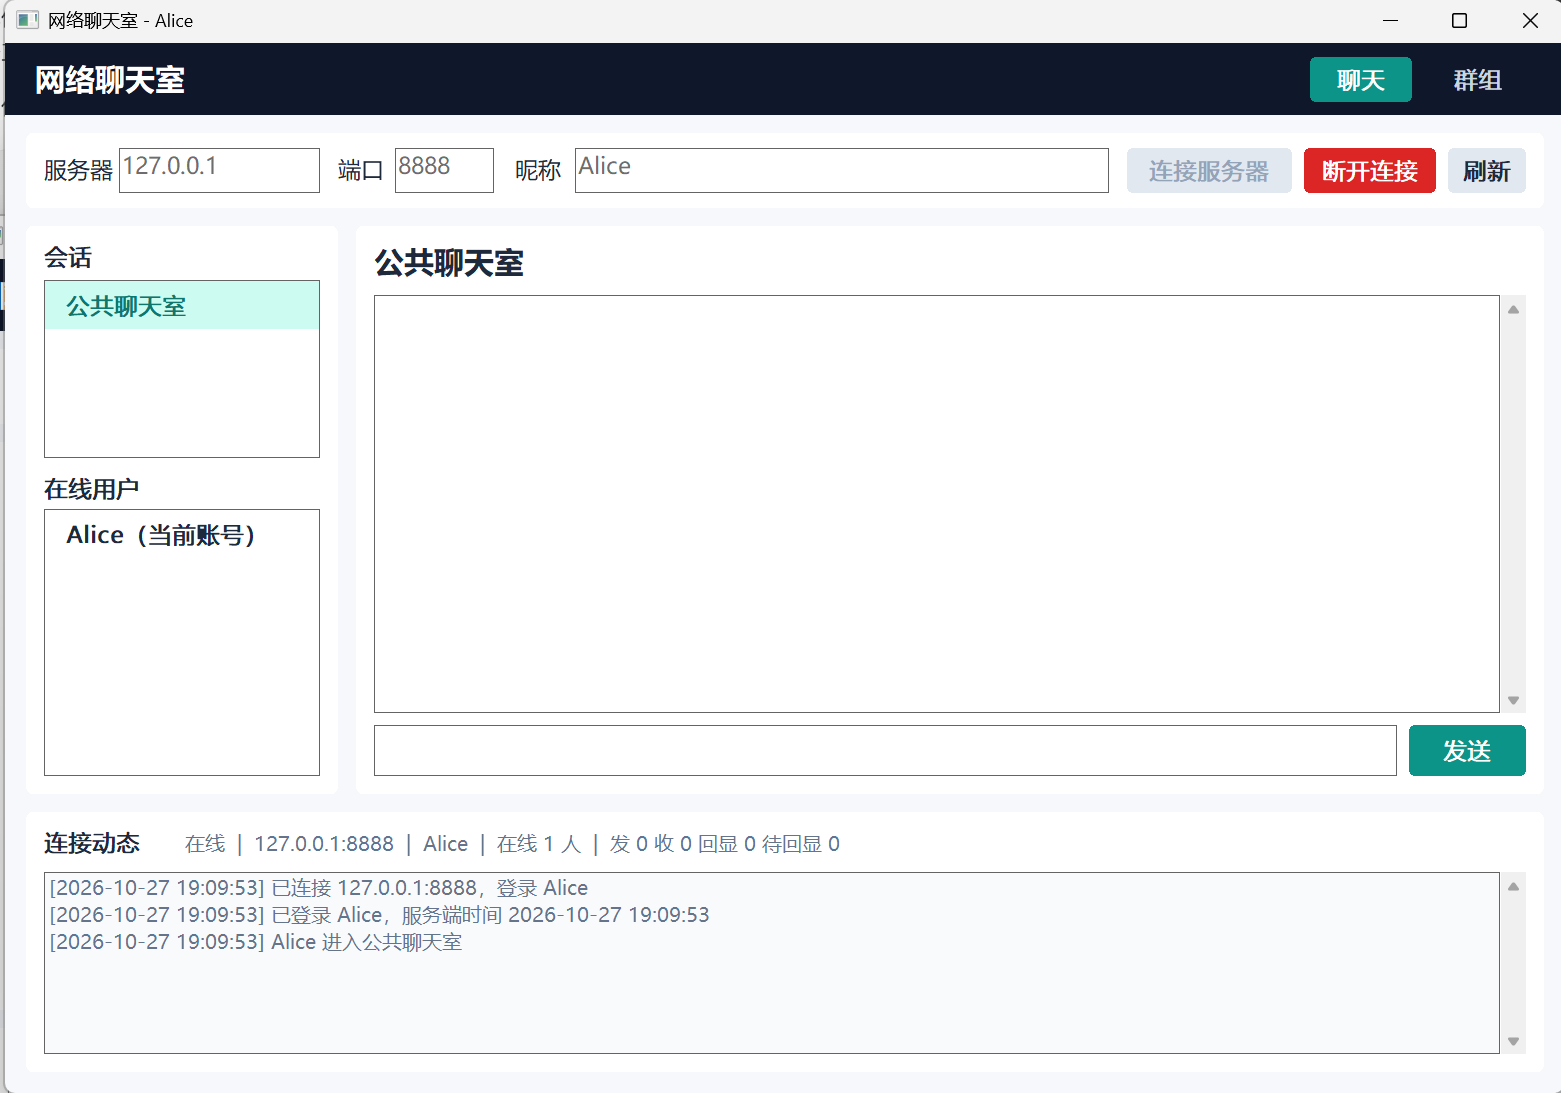
\includegraphics[width=\linewidth,height=10.0cm,keepaspectratio]{images/screen_01.png}
\captionof{figure}{Alice 登录后的界面}\label{fig:s01}
\par\smallskip{\raggedright\setlength{\parindent}{2em}\indent 输入 Alice 并连接后，可以看到登录成功提示，在线名单中只有 Alice，人数为 1。\par}
\end{minipage}\par\smallskip
\par\smallskip\noindent\begin{minipage}{\linewidth}\centering
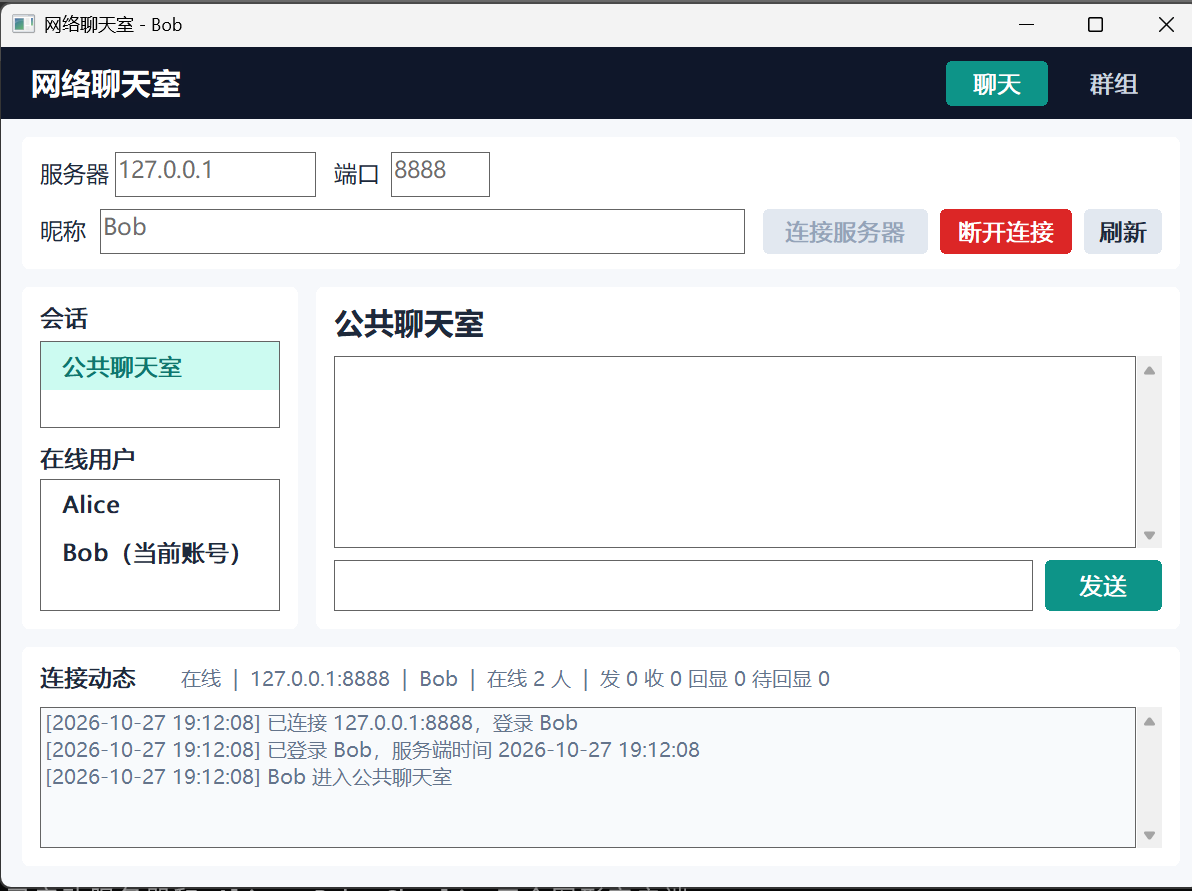
\includegraphics[width=\linewidth,height=10.0cm,keepaspectratio]{images/screen_02.png}
\captionof{figure}{Bob 登录后的界面}\label{fig:s02}
\par\smallskip{\raggedright\setlength{\parindent}{2em}\indent Bob 随后连接，名单中出现 Alice、Bob，在线人数增加到 2。\par}
\end{minipage}\par\smallskip
\par\smallskip\noindent\begin{minipage}{\linewidth}\centering
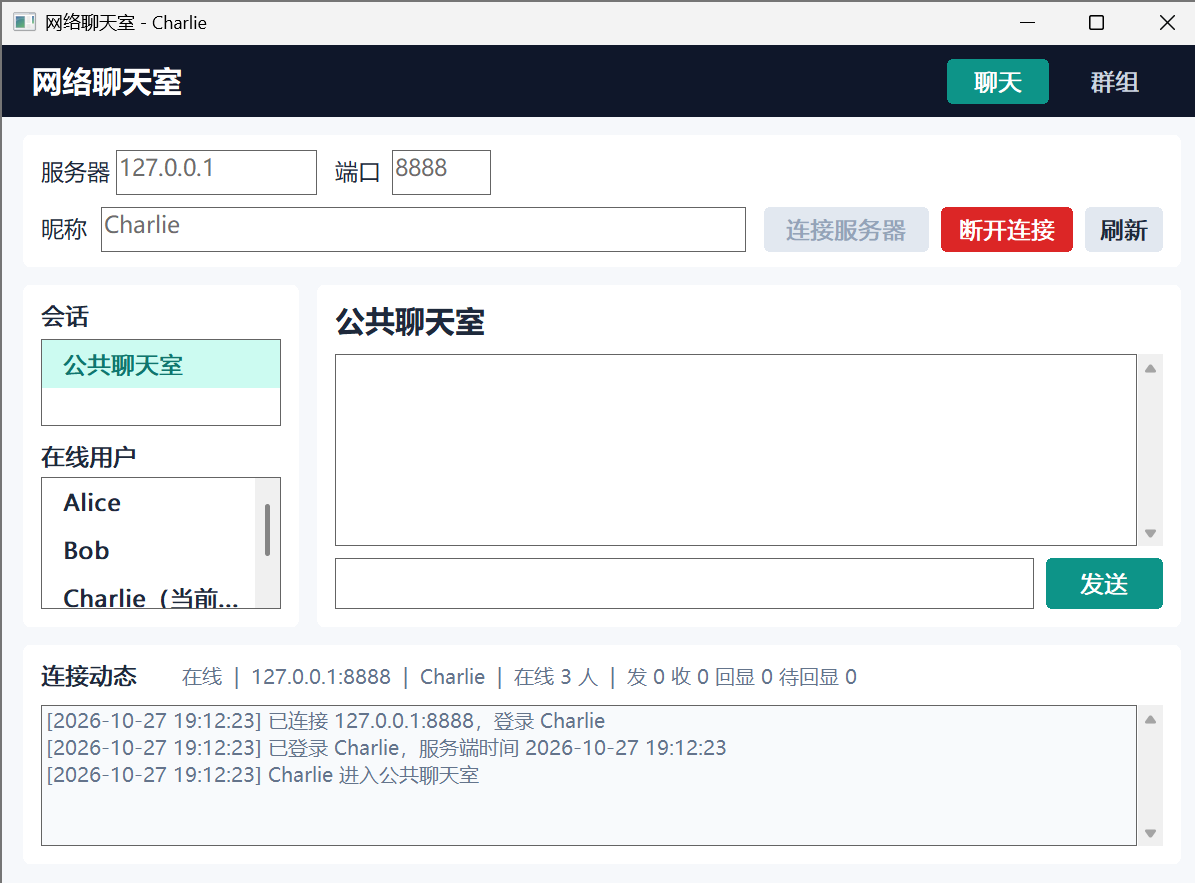
\includegraphics[width=\linewidth,height=10.0cm,keepaspectratio]{images/screen_03.png}
\captionof{figure}{Charlie 登录后的界面}\label{fig:s03}
\par\smallskip{\raggedright\setlength{\parindent}{2em}\indent Charlie 登录后，名单列出三位昵称，在线人数变为 3。\par}
\end{minipage}\par\smallskip
\par\smallskip\noindent\begin{minipage}{\linewidth}\centering
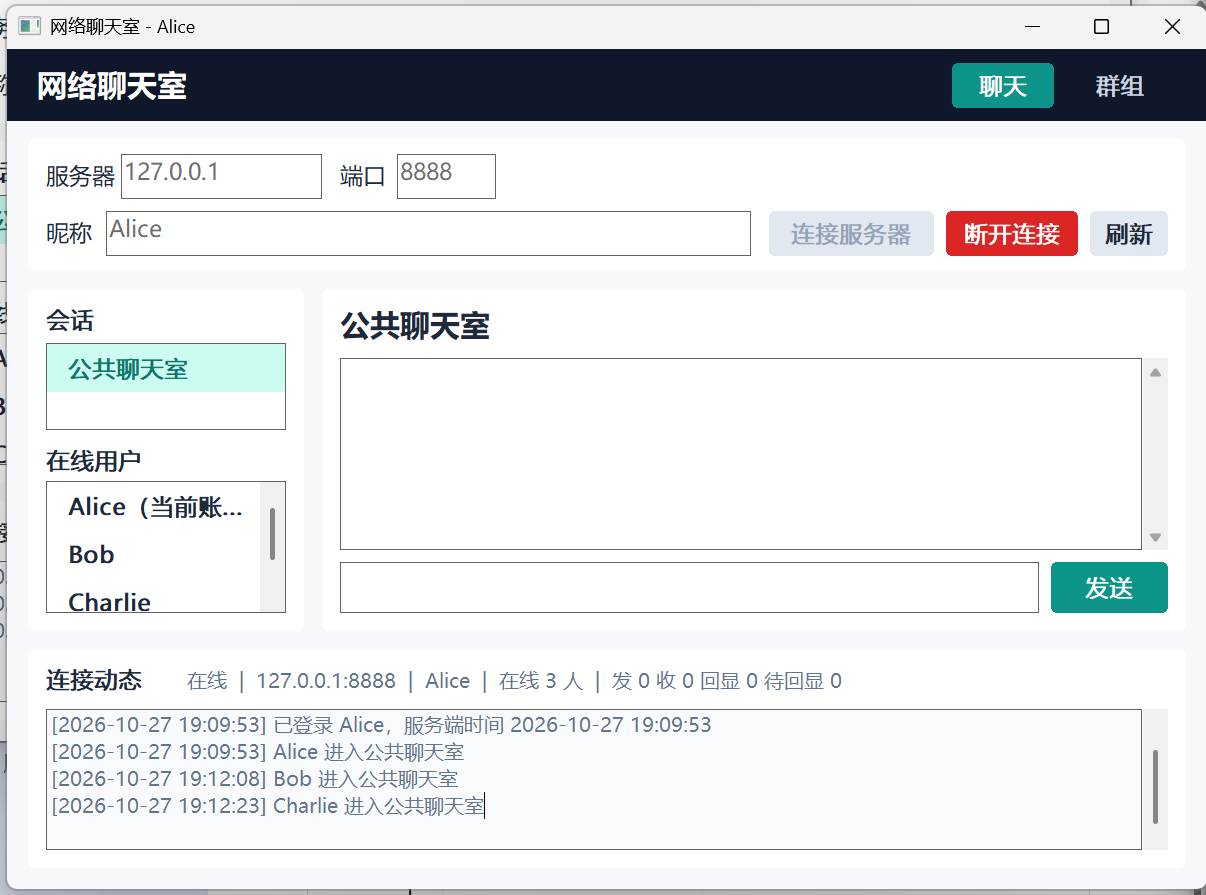
\includegraphics[width=\linewidth,height=10.0cm,keepaspectratio]{images/screen_04.png}
\captionof{figure}{Alice 收到两位用户的上线通知}\label{fig:s04}
\par\smallskip{\raggedright\setlength{\parindent}{2em}\indent 切回 Alice 后，可以看到 Bob 和 Charlie 的上线通知，已经在线的用户也收到了新连接事件。\par}
\end{minipage}\par\smallskip
三个窗口中的在线名单一致，说明三条独立连接已分别登记昵称，随后可以在这些会话中发送公共或定向消息。

\subsection{公共聊天}
三人都进入公共聊天室后，先由 Alice 发送中英文消息，再由 Bob、Charlie 依次回复，每次发言都在另外两个窗口中出现。

聊天记录中的时间、昵称和正文对应同一条转发消息，发送者底部同时出现 TEXT、MSG，接收者底部增加 MSG，由此可以看到客户端请求及服务器广播的先后过程。

\par\smallskip\noindent\begin{minipage}{\linewidth}\centering
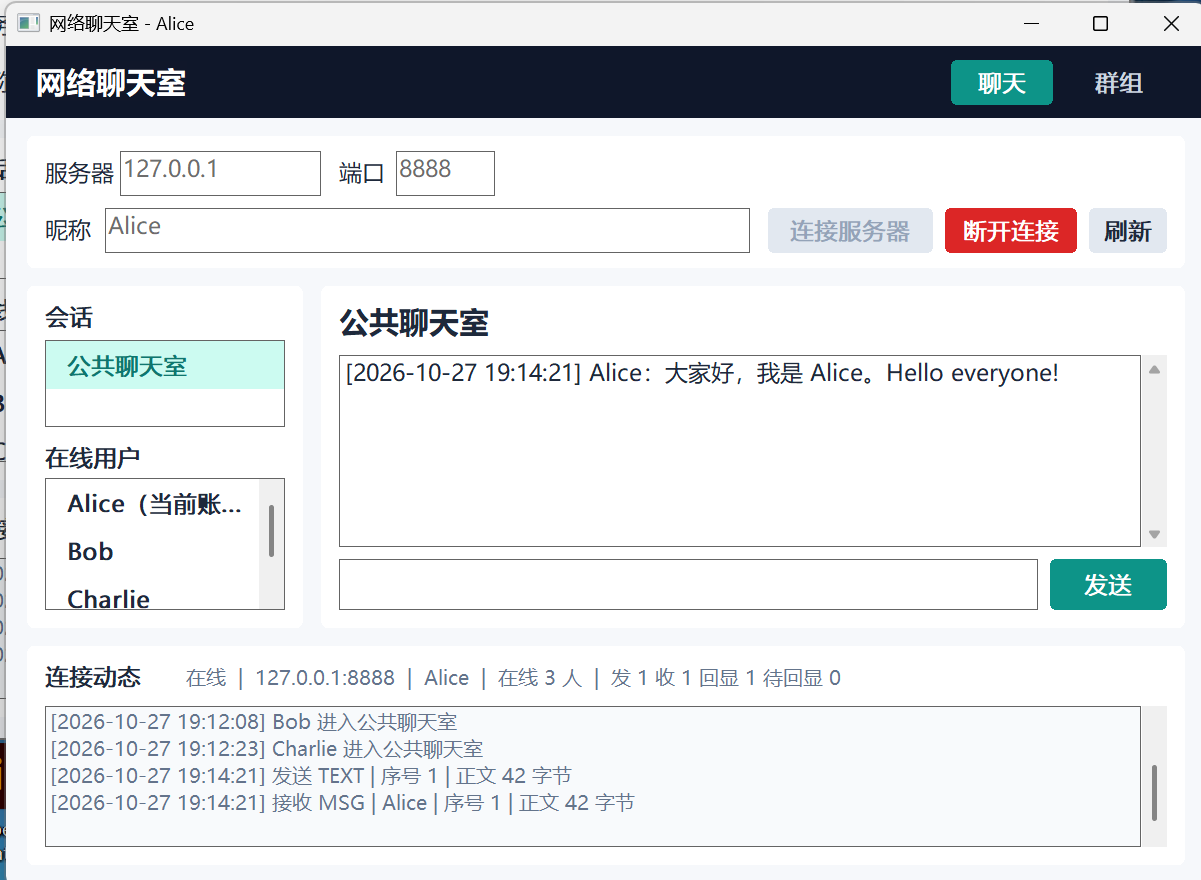
\includegraphics[width=\linewidth,height=10.0cm,keepaspectratio]{images/screen_05.png}
\captionof{figure}{Alice 的中英文公共发言}\label{fig:s05}
\par\smallskip{\raggedright\setlength{\parindent}{2em}\indent Alice 发送中英文公共消息后，聊天区出现时间、本人昵称和正文，下方同时出现 TEXT 发送及 MSG 回显。\par}
\end{minipage}\par\smallskip
\par\smallskip\noindent\begin{minipage}{\linewidth}\centering
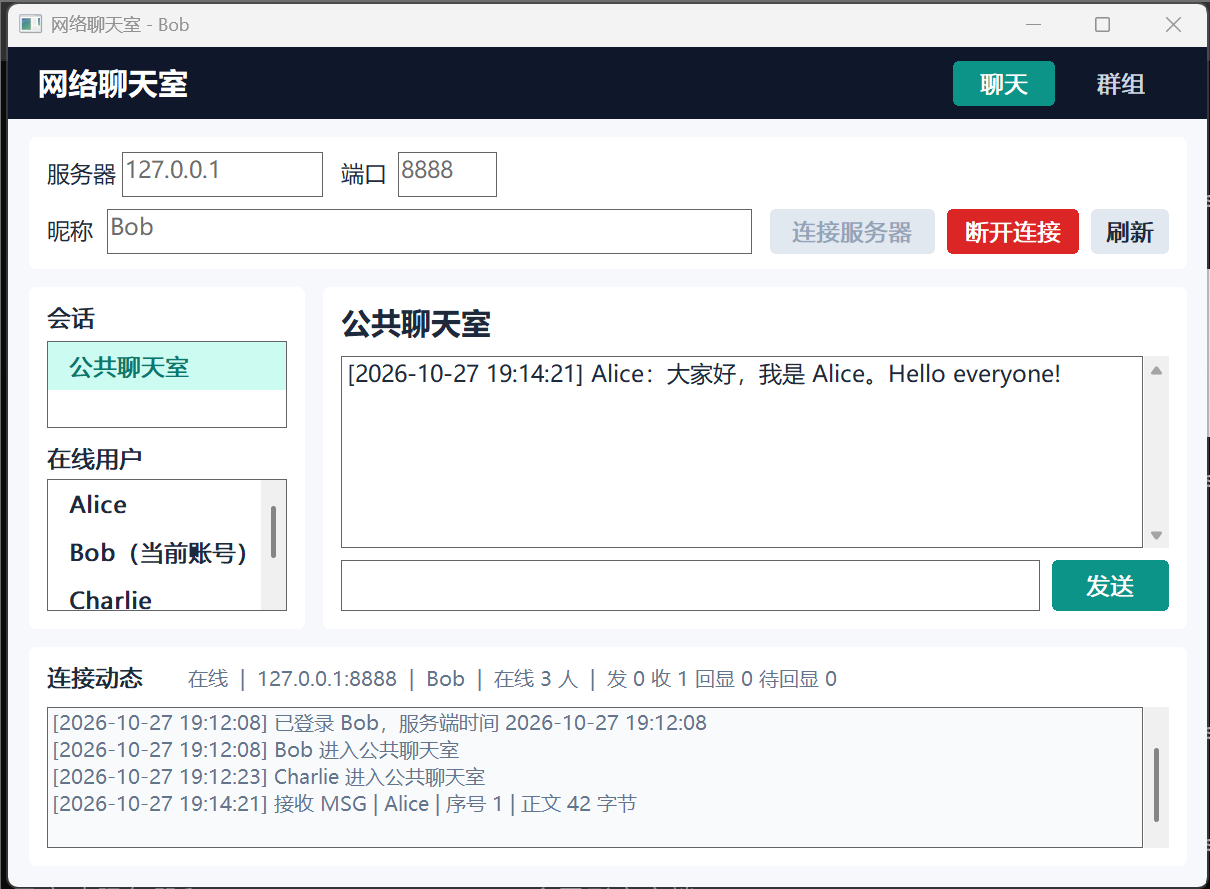
\includegraphics[width=\linewidth,height=10.0cm,keepaspectratio]{images/screen_06.png}
\captionof{figure}{Bob 收到 Alice 的公共发言}\label{fig:s06}
\par\smallskip{\raggedright\setlength{\parindent}{2em}\indent Bob 的公共会话中出现 Alice 的同一条发言，正文和时间同发送端一致。\par}
\end{minipage}\par\smallskip
\par\smallskip\noindent\begin{minipage}{\linewidth}\centering
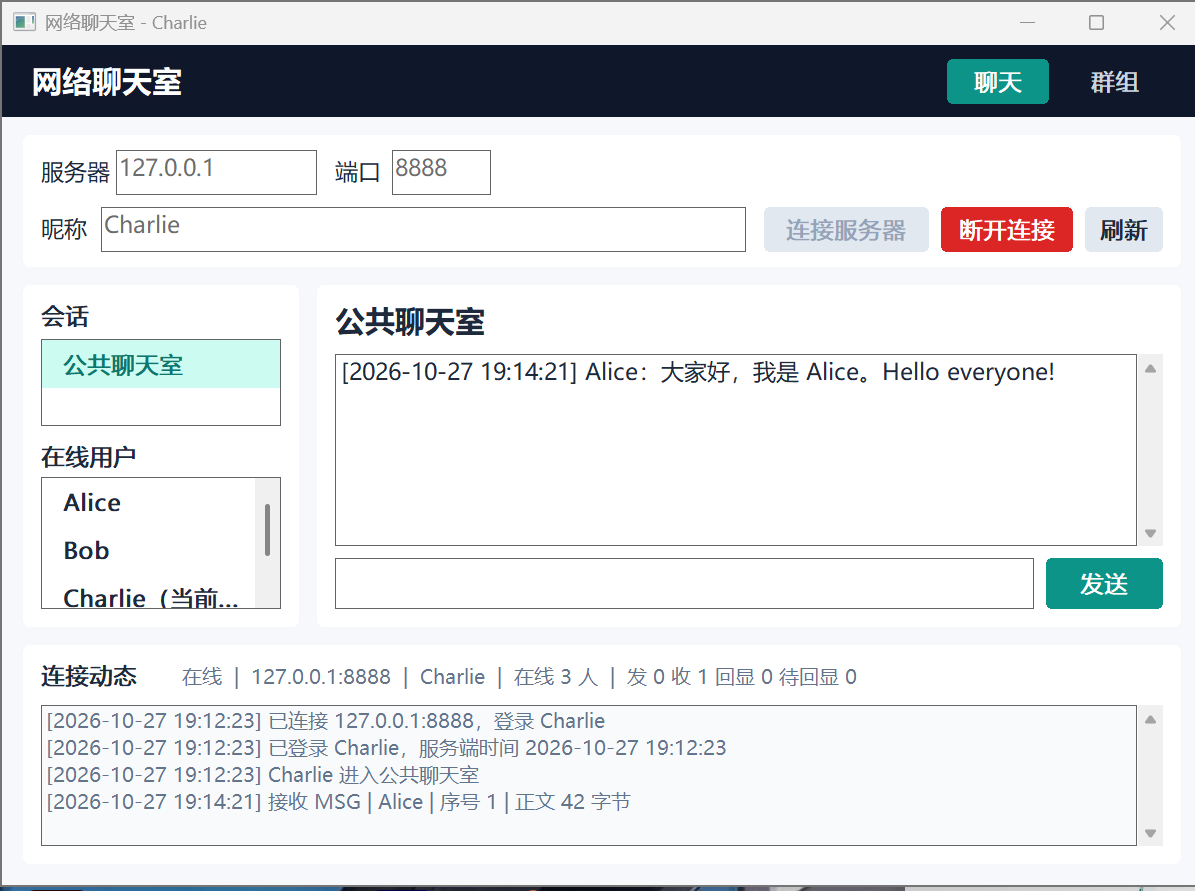
\includegraphics[width=\linewidth,height=10.0cm,keepaspectratio]{images/screen_07.png}
\captionof{figure}{Charlie 收到 Alice 的公共发言}\label{fig:s07}
\par\smallskip{\raggedright\setlength{\parindent}{2em}\indent Charlie 也显示这条消息，一次公共发言在三个窗口中均已送达。\par}
\end{minipage}\par\smallskip
Alice 的发言在三个窗口中显示相同正文和时间，随后由 Bob 继续回复，公共聊天也能够从第二条连接发起。

\par\smallskip\noindent\begin{minipage}{\linewidth}\centering
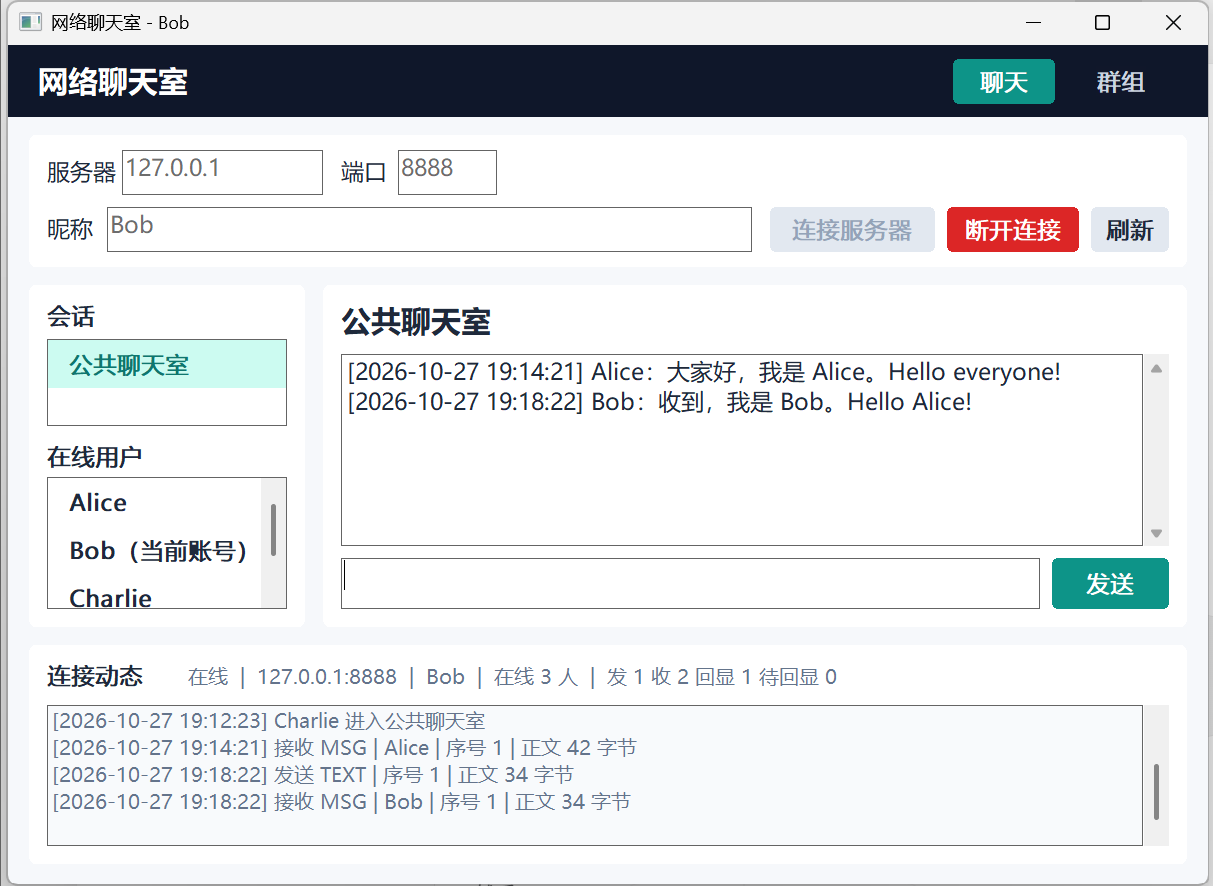
\includegraphics[width=\linewidth,height=10.0cm,keepaspectratio]{images/screen_08.png}
\captionof{figure}{Bob 的公共回复}\label{fig:s08}
\par\smallskip{\raggedright\setlength{\parindent}{2em}\indent Bob 输入中英文回复后，在本人公共会话中出现新的发言及服务器回显。\par}
\end{minipage}\par\smallskip
\par\smallskip\noindent\begin{minipage}{\linewidth}\centering
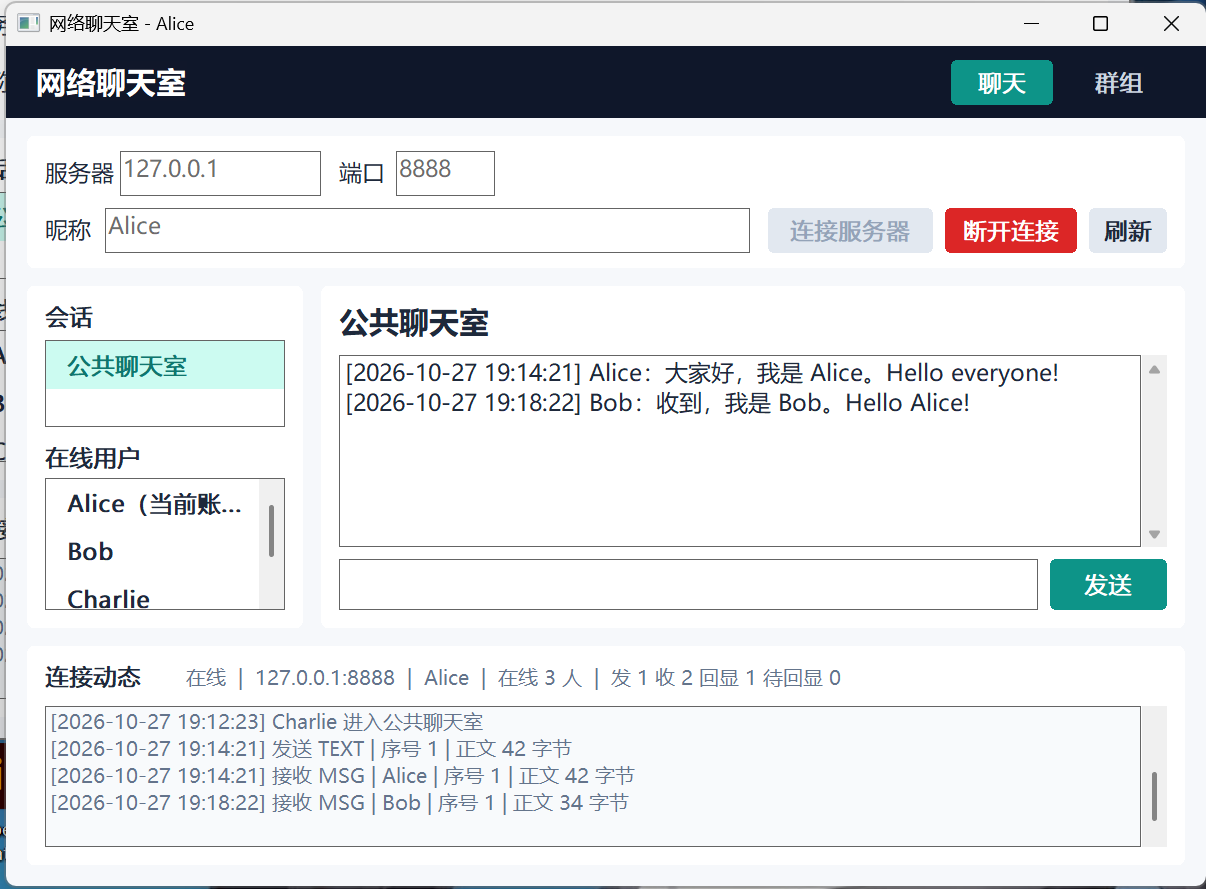
\includegraphics[width=\linewidth,height=10.0cm,keepaspectratio]{images/screen_09.png}
\captionof{figure}{Alice 收到 Bob 的回复}\label{fig:s09}
\par\smallskip{\raggedright\setlength{\parindent}{2em}\indent Alice 的聊天记录增加 Bob 的回复，动态区同时增加 MSG 接收记录。\par}
\end{minipage}\par\smallskip
\par\smallskip\noindent\begin{minipage}{\linewidth}\centering
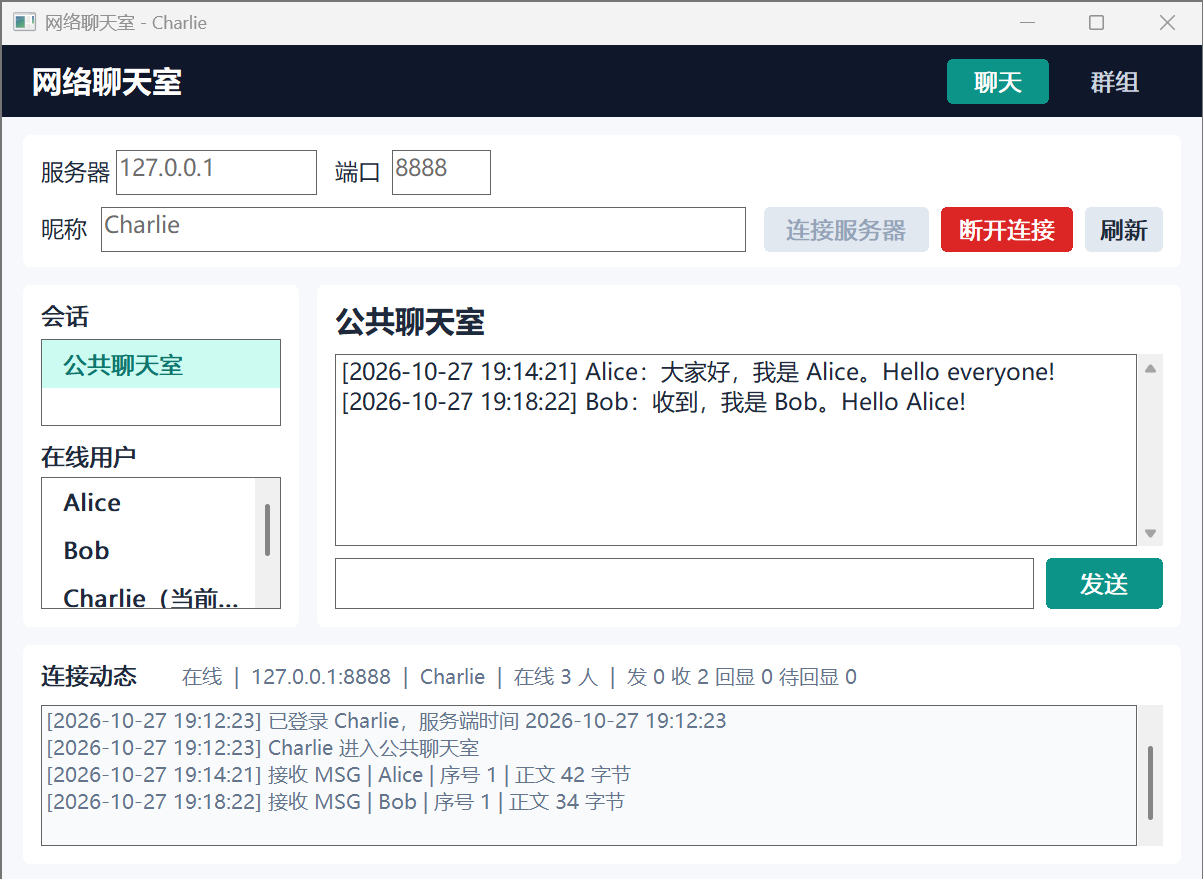
\includegraphics[width=\linewidth,height=10.0cm,keepaspectratio]{images/screen_10.png}
\captionof{figure}{Charlie 收到 Bob 的回复}\label{fig:s10}
\par\smallskip{\raggedright\setlength{\parindent}{2em}\indent Charlie 也收到 Bob 的回复，三条连接上的公共历史继续保持对应。\par}
\end{minipage}\par\smallskip
最后使用 Charlie 发言，在 Bob 和 Alice 中也出现相同消息，至此三位用户都完成了一次发送，并接收到另外两人的发言。

\par\smallskip\noindent\begin{minipage}{\linewidth}\centering
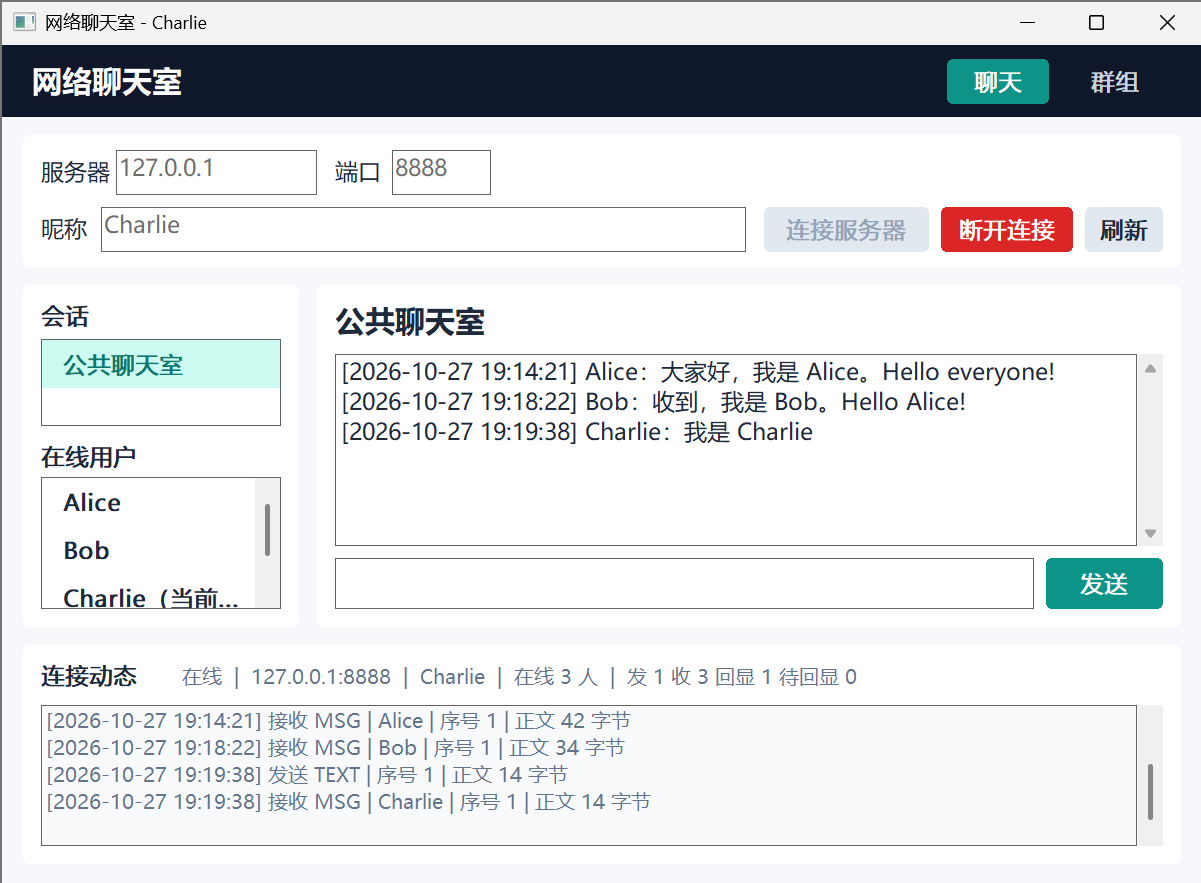
\includegraphics[width=\linewidth,height=10.0cm,keepaspectratio]{images/screen_11.png}
\captionof{figure}{Charlie 的公共发言}\label{fig:s11}
\par\smallskip{\raggedright\setlength{\parindent}{2em}\indent Charlie 发言后，本人窗口出现带服务器时间的消息，下方记录发送及回显。\par}
\end{minipage}\par\smallskip
\par\smallskip\noindent\begin{minipage}{\linewidth}\centering
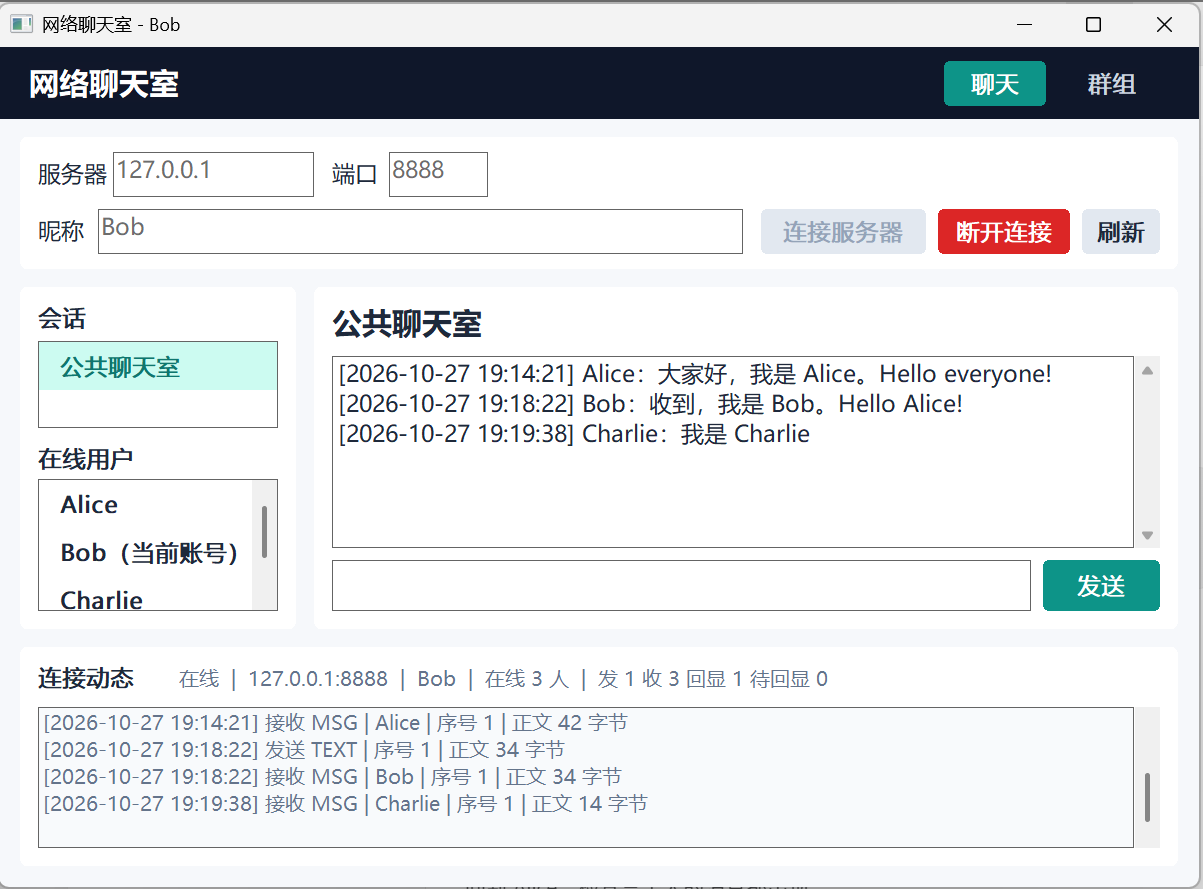
\includegraphics[width=\linewidth,height=10.0cm,keepaspectratio]{images/screen_12.png}
\captionof{figure}{Bob 收到 Charlie 的发言}\label{fig:s12}
\par\smallskip{\raggedright\setlength{\parindent}{2em}\indent Bob 的公共会话新增 Charlie 的发言，当前已经包含三位用户的消息。\par}
\end{minipage}\par\smallskip
\par\smallskip\noindent\begin{minipage}{\linewidth}\centering
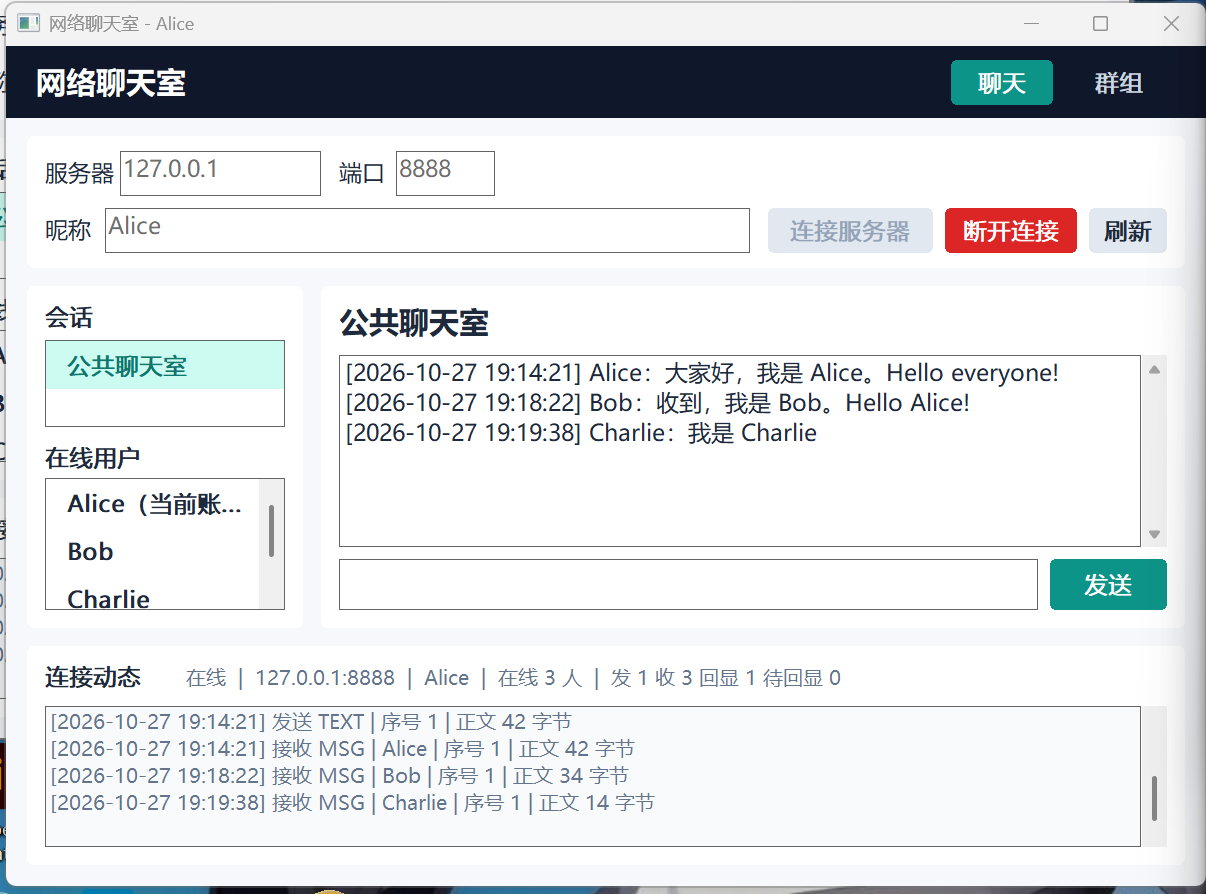
\includegraphics[width=\linewidth,height=10.0cm,keepaspectratio]{images/screen_13.png}
\captionof{figure}{Alice 中的三人公共历史}\label{fig:s13}
\par\smallskip{\raggedright\setlength{\parindent}{2em}\indent Alice 中同样呈现三人的发言，中文、英文及时间均能正常显示。\par}
\end{minipage}\par\smallskip
\subsection{私聊}
在 Alice 的在线名单中点击 Bob 后，右侧切换为私聊，发送的中英文正文出现在 Alice、Bob 的会话中；同时保留 Charlie 的公共页面，记录另一用户的消息状态。

\par\smallskip\noindent\begin{minipage}{\linewidth}\centering
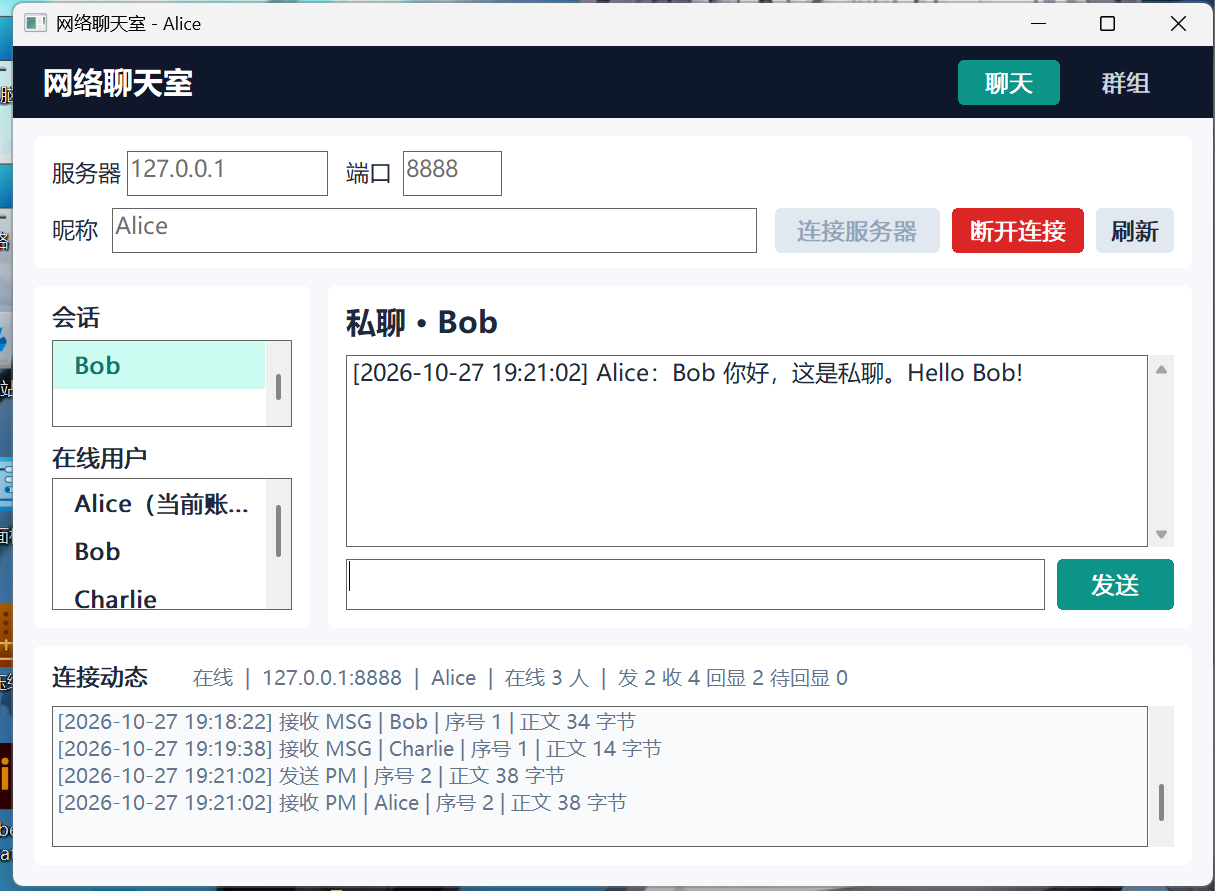
\includegraphics[width=\linewidth,height=10.0cm,keepaspectratio]{images/screen_14.png}
\captionof{figure}{Alice 发给 Bob 的私聊}\label{fig:s14}
\par\smallskip{\raggedright\setlength{\parindent}{2em}\indent Alice 点击 Bob 后进入独立私聊，发送的消息显示在 Bob 会话中，标题也随所选联系人变化。\par}
\end{minipage}\par\smallskip
\par\smallskip\noindent\begin{minipage}{\linewidth}\centering
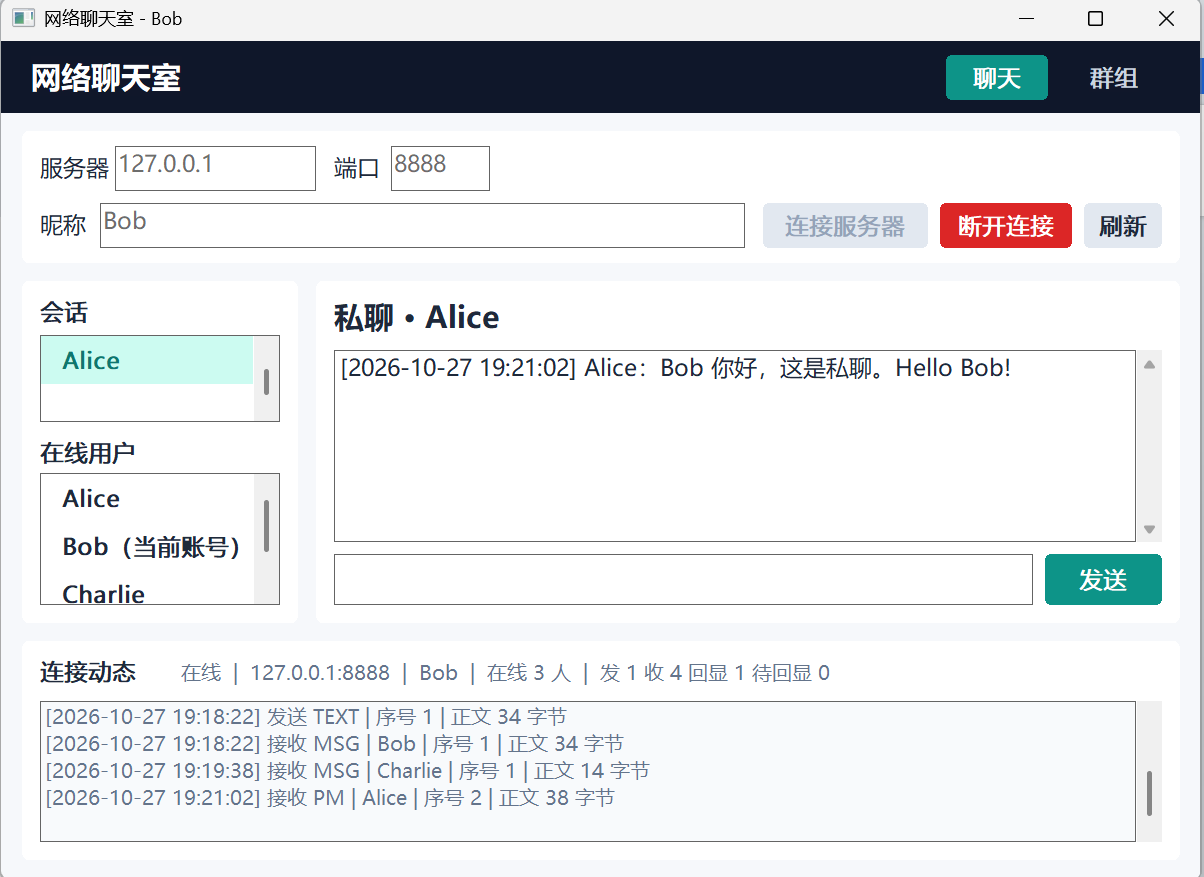
\includegraphics[width=\linewidth,height=10.0cm,keepaspectratio]{images/screen_15.png}
\captionof{figure}{Bob 收到 Alice 的私聊}\label{fig:s15}
\par\smallskip{\raggedright\setlength{\parindent}{2em}\indent 在 Bob 中选择 Alice 后，可以看到刚收到的中英文私聊，发送者和正文同 Alice 的记录对应。\par}
\end{minipage}\par\smallskip
\par\smallskip\noindent\begin{minipage}{\linewidth}\centering
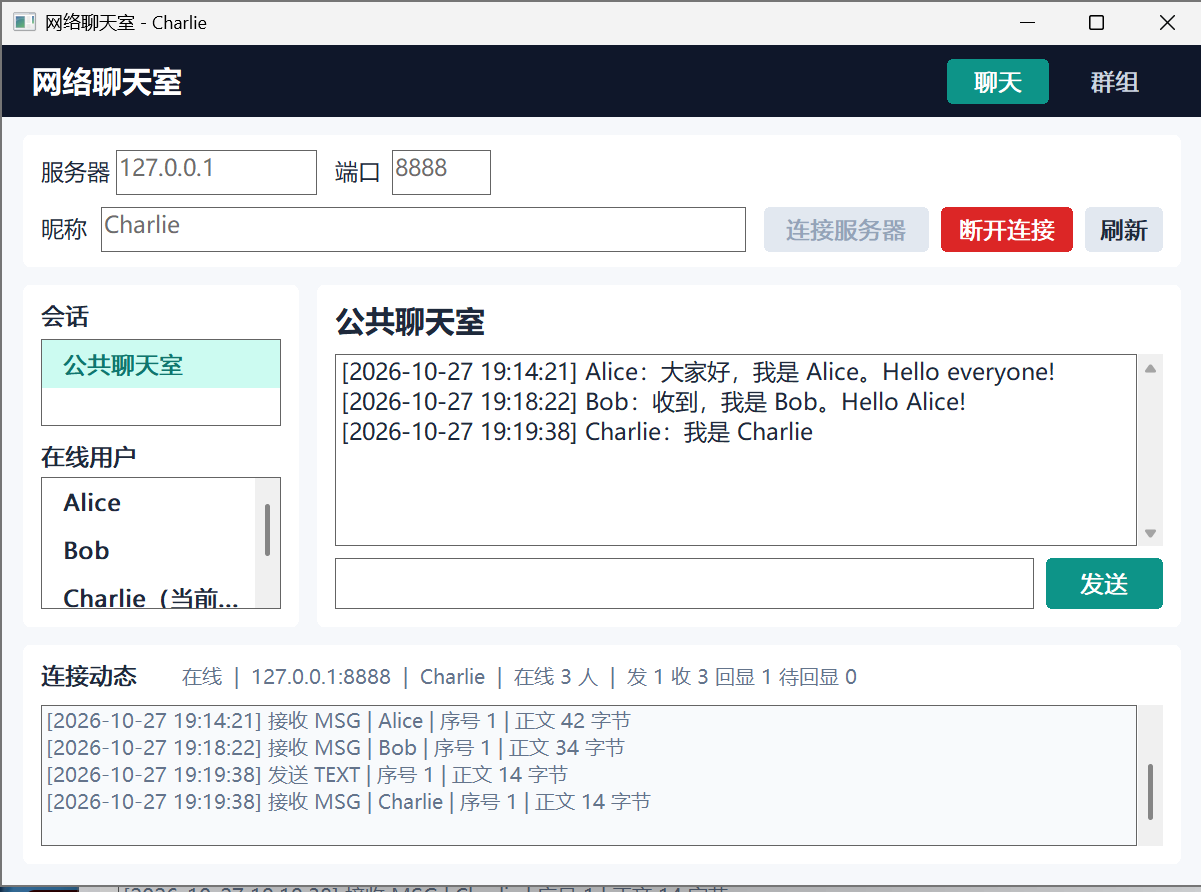
\includegraphics[width=\linewidth,height=10.0cm,keepaspectratio]{images/screen_16.png}
\captionof{figure}{Charlie 在私聊期间的公共页面}\label{fig:s16}
\par\smallskip{\raggedright\setlength{\parindent}{2em}\indent 与此同时，Charlie 的公共页面仍保留三条公共消息，接收数为 3。\par}
\end{minipage}\par\smallskip
Bob 回复后，双方私聊中都能看到两人的对话，而 Charlie 仍保留原来的公共记录，接收数保持为 3，呈现了按目标会话转发的范围。

\par\smallskip\noindent\begin{minipage}{\linewidth}\centering
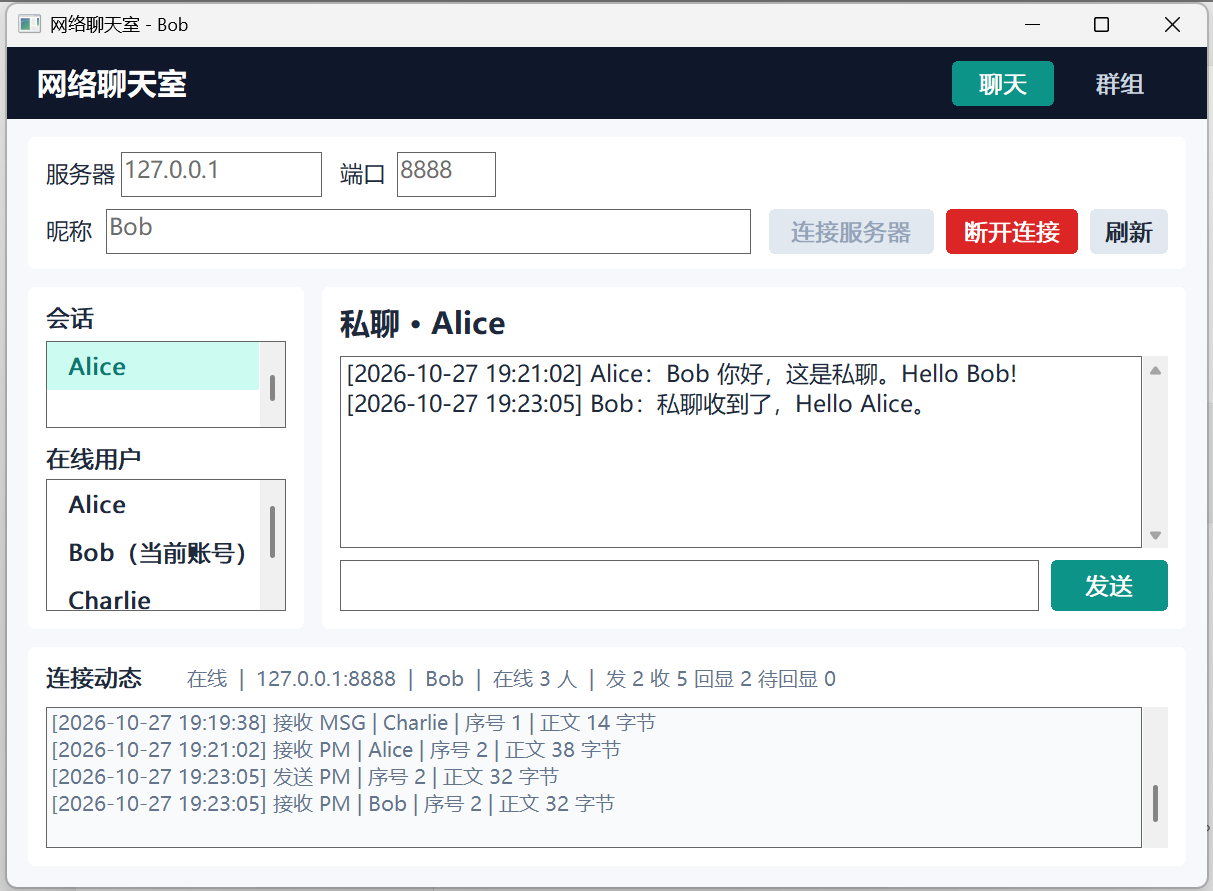
\includegraphics[width=\linewidth,height=10.0cm,keepaspectratio]{images/screen_17.png}
\captionof{figure}{Bob 的私聊回复}\label{fig:s17}
\par\smallskip{\raggedright\setlength{\parindent}{2em}\indent Bob 回复后，Alice 私聊历史中出现双方的发言，记录按同一联系人连续保存。\par}
\end{minipage}\par\smallskip
\par\smallskip\noindent\begin{minipage}{\linewidth}\centering
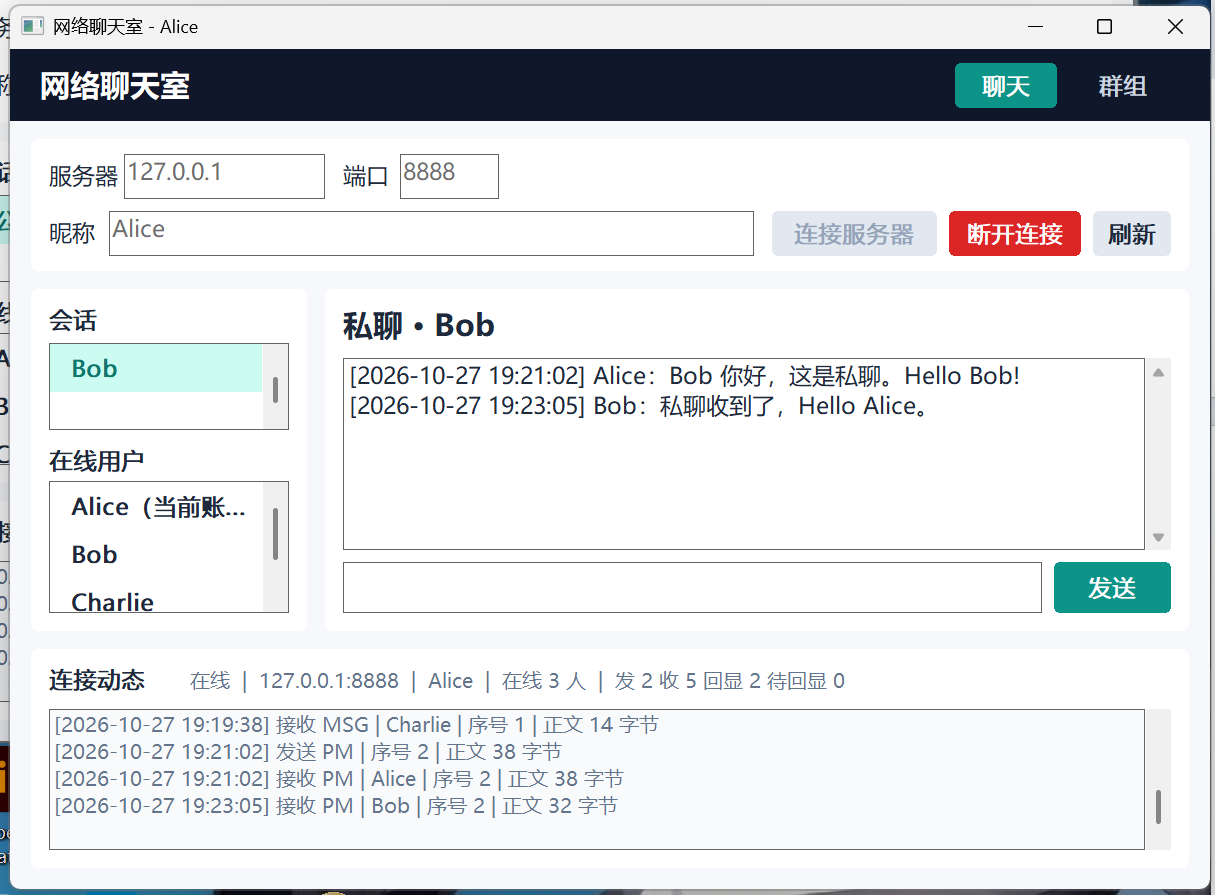
\includegraphics[width=\linewidth,height=10.0cm,keepaspectratio]{images/screen_18.png}
\captionof{figure}{Alice 收到私聊回复}\label{fig:s18}
\par\smallskip{\raggedright\setlength{\parindent}{2em}\indent Alice 收到 Bob 的回复，双方窗口中都能看到这段对话。\par}
\end{minipage}\par\smallskip
\par\smallskip\noindent\begin{minipage}{\linewidth}\centering
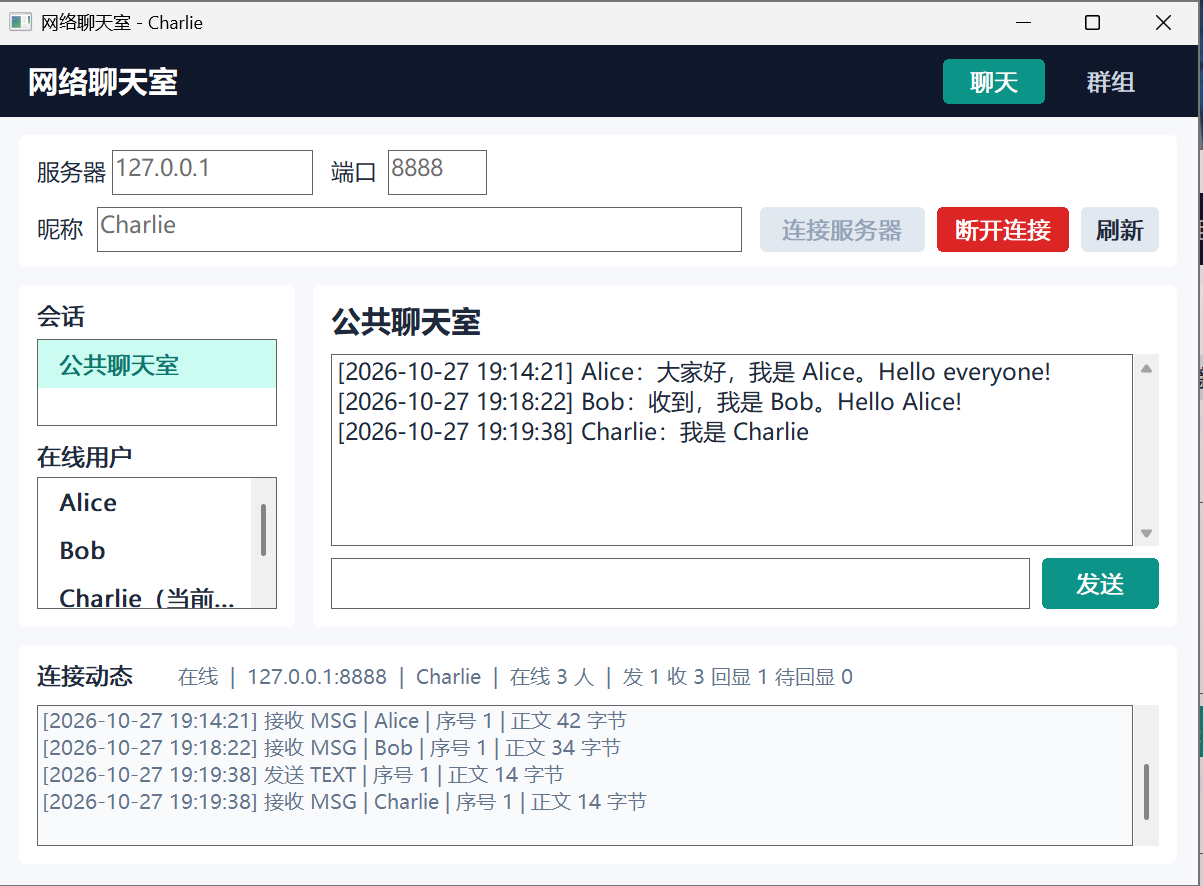
\includegraphics[width=\linewidth,height=10.0cm,keepaspectratio]{images/screen_19.png}
\captionof{figure}{Charlie 的公共历史保持原样}\label{fig:s19}
\par\smallskip{\raggedright\setlength{\parindent}{2em}\indent Charlie 仍呈现原来的三条公共消息，接收数保持为 3，体现了这段私聊的定向转发范围。\par}
\end{minipage}\par\smallskip
\subsection{会话切换}
在 Alice 中由 Bob 私聊切回公共聊天室，再选回 Bob，右侧分别呈现三人的公共发言和双方私聊，之前的历史都随所选会话保留。

\par\smallskip\noindent\begin{minipage}{\linewidth}\centering
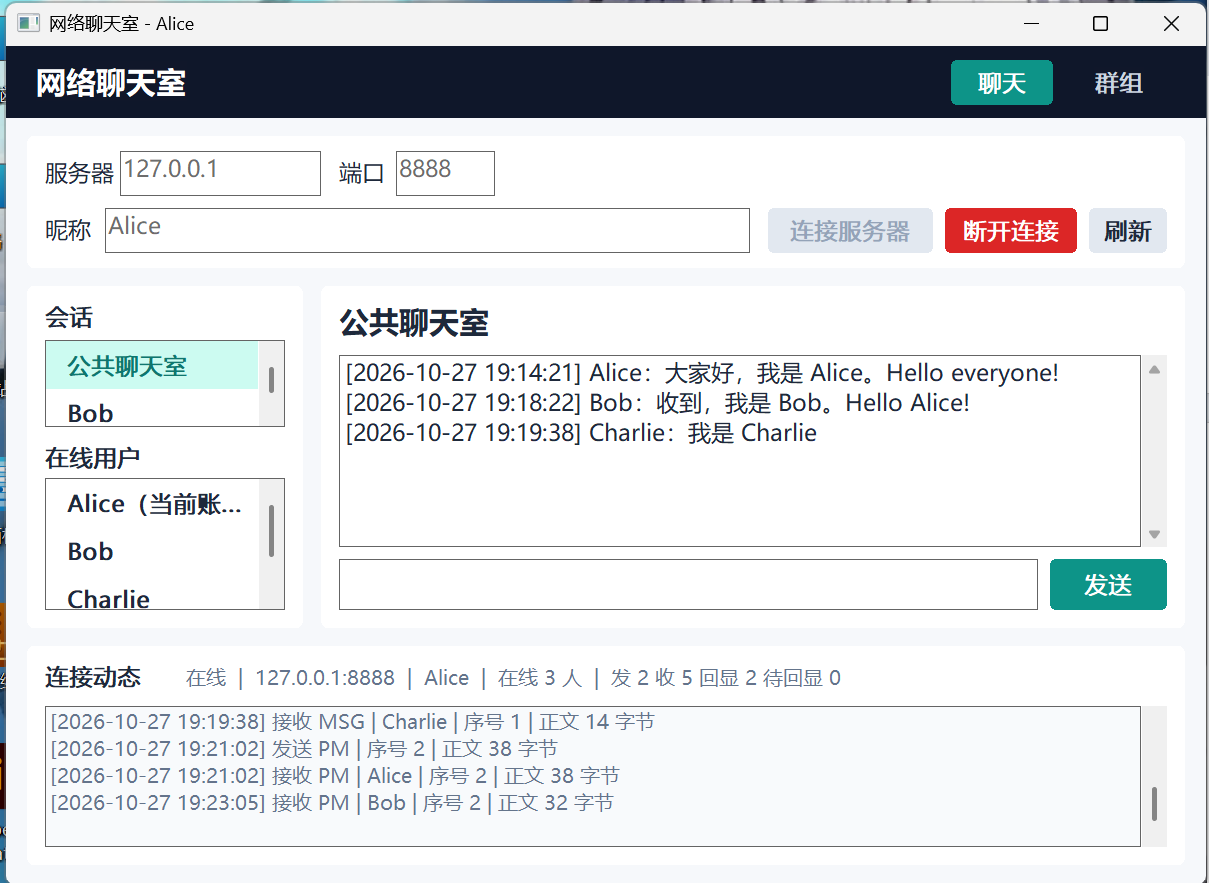
\includegraphics[width=\linewidth,height=10.0cm,keepaspectratio]{images/screen_20.png}
\captionof{figure}{Alice 切回公共会话}\label{fig:s20}
\par\smallskip{\raggedright\setlength{\parindent}{2em}\indent Alice 切回公共聊天室后，三人的公共历史重新显示在右侧。\par}
\end{minipage}\par\smallskip
\par\smallskip\noindent\begin{minipage}{\linewidth}\centering
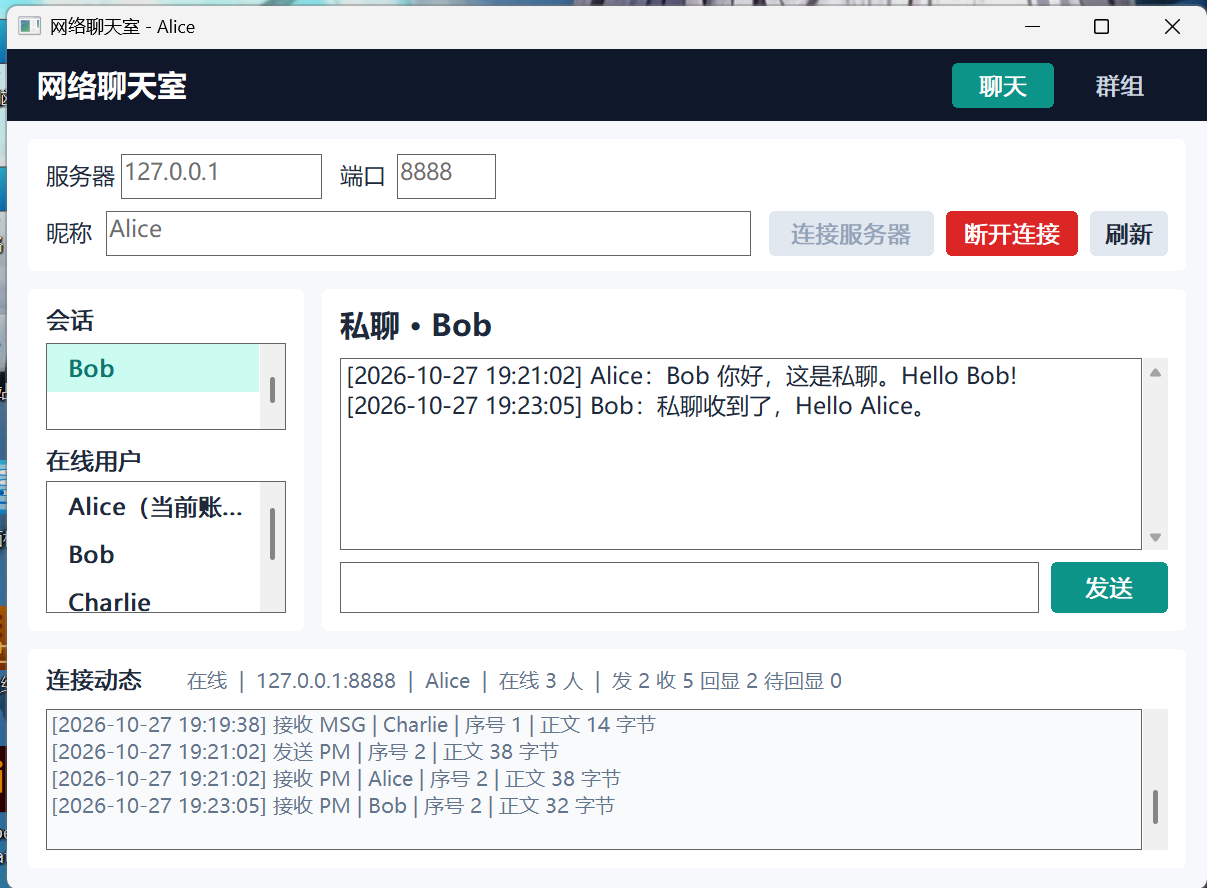
\includegraphics[width=\linewidth,height=10.0cm,keepaspectratio]{images/screen_21.png}
\captionof{figure}{Alice 切回 Bob 私聊}\label{fig:s21}
\par\smallskip{\raggedright\setlength{\parindent}{2em}\indent 再次选择 Bob 后，右侧恢复双方私聊，切换会话期间保留了原记录。\par}
\end{minipage}\par\smallskip
\subsection{建立群聊}
在 Alice 的群页面输入 Chat1 并建立群聊后，左侧出现群名，下方显示创建成功；继续选择 Bob 并添加，动态区随即出现成员变更提示。

\par\smallskip\noindent\begin{minipage}{\linewidth}\centering
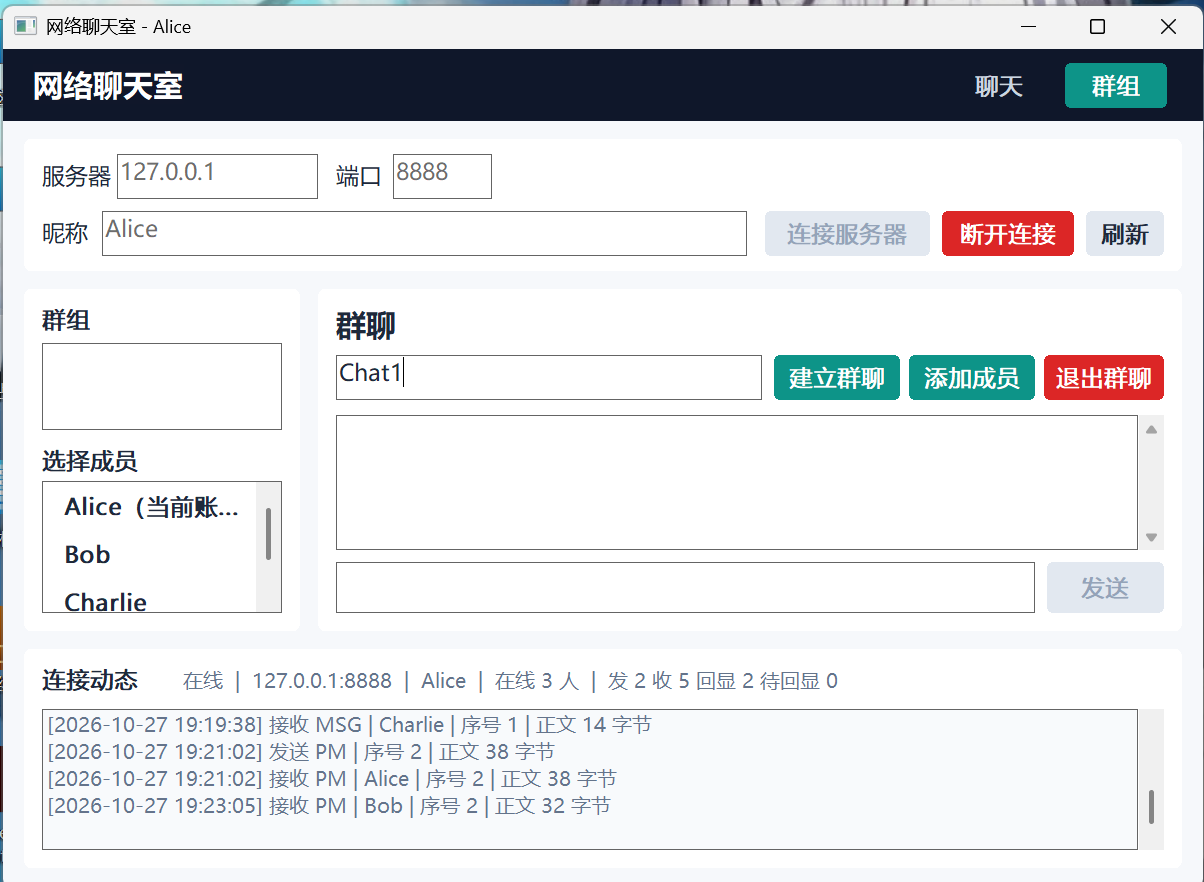
\includegraphics[width=\linewidth,height=10.0cm,keepaspectratio]{images/screen_22.png}
\captionof{figure}{Chat1 创建前的群页面}\label{fig:s22}
\par\smallskip{\raggedright\setlength{\parindent}{2em}\indent 在群页面中输入 Chat1，此时已填写群名，接下来执行建立群聊。\par}
\end{minipage}\par\smallskip
\par\smallskip\noindent\begin{minipage}{\linewidth}\centering
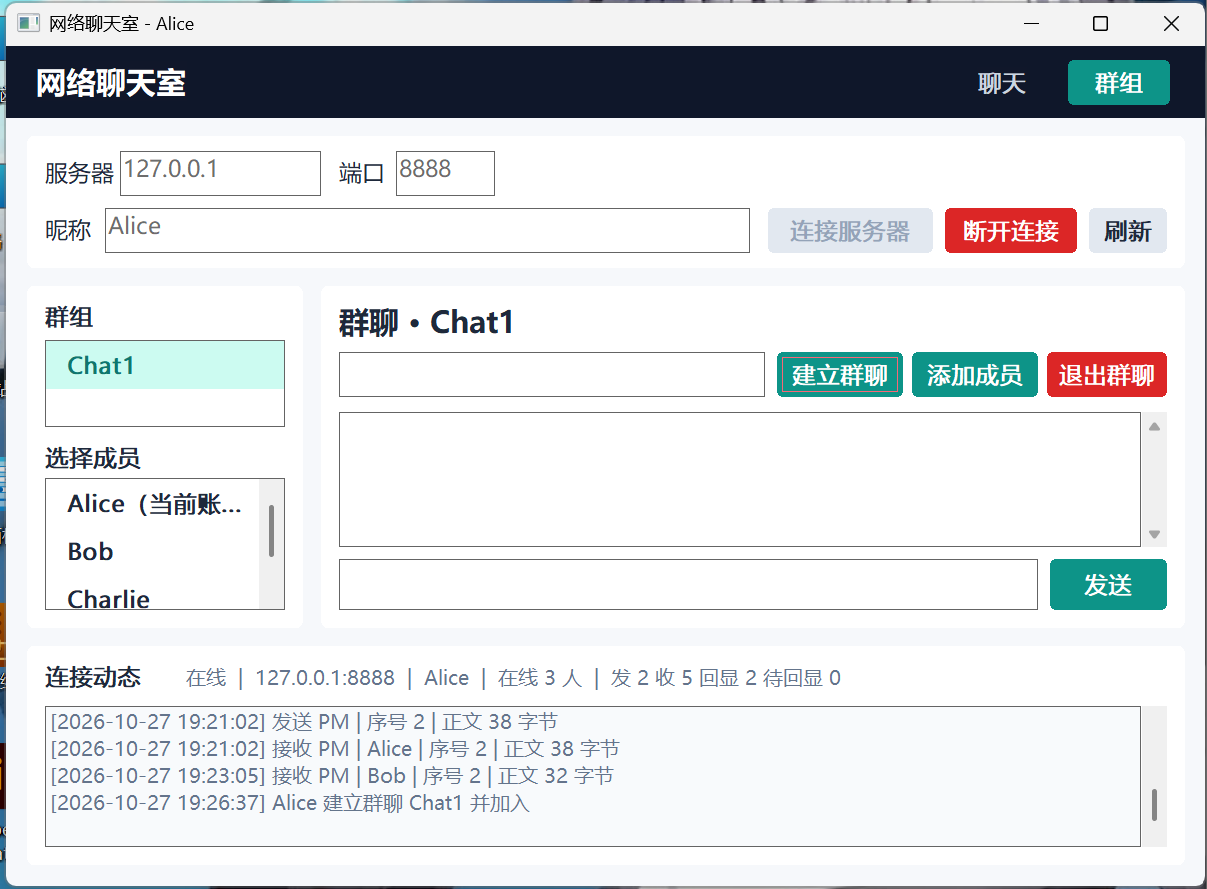
\includegraphics[width=\linewidth,height=10.0cm,keepaspectratio]{images/screen_23.png}
\captionof{figure}{Chat1 创建成功}\label{fig:s23}
\par\smallskip{\raggedright\setlength{\parindent}{2em}\indent 点击建立群聊后，左侧出现 Chat1，底部显示创建成功及创建者入群提示。\par}
\end{minipage}\par\smallskip
\par\smallskip\noindent\begin{minipage}{\linewidth}\centering
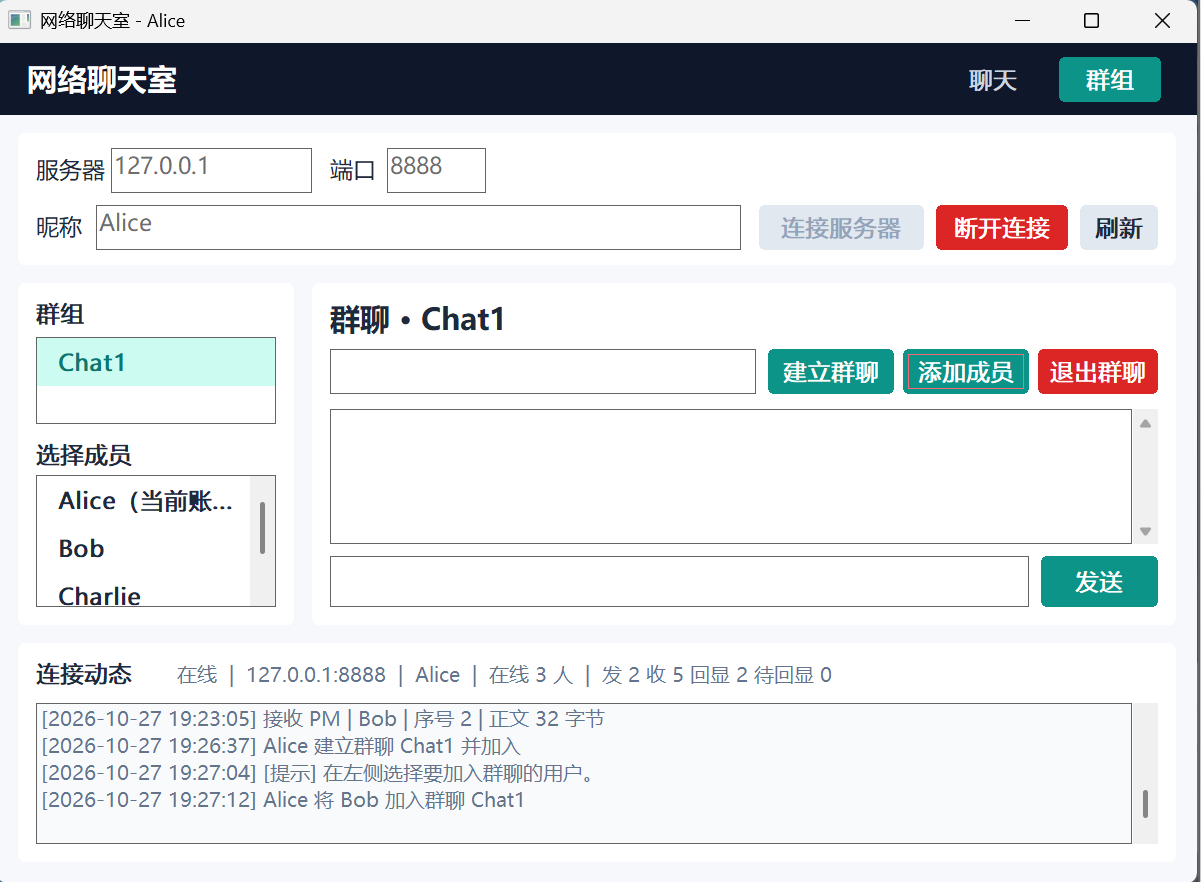
\includegraphics[width=\linewidth,height=10.0cm,keepaspectratio]{images/screen_24.png}
\captionof{figure}{Bob 加入 Chat1}\label{fig:s24}
\par\smallskip{\raggedright\setlength{\parindent}{2em}\indent 添加 Bob 后，底部出现对应成员通知，Chat1 已由 Alice、Bob 两位成员组成。\par}
\end{minipage}\par\smallskip
此时 Alice、Bob 已是群成员，接下来在两人之间发送群消息，同时记录 Charlie 加入前的页面，观察成员增加前后的接收变化。

\subsection{群消息}
Alice 在 Chat1 发送中英文正文后，底部出现 GTEXT、GMSG，Bob 打开 Chat1 也能看到这条群消息；Charlie 此时尚未加入，群页面保持原状态。

\par\smallskip\noindent\begin{minipage}{\linewidth}\centering
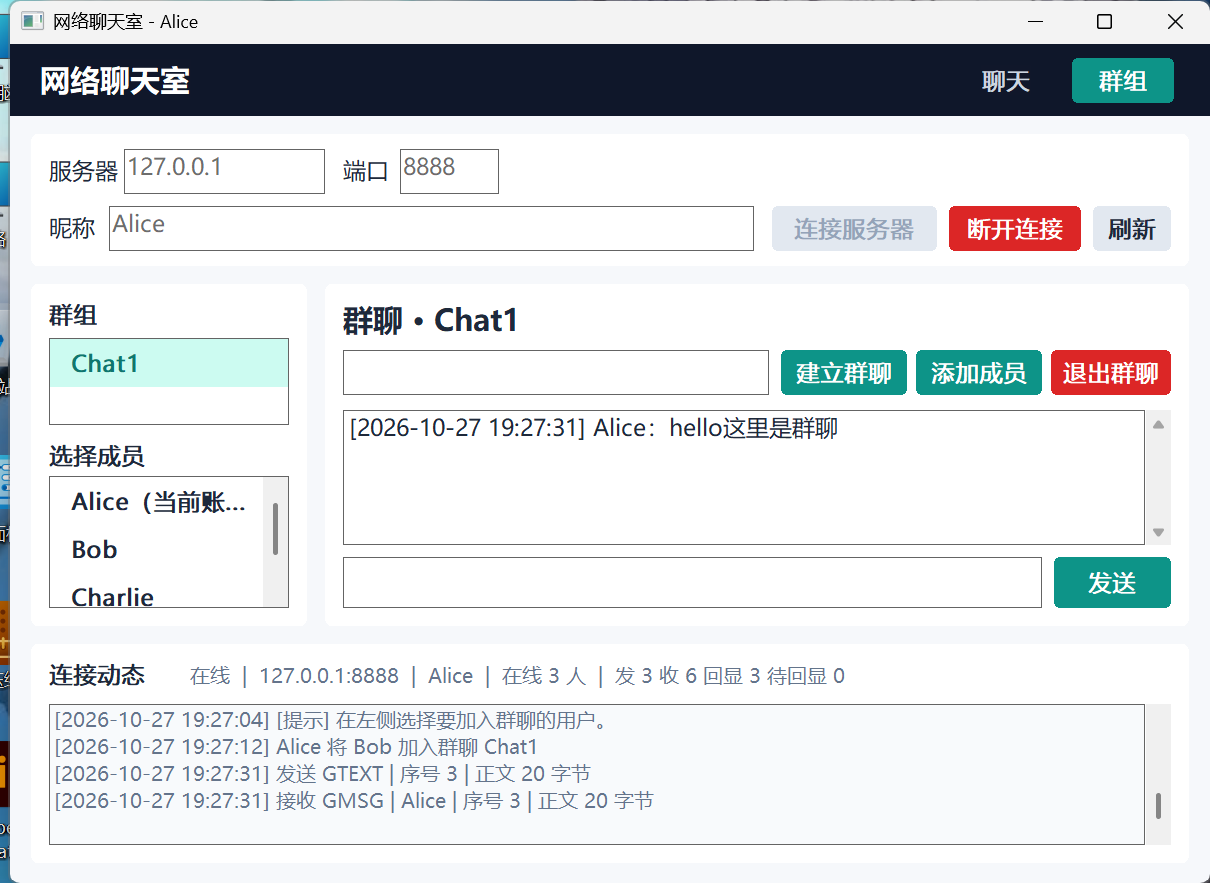
\includegraphics[width=\linewidth,height=10.0cm,keepaspectratio]{images/screen_25.png}
\captionof{figure}{Alice 的中英文群发言}\label{fig:s25}
\par\smallskip{\raggedright\setlength{\parindent}{2em}\indent Alice 在 Chat1 发送中英文消息后，群会话出现本人正文，动态区记录 GTEXT 和 GMSG。\par}
\end{minipage}\par\smallskip
\par\smallskip\noindent\begin{minipage}{\linewidth}\centering
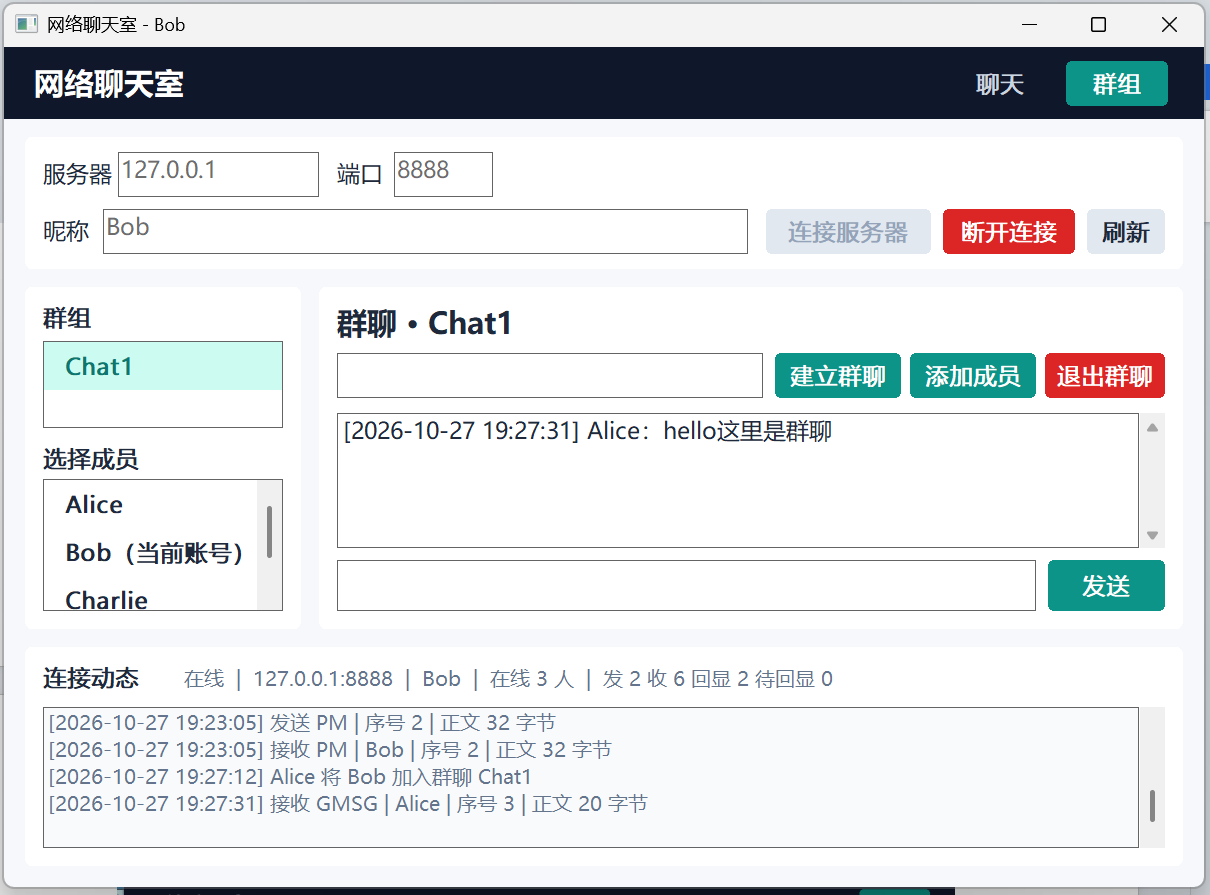
\includegraphics[width=\linewidth,height=10.0cm,keepaspectratio]{images/screen_26.png}
\captionof{figure}{Bob 收到群消息}\label{fig:s26}
\par\smallskip{\raggedright\setlength{\parindent}{2em}\indent Bob 打开 Chat1 后收到 Alice 的群消息，加入群的另一位成员已经收到正文。\par}
\end{minipage}\par\smallskip
\par\smallskip\noindent\begin{minipage}{\linewidth}\centering
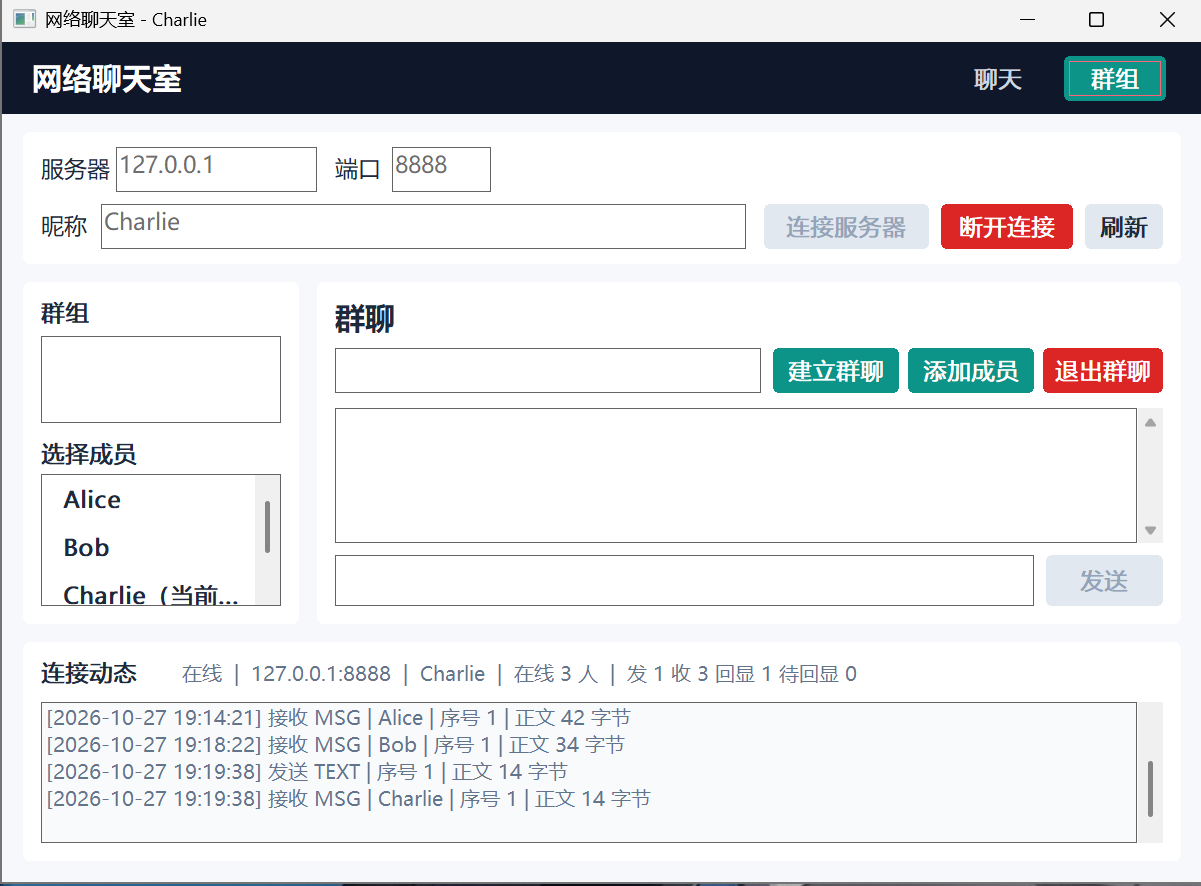
\includegraphics[width=\linewidth,height=10.0cm,keepaspectratio]{images/screen_27.png}
\captionof{figure}{Charlie 加入群前的页面}\label{fig:s27}
\par\smallskip{\raggedright\setlength{\parindent}{2em}\indent 此时 Charlie 的群列表仍为空，页面保留加入 Chat1 之前的状态。\par}
\end{minipage}\par\smallskip
\subsection{添加第三位成员}
将 Charlie 加入 Chat1 后，先在 Alice 中出现入群提示，再由 Bob 发送欢迎消息。Alice 和 Charlie 都收到了这一新发言，群聊由两位成员扩展为三位。

\par\smallskip\noindent\begin{minipage}{\linewidth}\centering
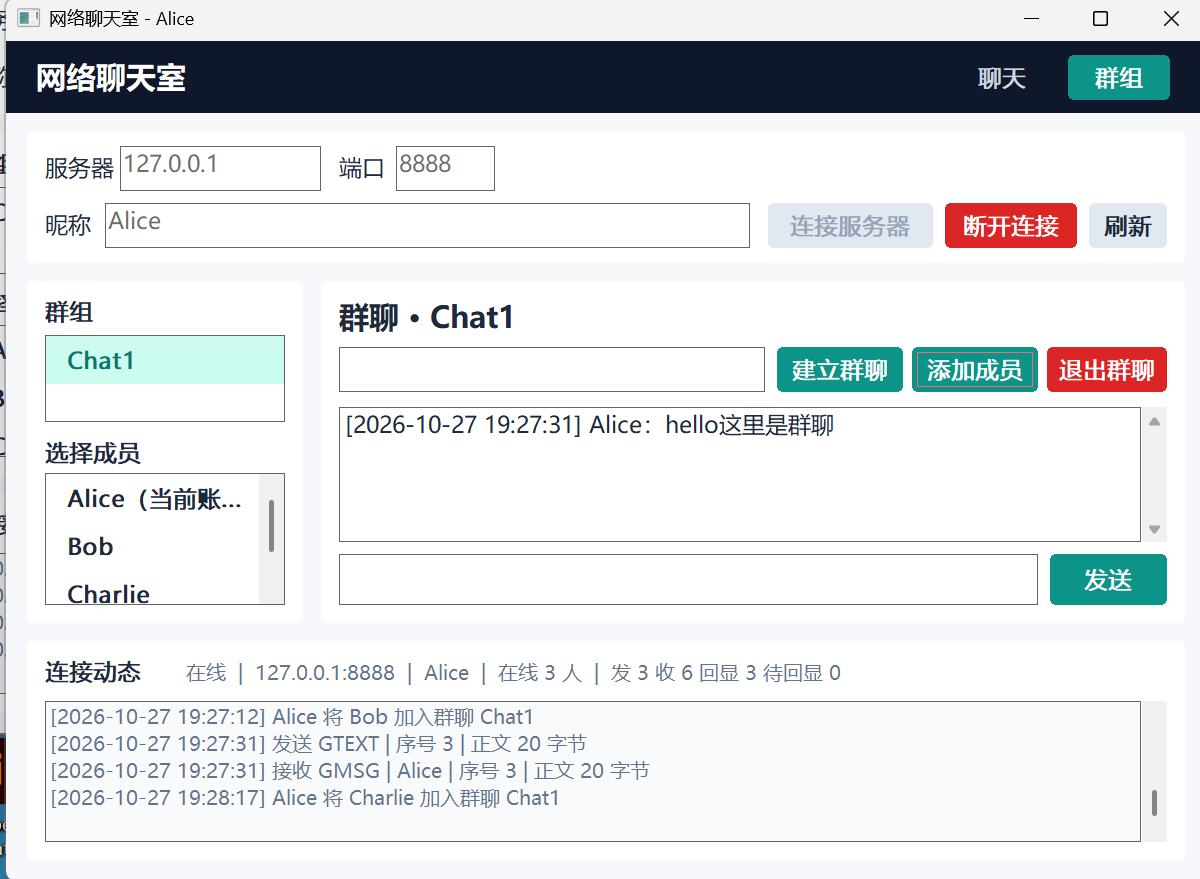
\includegraphics[width=\linewidth,height=10.0cm,keepaspectratio]{images/screen_28.png}
\captionof{figure}{Charlie 加入 Chat1}\label{fig:s28}
\par\smallskip{\raggedright\setlength{\parindent}{2em}\indent Alice 添加 Charlie 后，底部出现 Charlie 加入 Chat1 的通知。\par}
\end{minipage}\par\smallskip
\par\smallskip\noindent\begin{minipage}{\linewidth}\centering
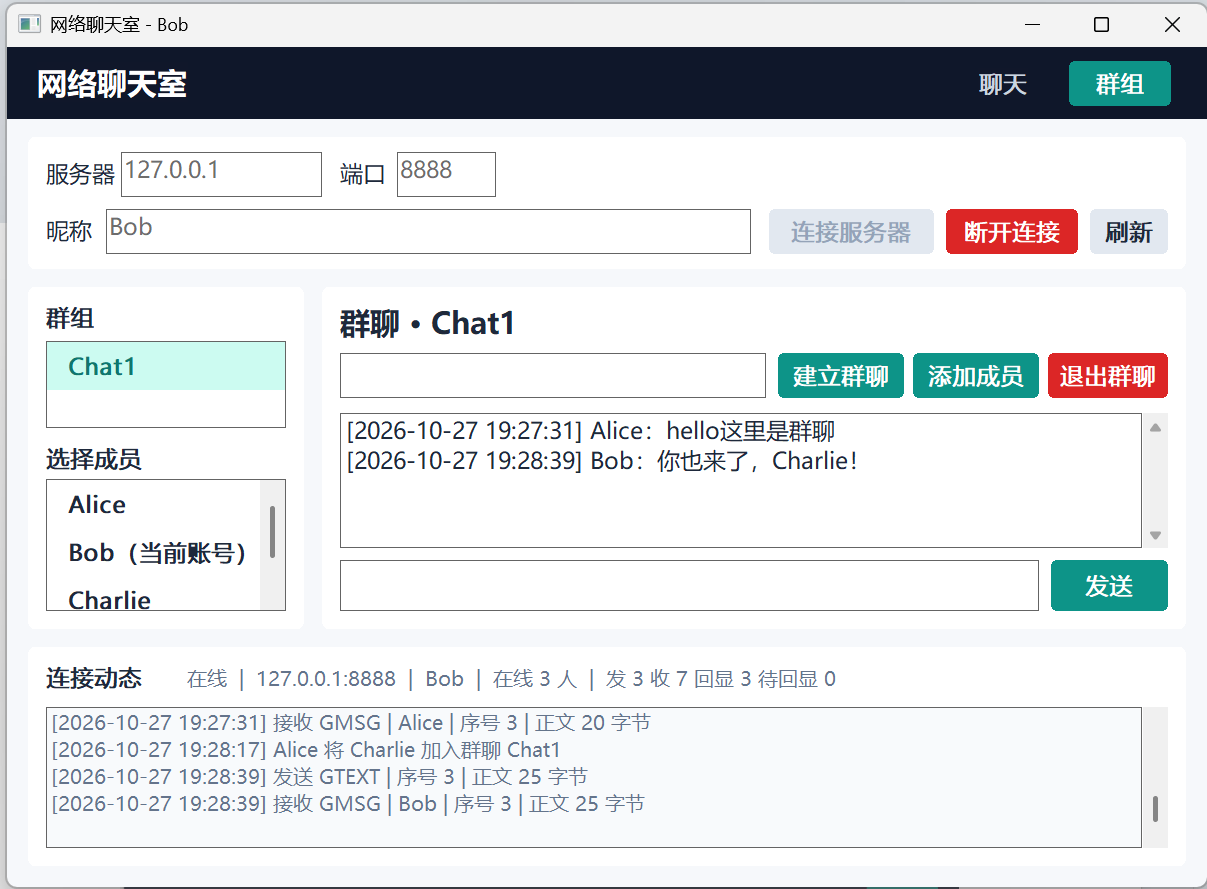
\includegraphics[width=\linewidth,height=10.0cm,keepaspectratio]{images/screen_29.png}
\captionof{figure}{Bob 在群中的欢迎消息}\label{fig:s29}
\par\smallskip{\raggedright\setlength{\parindent}{2em}\indent Bob 在群里发送欢迎消息，群历史随即增加本人发言及回显。\par}
\end{minipage}\par\smallskip
\par\smallskip\noindent\begin{minipage}{\linewidth}\centering
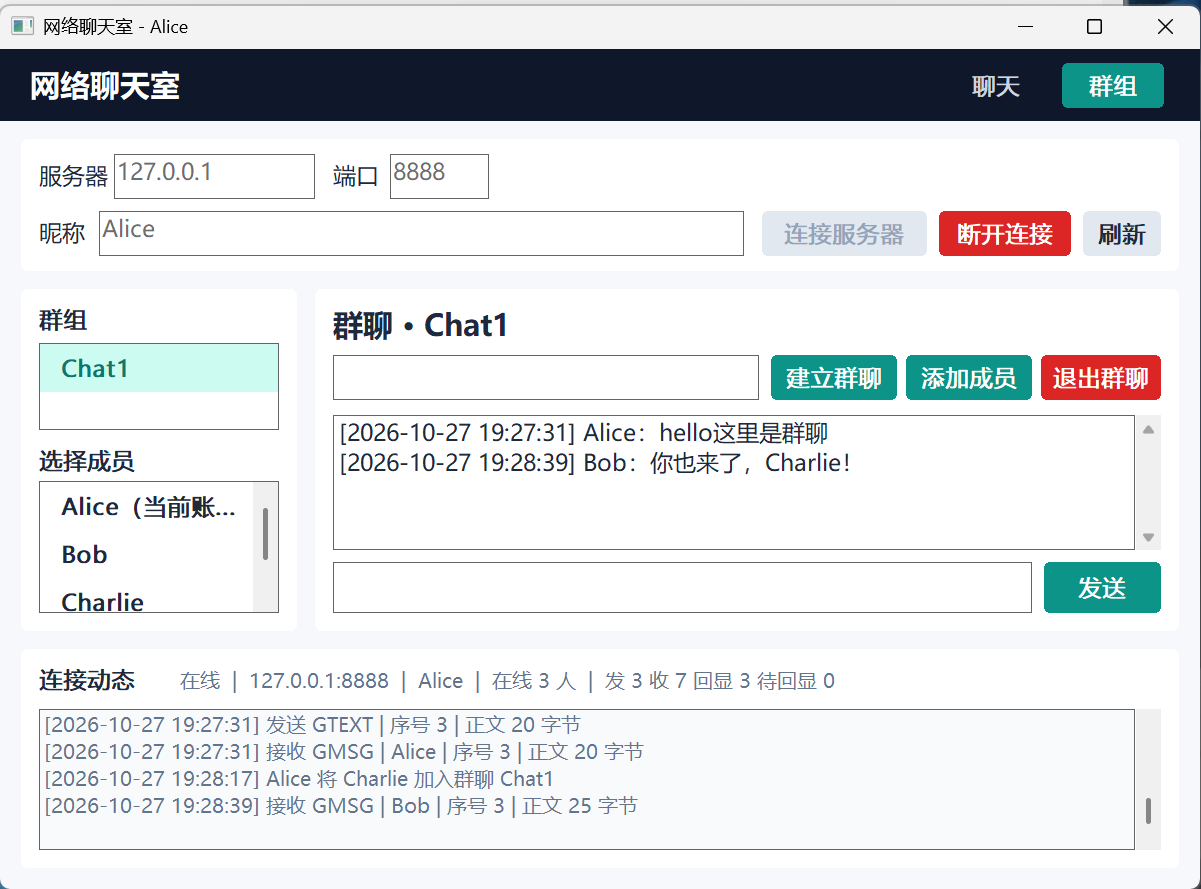
\includegraphics[width=\linewidth,height=10.0cm,keepaspectratio]{images/screen_30.png}
\captionof{figure}{Alice 收到 Bob 的群回复}\label{fig:s30}
\par\smallskip{\raggedright\setlength{\parindent}{2em}\indent Alice 收到 Bob 的欢迎消息，原有成员继续接收新的群发言。\par}
\end{minipage}\par\smallskip
\par\smallskip\noindent\begin{minipage}{\linewidth}\centering
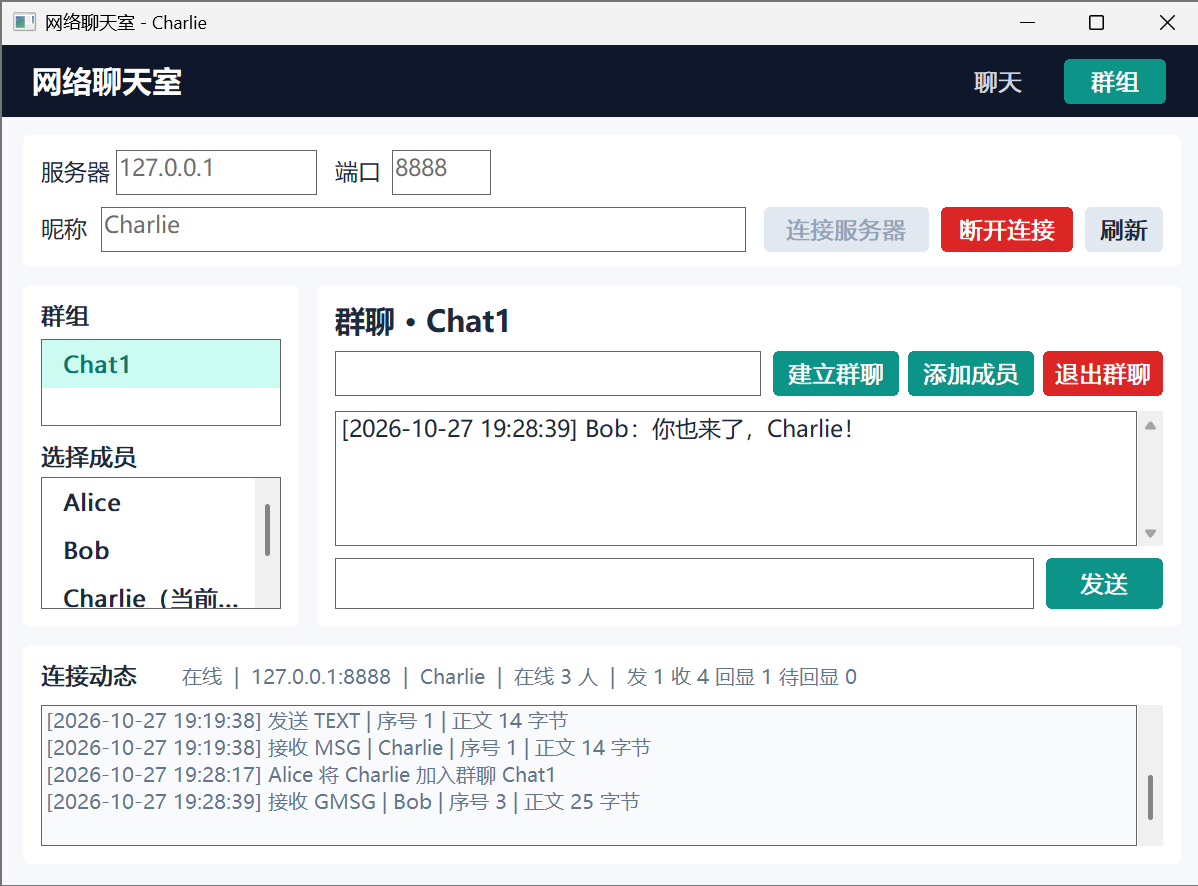
\includegraphics[width=\linewidth,height=10.0cm,keepaspectratio]{images/screen_31.png}
\captionof{figure}{Charlie 收到加入后的新消息}\label{fig:s31}
\par\smallskip{\raggedright\setlength{\parindent}{2em}\indent Charlie 的群历史从加入后的新消息开始，页面中可以看到 Bob 刚发送的欢迎内容。\par}
\end{minipage}\par\smallskip
在 Alice、Bob 中仍保留入群前的群消息，而 Charlie 的历史从加入后的新消息开始，体现了按当前成员即时转发的处理。

\subsection{退出群聊}
Charlie 点击退出群聊后，下方显示退出成功，Alice 收到相应通知并继续发送群消息，随后在 Bob 和 Charlie 中呈现不同接收状态。

\par\smallskip\noindent\begin{minipage}{\linewidth}\centering
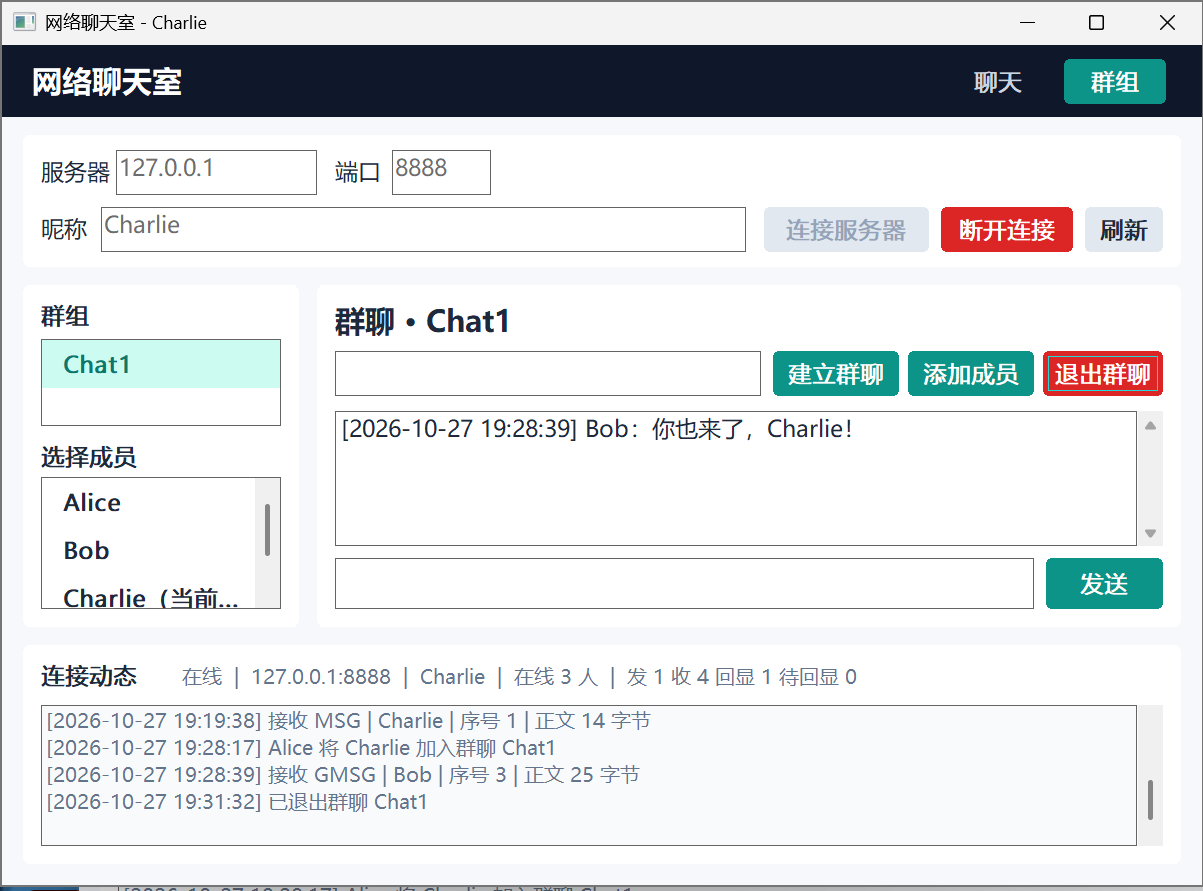
\includegraphics[width=\linewidth,height=10.0cm,keepaspectratio]{images/screen_32.png}
\captionof{figure}{Charlie 退出群聊}\label{fig:s32}
\par\smallskip{\raggedright\setlength{\parindent}{2em}\indent Charlie 点击退出群聊后，底部显示退出 Chat1 成功，原有聊天历史仍保留。\par}
\end{minipage}\par\smallskip
\par\smallskip\noindent\begin{minipage}{\linewidth}\centering
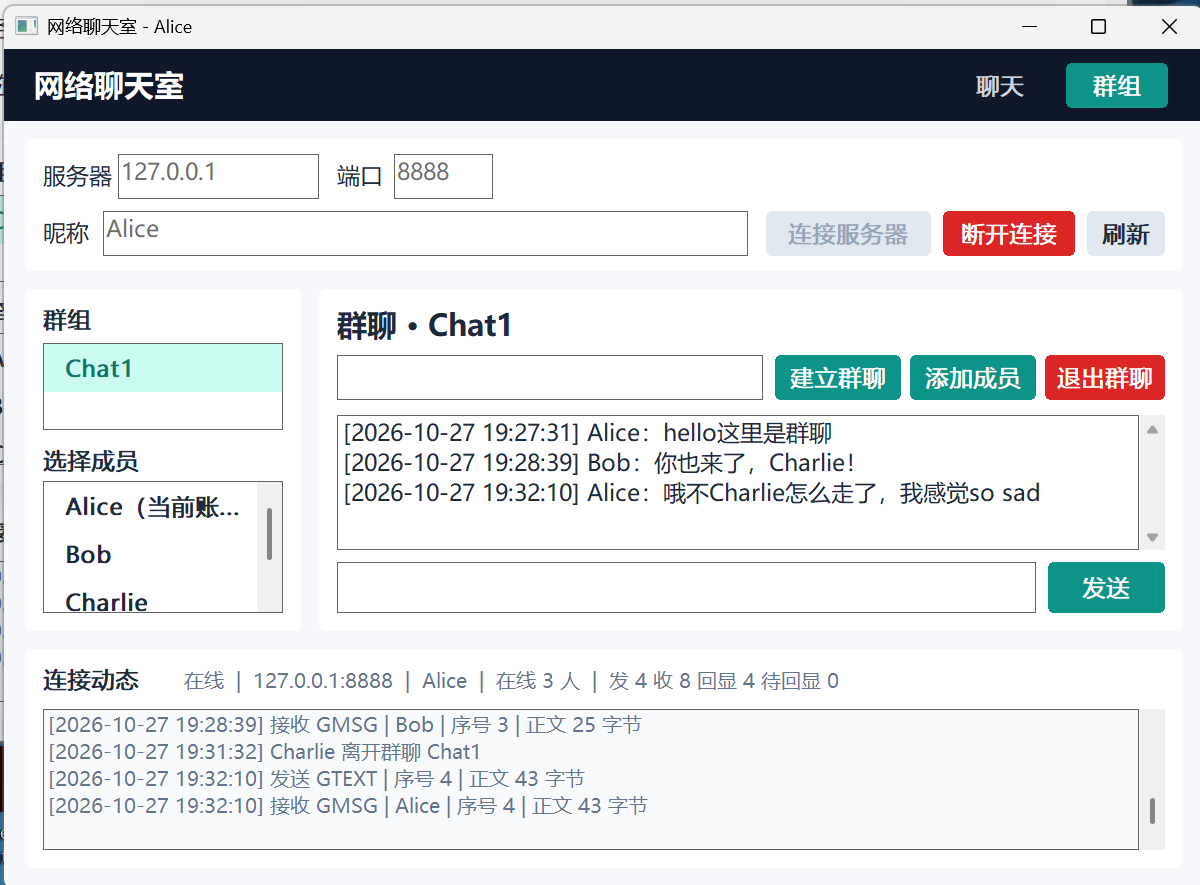
\includegraphics[width=\linewidth,height=10.0cm,keepaspectratio]{images/screen_33.png}
\captionof{figure}{Alice 收到退群通知并继续发言}\label{fig:s33}
\par\smallskip{\raggedright\setlength{\parindent}{2em}\indent Alice 中出现 Charlie 的退群通知，随后又发送了一条新的群消息。\par}
\end{minipage}\par\smallskip
\par\smallskip\noindent\begin{minipage}{\linewidth}\centering
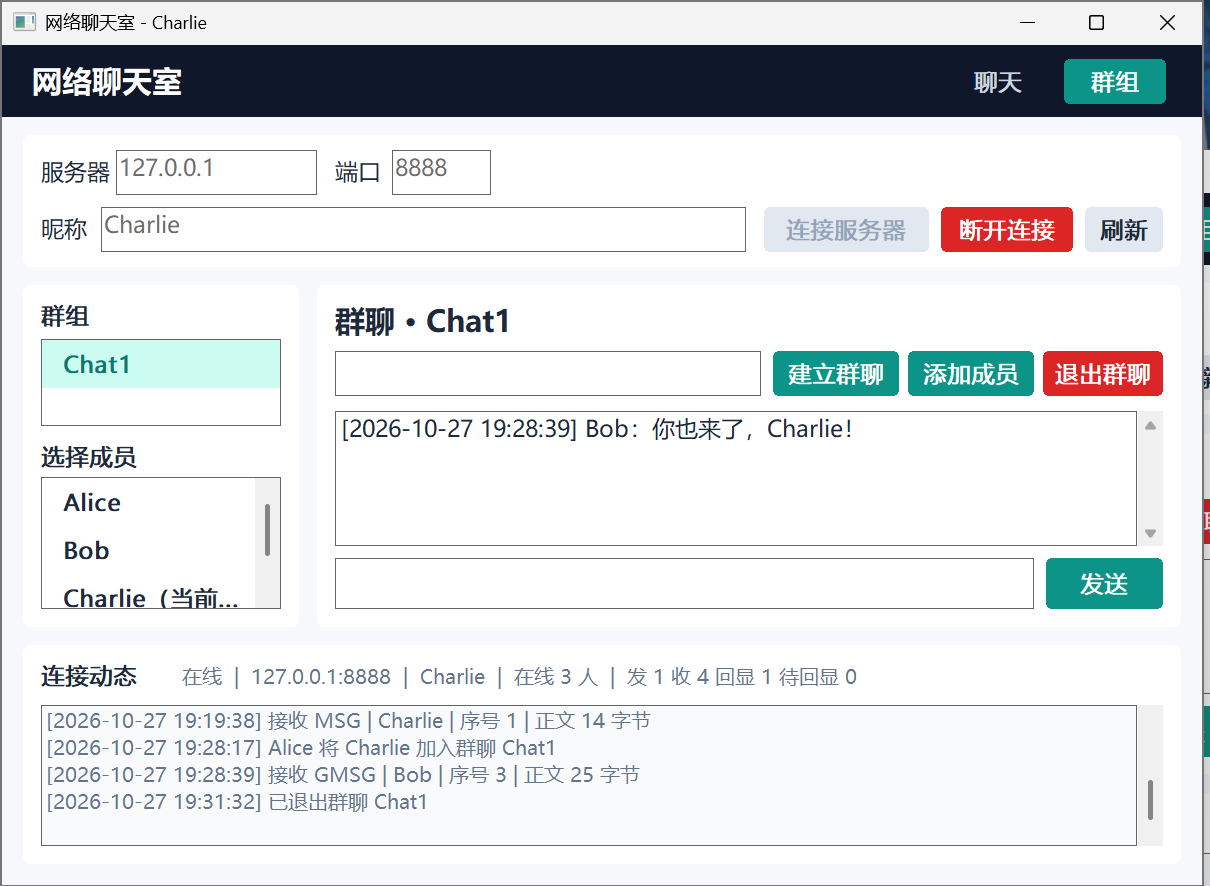
\includegraphics[width=\linewidth,height=10.0cm,keepaspectratio]{images/screen_34.png}
\captionof{figure}{Charlie 退群后的历史}\label{fig:s34}
\par\smallskip{\raggedright\setlength{\parindent}{2em}\indent Charlie 的聊天记录仍停在退出前，接收数保持为 4。\par}
\end{minipage}\par\smallskip
\par\smallskip\noindent\begin{minipage}{\linewidth}\centering
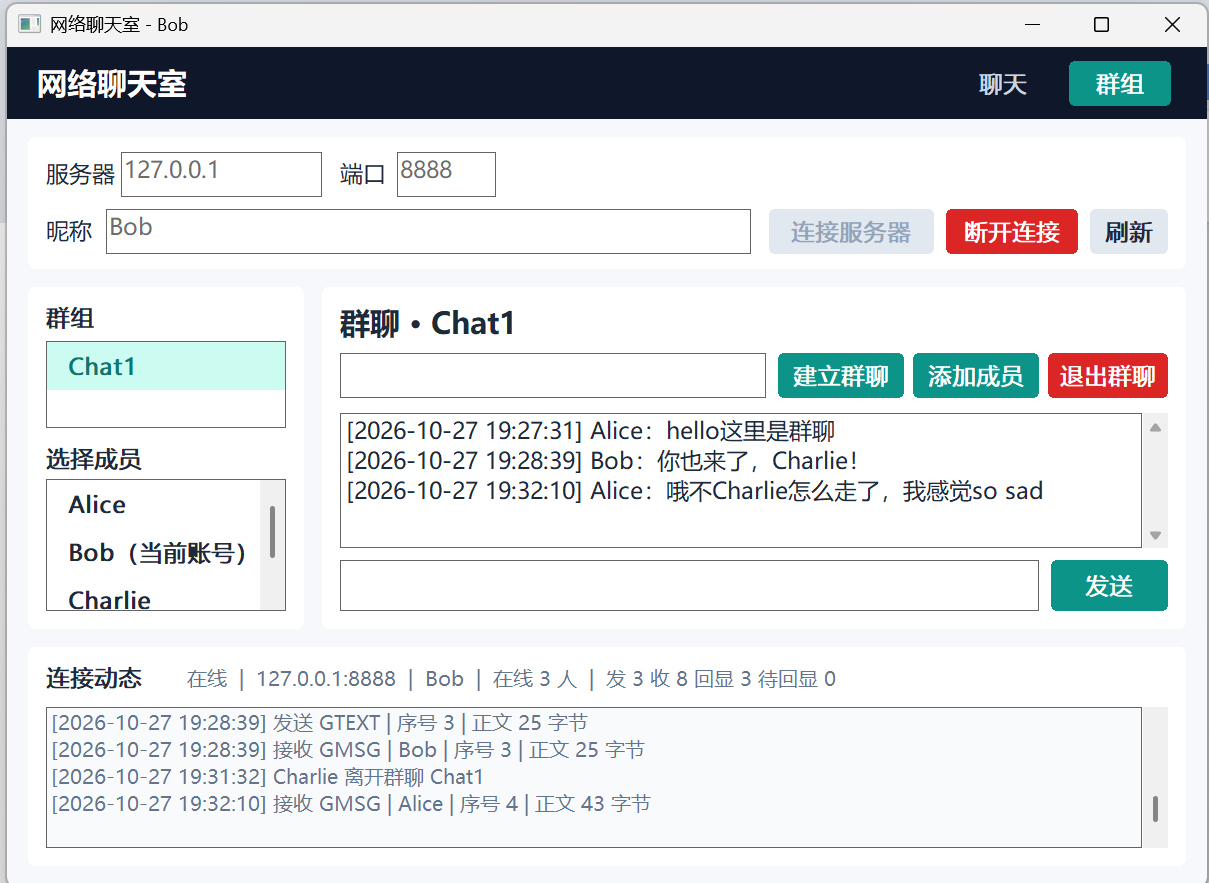
\includegraphics[width=\linewidth,height=10.0cm,keepaspectratio]{images/screen_35.png}
\captionof{figure}{Bob 收到新的群消息}\label{fig:s35}
\par\smallskip{\raggedright\setlength{\parindent}{2em}\indent Bob 收到了 Alice 新发送的群消息，同退群用户的页面形成对照。\par}
\end{minipage}\par\smallskip
Bob 收到了新的群正文，Charlie 则保留退出前的历史，接收数仍为 4，说明退群后已从后续转发集合中移除。

\subsection{成员身份校验}
Charlie 退群后仍在保留的页面中输入并发送群消息，动态区出现 NOT\_MEMBER，表示请求因成员身份被拒绝；与此同时，待回显数变为 1，这个显示现象在后面的错误处理分析中说明。

\par\smallskip\noindent\begin{minipage}{\linewidth}\centering
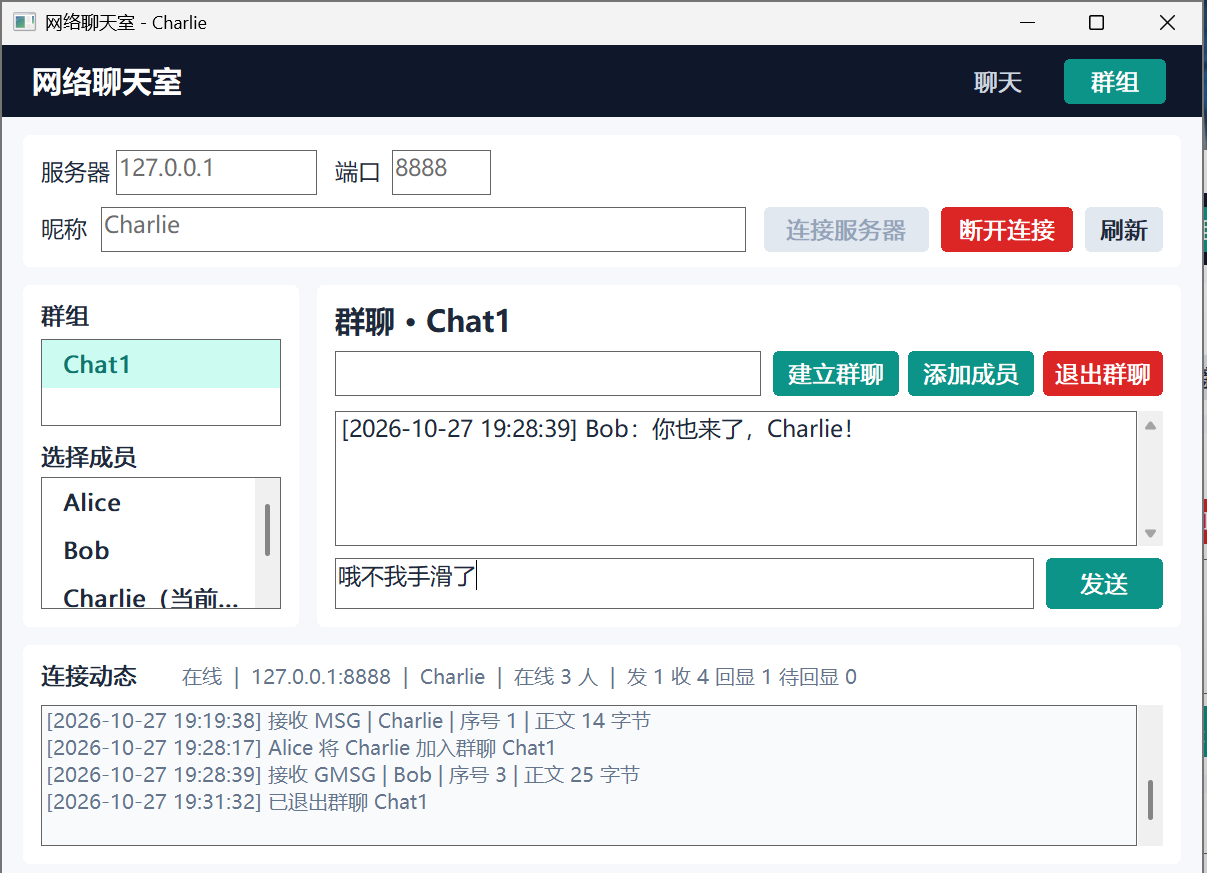
\includegraphics[width=\linewidth,height=10.0cm,keepaspectratio]{images/screen_36.png}
\captionof{figure}{退群后输入的群正文}\label{fig:s36}
\par\smallskip{\raggedright\setlength{\parindent}{2em}\indent Charlie 在保留的群页面输入正文，此时仍处于退群后的状态。\par}
\end{minipage}\par\smallskip
\par\smallskip\noindent\begin{minipage}{\linewidth}\centering
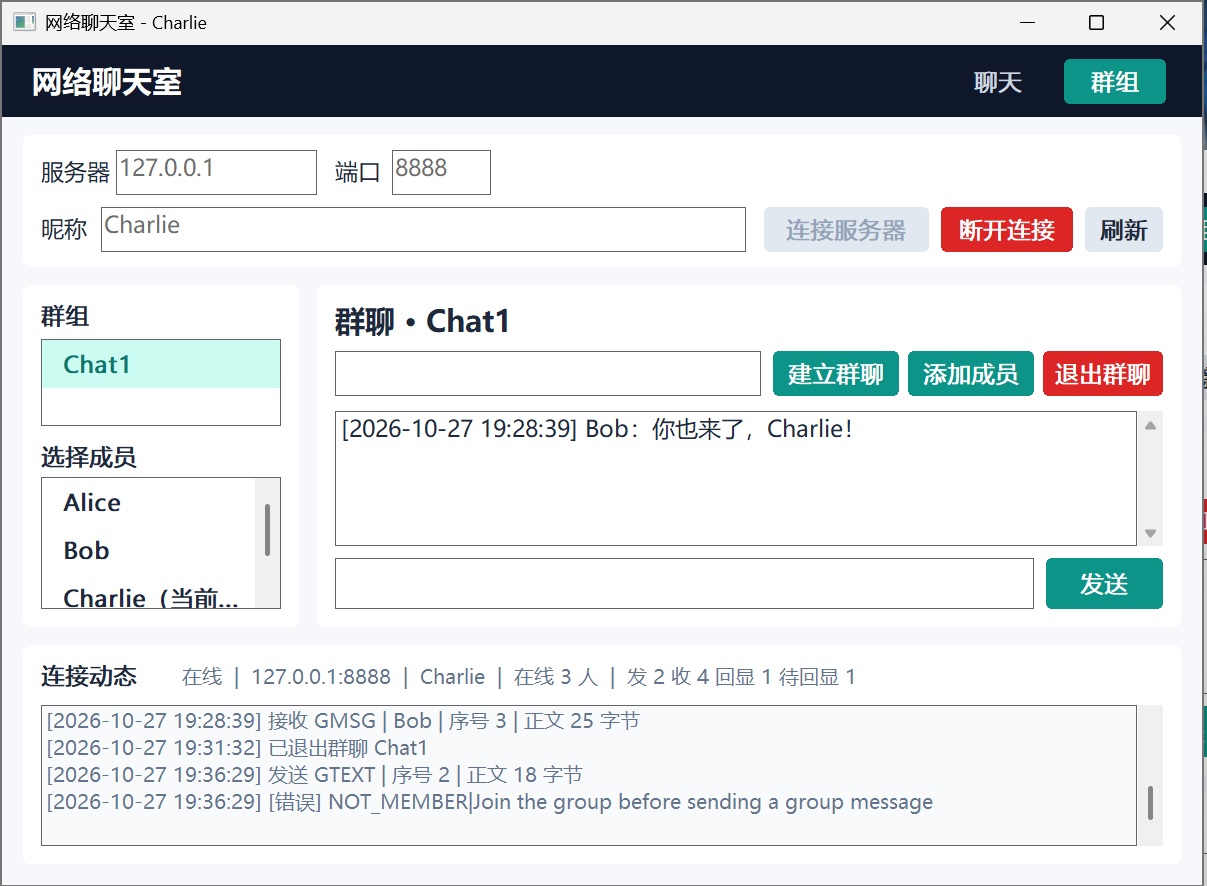
\includegraphics[width=\linewidth,height=10.0cm,keepaspectratio]{images/screen_37.png}
\captionof{figure}{NOT\_MEMBER 错误提示}\label{fig:s37}
\par\smallskip{\raggedright\setlength{\parindent}{2em}\indent 点击发送后显示 NOT\_MEMBER，表明服务器拒绝了该请求；同时待回显数为 1，留下了需要分析的计数现象。\par}
\end{minipage}\par\smallskip
\subsection{重新入群}
在 Alice 中重新添加 Charlie 后继续发言，Charlie 再次收到群消息，并能够向群内回复，Alice、Bob 中也都出现了这一回复。

\par\smallskip\noindent\begin{minipage}{\linewidth}\centering
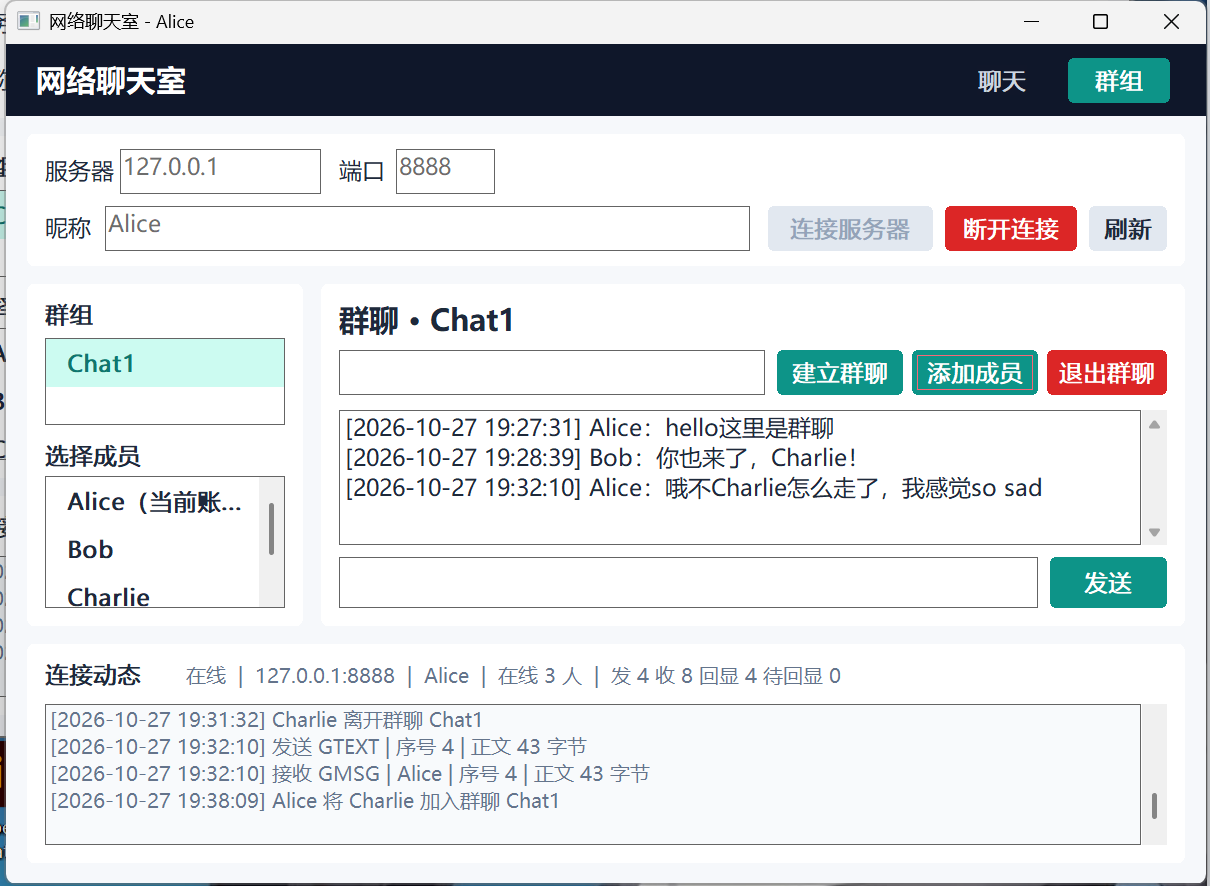
\includegraphics[width=\linewidth,height=10.0cm,keepaspectratio]{images/screen_38.png}
\captionof{figure}{Charlie 再次加入 Chat1}\label{fig:s38}
\par\smallskip{\raggedright\setlength{\parindent}{2em}\indent Alice 重新添加 Charlie 后，动态区再次出现 Charlie 入群提示。\par}
\end{minipage}\par\smallskip
\par\smallskip\noindent\begin{minipage}{\linewidth}\centering
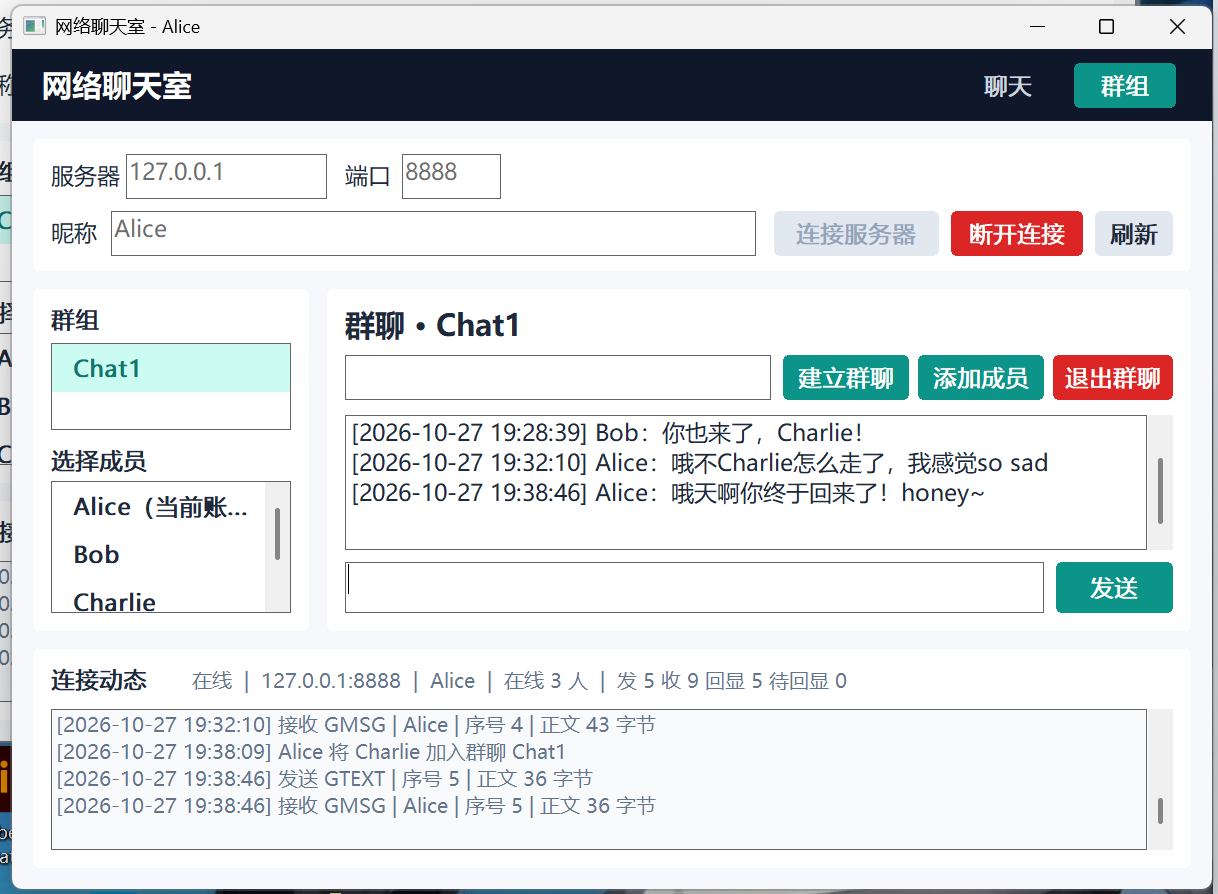
\includegraphics[width=\linewidth,height=10.0cm,keepaspectratio]{images/screen_39.png}
\captionof{figure}{Alice 在成员重新加入后发言}\label{fig:s39}
\par\smallskip{\raggedright\setlength{\parindent}{2em}\indent Alice 随后发送新的群消息，为重新加入的成员提供后续发言。\par}
\end{minipage}\par\smallskip
\par\smallskip\noindent\begin{minipage}{\linewidth}\centering
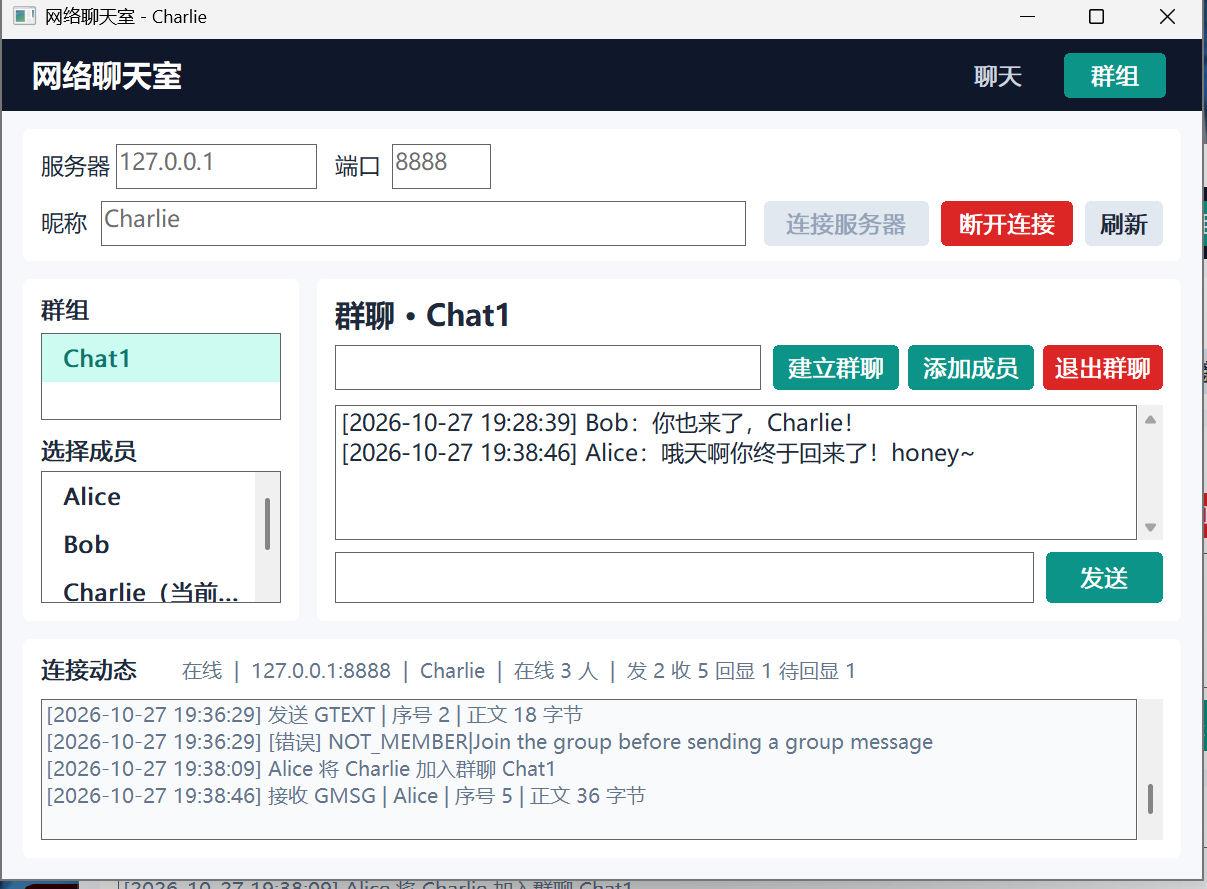
\includegraphics[width=\linewidth,height=10.0cm,keepaspectratio]{images/screen_40.png}
\captionof{figure}{Charlie 再次收到群消息}\label{fig:s40}
\par\smallskip{\raggedright\setlength{\parindent}{2em}\indent Charlie 再次收到群正文，而之前被拒绝请求留下的待回显数仍为 1。\par}
\end{minipage}\par\smallskip
\par\smallskip\noindent\begin{minipage}{\linewidth}\centering
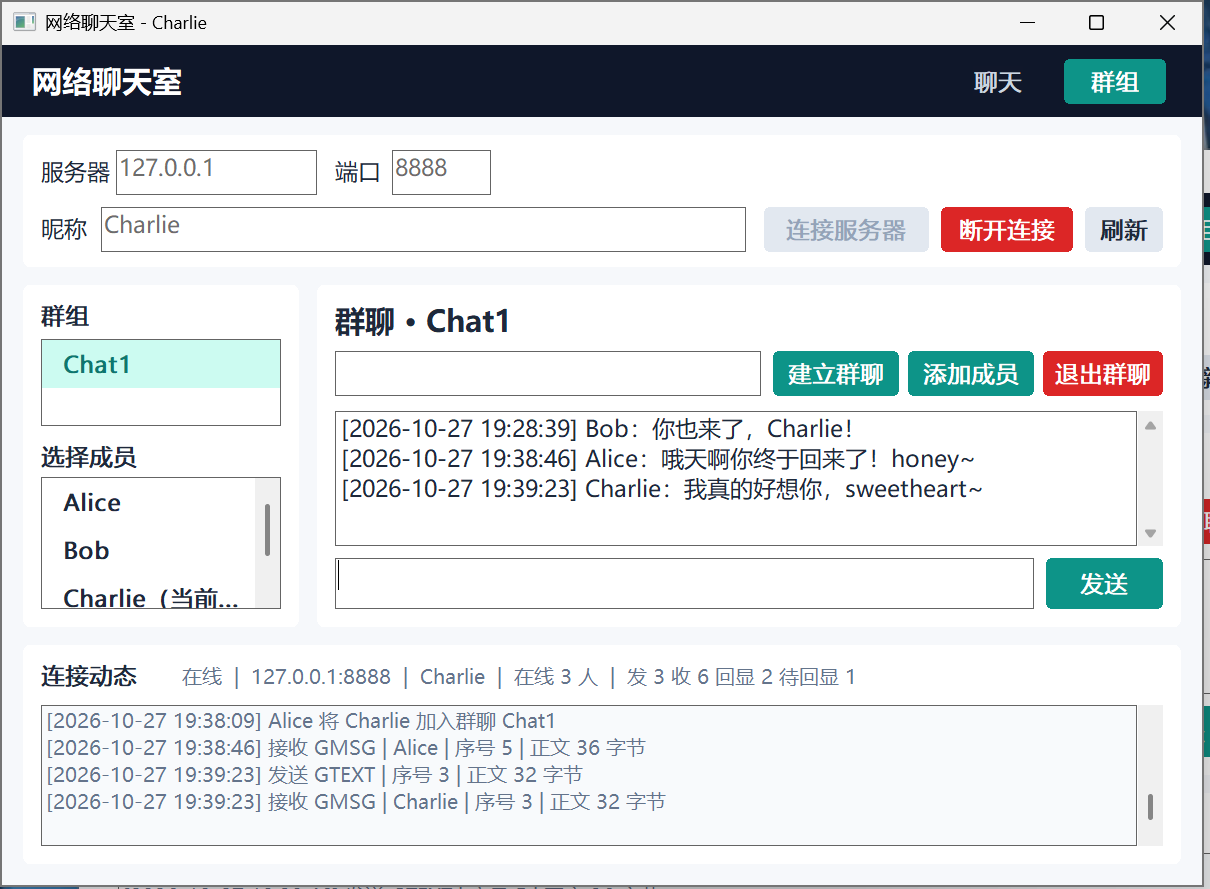
\includegraphics[width=\linewidth,height=10.0cm,keepaspectratio]{images/screen_41.png}
\captionof{figure}{Charlie 重新入群后的回复}\label{fig:s41}
\par\smallskip{\raggedright\setlength{\parindent}{2em}\indent Charlie 回复后能够收到本人的群消息回显，重新入群后的发送已恢复。\par}
\end{minipage}\par\smallskip
\par\smallskip\noindent\begin{minipage}{\linewidth}\centering
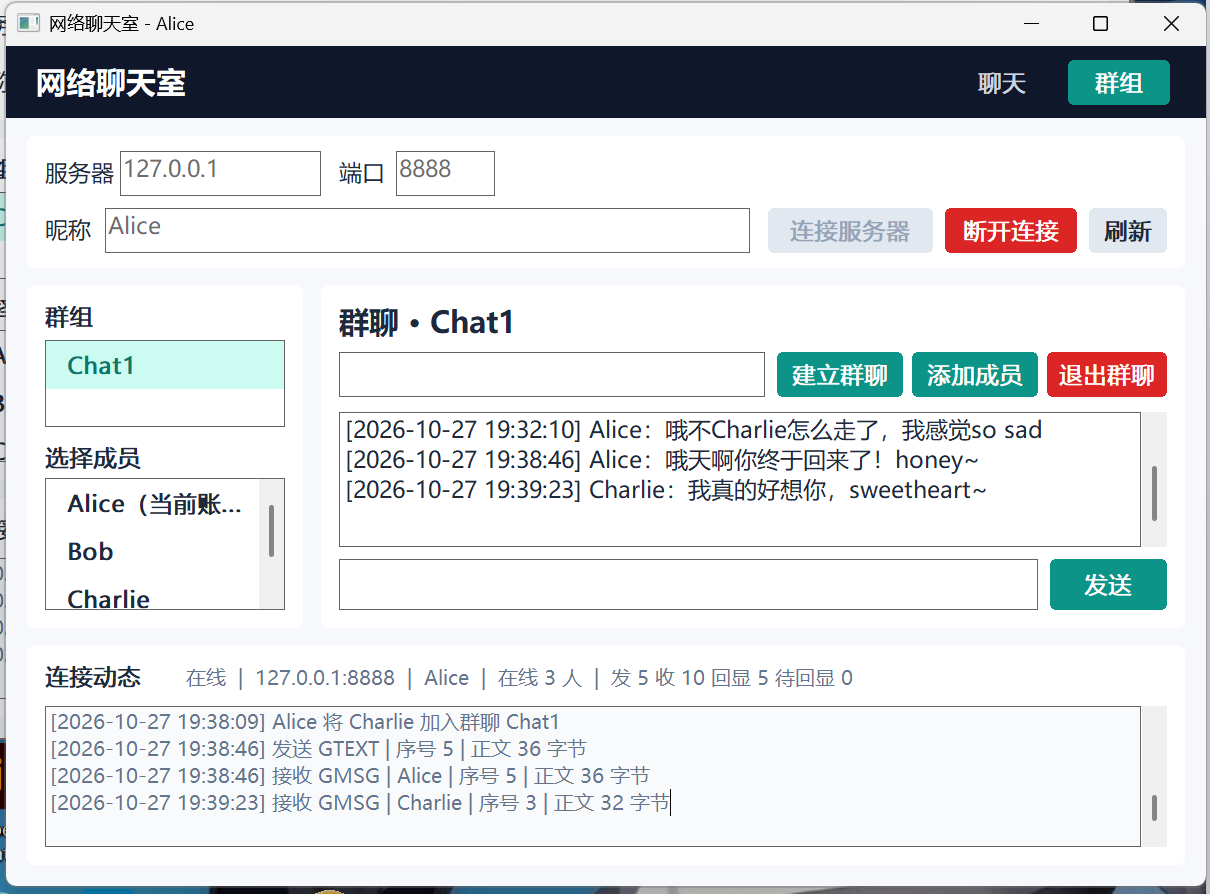
\includegraphics[width=\linewidth,height=10.0cm,keepaspectratio]{images/screen_42.png}
\captionof{figure}{Alice 收到 Charlie 的群回复}\label{fig:s42}
\par\smallskip{\raggedright\setlength{\parindent}{2em}\indent Alice 收到 Charlie 的回复，新的发言已经转发到原成员的连接。\par}
\end{minipage}\par\smallskip
\par\smallskip\noindent\begin{minipage}{\linewidth}\centering
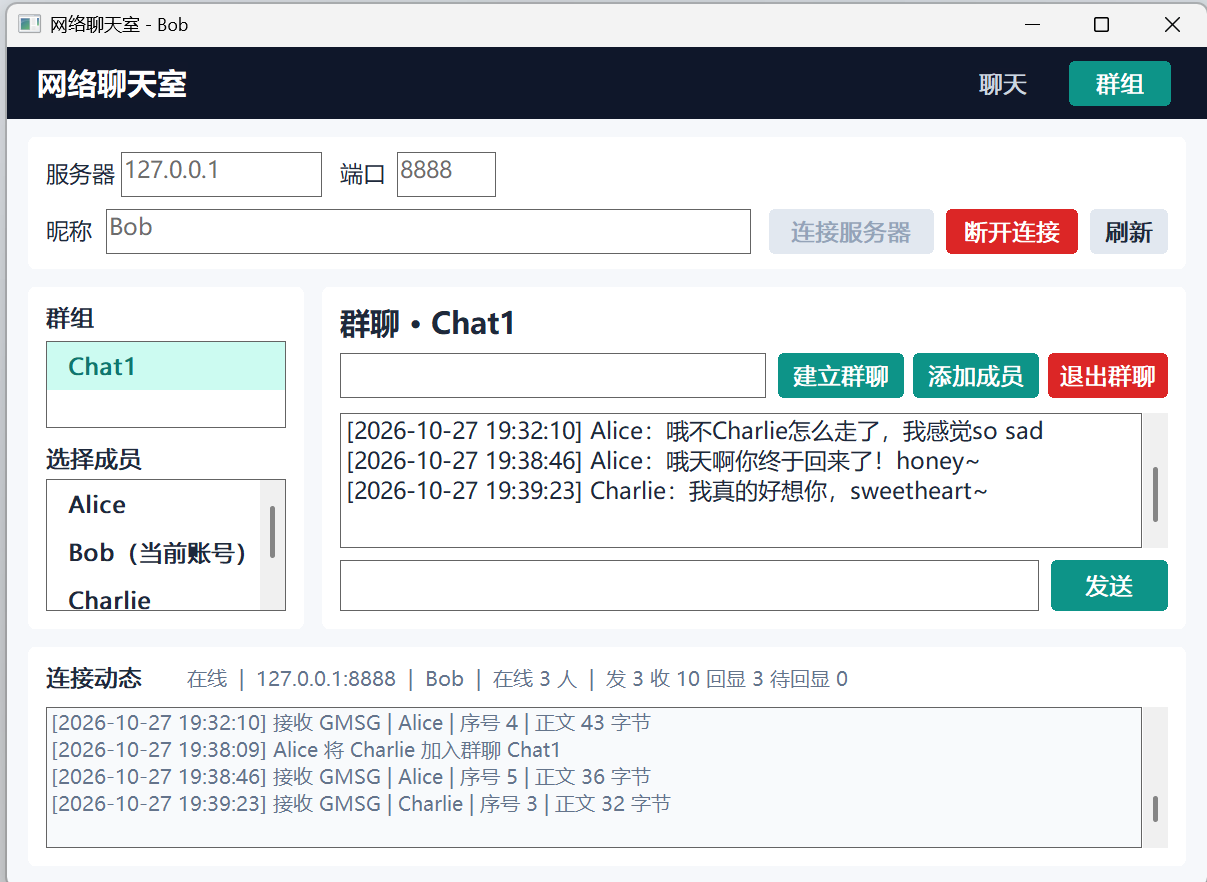
\includegraphics[width=\linewidth,height=10.0cm,keepaspectratio]{images/screen_43.png}
\captionof{figure}{Bob 收到 Charlie 的群回复}\label{fig:s43}
\par\smallskip{\raggedright\setlength{\parindent}{2em}\indent Bob 中也出现相同回复，三位群成员都已经接收到这条消息。\par}
\end{minipage}\par\smallskip
重新入群后的合法消息已经收到回显，先前被拒绝请求留下的待回显 1 仍在界面中，因此需要将实际收发结果和这一遗留计数分开理解。

\subsection{断开重连}
Bob 主动断开时，底部依次出现 QUIT、退出确认和离线提示；服务器及另外两位用户继续运行，随后使用原昵称重新连接。

重新登录后，在线人数恢复为 3，Bob 的计数从新会话开始。接着 Bob 发送公共消息、Charlie 回复，两个方向的消息都出现在对应窗口中。

\par\smallskip\noindent\begin{minipage}{\linewidth}\centering
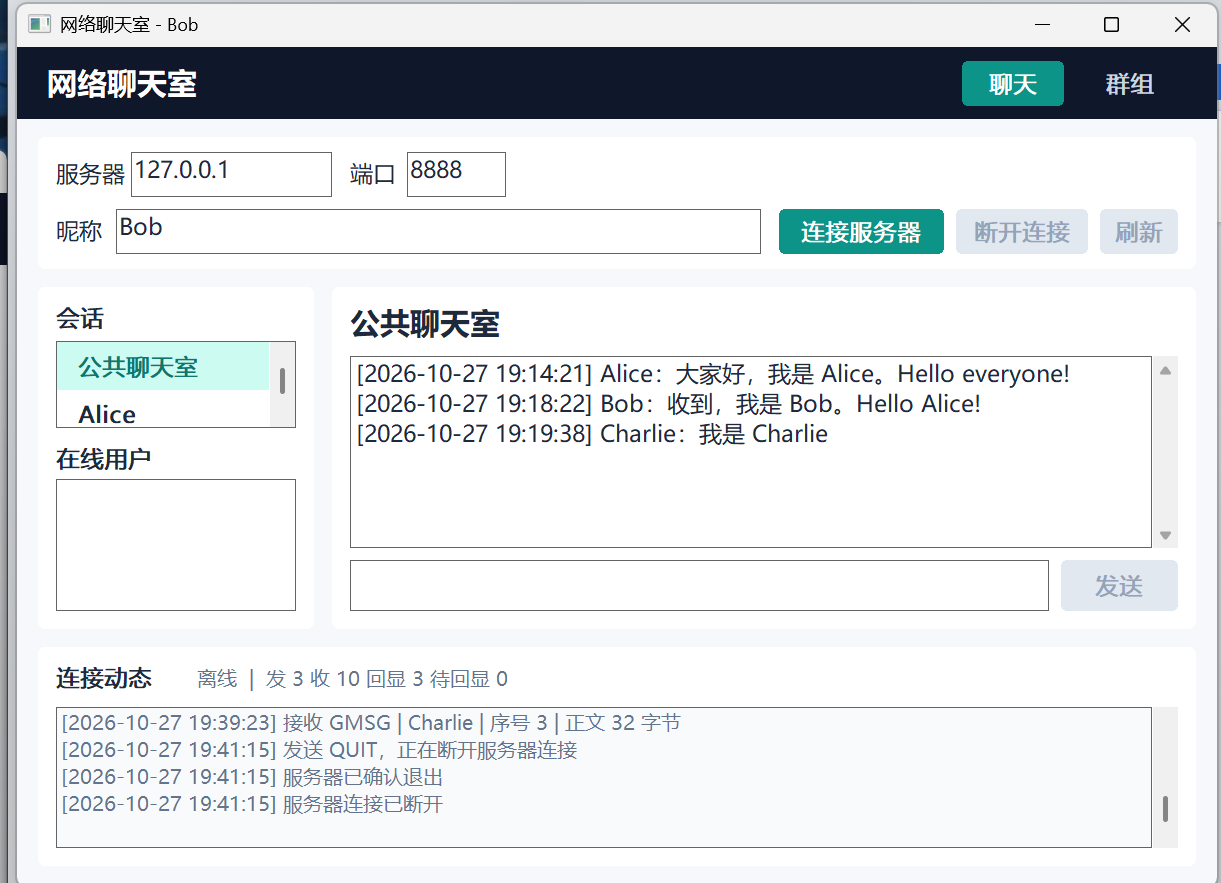
\includegraphics[width=\linewidth,height=10.0cm,keepaspectratio]{images/screen_44.png}
\captionof{figure}{Bob 主动断开连接}\label{fig:s44}
\par\smallskip{\raggedright\setlength{\parindent}{2em}\indent Bob 点击断开后，下方依次显示 QUIT、退出确认和连接断开，页面回到离线状态。\par}
\end{minipage}\par\smallskip
\par\smallskip\noindent\begin{minipage}{\linewidth}\centering
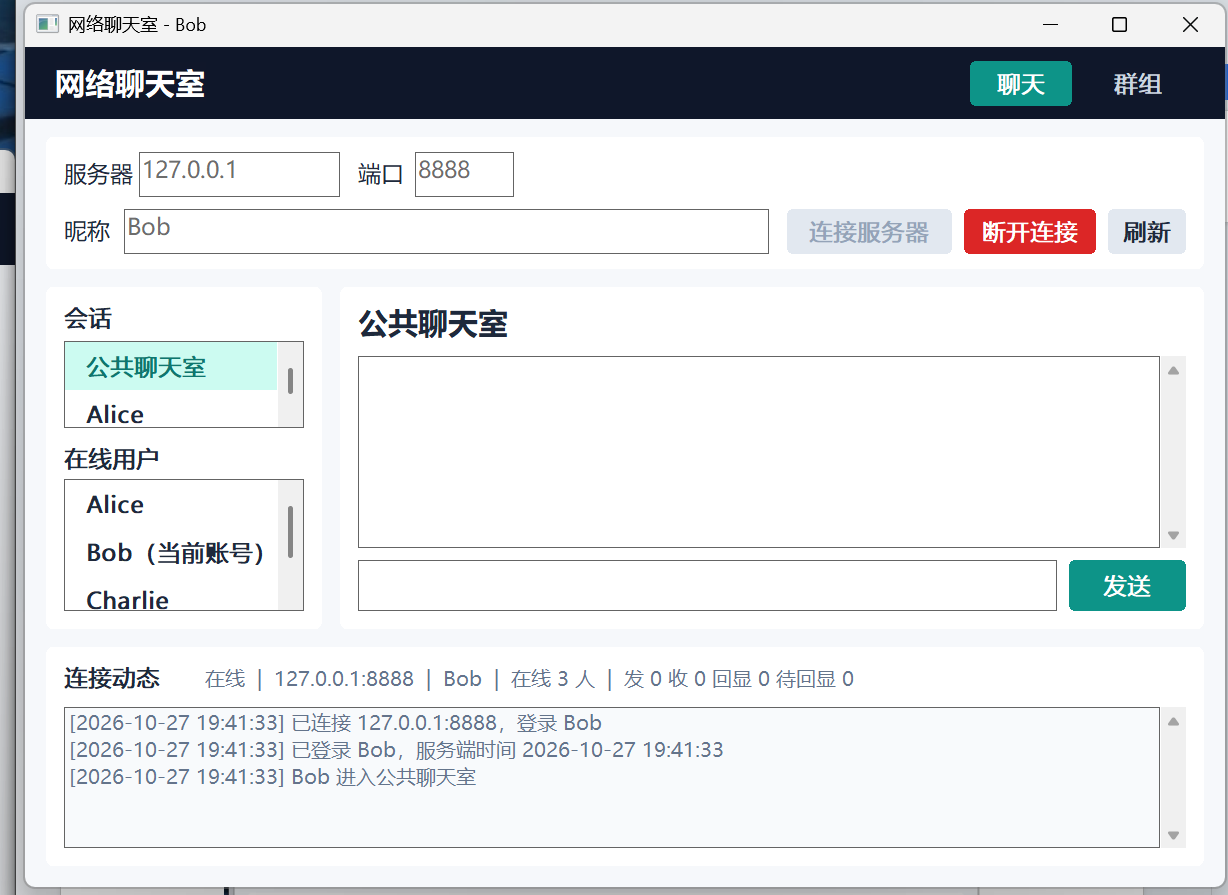
\includegraphics[width=\linewidth,height=10.0cm,keepaspectratio]{images/screen_45.png}
\captionof{figure}{Bob 使用原昵称重连}\label{fig:s45}
\par\smallskip{\raggedright\setlength{\parindent}{2em}\indent 使用原昵称 Bob 重连后，在线人数恢复为 3，收发计数从新会话开始。\par}
\end{minipage}\par\smallskip
\par\smallskip\noindent\begin{minipage}{\linewidth}\centering
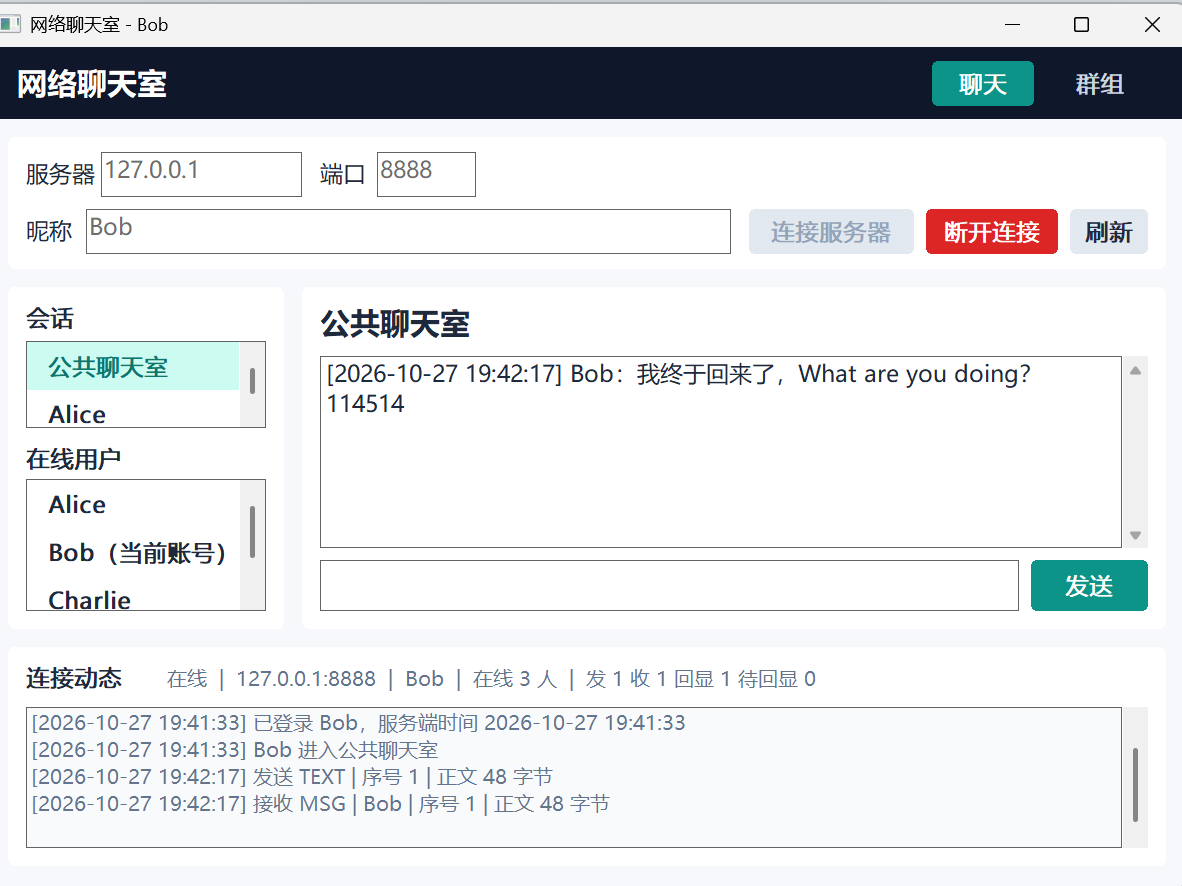
\includegraphics[width=\linewidth,height=10.0cm,keepaspectratio]{images/screen_46.png}
\captionof{figure}{Bob 重连后的公共发言}\label{fig:s46}
\par\smallskip{\raggedright\setlength{\parindent}{2em}\indent Bob 在新连接中发送中英文消息，公共会话出现本人回显。\par}
\end{minipage}\par\smallskip
\par\smallskip\noindent\begin{minipage}{\linewidth}\centering
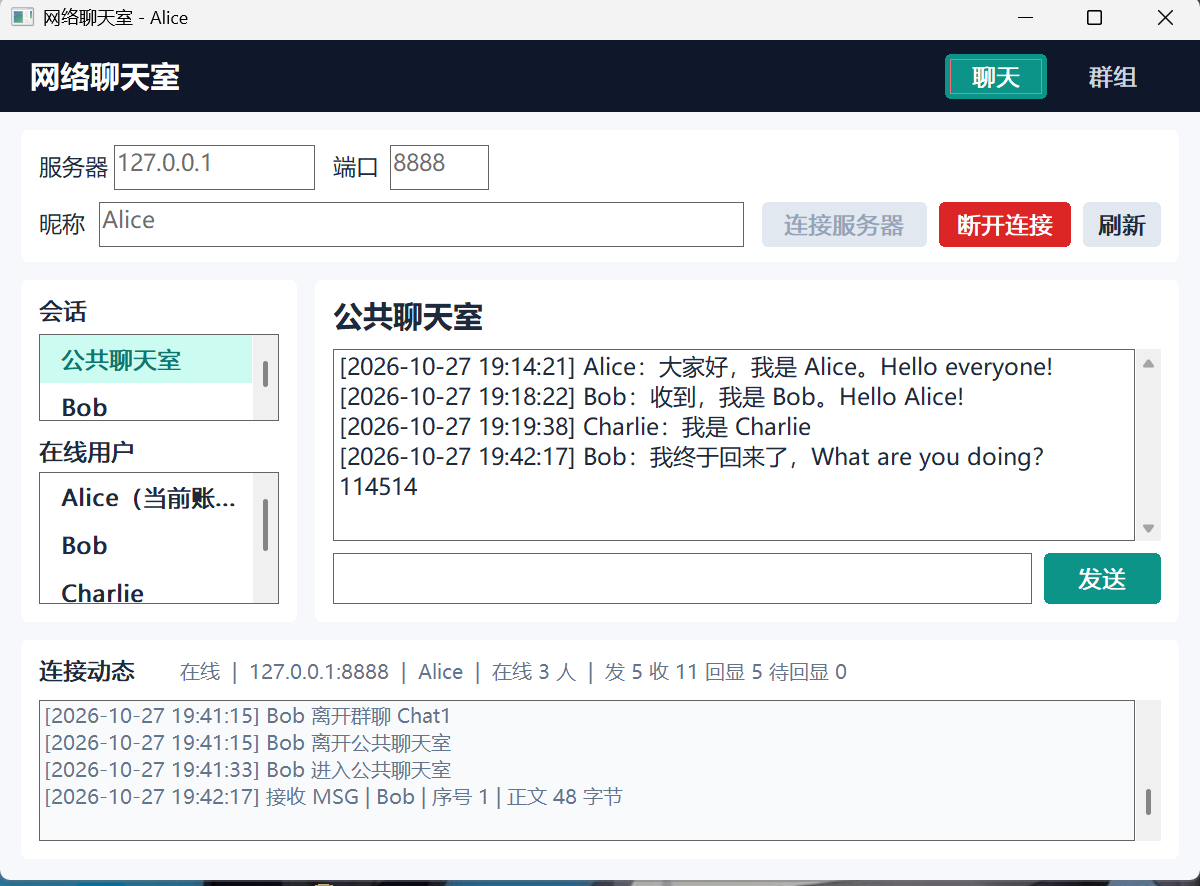
\includegraphics[width=\linewidth,height=10.0cm,keepaspectratio]{images/screen_47.png}
\captionof{figure}{Alice 中的 Bob 重连记录}\label{fig:s47}
\par\smallskip{\raggedright\setlength{\parindent}{2em}\indent Alice 的动态保留 Bob 离开及重新进入的记录，聊天区同时出现重连后的新发言。\par}
\end{minipage}\par\smallskip
\par\smallskip\noindent\begin{minipage}{\linewidth}\centering
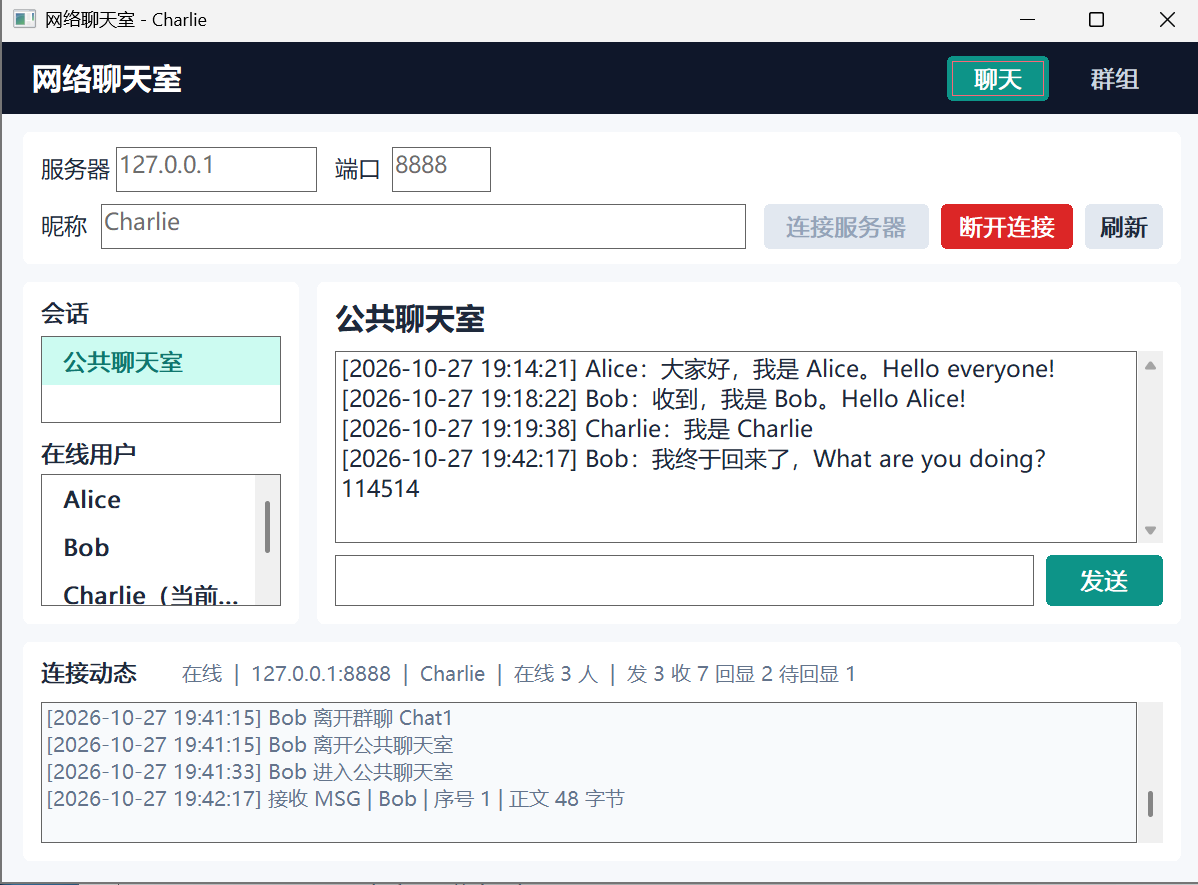
\includegraphics[width=\linewidth,height=10.0cm,keepaspectratio]{images/screen_48.png}
\captionof{figure}{Charlie 收到重连后的消息}\label{fig:s48}
\par\smallskip{\raggedright\setlength{\parindent}{2em}\indent Charlie 也收到了 Bob 的新消息，重连后的公共转发已经送达另一位用户。\par}
\end{minipage}\par\smallskip
\par\smallskip\noindent\begin{minipage}{\linewidth}\centering
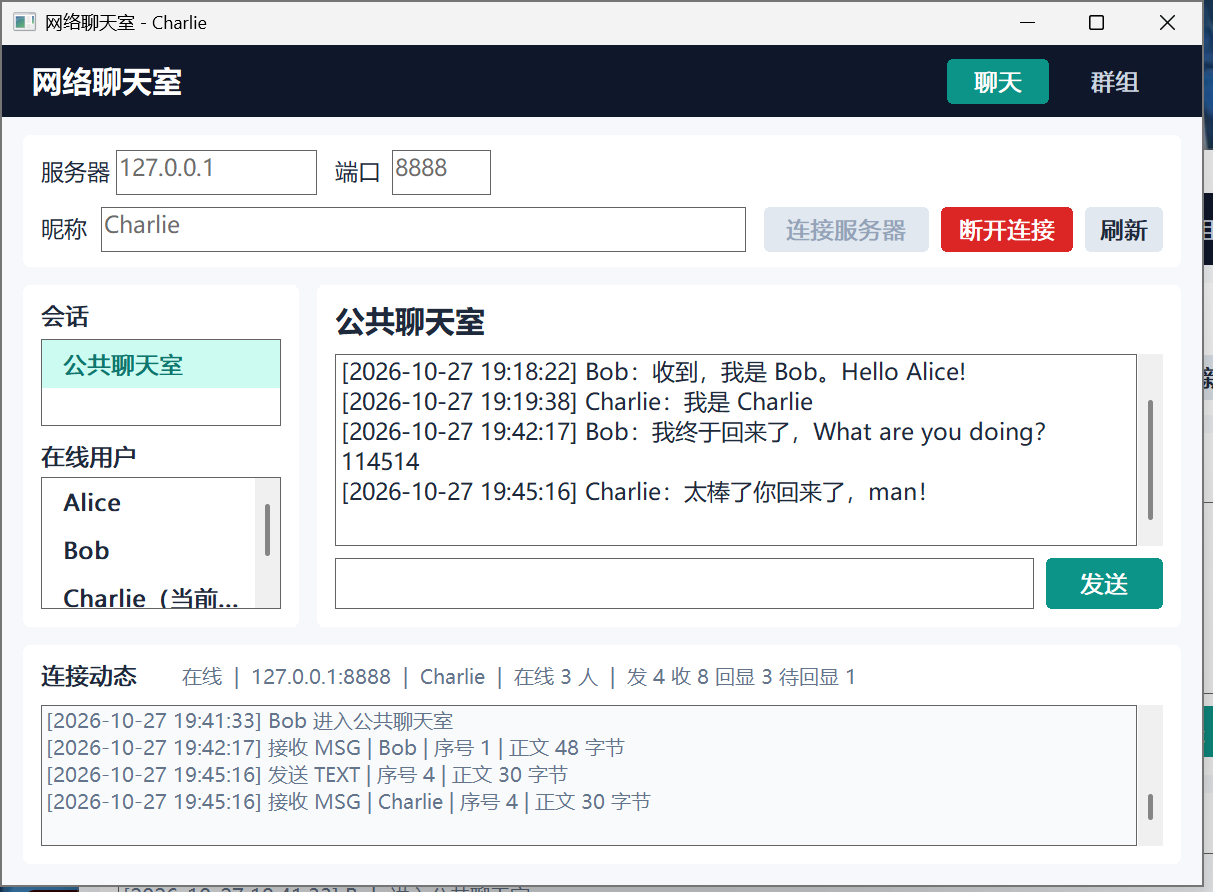
\includegraphics[width=\linewidth,height=10.0cm,keepaspectratio]{images/screen_49.png}
\captionof{figure}{Charlie 回复 Bob}\label{fig:s49}
\par\smallskip{\raggedright\setlength{\parindent}{2em}\indent Charlie 继续回复，消息显示在本人公共会话中，并进入服务器转发过程。\par}
\end{minipage}\par\smallskip
\par\smallskip\noindent\begin{minipage}{\linewidth}\centering
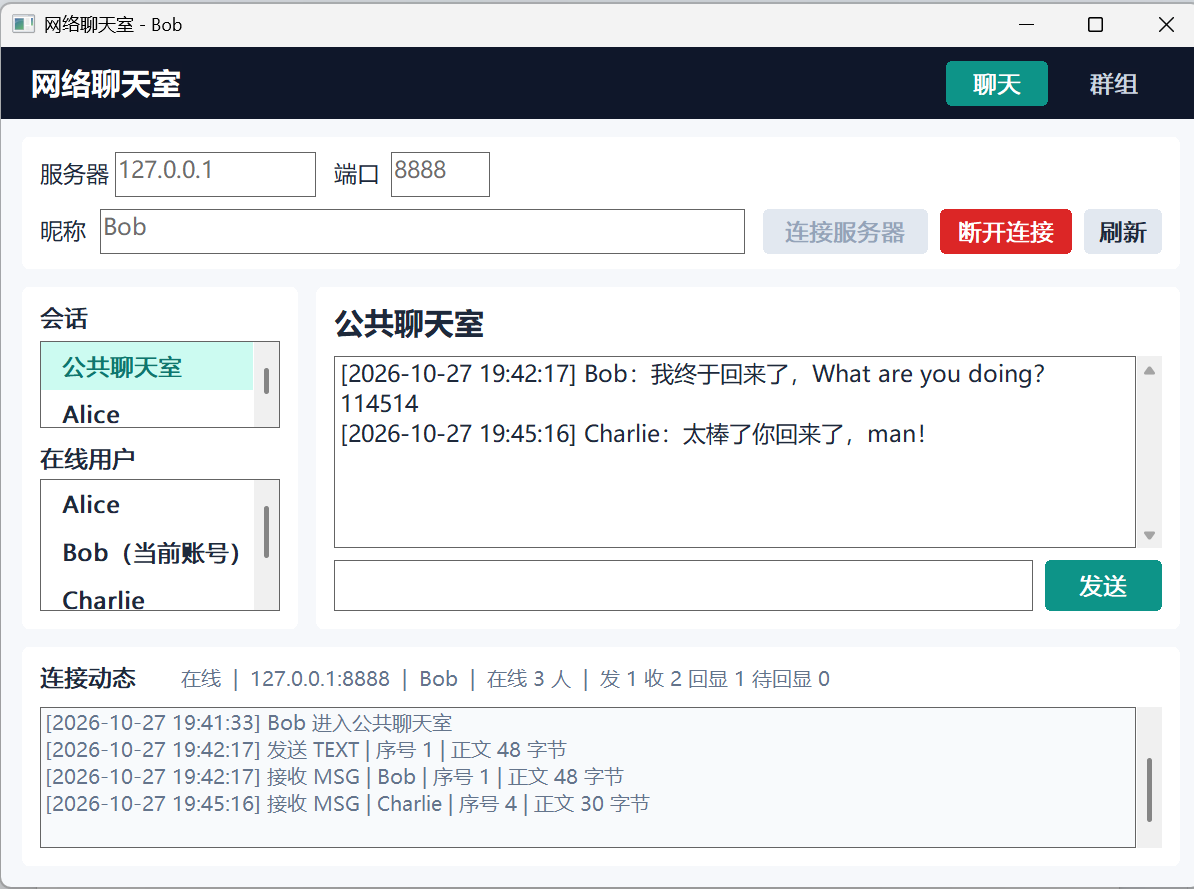
\includegraphics[width=\linewidth,height=10.0cm,keepaspectratio]{images/screen_50.png}
\captionof{figure}{Bob 收到重连后的回复}\label{fig:s50}
\par\smallskip{\raggedright\setlength{\parindent}{2em}\indent Bob 收到 Charlie 的回复，重连后的发送和接收两个方向都已经呈现在记录中。\par}
\end{minipage}\par\smallskip
在 Alice 的动态中可以同时看到 Bob 离开、重新进入及后续发言，Bob 也能够继续收发，说明旧会话结束后已经重新建立并登记了连接。

\subsection{窗口缩放}
将 Charlie 窗口先横向拉宽，再调为较窄、较高的形状，聊天区、输入框、发送按钮和动态区随客户区尺寸重新排列，两种状态如下图。

\par\smallskip\noindent\begin{minipage}{\linewidth}\centering
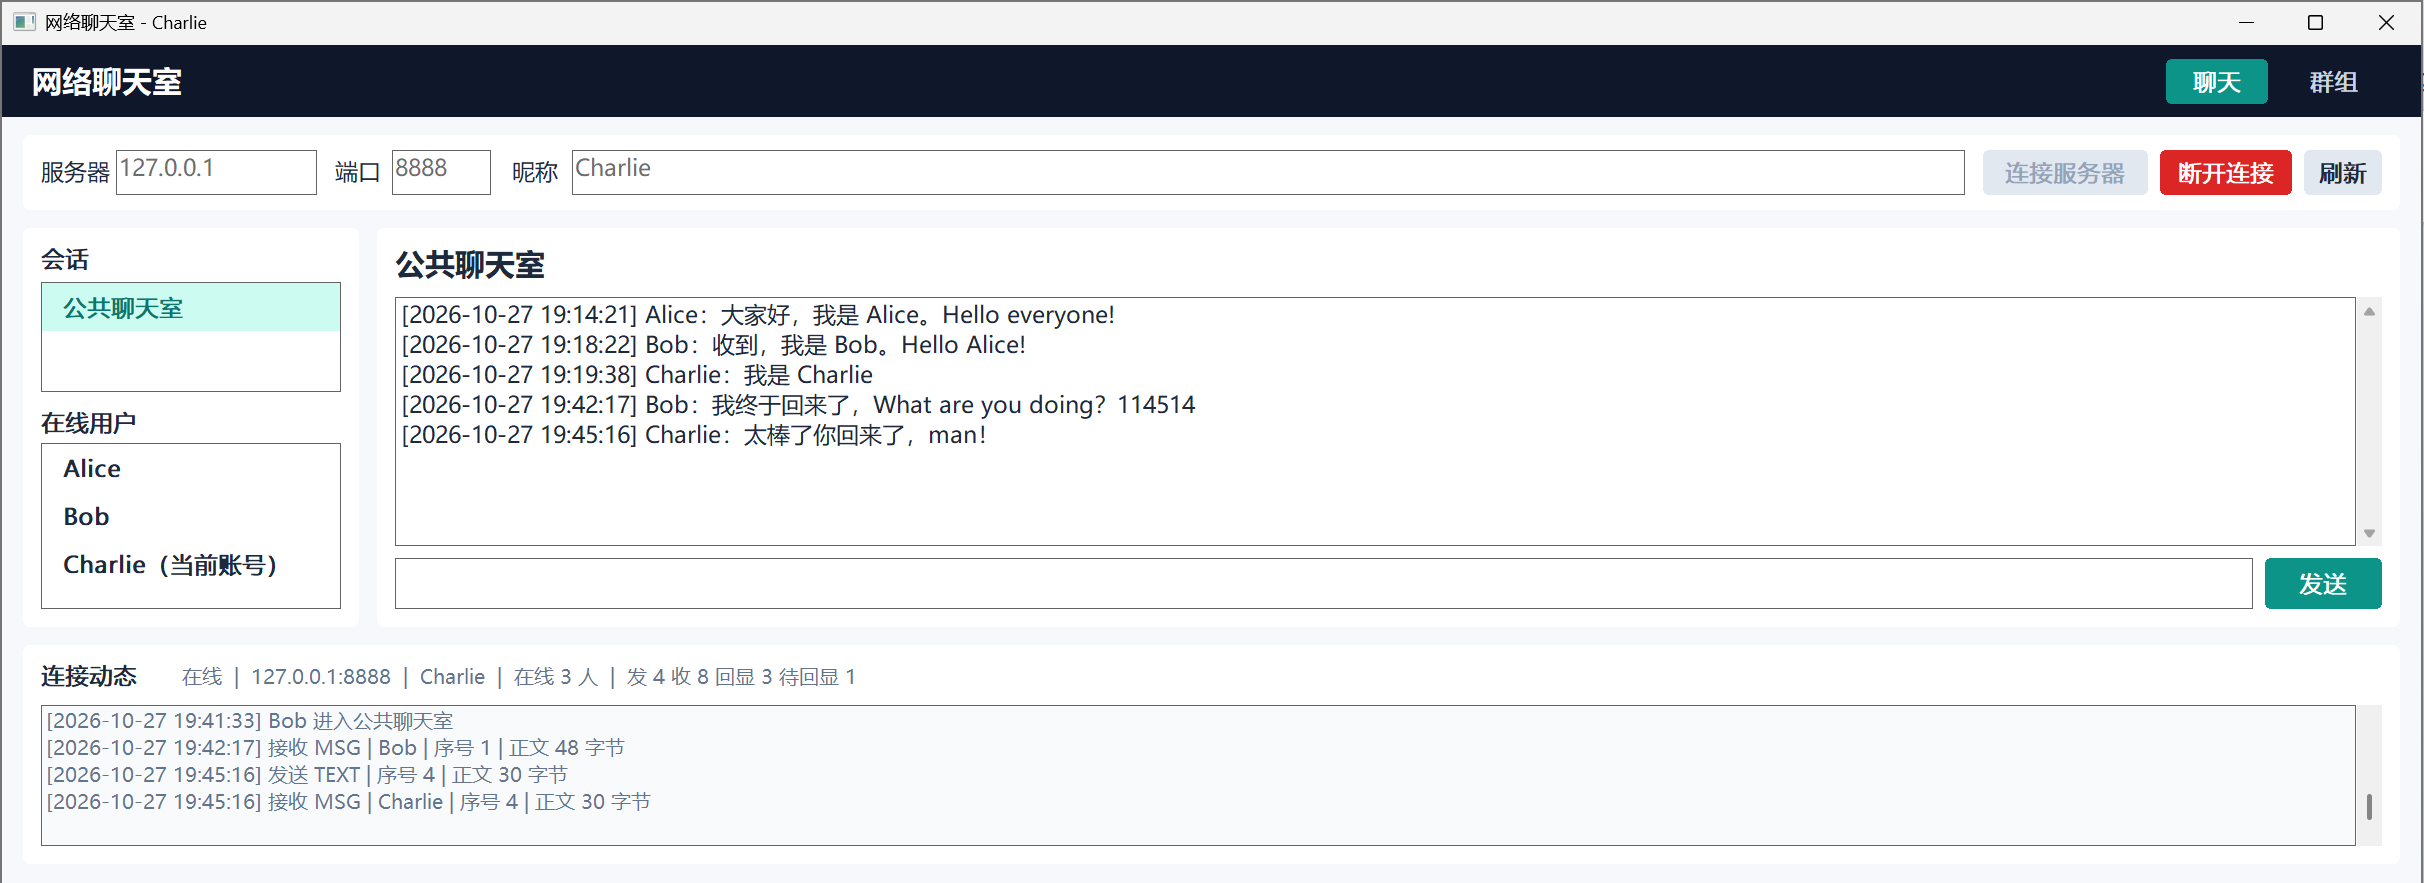
\includegraphics[width=\linewidth,height=10.0cm,keepaspectratio]{images/screen_51.png}
\captionof{figure}{横向拉宽后的窗口}\label{fig:s51}
\par\smallskip{\raggedright\setlength{\parindent}{2em}\indent 横向拉宽窗口后，聊天区和底部动态随之展开，输入框及发送按钮保持相邻。\par}
\end{minipage}\par\smallskip
\par\smallskip\noindent\begin{minipage}{\linewidth}\centering
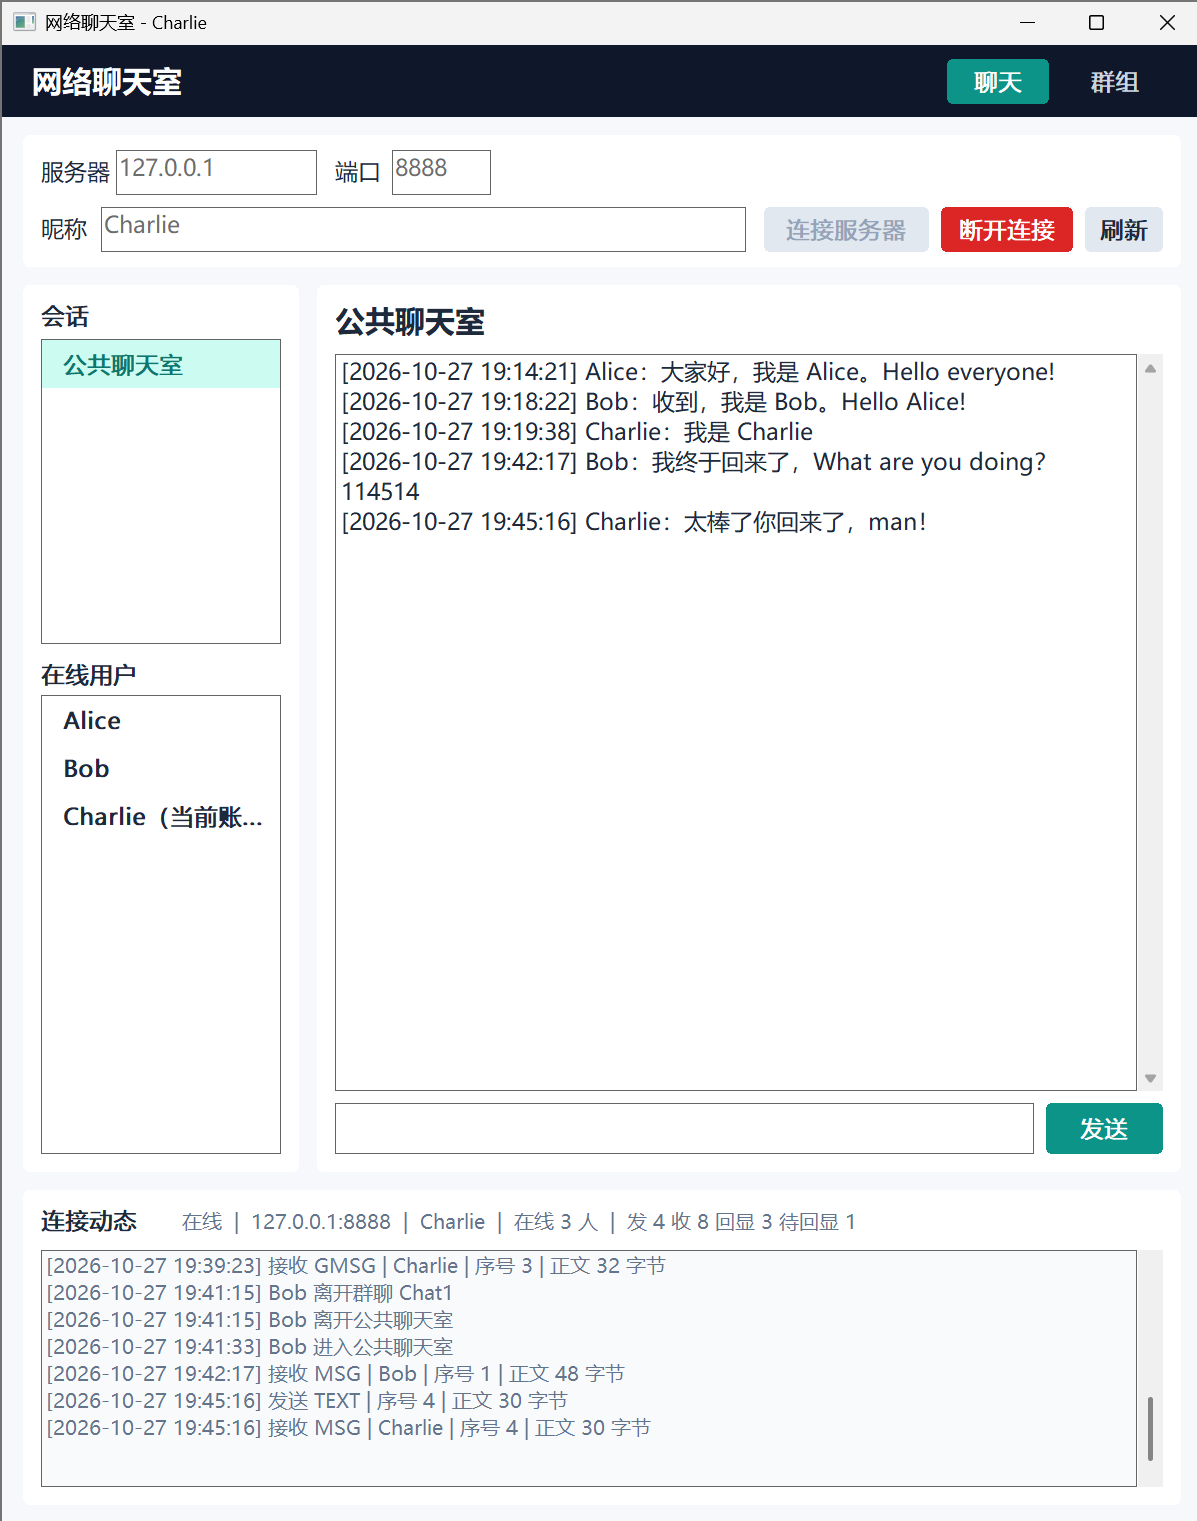
\includegraphics[width=\linewidth,height=10.0cm,keepaspectratio]{images/screen_52.png}
\captionof{figure}{较窄较高的窗口}\label{fig:s52}
\par\smallskip{\raggedright\setlength{\parindent}{2em}\indent 将窗口调窄并拉高后，输入区和动态区仍完整可见，控件随新的尺寸重新排列。\par}
\end{minipage}\par\smallskip
两种尺寸下都保留了输入和发送区域，底部动态也持续可见，分别对应 WM\_SIZE 中的布局计算及按 DPI 换算后的尺寸。

\subsection{关闭客户端}
关闭 Charlie 前，先记录仍在线的页面；点击右上角关闭后，Alice 的在线名单变为两人，并出现离线通知，随后继续在 Alice、Bob 之间发送公共消息。

\par\smallskip\noindent\begin{minipage}{\linewidth}\centering
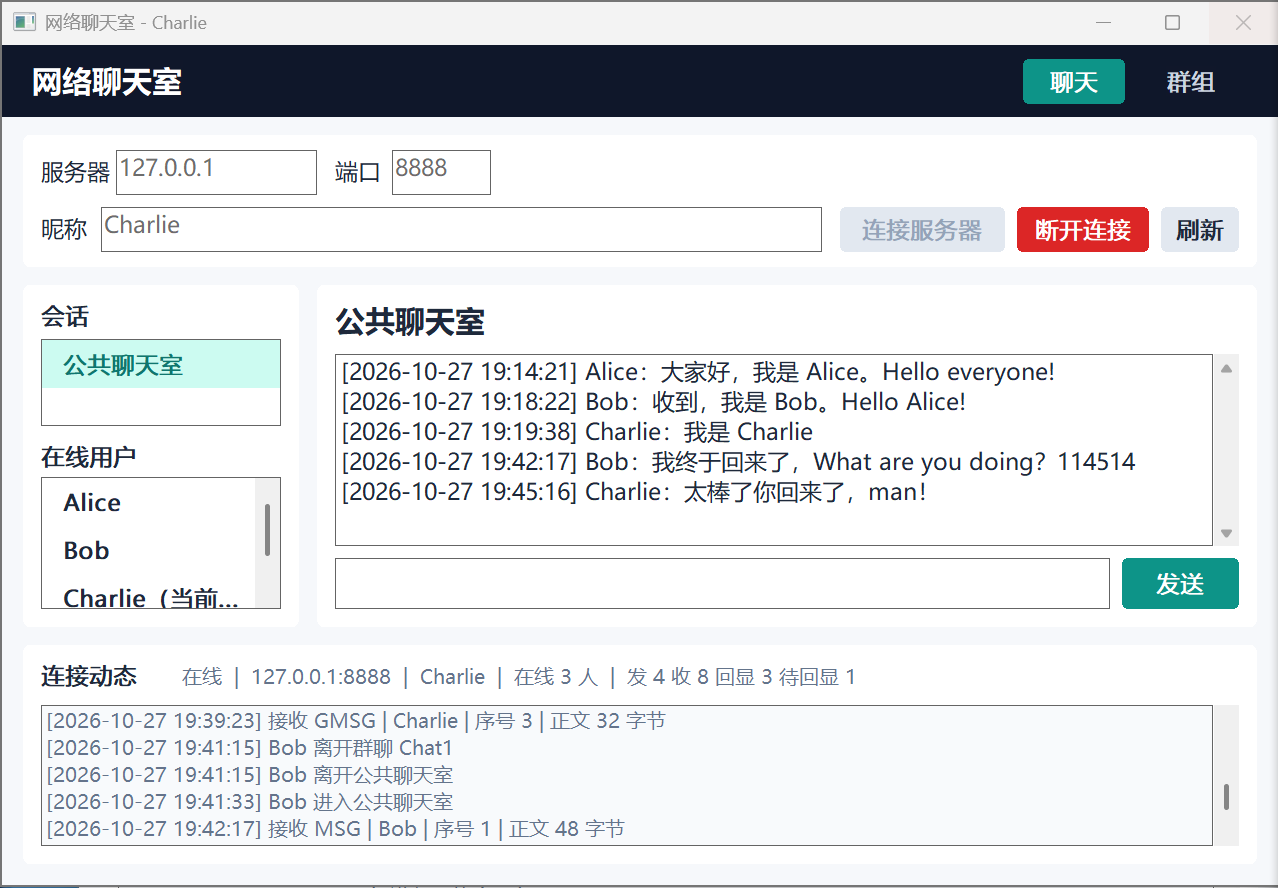
\includegraphics[width=\linewidth,height=10.0cm,keepaspectratio]{images/screen_53.png}
\captionof{figure}{Charlie 关闭前的状态}\label{fig:s53}
\par\smallskip{\raggedright\setlength{\parindent}{2em}\indent 关闭前的 Charlie 窗口仍显示在线，聊天历史和当前计数均保留在页面中。\par}
\end{minipage}\par\smallskip
\par\smallskip\noindent\begin{minipage}{\linewidth}\centering
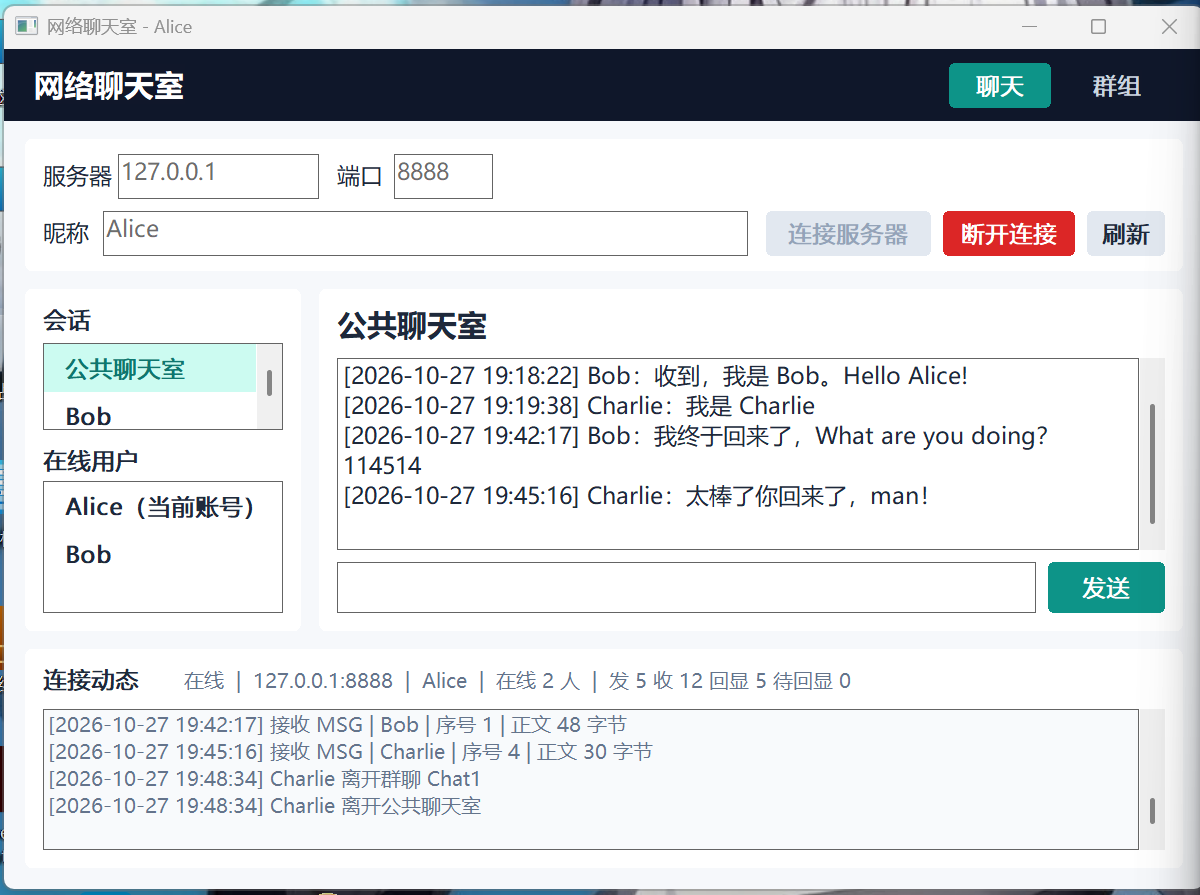
\includegraphics[width=\linewidth,height=10.0cm,keepaspectratio]{images/screen_54.png}
\captionof{figure}{Alice 收到 Charlie 离线通知}\label{fig:s54}
\par\smallskip{\raggedright\setlength{\parindent}{2em}\indent 关闭 Charlie 后，Alice 的名单只剩两人，底部增加 Charlie 离线通知。\par}
\end{minipage}\par\smallskip
\par\smallskip\noindent\begin{minipage}{\linewidth}\centering
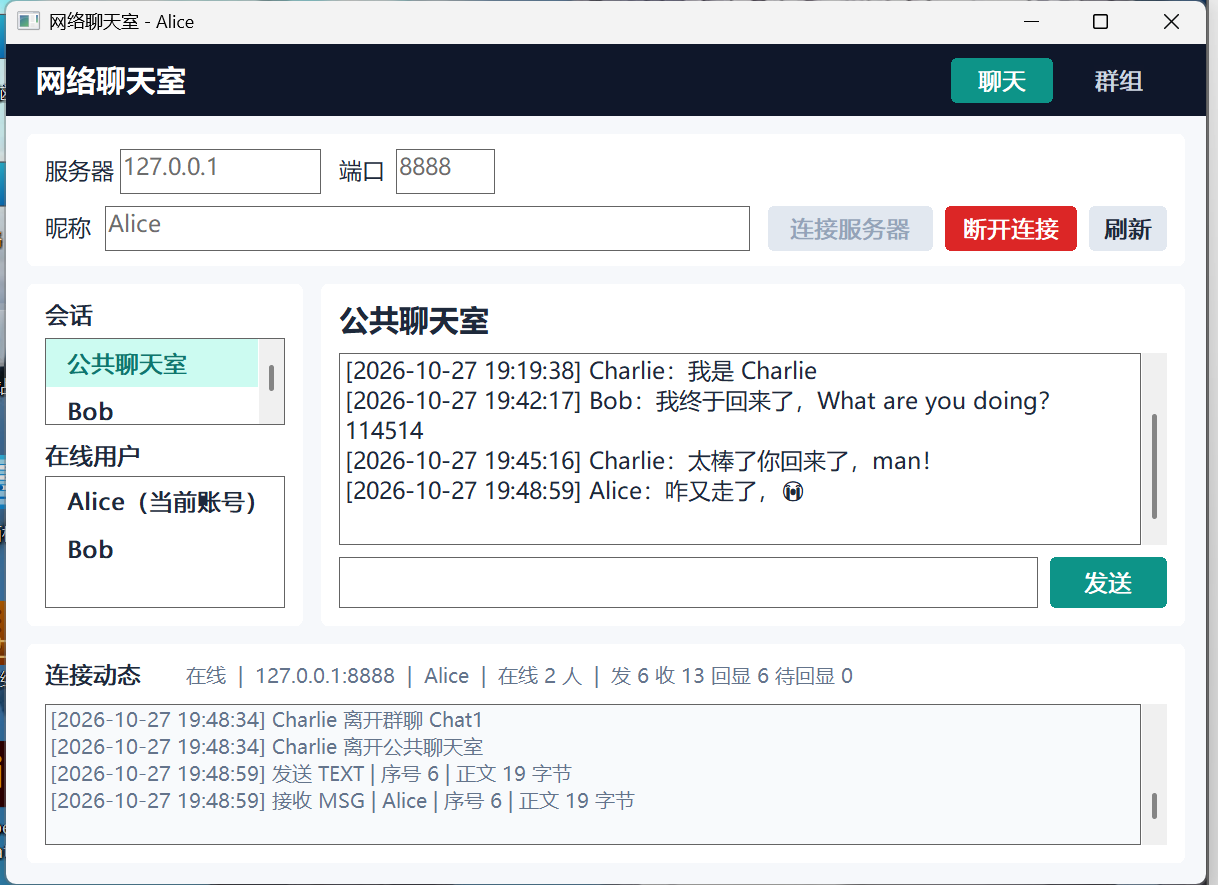
\includegraphics[width=\linewidth,height=10.0cm,keepaspectratio]{images/screen_55.png}
\captionof{figure}{Alice 继续发送公共消息}\label{fig:s55}
\par\smallskip{\raggedright\setlength{\parindent}{2em}\indent Alice 继续发送公共消息，聊天区出现新的本人回显。\par}
\end{minipage}\par\smallskip
\par\smallskip\noindent\begin{minipage}{\linewidth}\centering
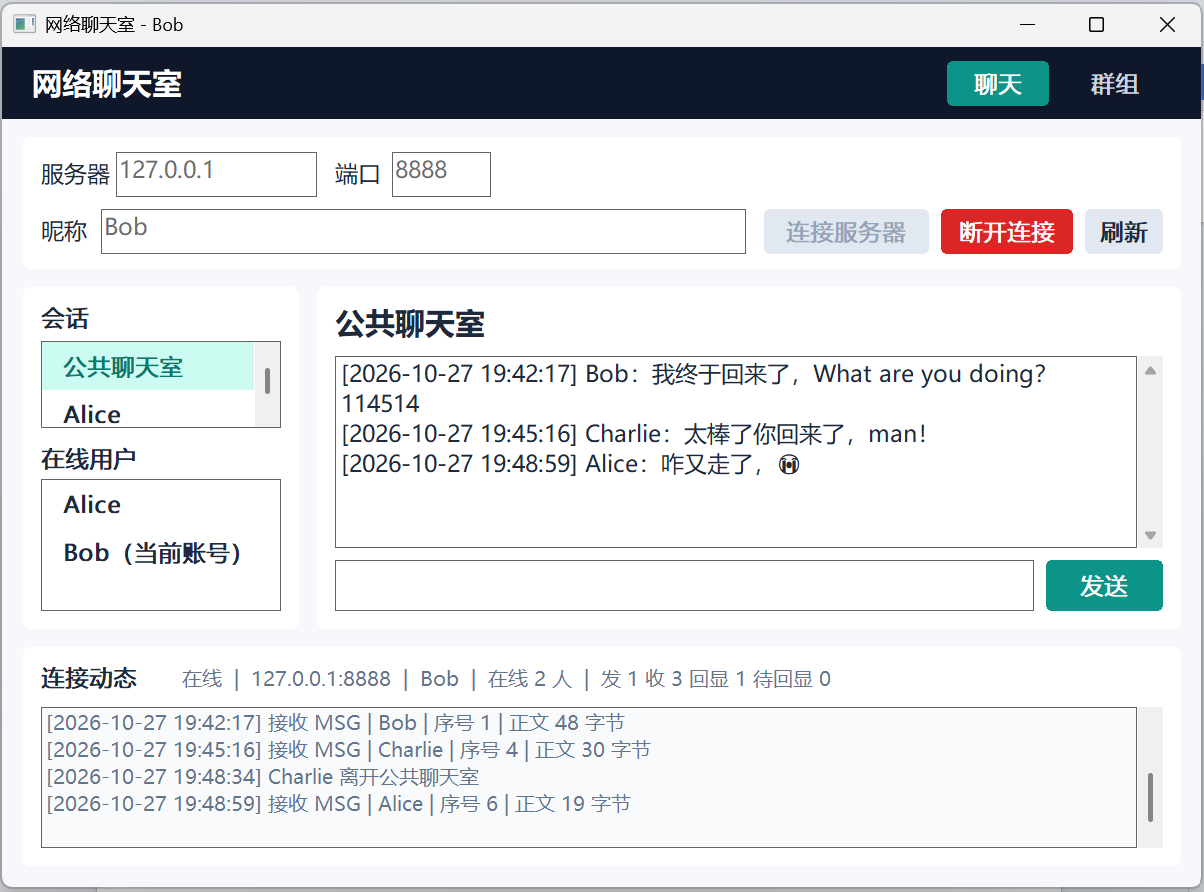
\includegraphics[width=\linewidth,height=10.0cm,keepaspectratio]{images/screen_56.png}
\captionof{figure}{Bob 继续接收公共消息}\label{fig:s56}
\par\smallskip{\raggedright\setlength{\parindent}{2em}\indent Bob 也收到这条发言，剩余两位用户可以继续聊天。\par}
\end{minipage}\par\smallskip
Charlie 退出后，其余两人的消息仍能互相送达，在线人数也维持为 2，表明关闭单个客户端只结束对应会话，其他连接继续运行。

\Needspace{10\baselineskip}
\section{自动化测试}
\subsection{测试方法}
界面演示呈现了会话和成员变化，边界输入及批量收发则由 C++ 测试程序重复执行。在 protocol\_tests.cpp 中直接调用协议函数，在 integration\_tests.cpp 中建立真实 TCP 连接，向 server.exe 提交请求并读取响应。

测试端以 Peer 保存套接字、半帧缓存及完整帧队列，读取时先取队列内容，再调用 recv，并通过 extract\_frames 恢复帧。每项断言输出 PASS 或 FAIL，最终汇总执行结果，接收辅助函数如下。

运行脚本后，依次完成编译、协议单元测试、独立服务器启动和网络测试，并保存日志。单元测试涵盖昵称、UTF-8、正文、数字范围及半帧提取，网络测试则给出经过实际连接后的响应。

\Needspace{4\baselineskip}
\VerbatimInput[fontsize=\small,breaklines=true,breakanywhere=true,numbers=left,firstnumber=1,numbersep=6pt,tabsize=4,baselinestretch=1.05]{code/listing_32.txt}
\medskip
\Needspace{4\baselineskip}
\VerbatimInput[fontsize=\small,breaklines=true,breakanywhere=true,numbers=left,firstnumber=1,numbersep=6pt,tabsize=4,baselinestretch=1.05]{code/listing_33.txt}
\medskip
\subsection{拆分发送}
拆分发送时，将带中文的 TEXT 按字节逐次提交，三个接收端最终都得到完整广播正文。因为网络栈仍可能合并相邻发送，单元测试中还直接分段输入字节，从而分别呈现缓存处理和真实网络收发的结果。

\Needspace{4\baselineskip}
\VerbatimInput[fontsize=\small,breaklines=true,breakanywhere=true,numbers=left,firstnumber=1,numbersep=6pt,tabsize=4,baselinestretch=1.05]{code/listing_34.txt}
\medskip
\subsection{合并发送}
合并发送时，将两条带 LF 的 TEXT 拼成一个字符串提交，接收后分别得到 first line、second line，序号为 1、2，说明同一批数据中的两帧已按结束符分开。

\Needspace{4\baselineskip}
\VerbatimInput[fontsize=\small,breaklines=true,breakanywhere=true,numbers=left,firstnumber=1,numbersep=6pt,tabsize=4,baselinestretch=1.05]{code/listing_35.txt}
\medskip
\subsection{边界输入}
边界测试分别发送重复昵称 Alice、非法昵称 bad-name、登录前 TEXT 和跳号序列，并继续提交合法请求。正文长度取 4096、4097 字节，分别得到正常转发和超长错误，边界值的处理结果随响应记录在日志中。

对应项目均输出 PASS，错误输入后的合法消息也继续得到正常响应，因此这组异常请求之后仍能在原连接上继续通信。

\subsection{并发交付}
并发测试中，LoadA、LoadB、LoadC 各提交 100 条消息，三个发送线程同时运行，每个接收端最终得到来自三位用户的 300 条广播。统计时按发送者和应用序号区分消息，处理过程如下。

\[
N_{\mathrm{message}}=3\times100=300
\]
\[
N_{\mathrm{delivery}}=300\times3=900
\]
对每个 MSG 读取发送者、序号、正文和时间格式，以集合统计唯一消息、重复项及缺失项。三个接收端均输出 received=300、missing=0、duplicate=0、invalid=0，合计记录 900 次应用消息交付。

\Needspace{4\baselineskip}
\VerbatimInput[fontsize=\small,breaklines=true,breakanywhere=true,numbers=left,firstnumber=1,numbersep=6pt,tabsize=4,baselinestretch=1.05]{code/listing_36.txt}
\medskip
\Needspace{4\baselineskip}
\VerbatimInput[fontsize=\small,breaklines=true,breakanywhere=true,numbers=left,firstnumber=1,numbersep=6pt,tabsize=4,baselinestretch=1.05]{code/listing_37.txt}
\medskip
\Needspace{4\baselineskip}
\VerbatimInput[fontsize=\small,breaklines=true,breakanywhere=true,numbers=left,firstnumber=1,numbersep=6pt,tabsize=4,baselinestretch=1.05]{code/listing_38.txt}
\medskip
\subsection{测试结果}
\begin{longtable}{@{}>{\raggedright\arraybackslash}p{0.113\linewidth}>{\raggedright\arraybackslash}p{0.685\linewidth}>{\raggedright\arraybackslash}p{0.141\linewidth}@{}}
\toprule
编号 & 测试项目 & 结果\\
\midrule\endfirsthead
\toprule
编号 & 测试项目 & 结果\\
\midrule\endhead
T01 & Alice 建连并完成 JOIN/WELCOME & PASS\\
T02 & Bob 同时在线 & PASS\\
T03 & Charlie 同时在线 & PASS\\
T04 & 重复昵称返回错误 & PASS\\
T05 & 非法昵称返回错误 & PASS\\
T06 & 登录前聊天返回错误 & PASS\\
T07 & 中英文、时间、竖线正文和三方广播 & PASS\\
T08 & 逐字节发送和 UTF-8 重组 & PASS\\
T09 & 一次发送两帧并分别提取 & PASS\\
T10 & 查询在线名单 & PASS\\
T11 & 错误序号返回错误 & PASS\\
T12 & 错误序号后恢复合法发送 & PASS\\
T13 & 完整交付 4096 字节正文 & PASS\\
T14 & 4097 字节正文返回超长错误 & PASS\\
T15 & QUIT 和 BYE 退出交互 & PASS\\
T16 & 建立三个并发负载会话 & PASS\\
T17 & 三位发送者各提交 100 条消息 & PASS\\
T18 & 三端共 900 次应用消息交付 & PASS\\
T19 & 建立私聊和群聊测试会话 & PASS\\
T20 & 私聊发送方和目标接收 & PASS\\
T21 & 建群、加入、添加成员和群列表 & PASS\\
T22 & 群内消息转发 & PASS\\
T23 & 被添加成员收到群消息 & PASS\\
T24 & 退群、离线私聊目标和群成员校验 & PASS\\*
\bottomrule
\caption{网络测试记录}\\
\end{longtable}
网络测试最终输出 TOTAL PASS=24 FAIL=0，各项结果见表。随后另行进行图形界面抓包演示，记录手动操作产生的握手、聊天传输和连接释放。

\Needspace{4\baselineskip}
\VerbatimInput[fontsize=\small,breaklines=true,breakanywhere=true,numbers=left,firstnumber=1,numbersep=6pt,tabsize=4,baselinestretch=1.05]{code/listing_39.txt}
\medskip
\Needspace{10\baselineskip}
\section{TCP 抓包}
\subsection{启动捕获}
重新进行带抓包的演示时，在 Wireshark 中选择回环捕获接口，设置捕获过滤器 tcp port 8888，开始捕获后再连接三位用户；显示过滤器使用 tcp.port == 8888，列表中仅呈现实验端口流量。

捕获过滤器决定写入文件的流量范围，显示过滤器只影响列表呈现。由空列表开始，依次进行登录、公聊、私聊、群操作、断开和重连，操作产生的分组随时间增加。

\par\smallskip\noindent\begin{minipage}{\linewidth}\centering
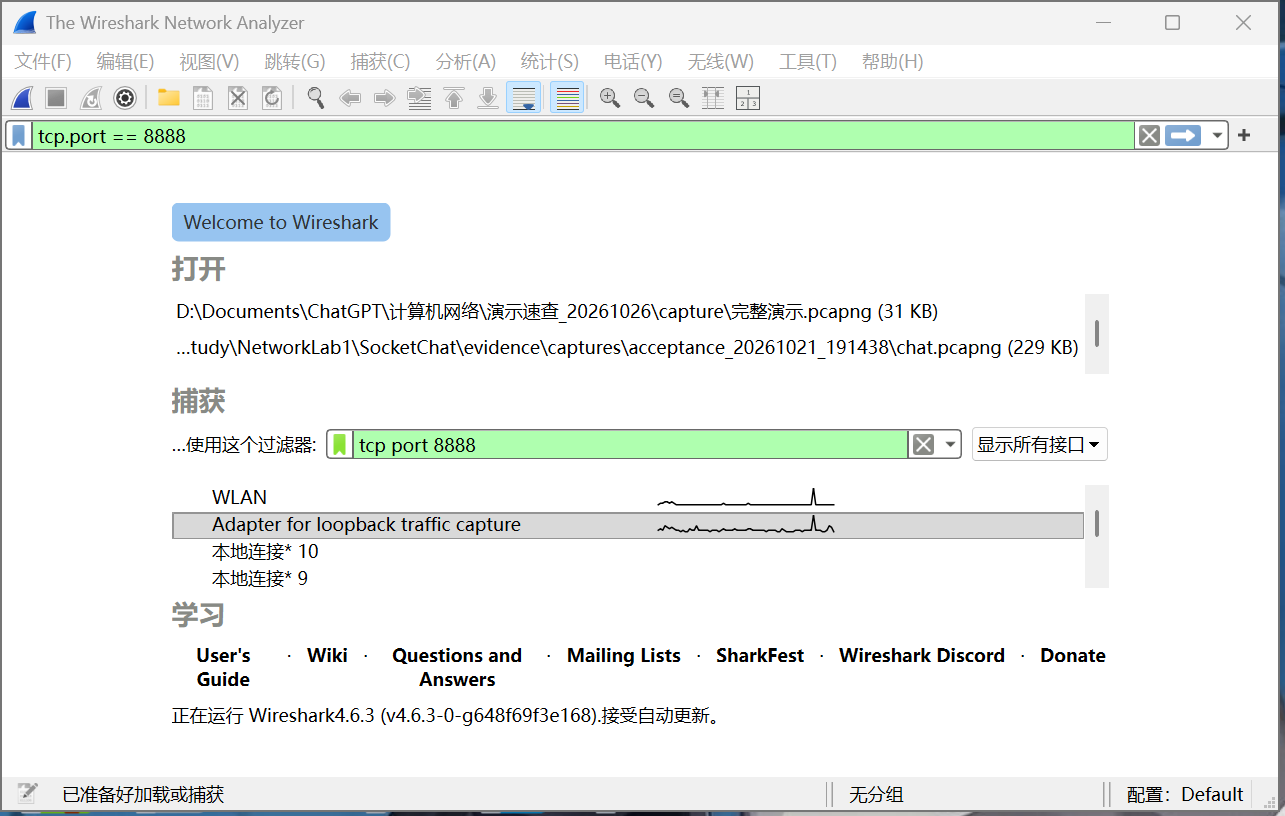
\includegraphics[width=\linewidth,height=10.0cm,keepaspectratio]{images/screen_57.png}
\captionof{figure}{回环捕获接口及过滤器}\label{fig:s57}
\par\smallskip{\raggedright\setlength{\parindent}{2em}\indent 捕获前选择回环接口，捕获过滤器填为 tcp port 8888，记录范围限定为实验端口。\par}
\end{minipage}\par\smallskip
\par\smallskip\noindent\begin{minipage}{\linewidth}\centering
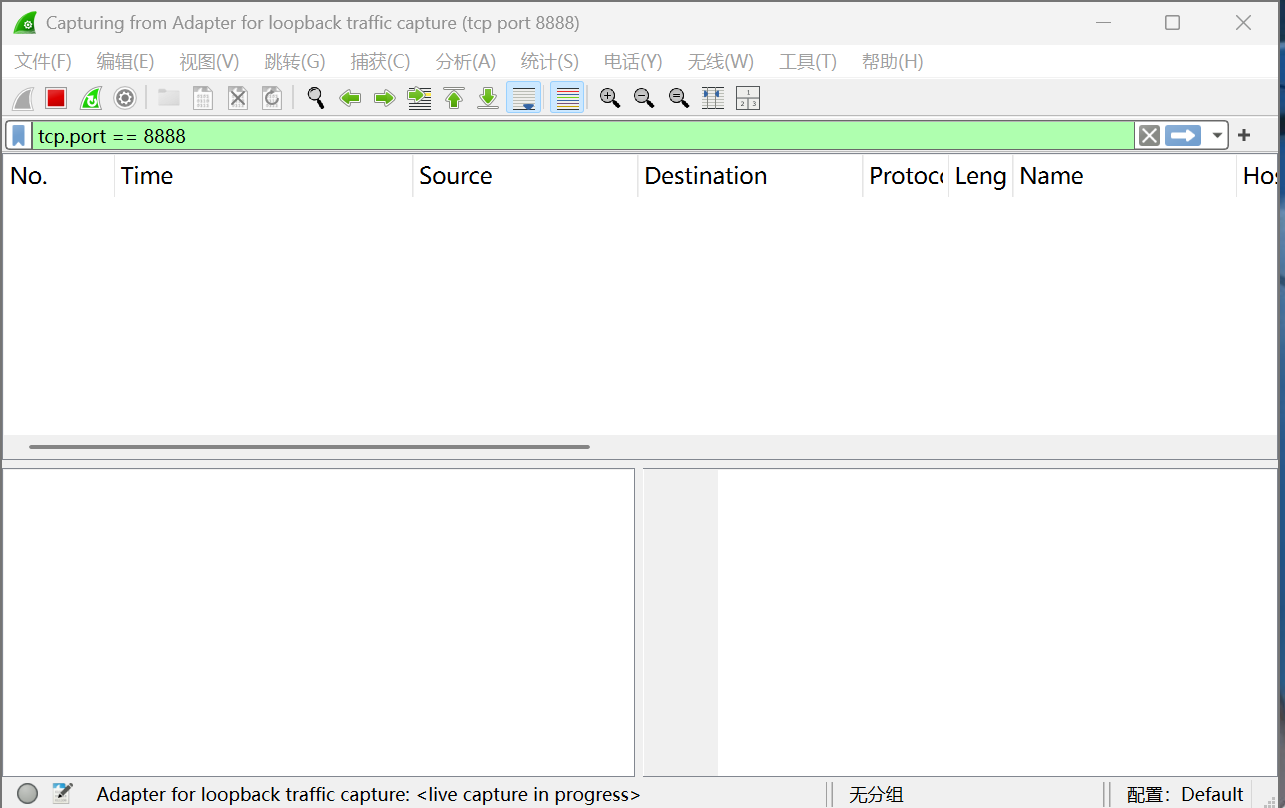
\includegraphics[width=\linewidth,height=10.0cm,keepaspectratio]{images/screen_58.png}
\captionof{figure}{捕获开始时的空列表}\label{fig:s58}
\par\smallskip{\raggedright\setlength{\parindent}{2em}\indent 开始捕获后使用 tcp.port == 8888 显示过滤器，此时列表仍为空，客户端尚未开始这一轮连接。\par}
\end{minipage}\par\smallskip
\subsection{三人登录}
Alice、Bob、Charlie 依次登录后，各客户端显示人数和名单变化，Wireshark 同时出现相应 TCP 分组，下面按操作顺序放置客户端页面和流量页面。

\par\smallskip\noindent\begin{minipage}{\linewidth}\centering
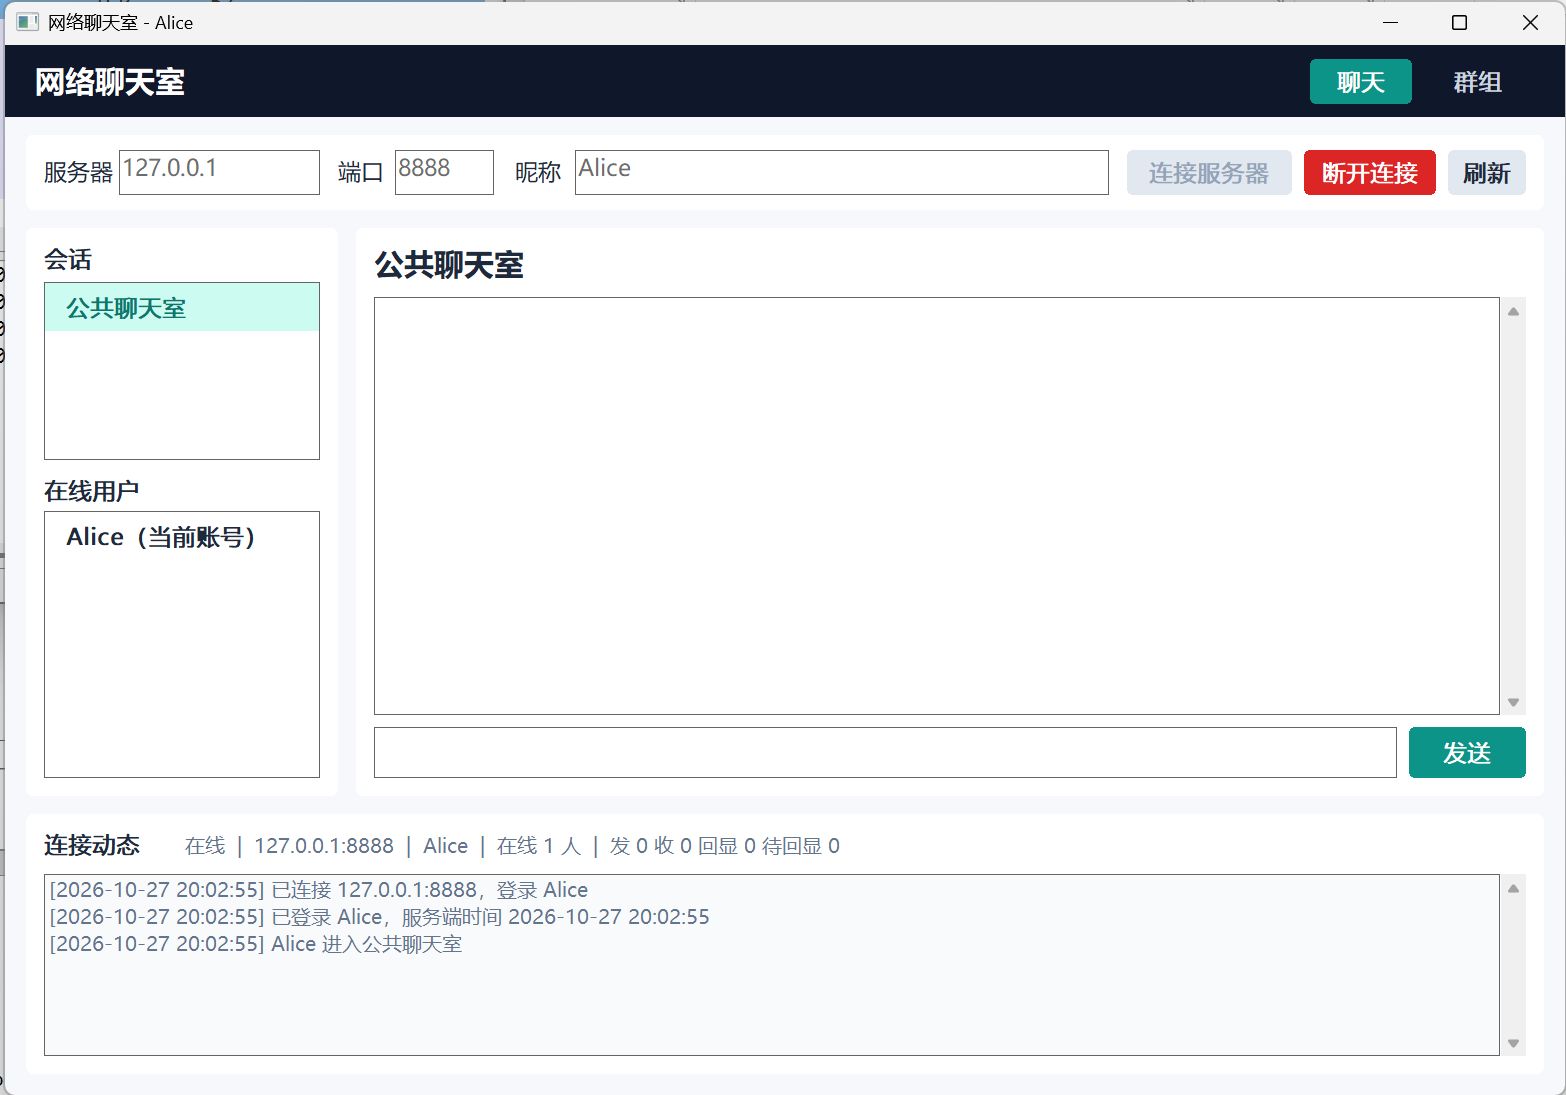
\includegraphics[width=\linewidth,height=10.0cm,keepaspectratio]{images/screen_59.png}
\captionof{figure}{抓包期间 Alice 登录}\label{fig:s59}
\par\smallskip{\raggedright\setlength{\parindent}{2em}\indent Alice 首先登录，窗口中显示登录成功，在线人数为 1。\par}
\end{minipage}\par\smallskip
\par\smallskip\noindent\begin{minipage}{\linewidth}\centering
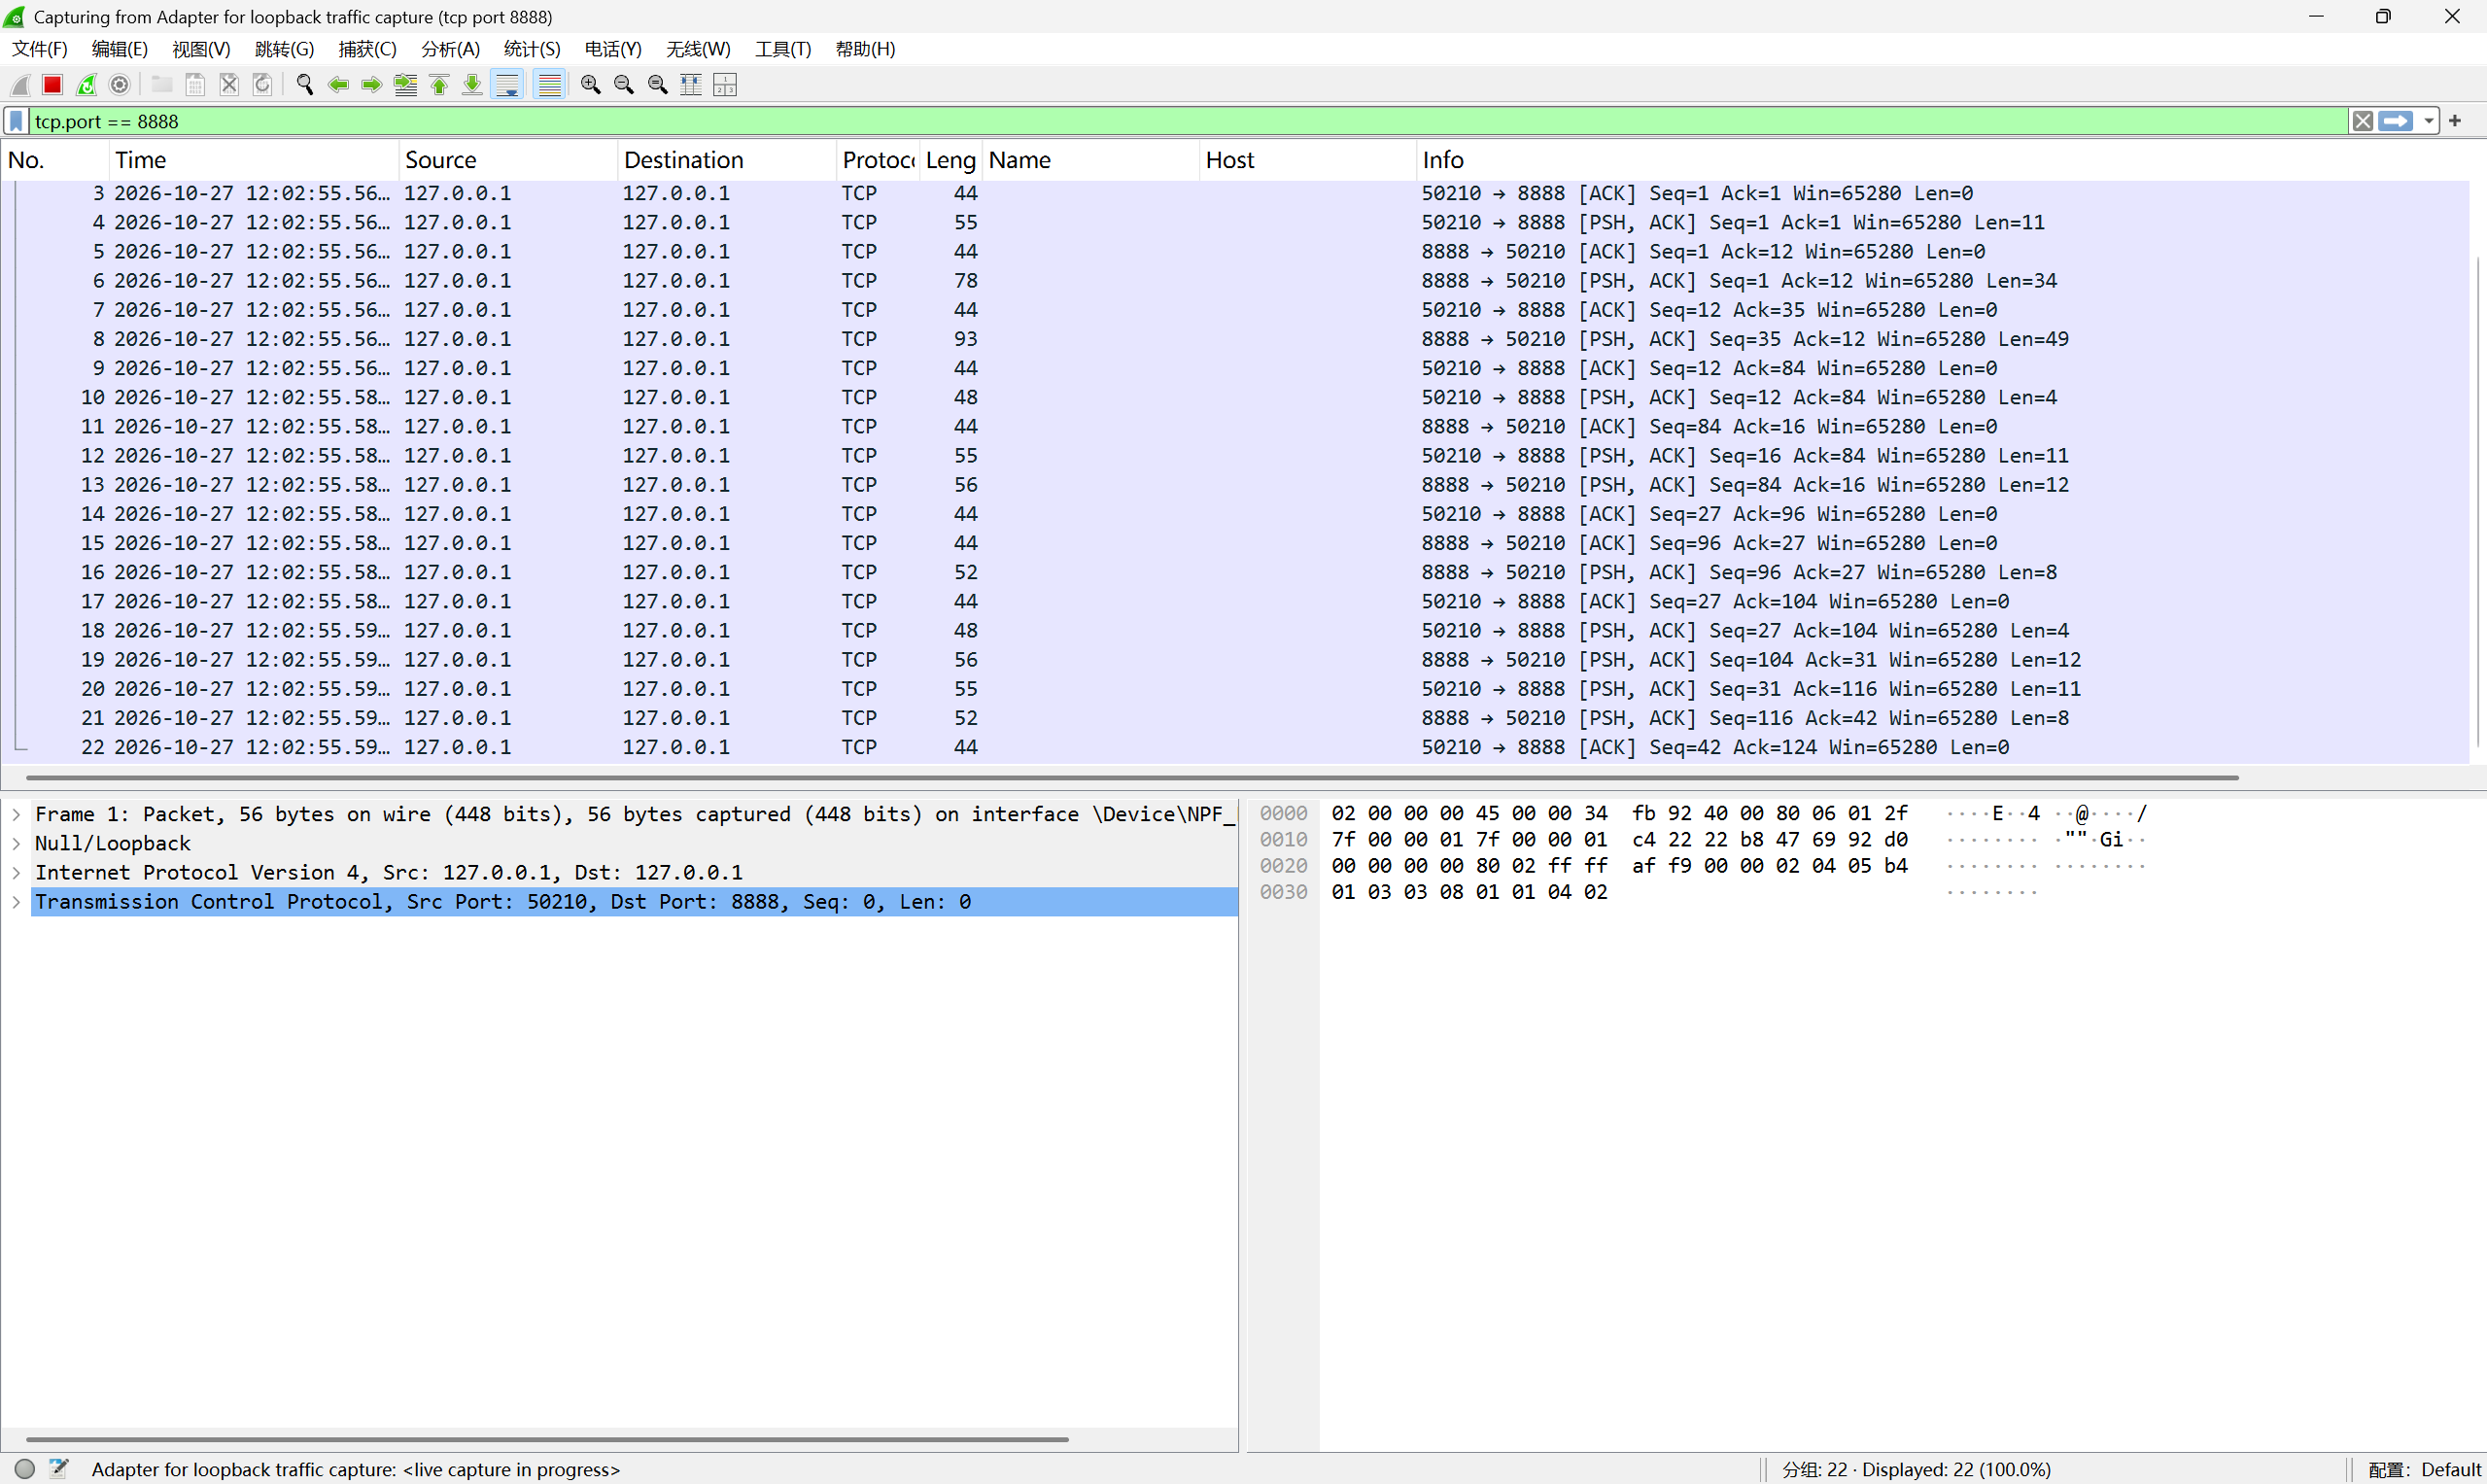
\includegraphics[width=\linewidth,height=10.0cm,keepaspectratio]{images/screen_60.png}
\captionof{figure}{Alice 登录产生的 TCP 流量}\label{fig:s60}
\par\smallskip{\raggedright\setlength{\parindent}{2em}\indent Wireshark 随后出现建连及登录阶段的 TCP 分组，具体帧号在握手分析中列出。\par}
\end{minipage}\par\smallskip
\par\smallskip\noindent\begin{minipage}{\linewidth}\centering
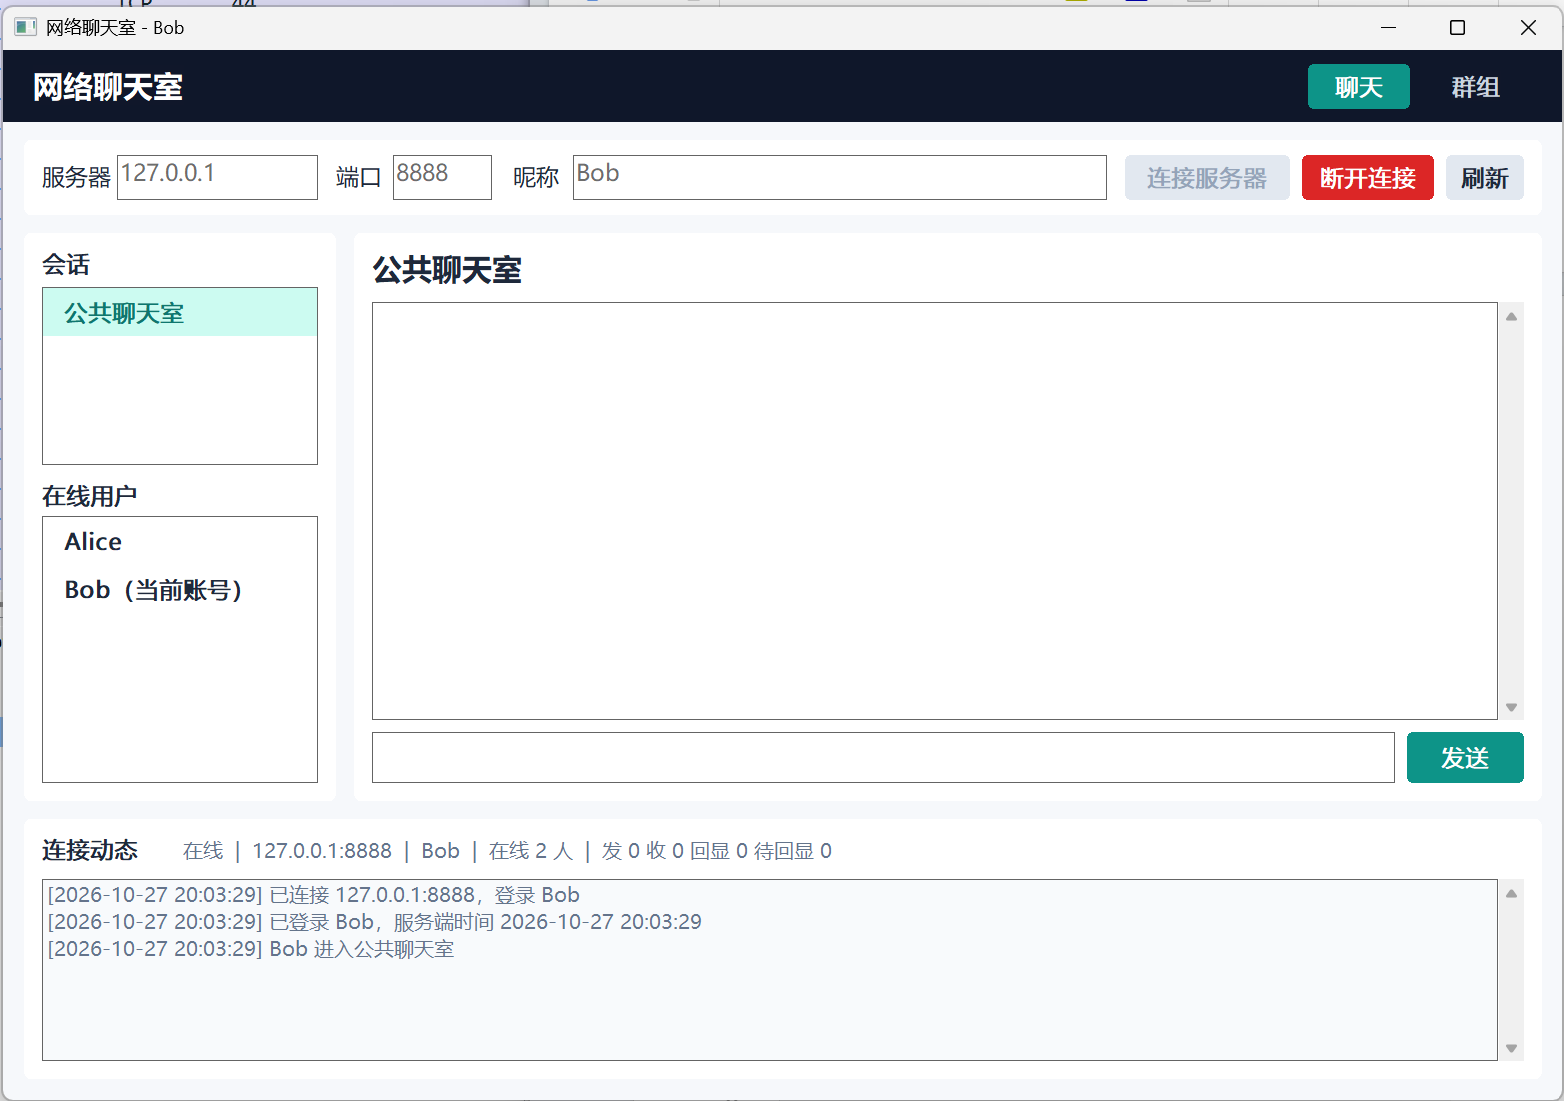
\includegraphics[width=\linewidth,height=10.0cm,keepaspectratio]{images/screen_61.png}
\captionof{figure}{抓包期间 Bob 登录}\label{fig:s61}
\par\smallskip{\raggedright\setlength{\parindent}{2em}\indent Bob 登录后，在线人数变为 2，名单增加第二位用户。\par}
\end{minipage}\par\smallskip
\par\smallskip\noindent\begin{minipage}{\linewidth}\centering
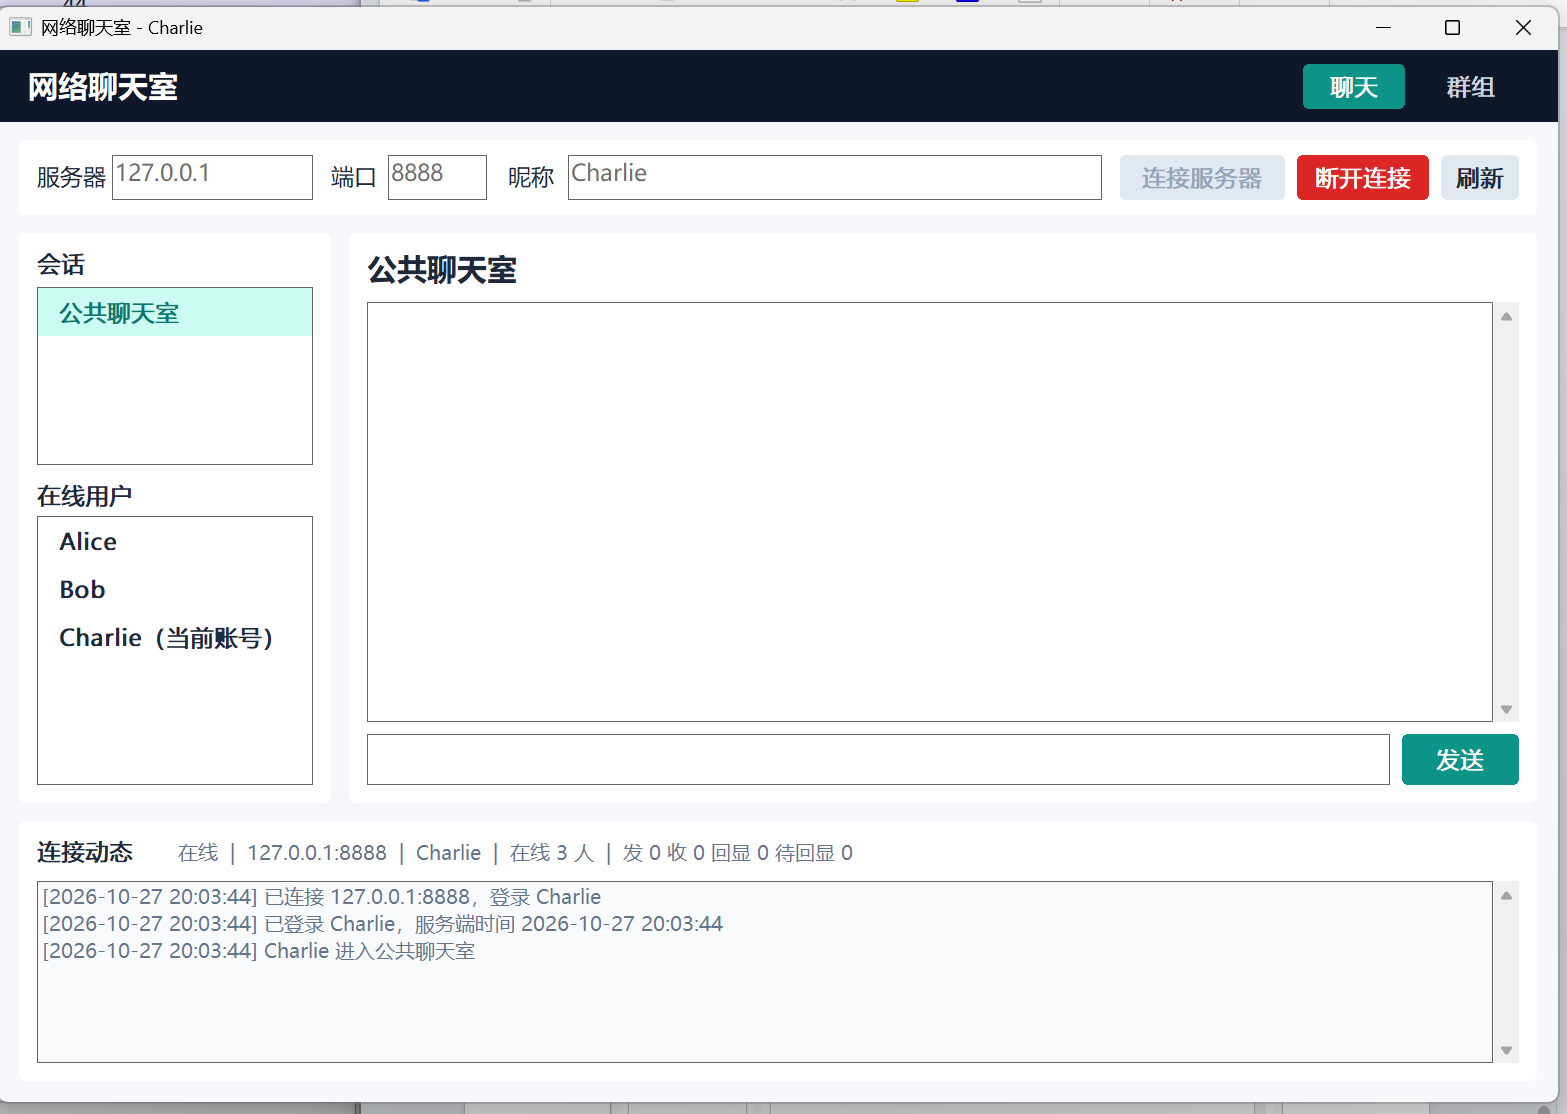
\includegraphics[width=\linewidth,height=10.0cm,keepaspectratio]{images/screen_62.png}
\captionof{figure}{抓包期间 Charlie 登录}\label{fig:s62}
\par\smallskip{\raggedright\setlength{\parindent}{2em}\indent Charlie 随后登录，在线名单恢复三位用户。\par}
\end{minipage}\par\smallskip
\par\smallskip\noindent\begin{minipage}{\linewidth}\centering
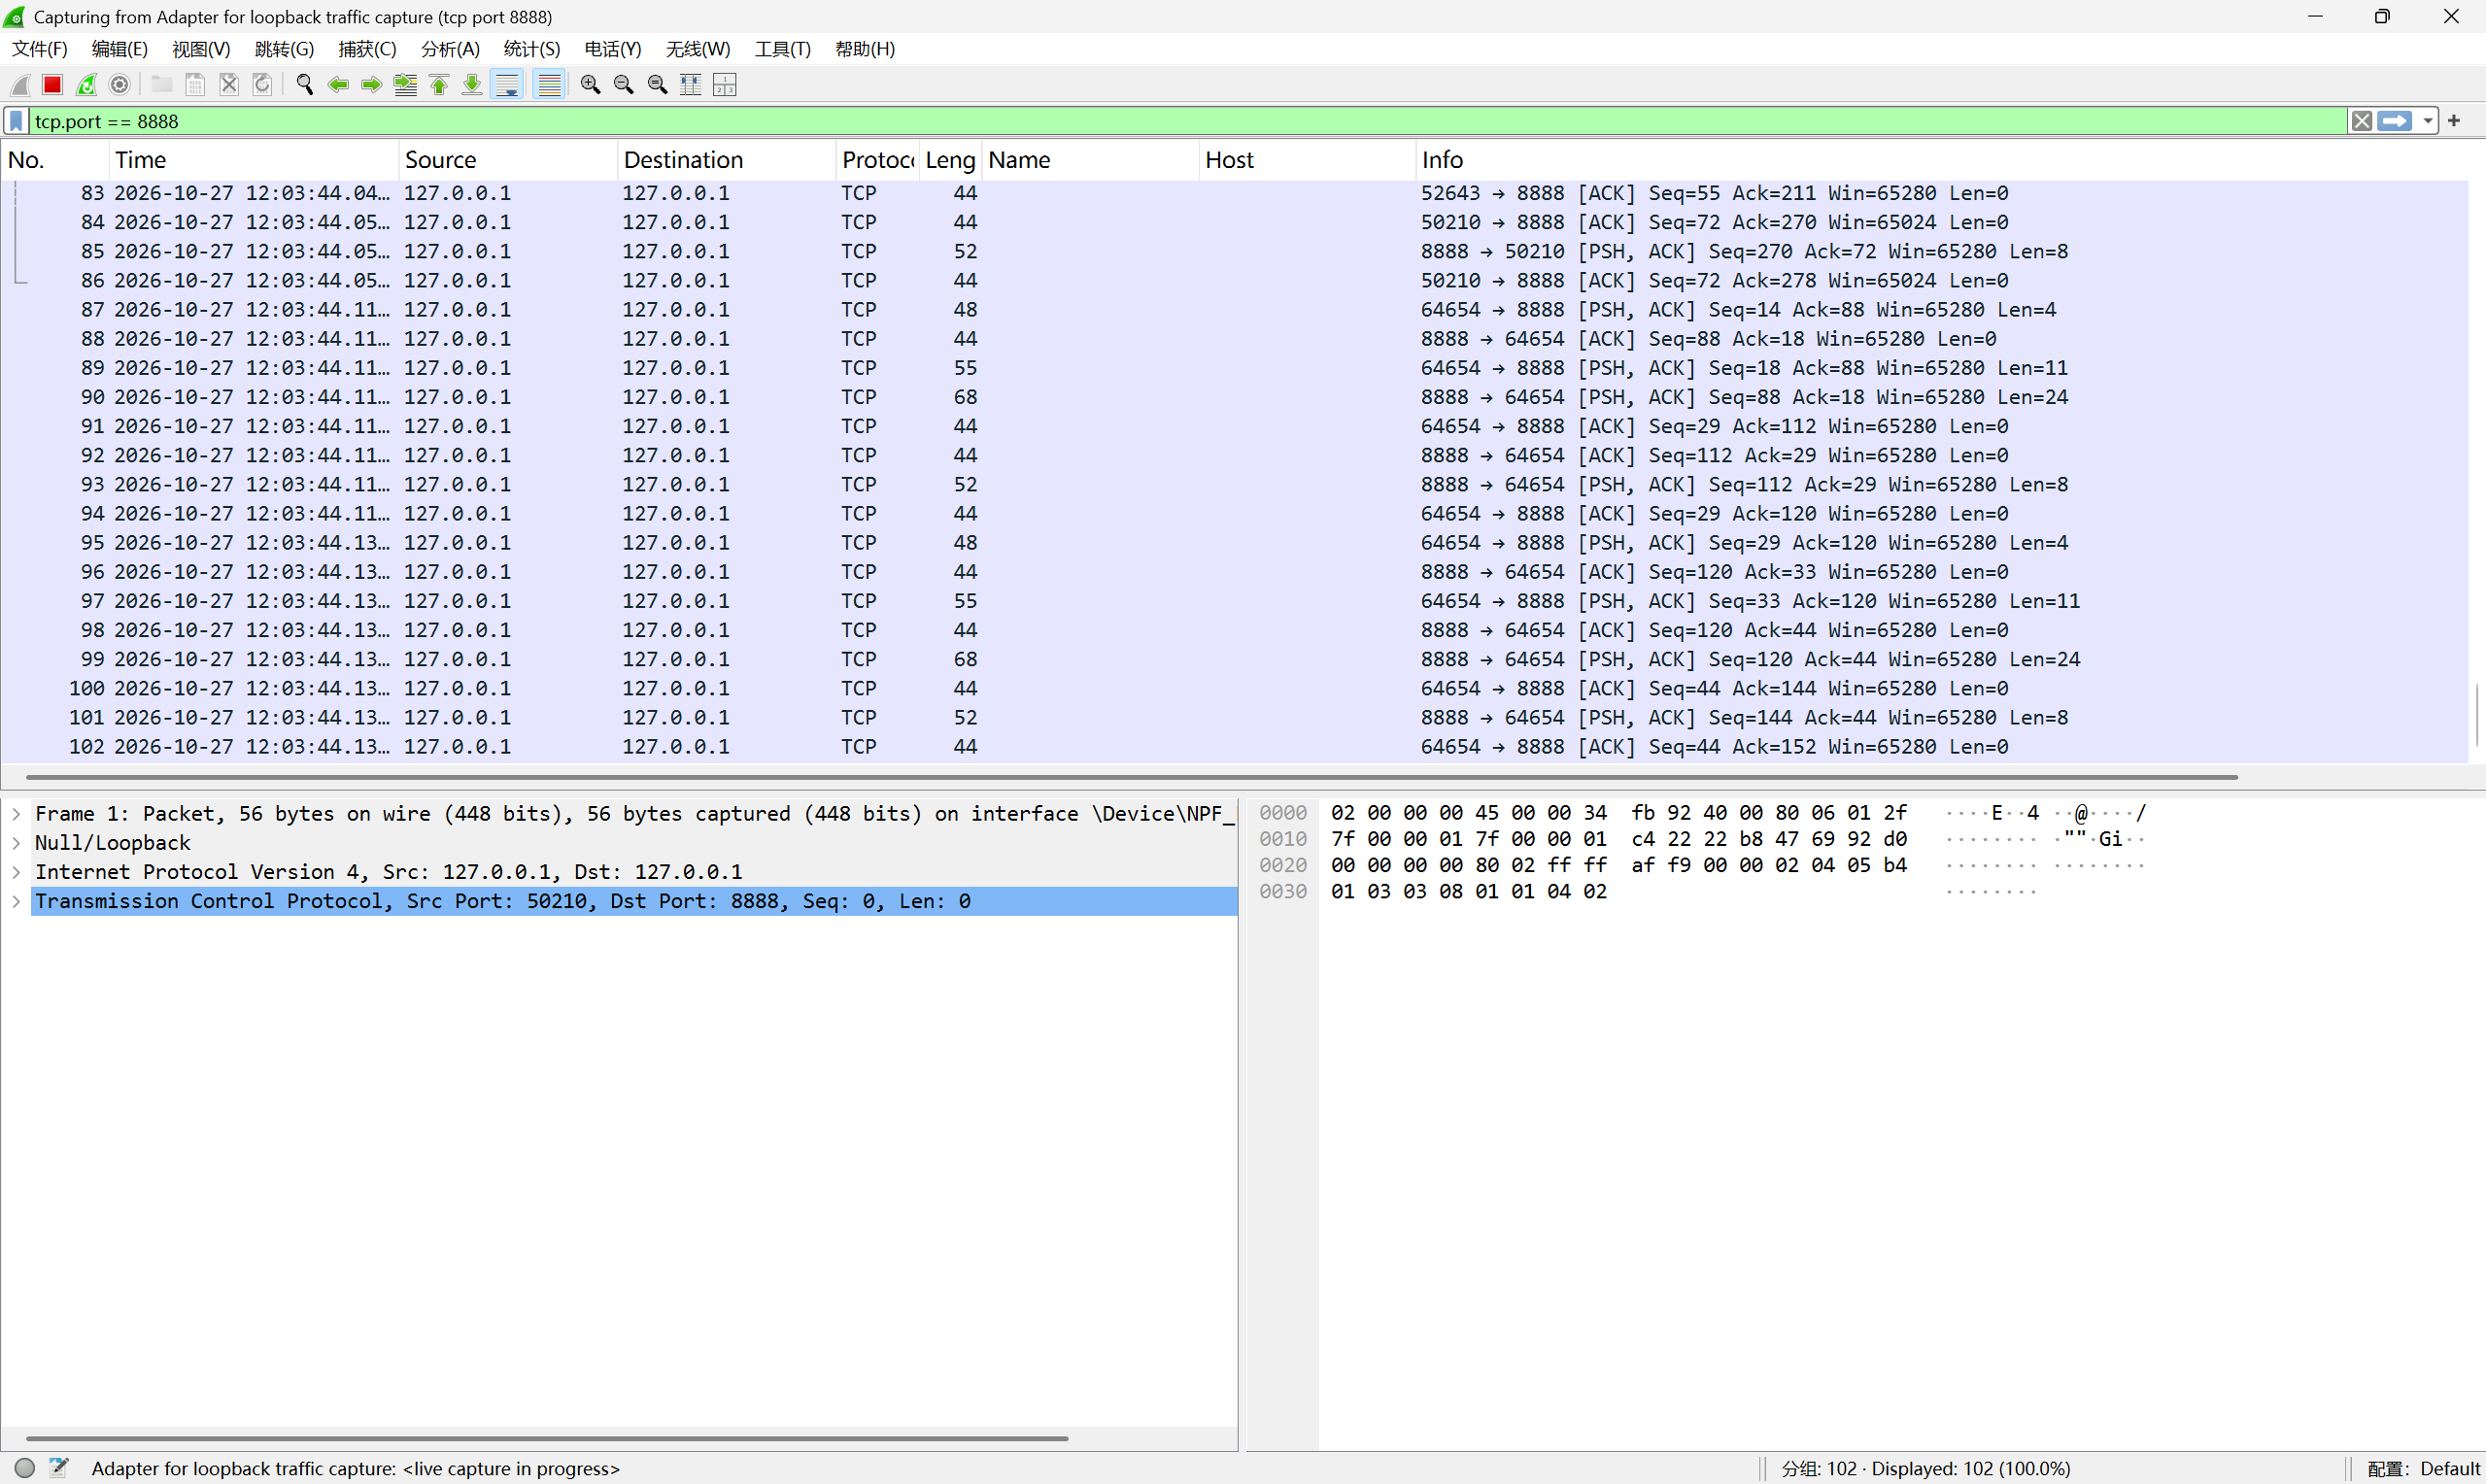
\includegraphics[width=\linewidth,height=10.0cm,keepaspectratio]{images/screen_63.png}
\captionof{figure}{三人登录后的 TCP 流量}\label{fig:s63}
\par\smallskip{\raggedright\setlength{\parindent}{2em}\indent 流量列表中已经包含三条连接，通过各客户端临时端口可以区分对应的 TCP 流。\par}
\end{minipage}\par\smallskip
在完整抓包中，首次连接的临时端口分别为 Alice 的 50210、Bob 的 52643、Charlie 的 64654，对应 tcp.stream 0、1、2，目的端口均为服务器的 8888。

\par\medskip\noindent\begin{minipage}{\linewidth}\centering
\begin{tabular}{@{}>{\raggedright\arraybackslash}p{0.310\linewidth}>{\raggedright\arraybackslash}p{0.164\linewidth}>{\raggedright\arraybackslash}p{0.219\linewidth}>{\raggedright\arraybackslash}p{0.219\linewidth}@{}}
\toprule
用户 & 流编号 & 客户端端口 & JOIN 帧号\\
\midrule
Alice & 0 & 50210 & 4\\
Bob & 1 & 52643 & 26\\
Charlie 首次连接 & 2 & 64654 & 61\\
Charlie 重新连接 & 3 & 59815 & 299\\
\bottomrule
\end{tabular}
\captionof{table}{抓包中的连接}
\end{minipage}\par\medskip
\subsection{公共消息流量}
Alice 输入“抓公共消息，大家好，Hello TCP!”后，聊天区出现本人回显，抓包列表随之增加数据和 ACK。完整文件第 103 帧包含 TEXT|\allowbreak{}1，之后可在三条在线连接中找到 MSG 转发。

\par\smallskip\noindent\begin{minipage}{\linewidth}\centering
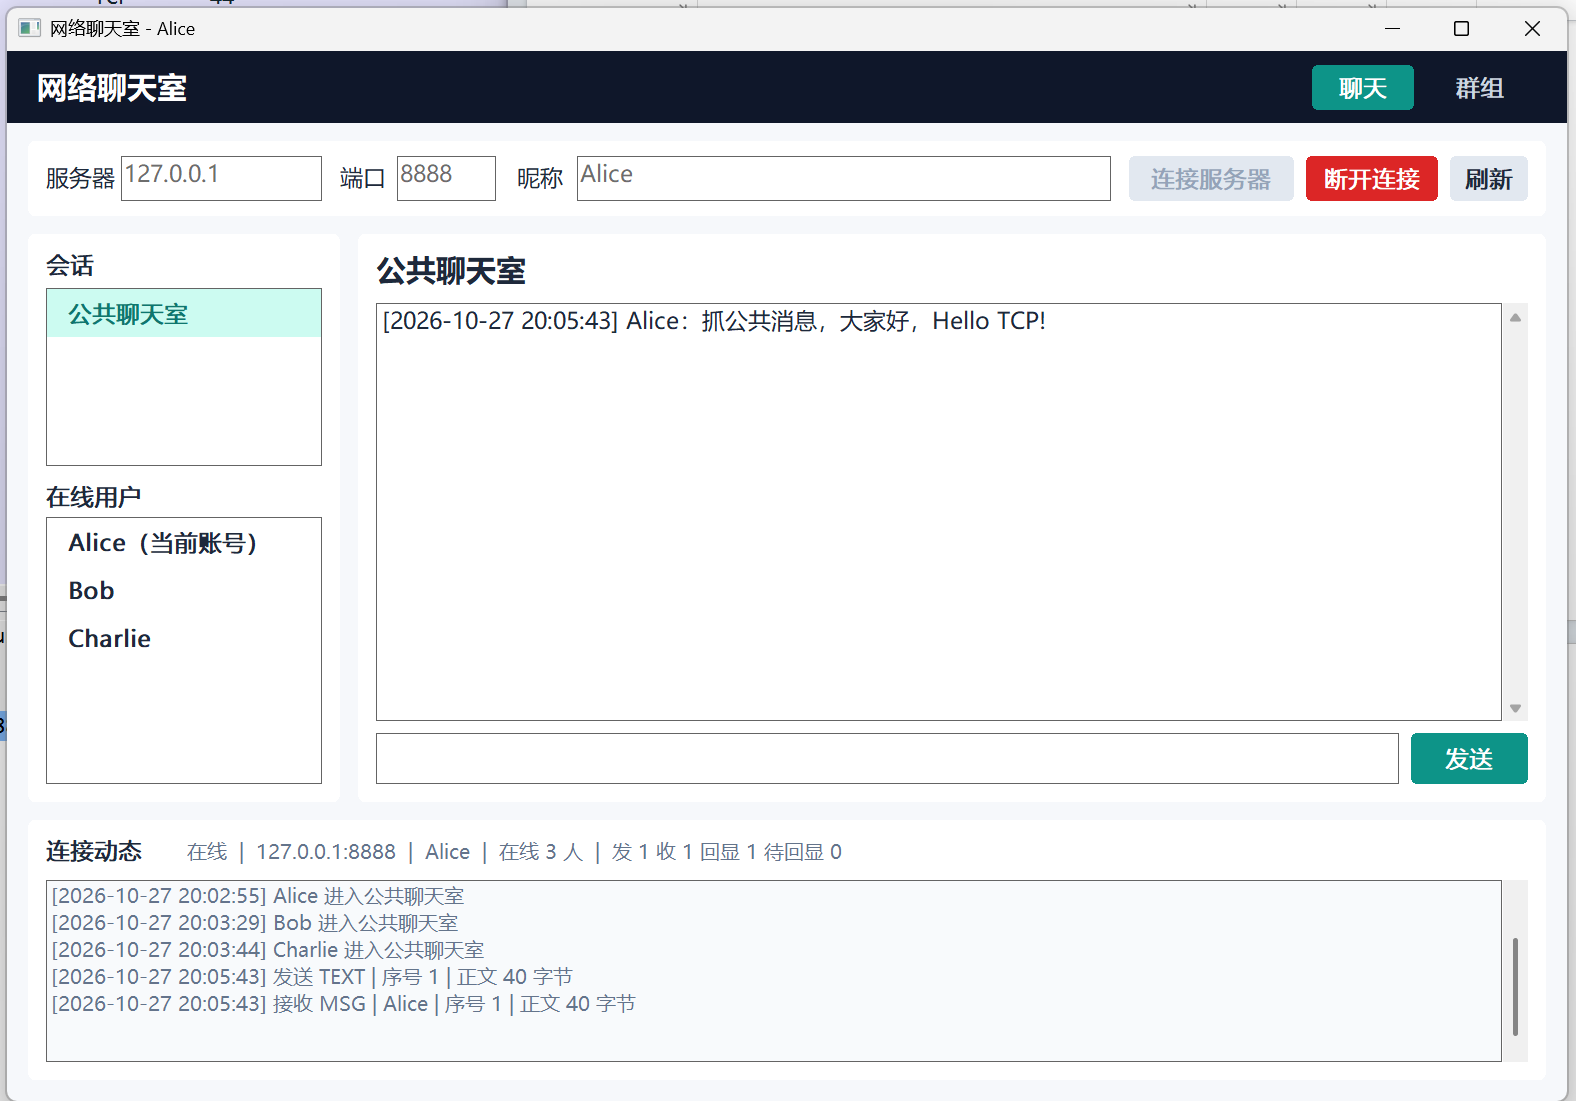
\includegraphics[width=\linewidth,height=10.0cm,keepaspectratio]{images/screen_64.png}
\captionof{figure}{用于抓包的公共发言}\label{fig:s64}
\par\smallskip{\raggedright\setlength{\parindent}{2em}\indent Alice 输入“抓公共消息，大家好，Hello TCP!”后，公共会话出现这条中英文发言和本人回显。\par}
\end{minipage}\par\smallskip
\par\smallskip\noindent\begin{minipage}{\linewidth}\centering
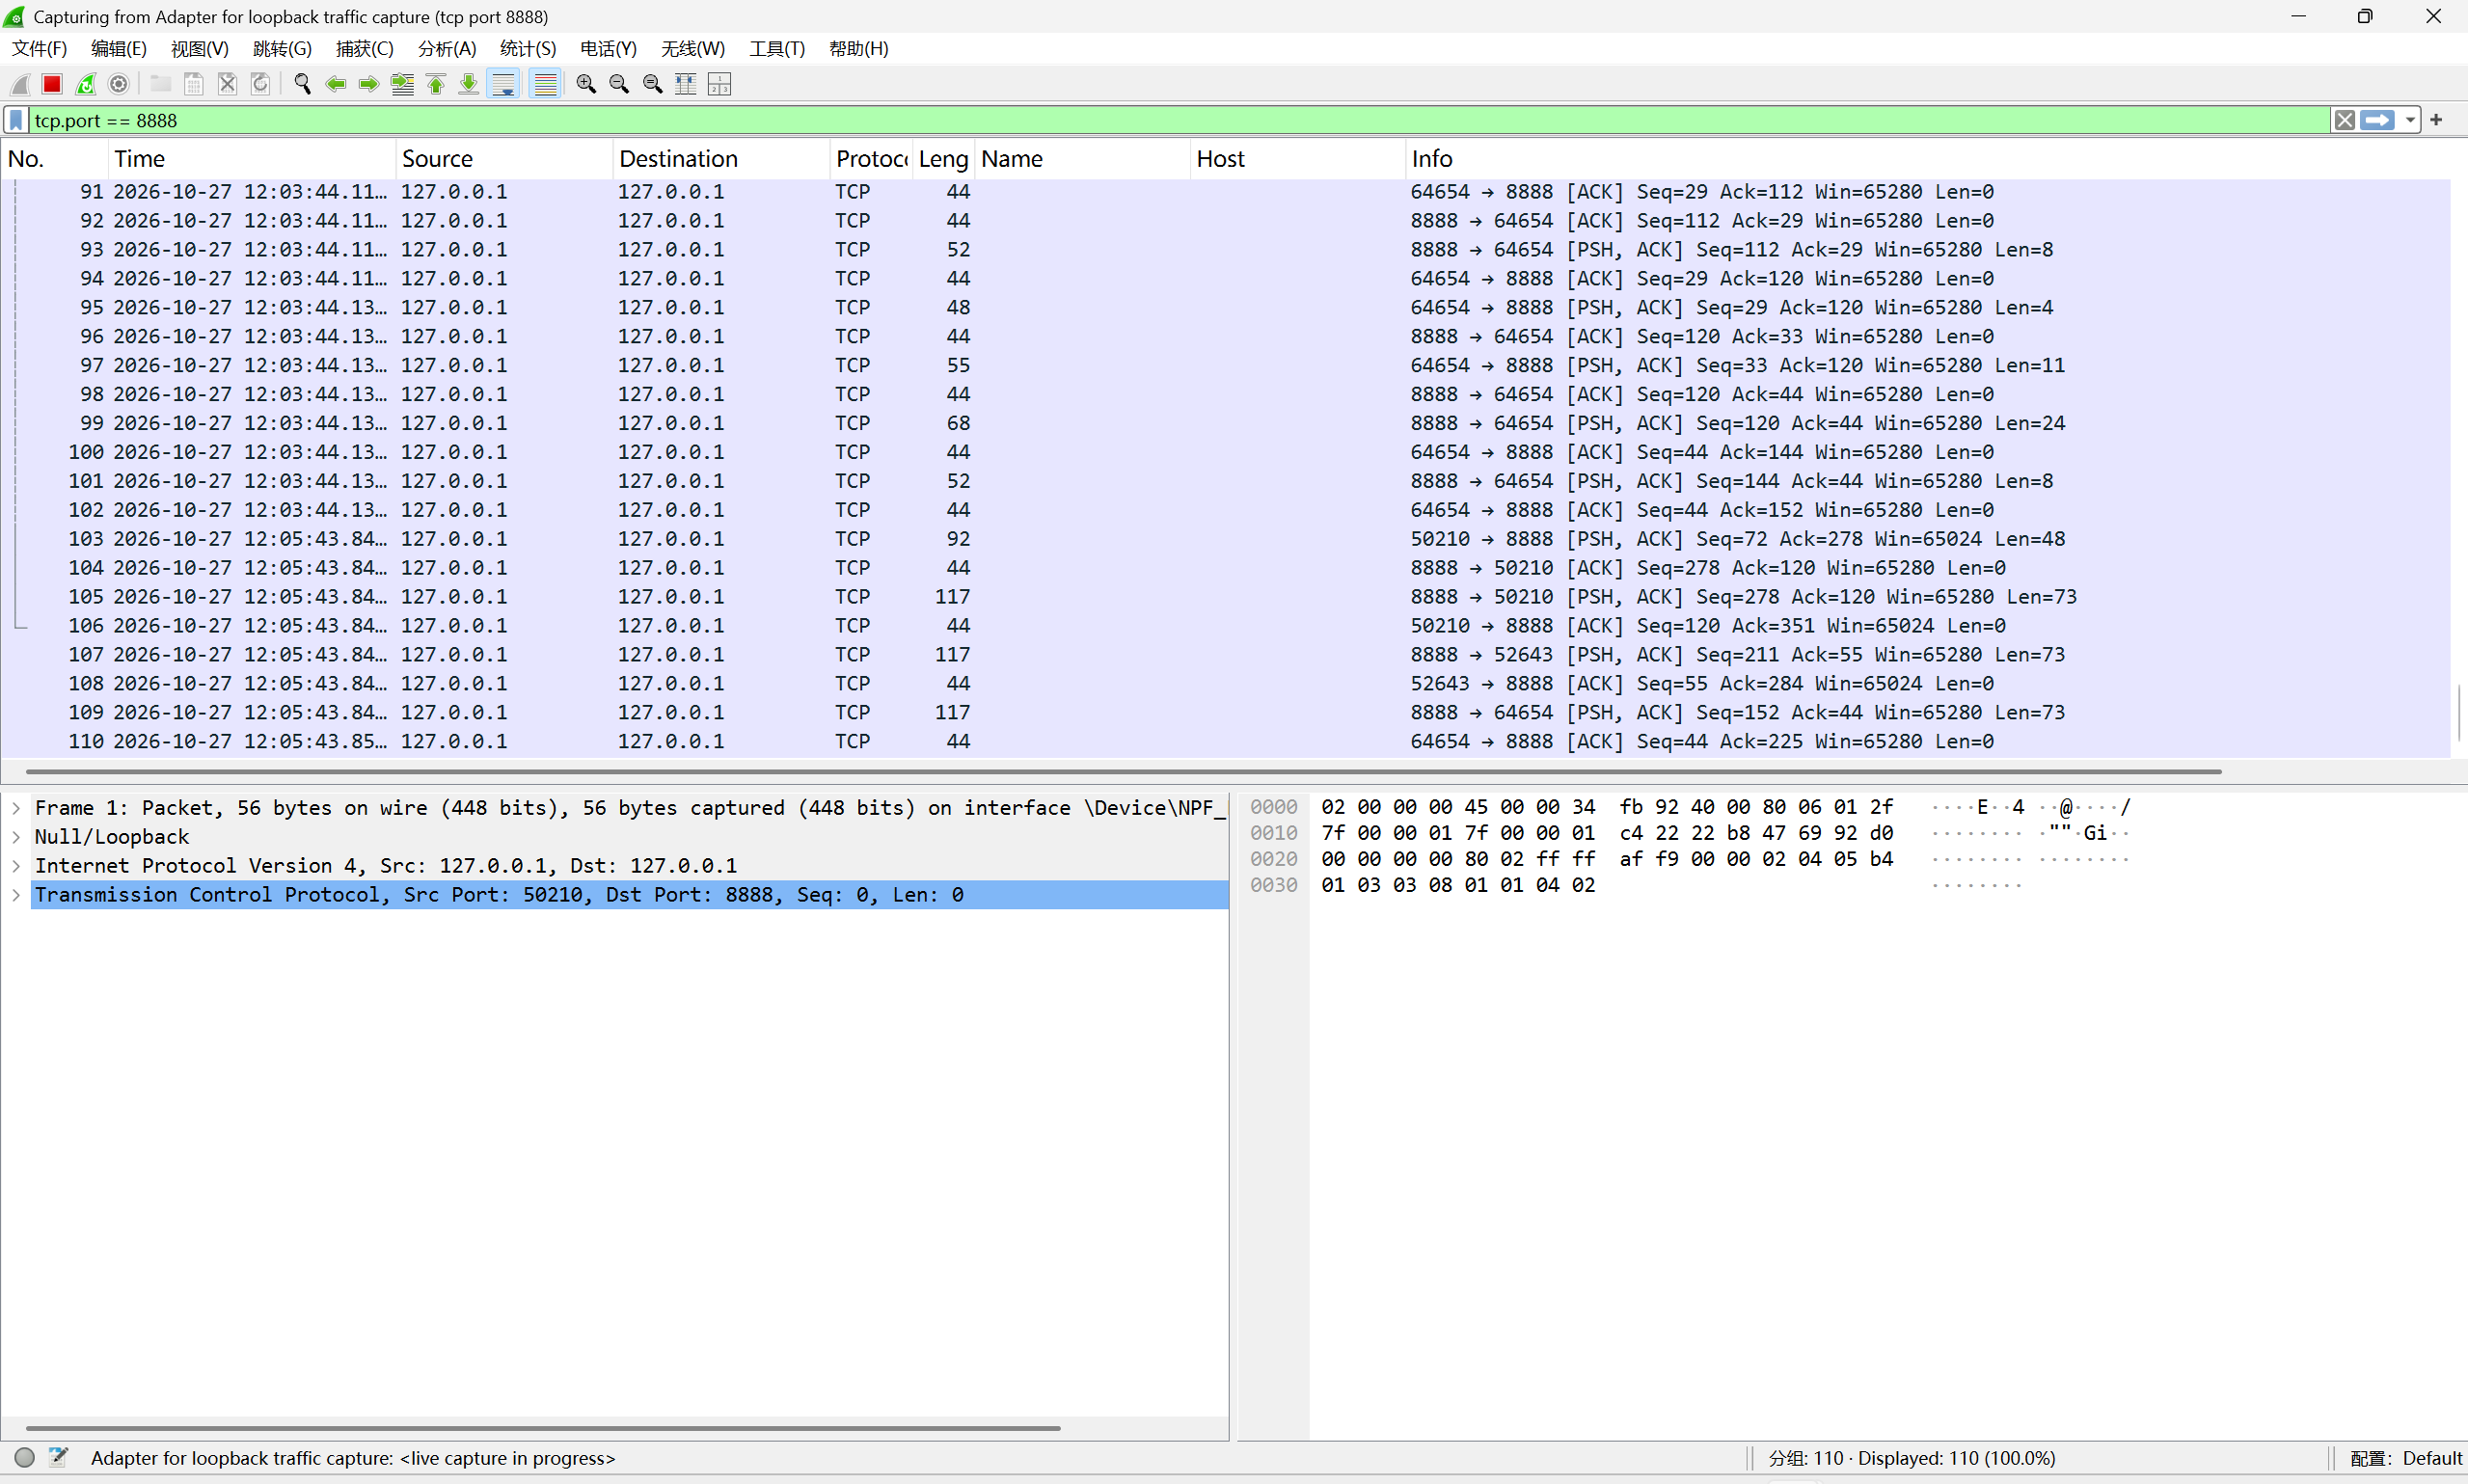
\includegraphics[width=\linewidth,height=10.0cm,keepaspectratio]{images/screen_65.png}
\captionof{figure}{公共发言对应的 TCP 流量}\label{fig:s65}
\par\smallskip{\raggedright\setlength{\parindent}{2em}\indent 列表新增客户端数据、服务器转发和 ACK，重组负载后可读到相应 TEXT、MSG。\par}
\end{minipage}\par\smallskip
\subsection{私聊流量}
在 Alice 中向 Bob 发送“抓私聊，Hi，Bob”，第 111 帧记录 PM|\allowbreak{}2|\allowbreak{}Bob，随后向 Alice 回显、向 Bob 转发。列表中可见数据及 ACK，重组相应 TCP 流后能够读到完整正文。

\par\smallskip\noindent\begin{minipage}{\linewidth}\centering
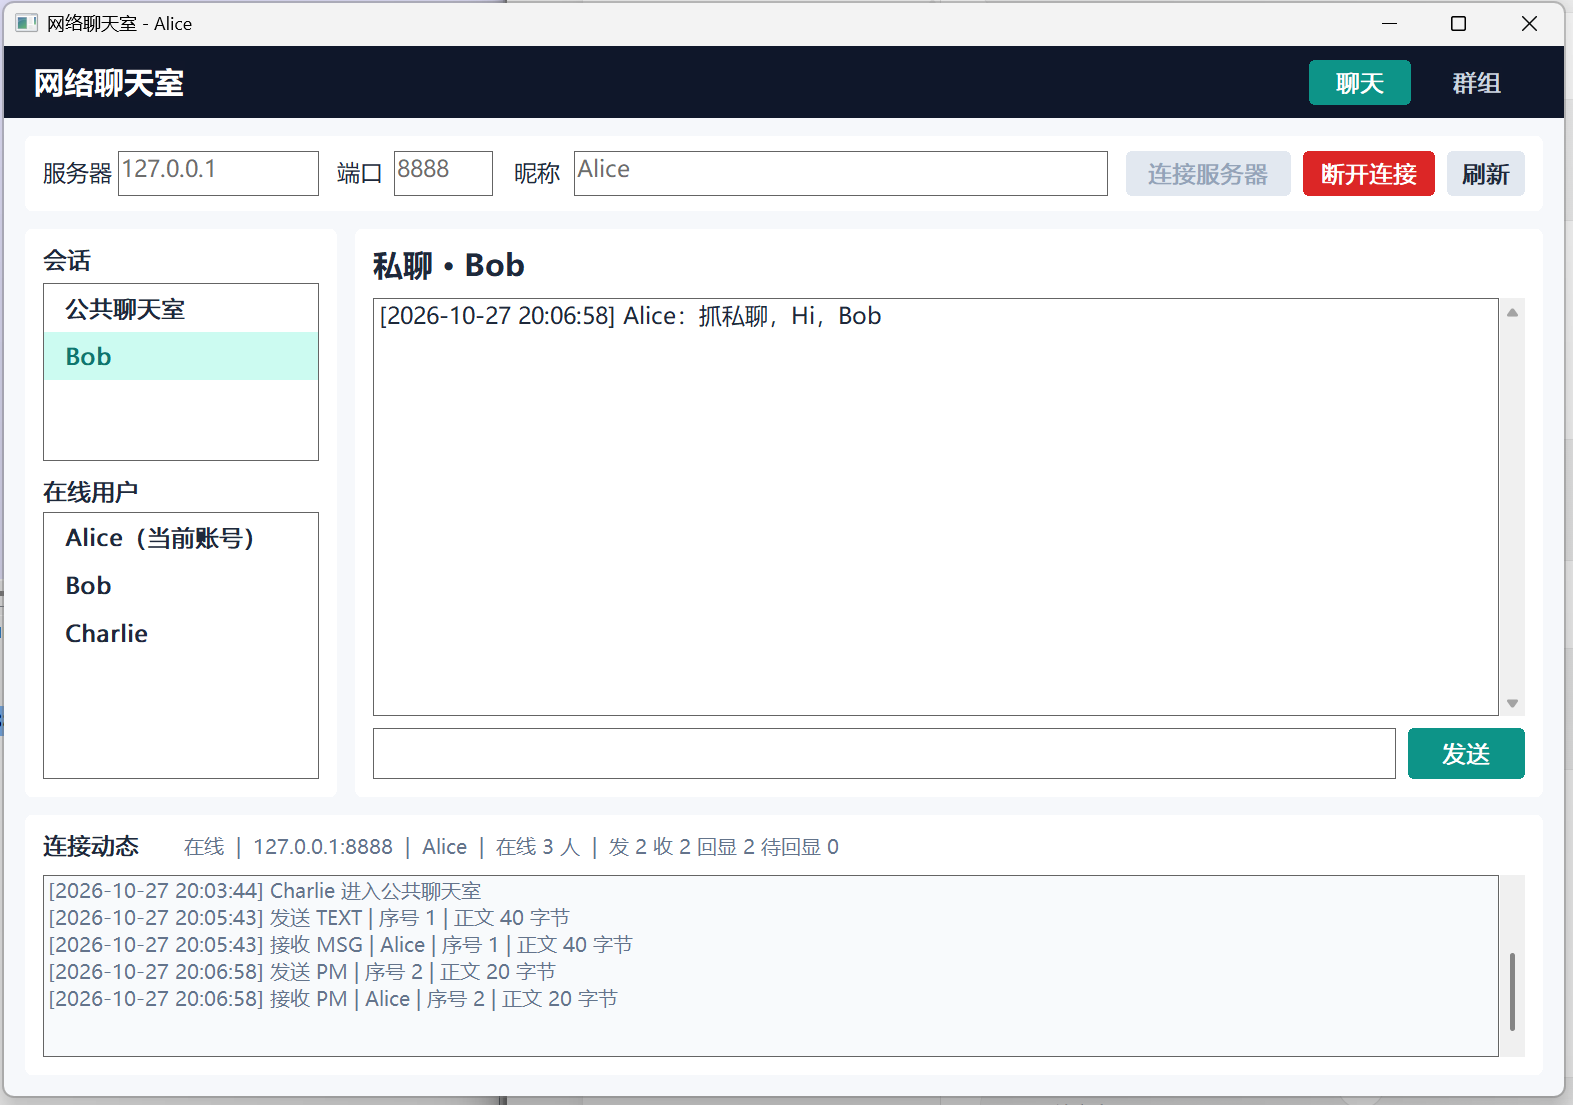
\includegraphics[width=\linewidth,height=10.0cm,keepaspectratio]{images/screen_66.png}
\captionof{figure}{用于抓包的私聊正文}\label{fig:s66}
\par\smallskip{\raggedright\setlength{\parindent}{2em}\indent Alice 向 Bob 发送“抓私聊，Hi，Bob”后，下方出现 PM 收发，右侧保留这段私聊正文。\par}
\end{minipage}\par\smallskip
\par\smallskip\noindent\begin{minipage}{\linewidth}\centering
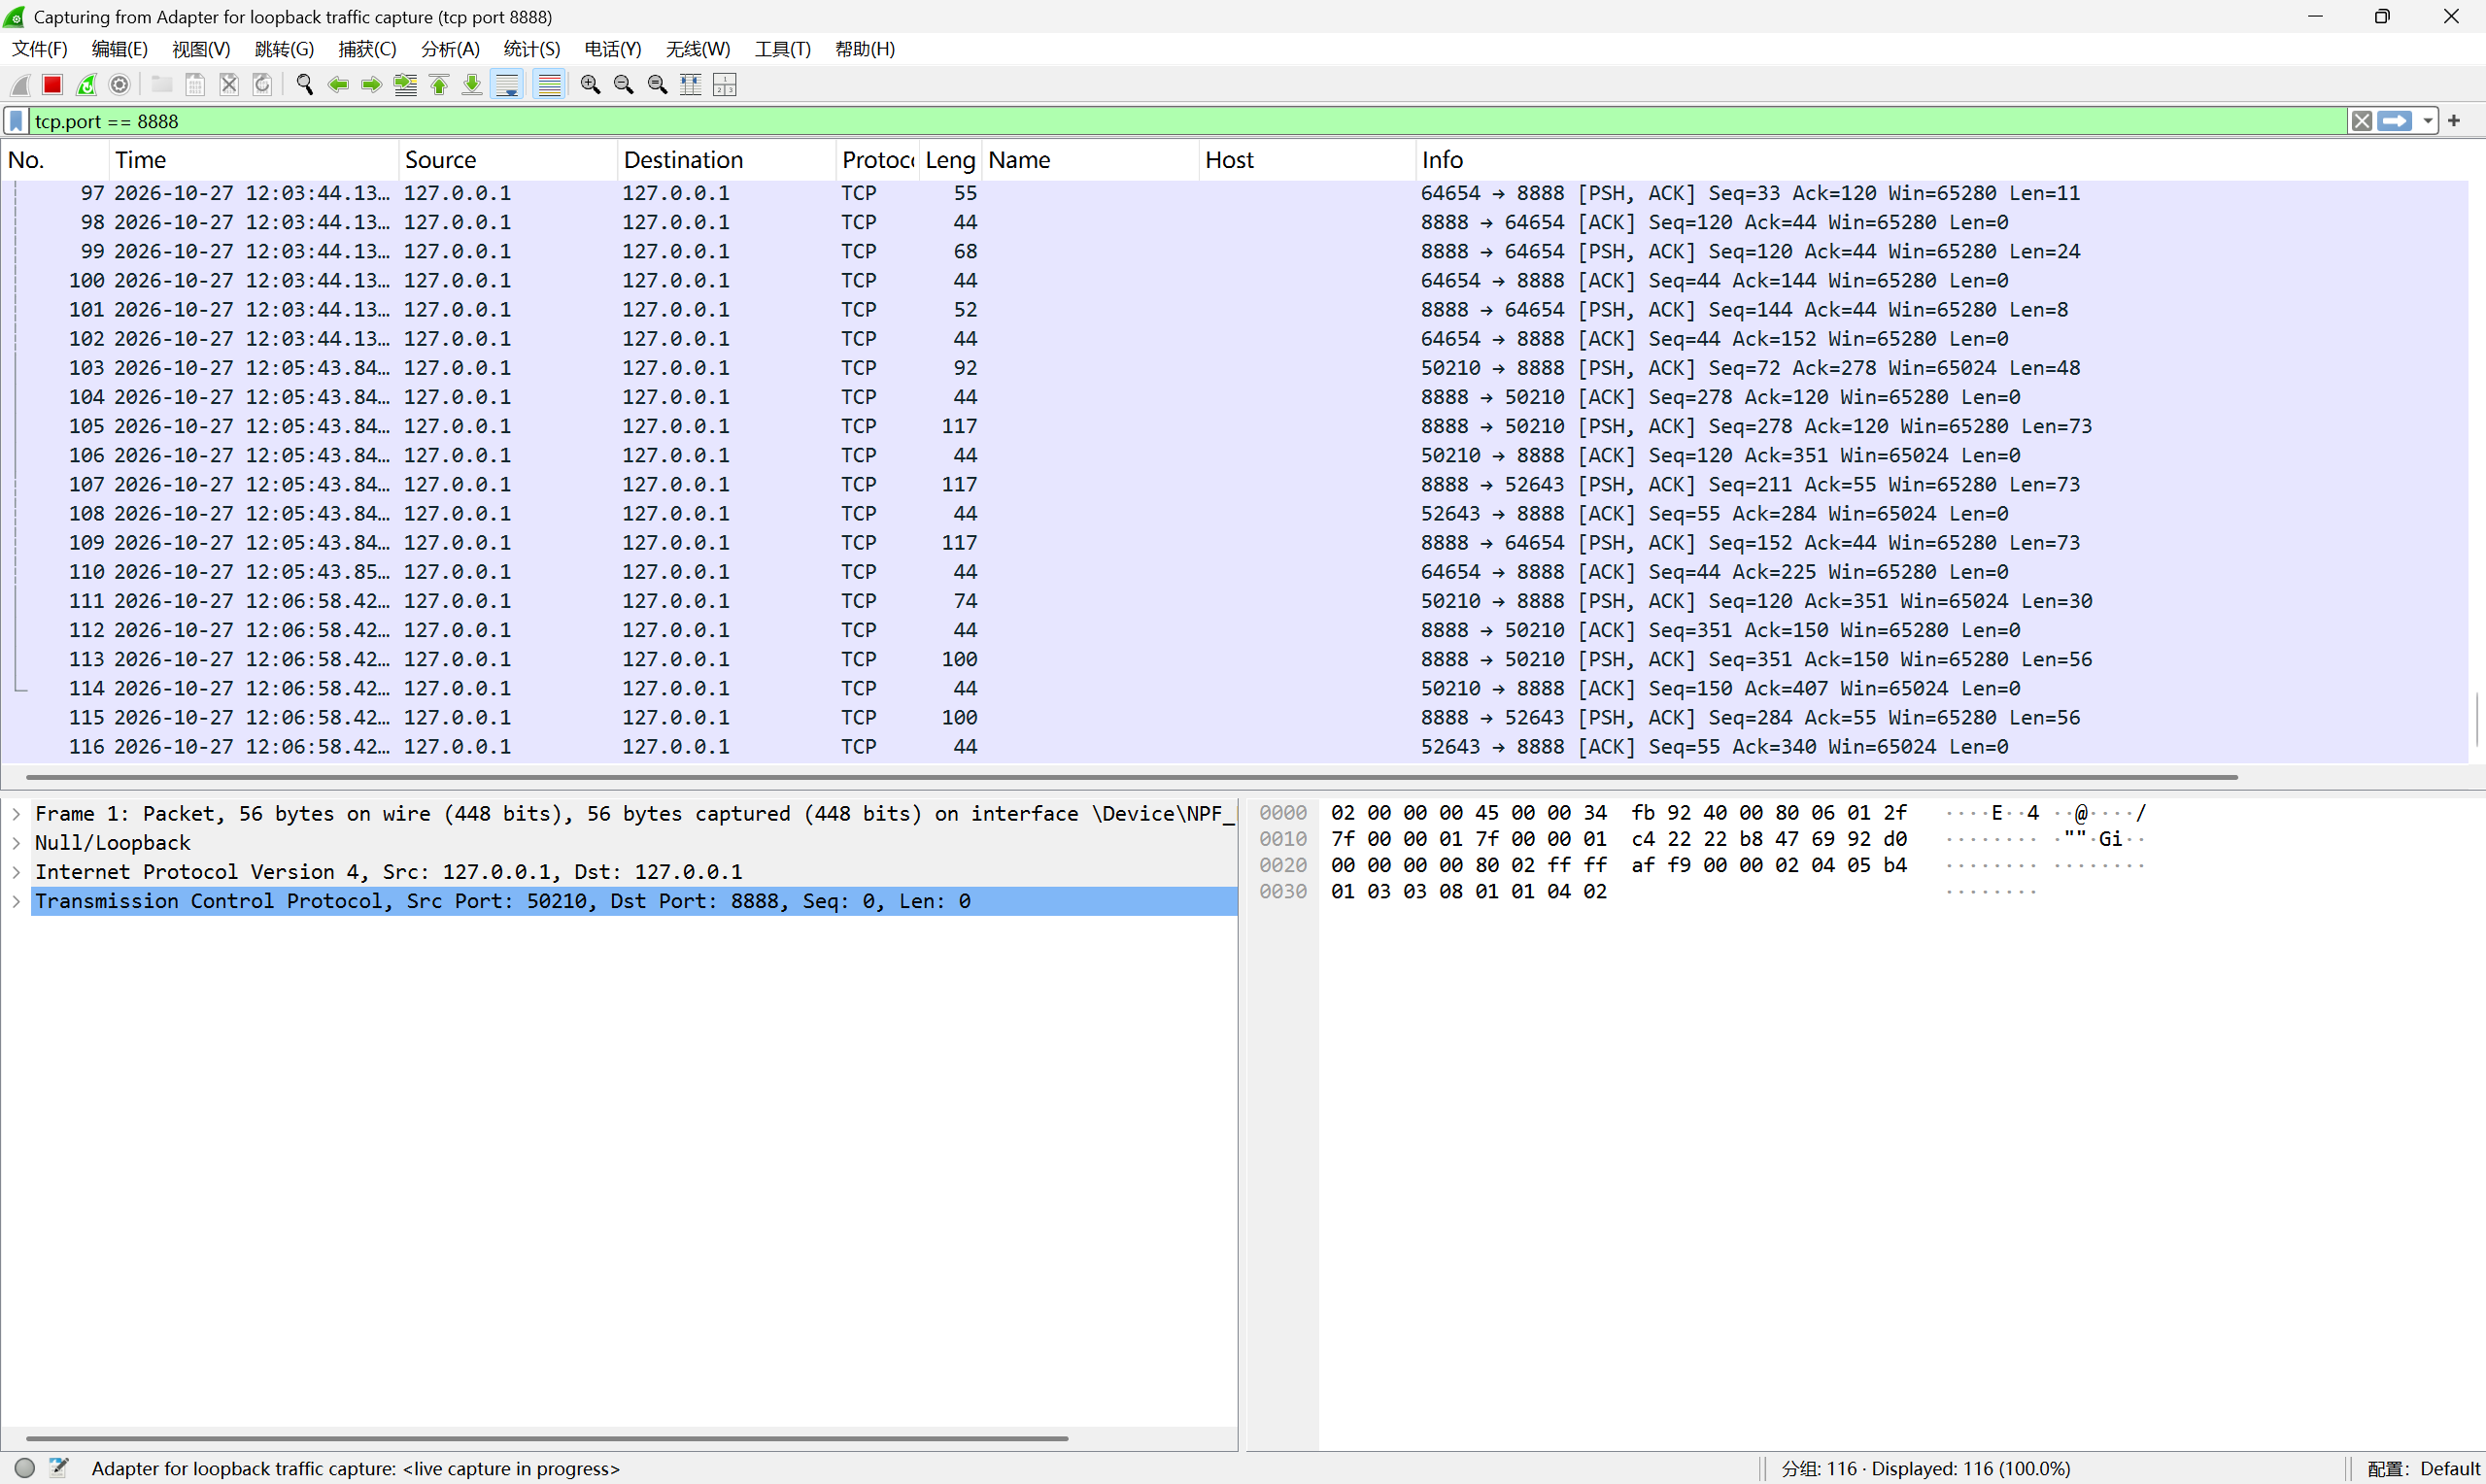
\includegraphics[width=\linewidth,height=10.0cm,keepaspectratio]{images/screen_67.png}
\captionof{figure}{私聊对应的 TCP 流量}\label{fig:s67}
\par\smallskip{\raggedright\setlength{\parindent}{2em}\indent 私聊后新增双向 TCP 数据及确认分组，对应请求、本人回显和目标转发。\par}
\end{minipage}\par\smallskip
\subsection{建群流量}
Alice 建立 Chat1，再依次添加 Bob、Charlie，每次操作后都出现群提示及新增 TCP 数据。解析负载时，可以将这些变化对应到 GROUP、GROUP\_OK 和成员通知。

\par\smallskip\noindent\begin{minipage}{\linewidth}\centering
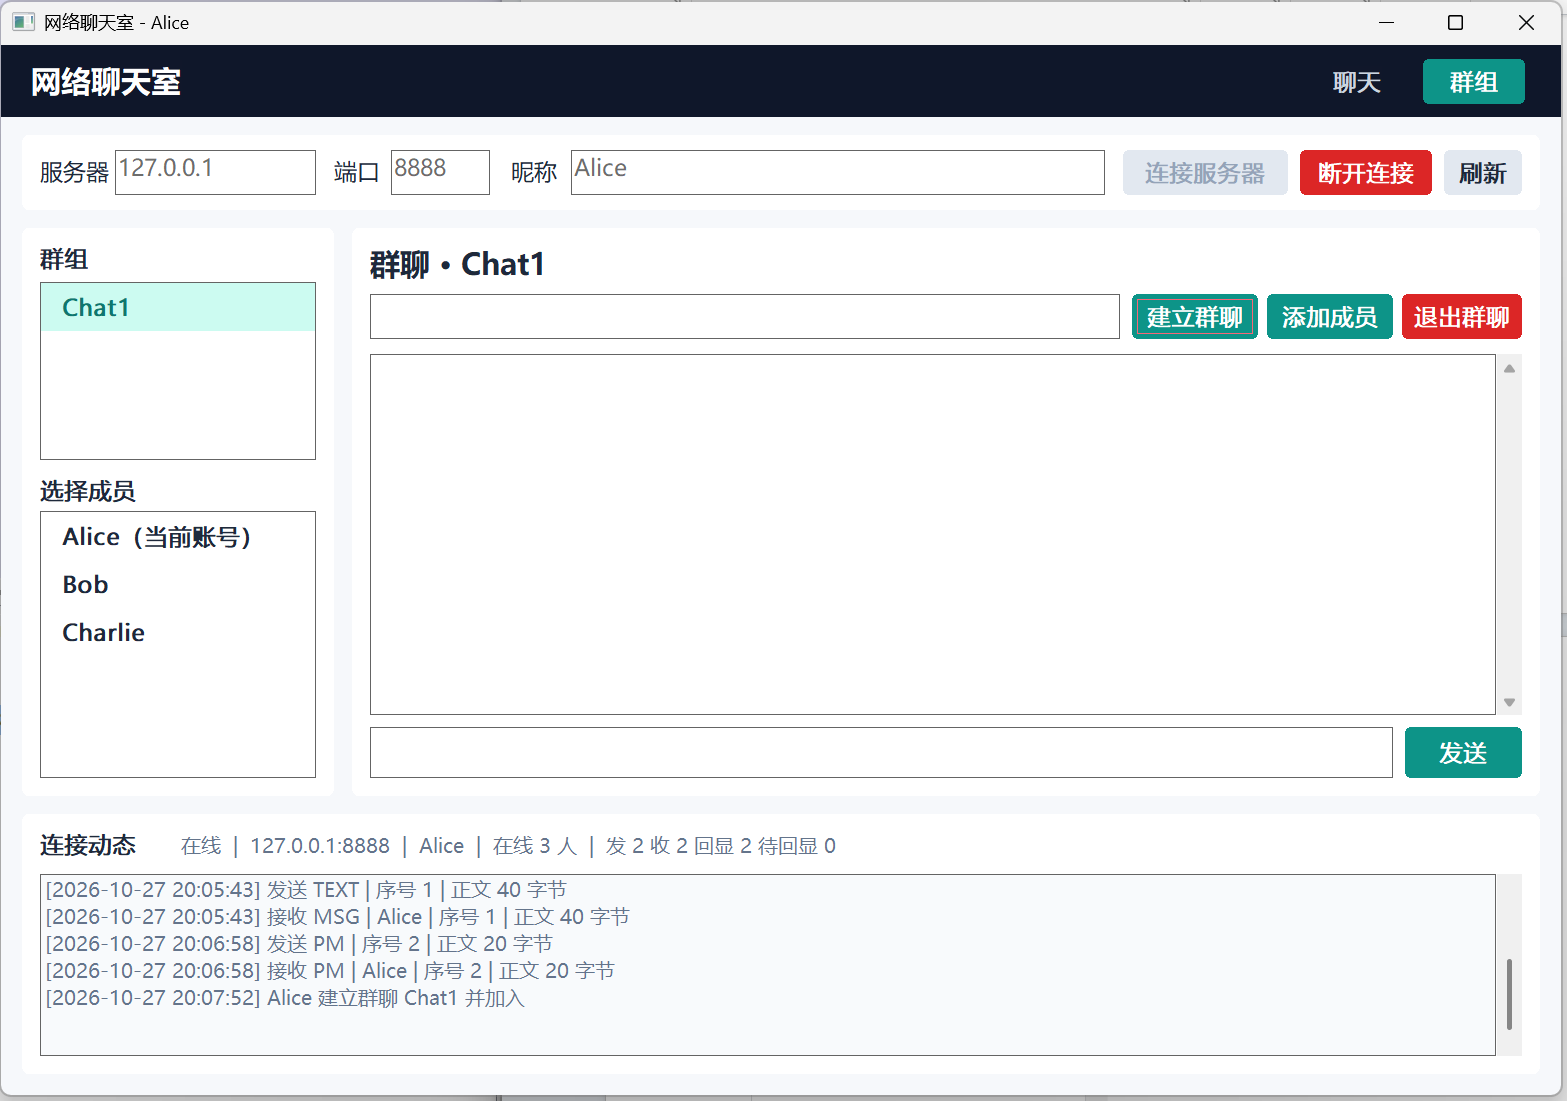
\includegraphics[width=\linewidth,height=10.0cm,keepaspectratio]{images/screen_68.png}
\captionof{figure}{抓包期间建立 Chat1}\label{fig:s68}
\par\smallskip{\raggedright\setlength{\parindent}{2em}\indent 在抓包期间建立 Chat1 后，Alice 底部显示创建成功提示。\par}
\end{minipage}\par\smallskip
\par\smallskip\noindent\begin{minipage}{\linewidth}\centering
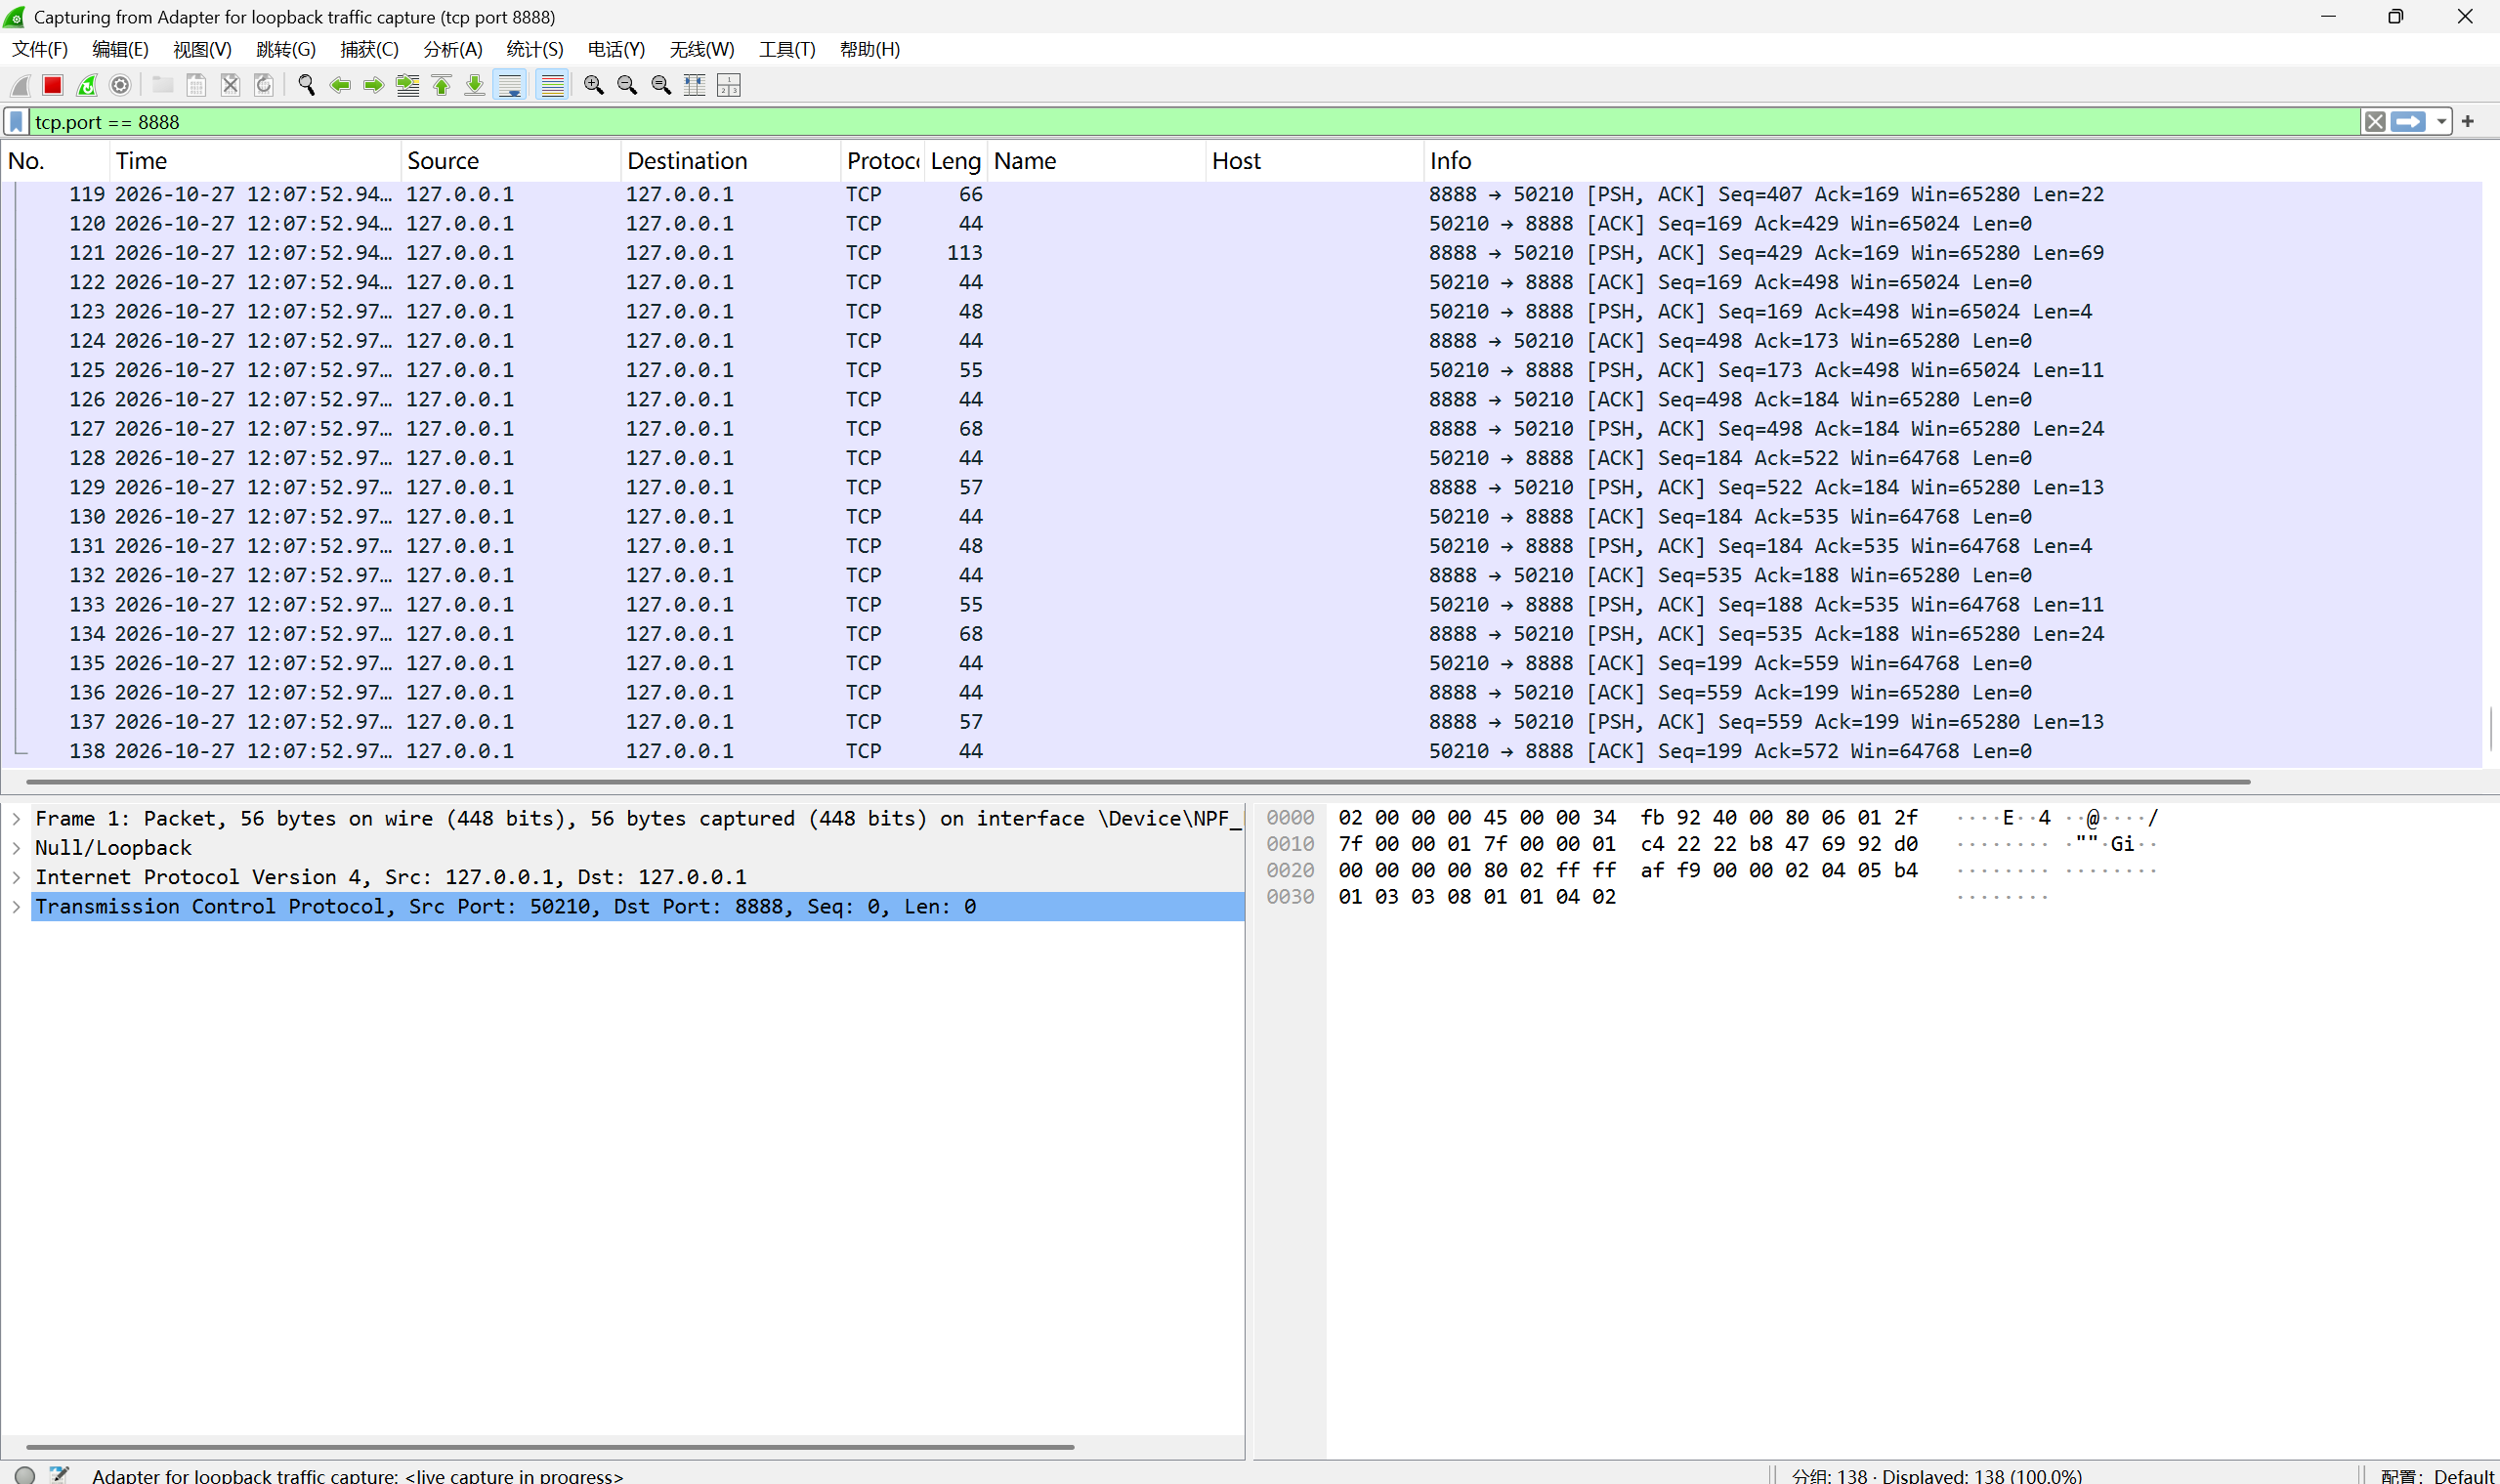
\includegraphics[width=\linewidth,height=10.0cm,keepaspectratio]{images/screen_69.png}
\captionof{figure}{建群对应的 TCP 流量}\label{fig:s69}
\par\smallskip{\raggedright\setlength{\parindent}{2em}\indent 建群后列表继续增加 TCP 数据和 ACK，负载中包含 GROUP 请求及其响应。\par}
\end{minipage}\par\smallskip
\par\smallskip\noindent\begin{minipage}{\linewidth}\centering
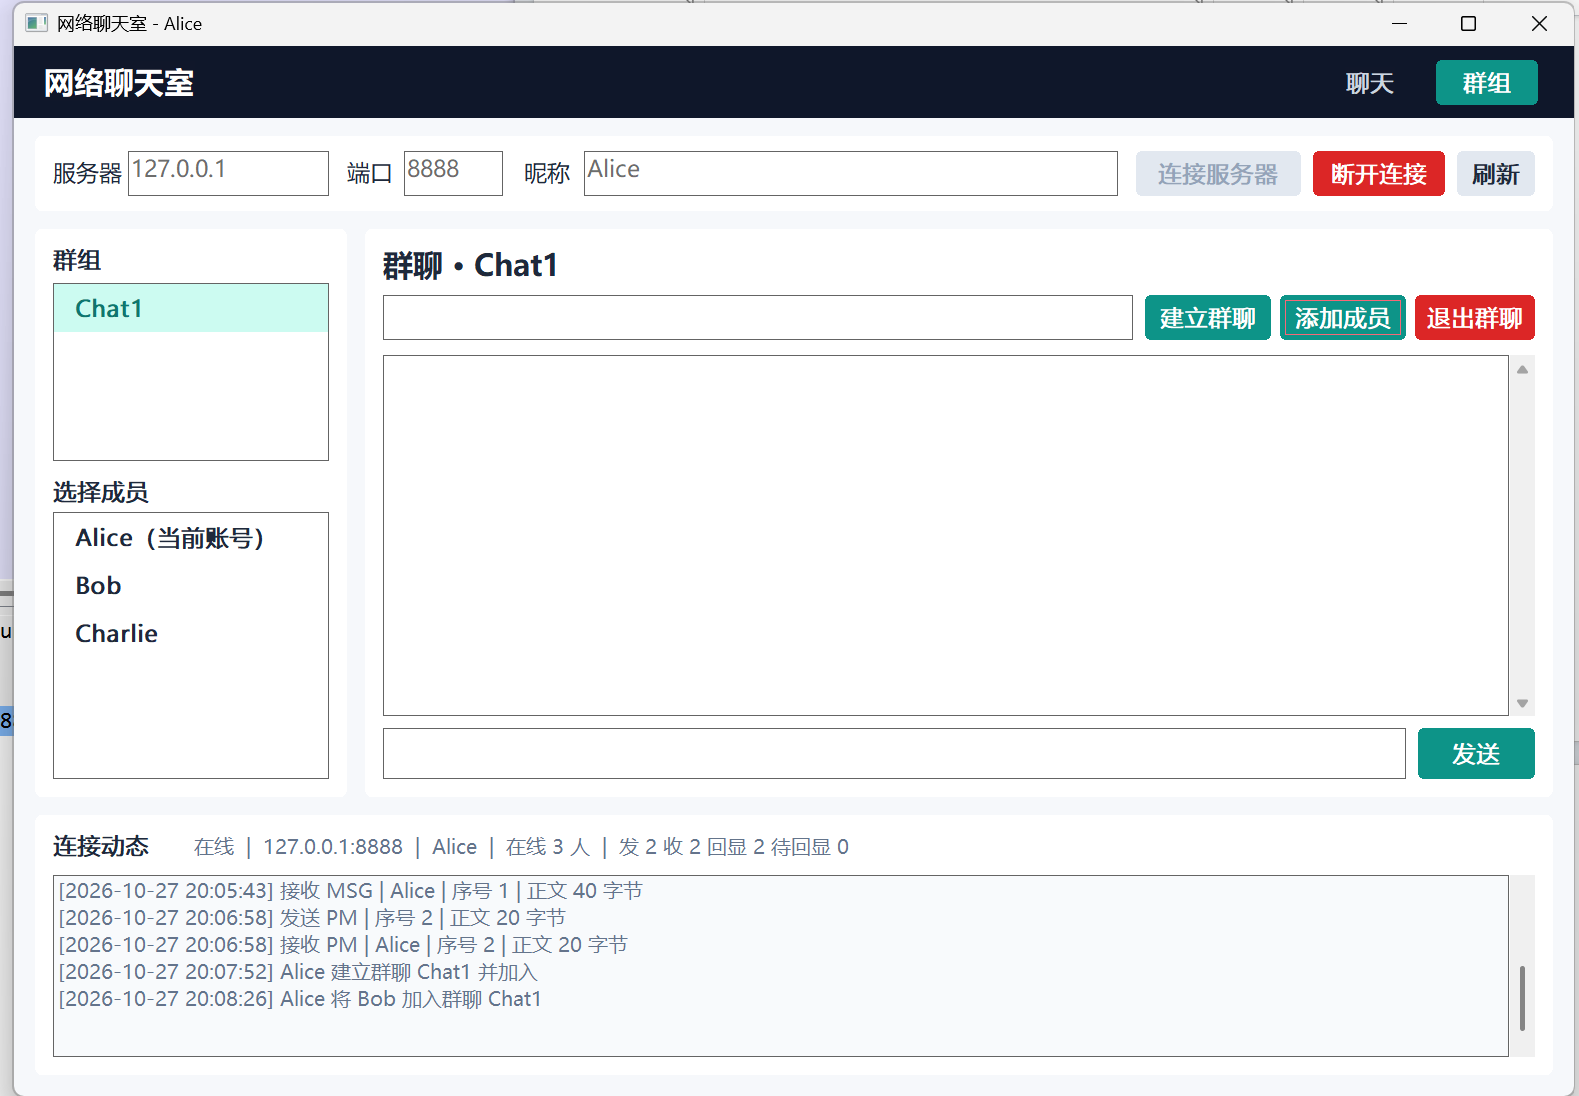
\includegraphics[width=\linewidth,height=10.0cm,keepaspectratio]{images/screen_70.png}
\captionof{figure}{抓包期间添加 Bob}\label{fig:s70}
\par\smallskip{\raggedright\setlength{\parindent}{2em}\indent 添加 Bob 后，Alice 中出现相应入群通知。\par}
\end{minipage}\par\smallskip
\par\smallskip\noindent\begin{minipage}{\linewidth}\centering
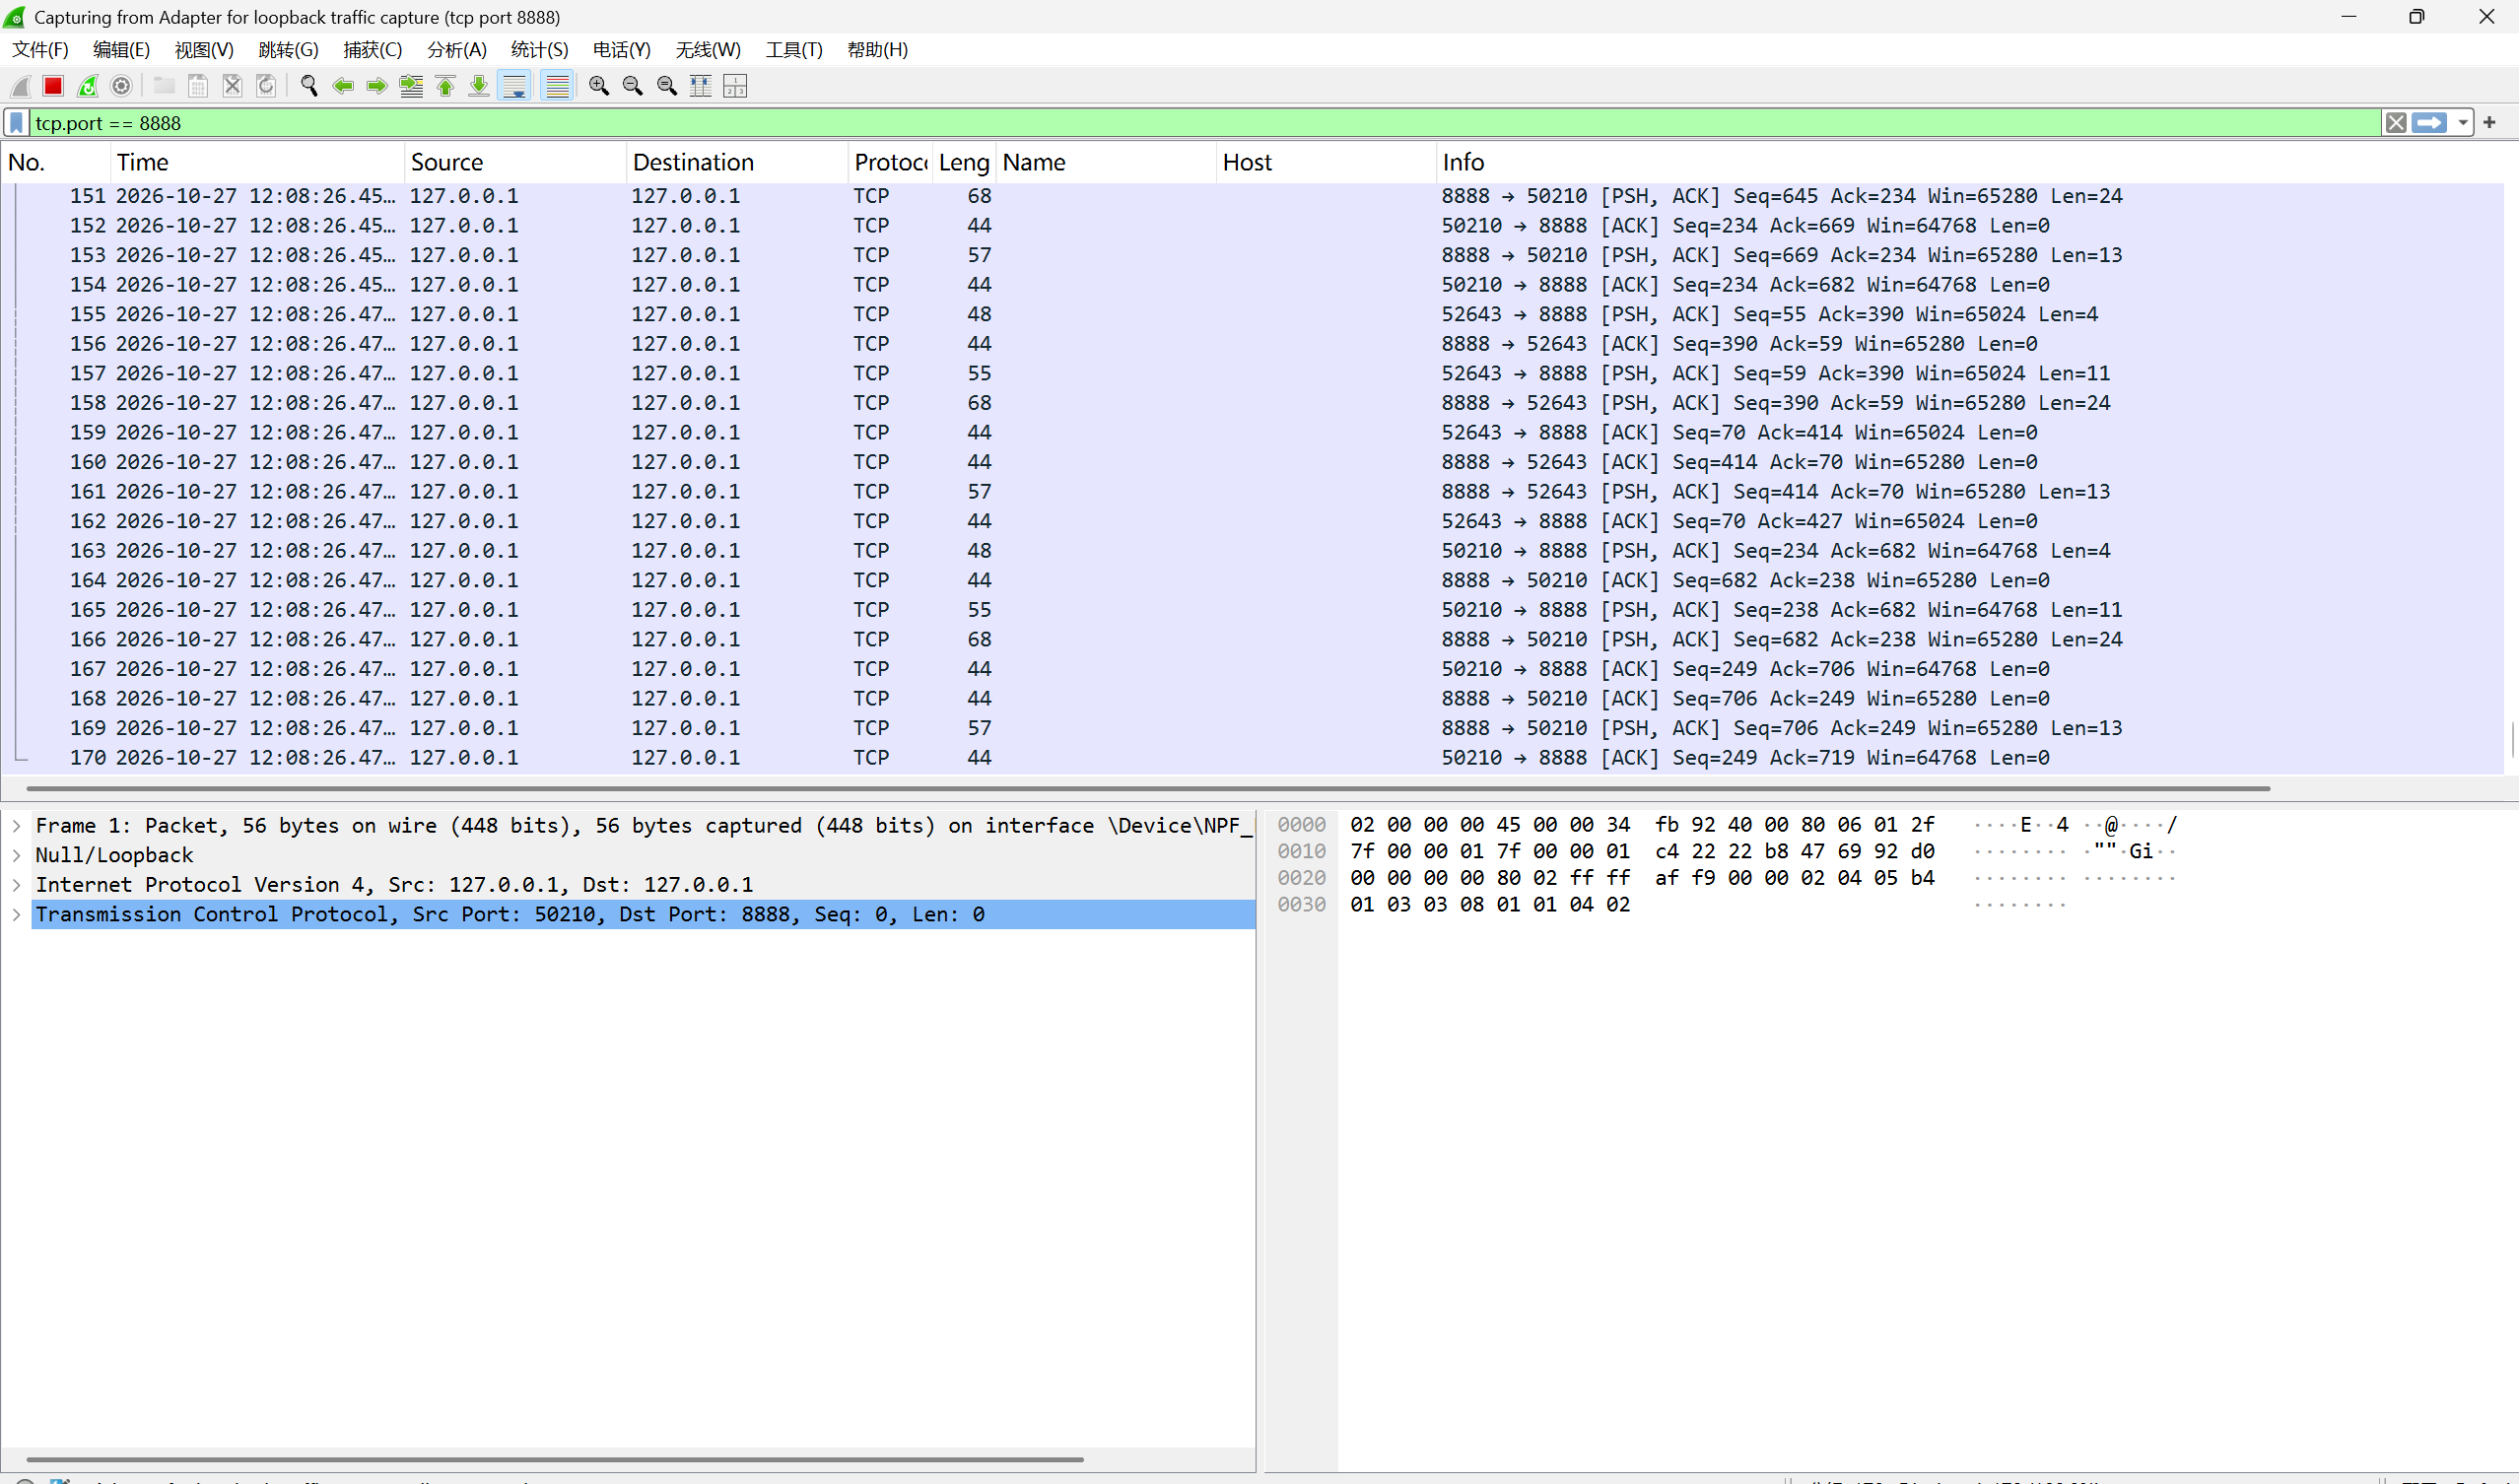
\includegraphics[width=\linewidth,height=10.0cm,keepaspectratio]{images/screen_71.png}
\captionof{figure}{添加 Bob 后的 TCP 流量}\label{fig:s71}
\par\smallskip{\raggedright\setlength{\parindent}{2em}\indent 流量列表随成员增加继续变化，包含添加请求、响应及成员通知的传输。\par}
\end{minipage}\par\smallskip
\par\smallskip\noindent\begin{minipage}{\linewidth}\centering
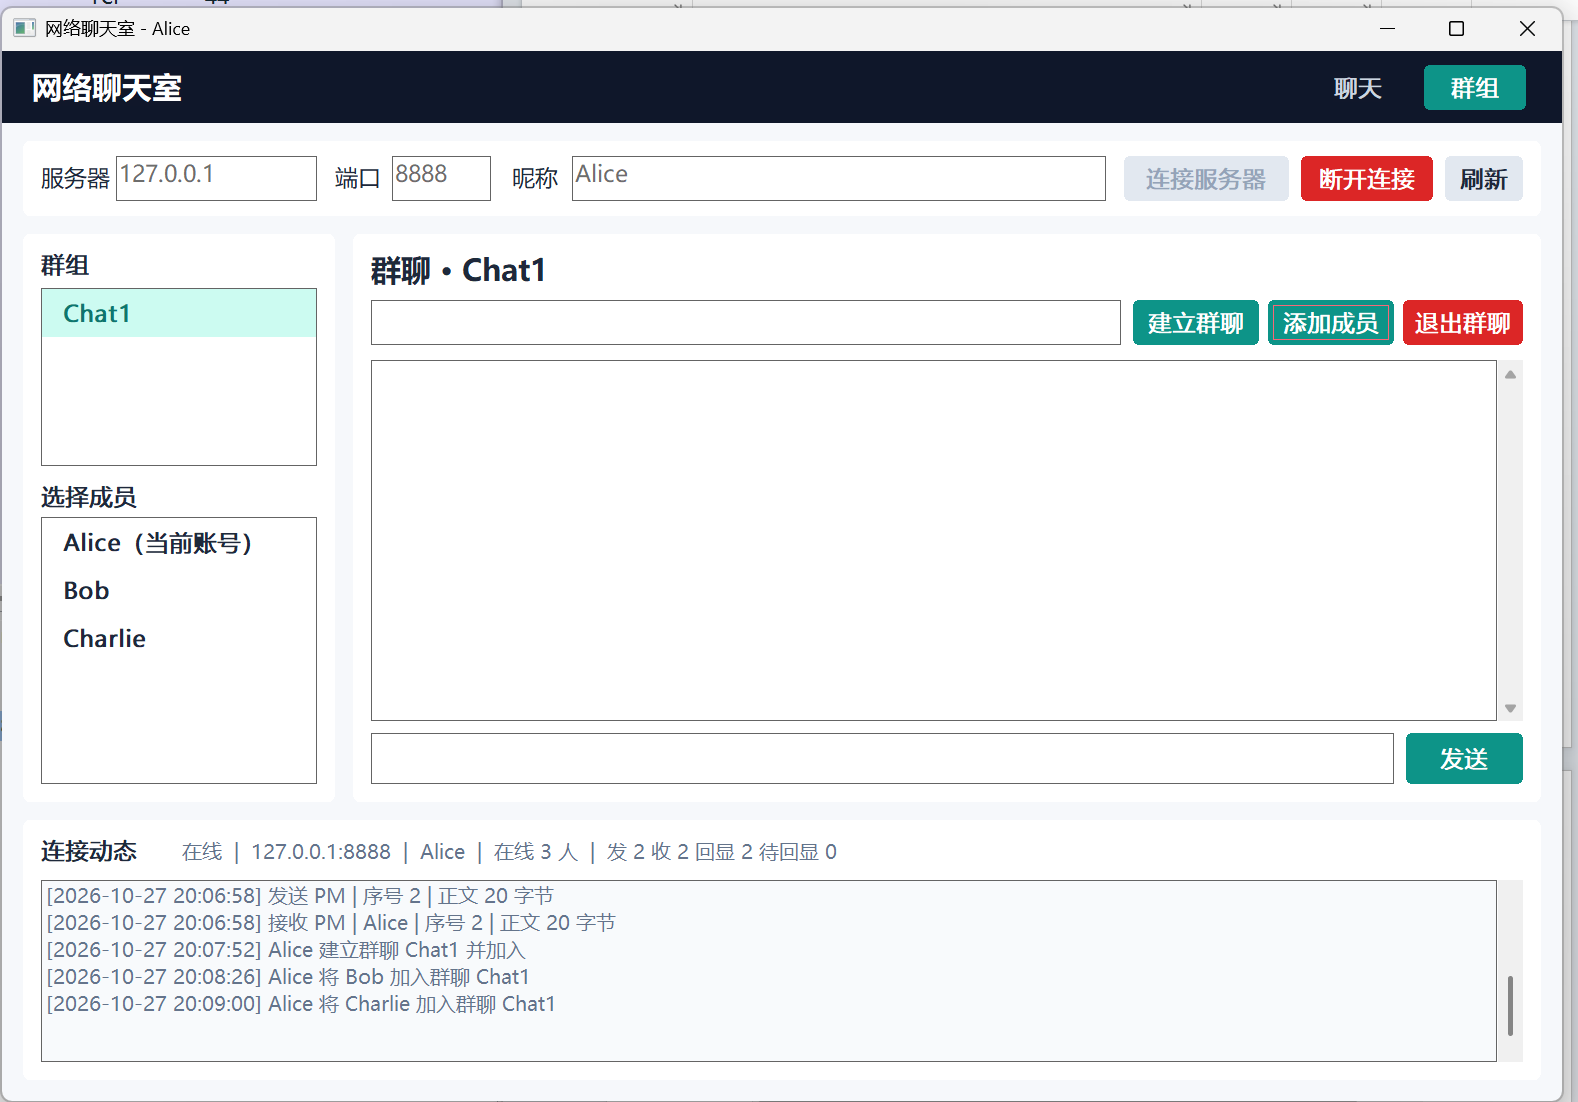
\includegraphics[width=\linewidth,height=10.0cm,keepaspectratio]{images/screen_72.png}
\captionof{figure}{抓包期间添加 Charlie}\label{fig:s72}
\par\smallskip{\raggedright\setlength{\parindent}{2em}\indent 添加 Charlie 后，Chat1 中已经有三位用户，底部记录新的成员提示。\par}
\end{minipage}\par\smallskip
\par\smallskip\noindent\begin{minipage}{\linewidth}\centering
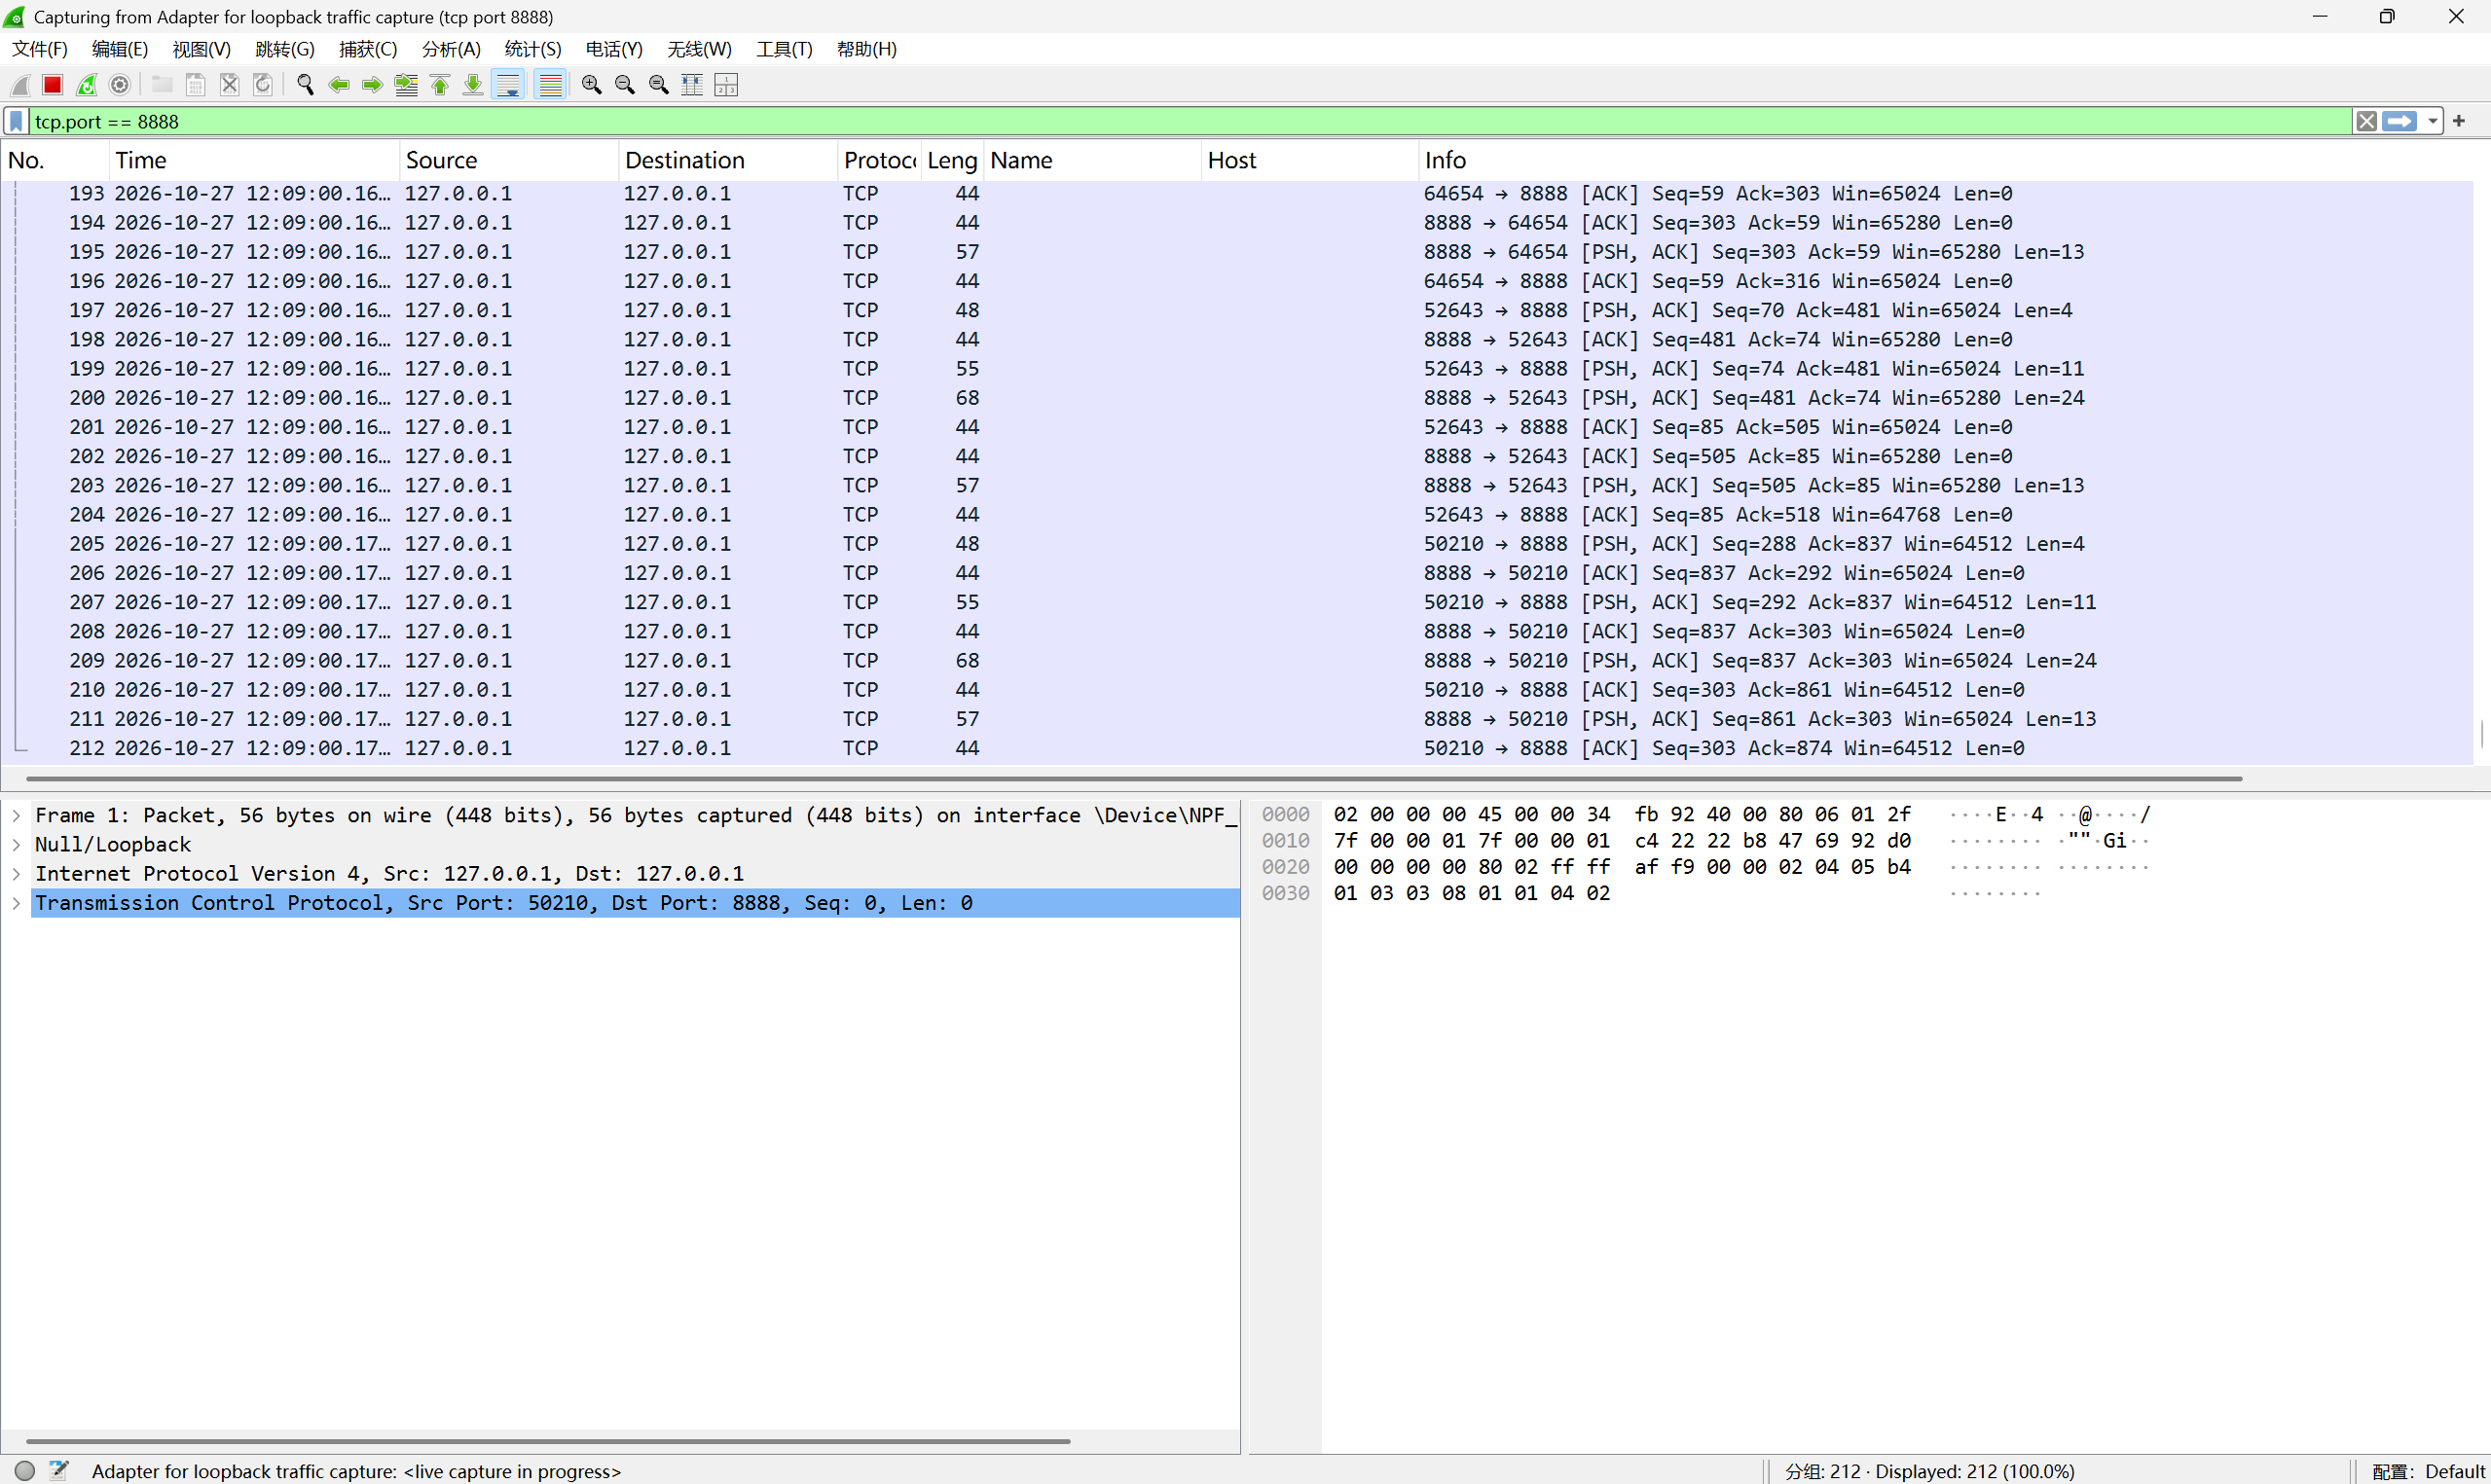
\includegraphics[width=\linewidth,height=10.0cm,keepaspectratio]{images/screen_73.png}
\captionof{figure}{添加 Charlie 后的 TCP 流量}\label{fig:s73}
\par\smallskip{\raggedright\setlength{\parindent}{2em}\indent 此后新增的数据对应 Charlie 的成员变更，使这一操作也保存在抓包中。\par}
\end{minipage}\par\smallskip
\subsection{群消息流量}
Alice 在 Chat1 输入“大家好，Hello group!”后，三位群成员都接收到 GMSG，第 213 帧记录对应 GTEXT|\allowbreak{}3|\allowbreak{}Chat1。随后 Bob 回复“hello晚上好1111”，第 229 帧记录这条群请求。

\par\smallskip\noindent\begin{minipage}{\linewidth}\centering
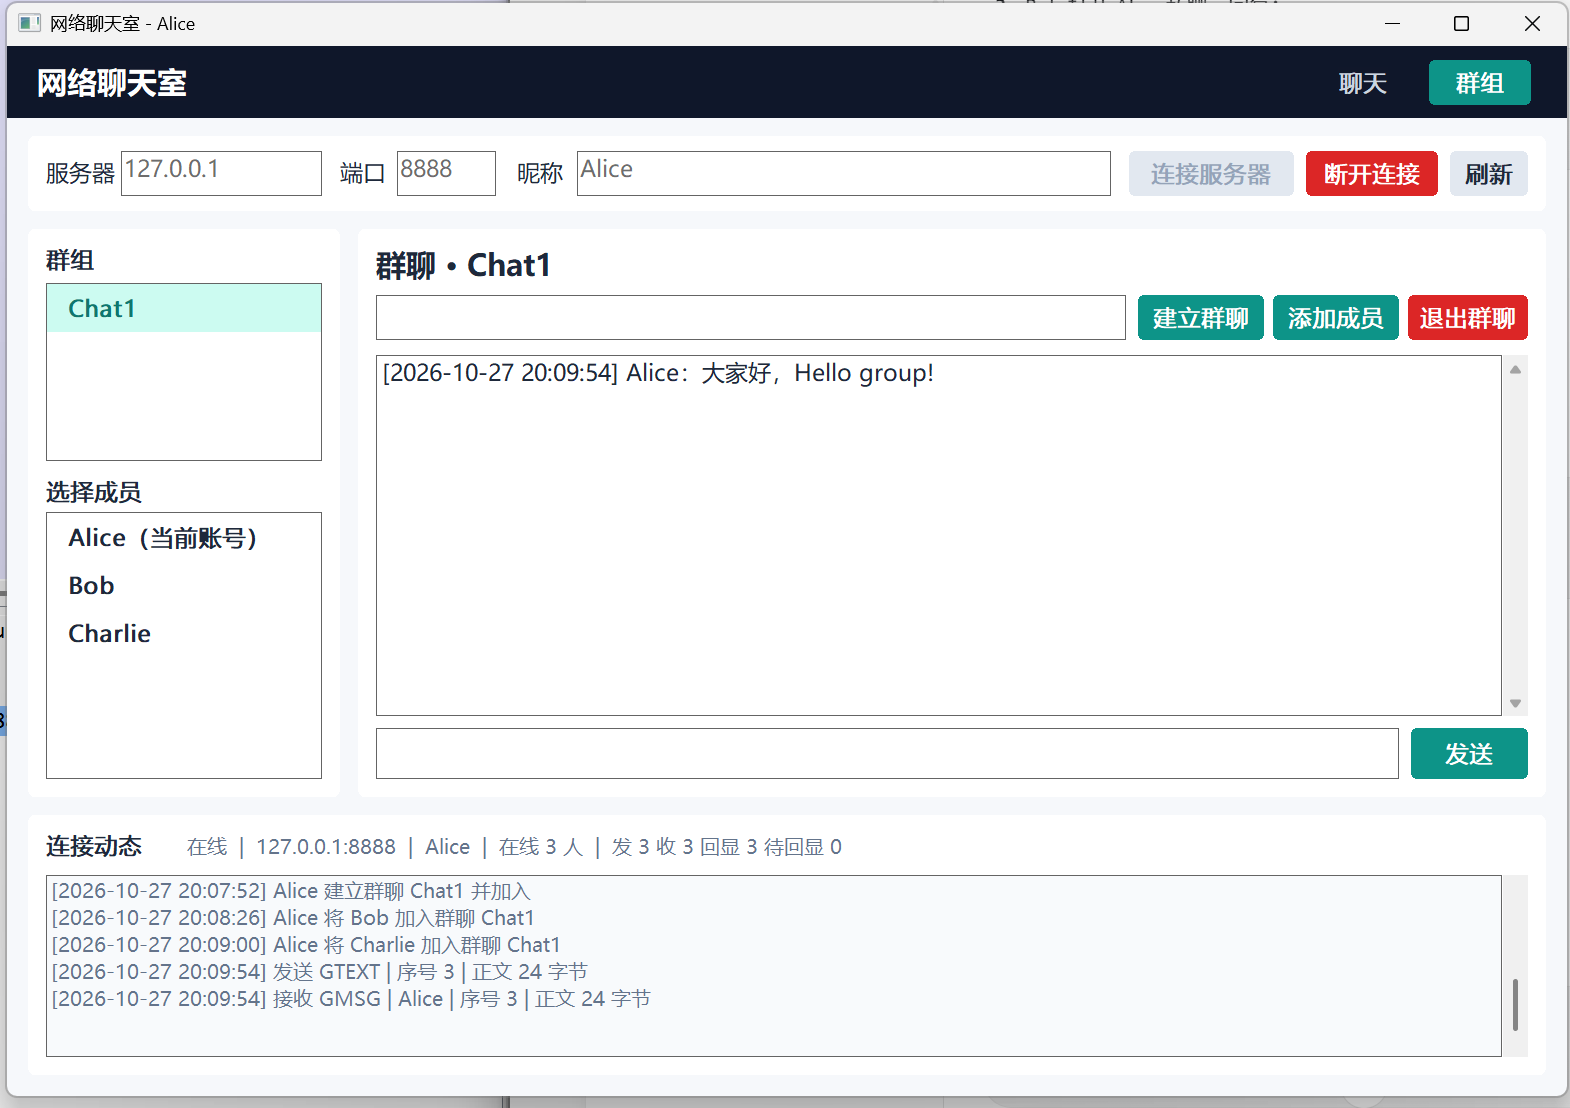
\includegraphics[width=\linewidth,height=10.0cm,keepaspectratio]{images/screen_74.png}
\captionof{figure}{抓包期间 Alice 的群发言}\label{fig:s74}
\par\smallskip{\raggedright\setlength{\parindent}{2em}\indent Alice 发送“大家好，Hello group!”后，群会话出现正文，下方记录 GMSG 回显。\par}
\end{minipage}\par\smallskip
\par\smallskip\noindent\begin{minipage}{\linewidth}\centering
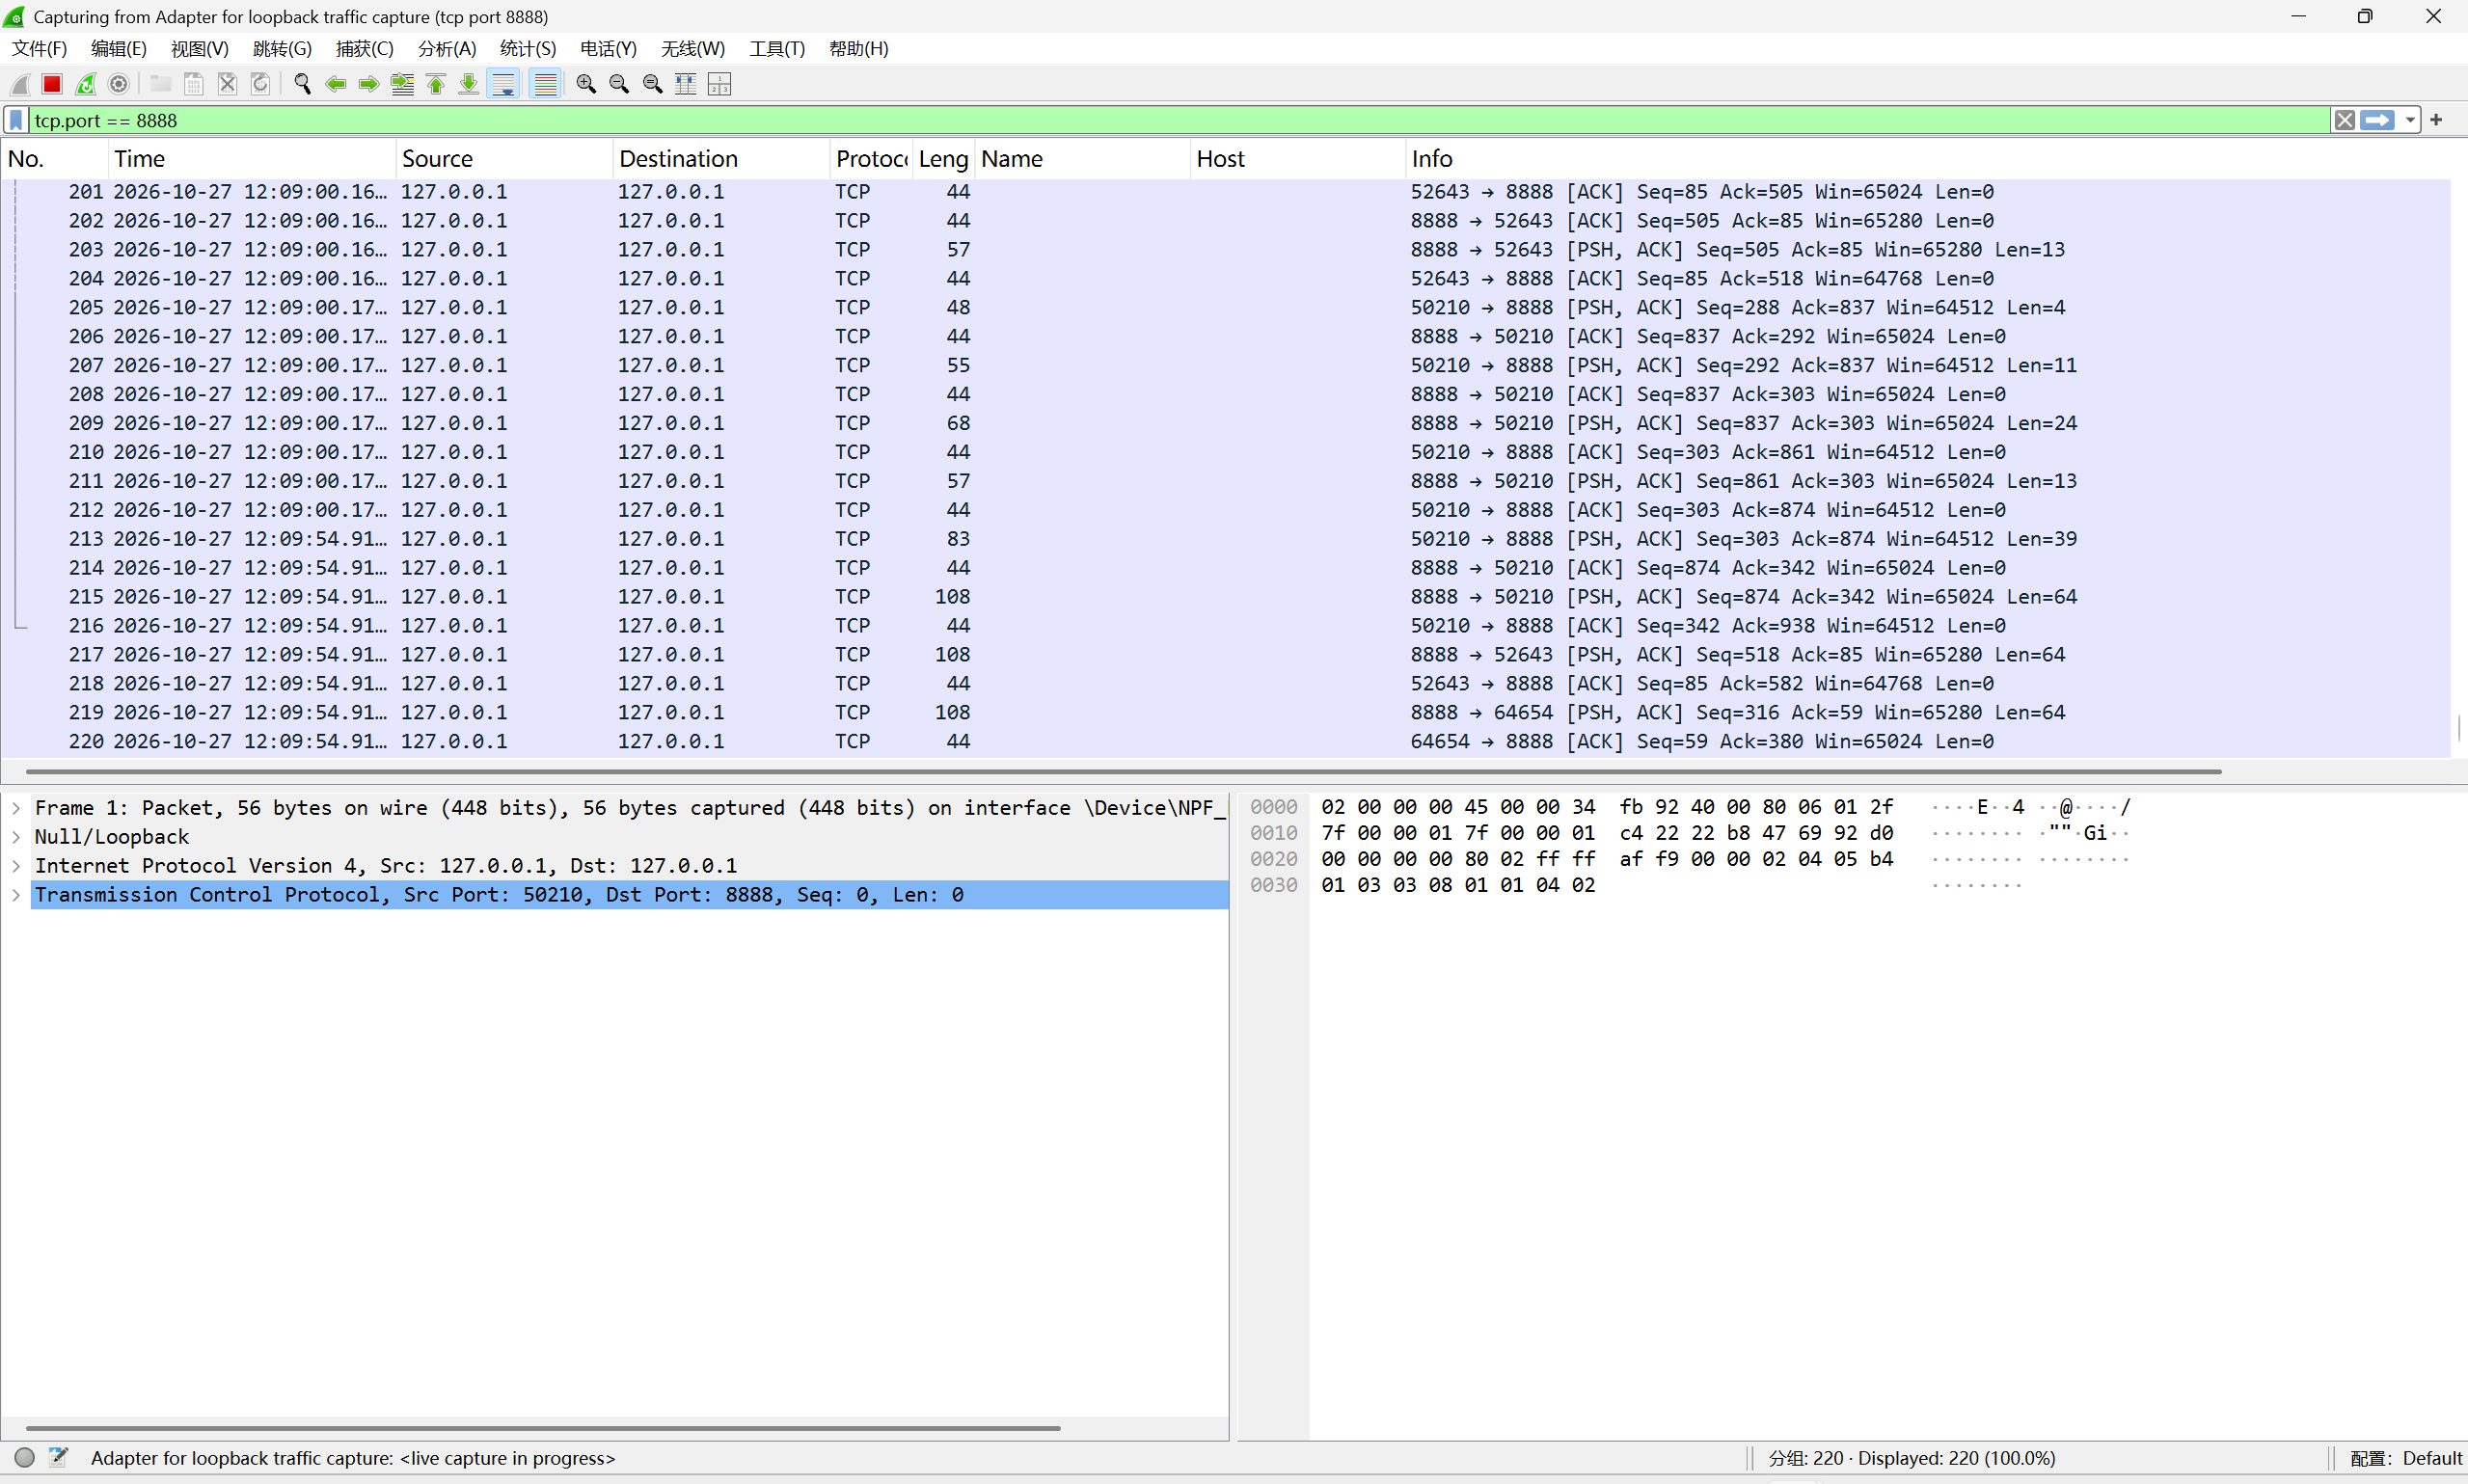
\includegraphics[width=\linewidth,height=10.0cm,keepaspectratio]{images/screen_75.png}
\captionof{figure}{群发言对应的 TCP 流量}\label{fig:s75}
\par\smallskip{\raggedright\setlength{\parindent}{2em}\indent 群发后出现面向三条连接的数据，完整负载中可以分别找到当前成员收到的 GMSG。\par}
\end{minipage}\par\smallskip
\par\smallskip\noindent\begin{minipage}{\linewidth}\centering
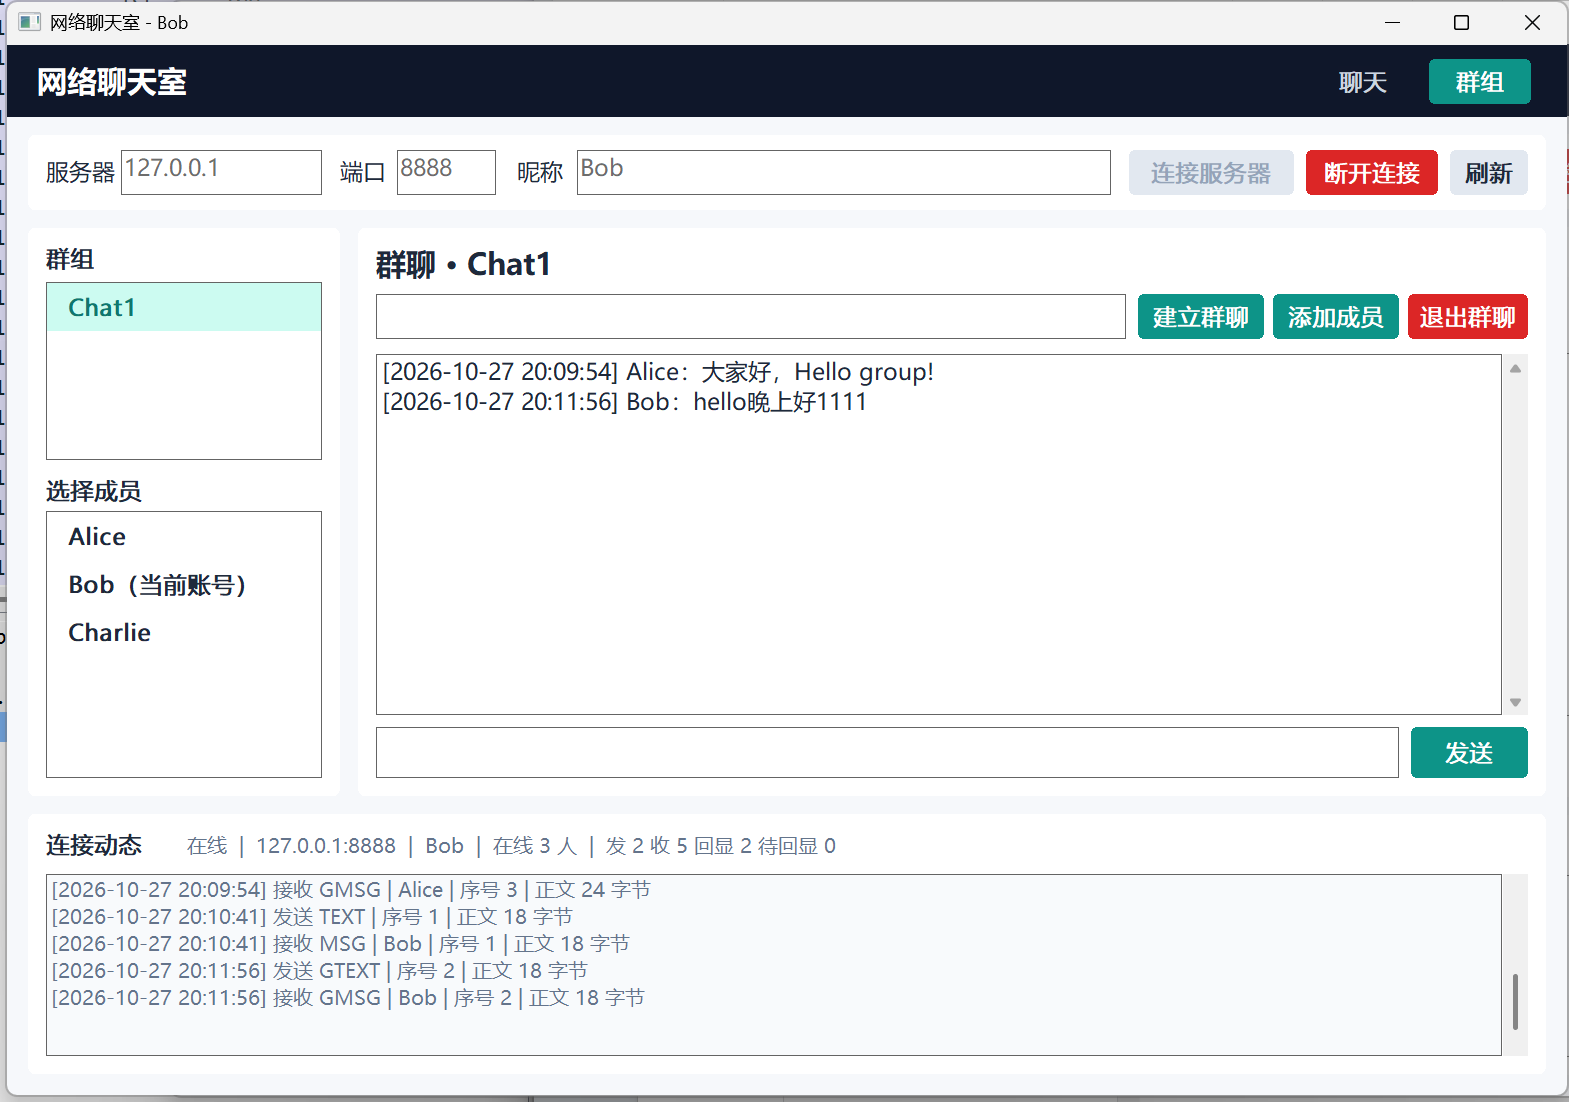
\includegraphics[width=\linewidth,height=10.0cm,keepaspectratio]{images/screen_76.png}
\captionof{figure}{抓包期间 Bob 的群回复}\label{fig:s76}
\par\smallskip{\raggedright\setlength{\parindent}{2em}\indent Bob 回复中英文群消息，底部同时呈现 GTEXT 发送和 GMSG 回显。\par}
\end{minipage}\par\smallskip
\par\smallskip\noindent\begin{minipage}{\linewidth}\centering
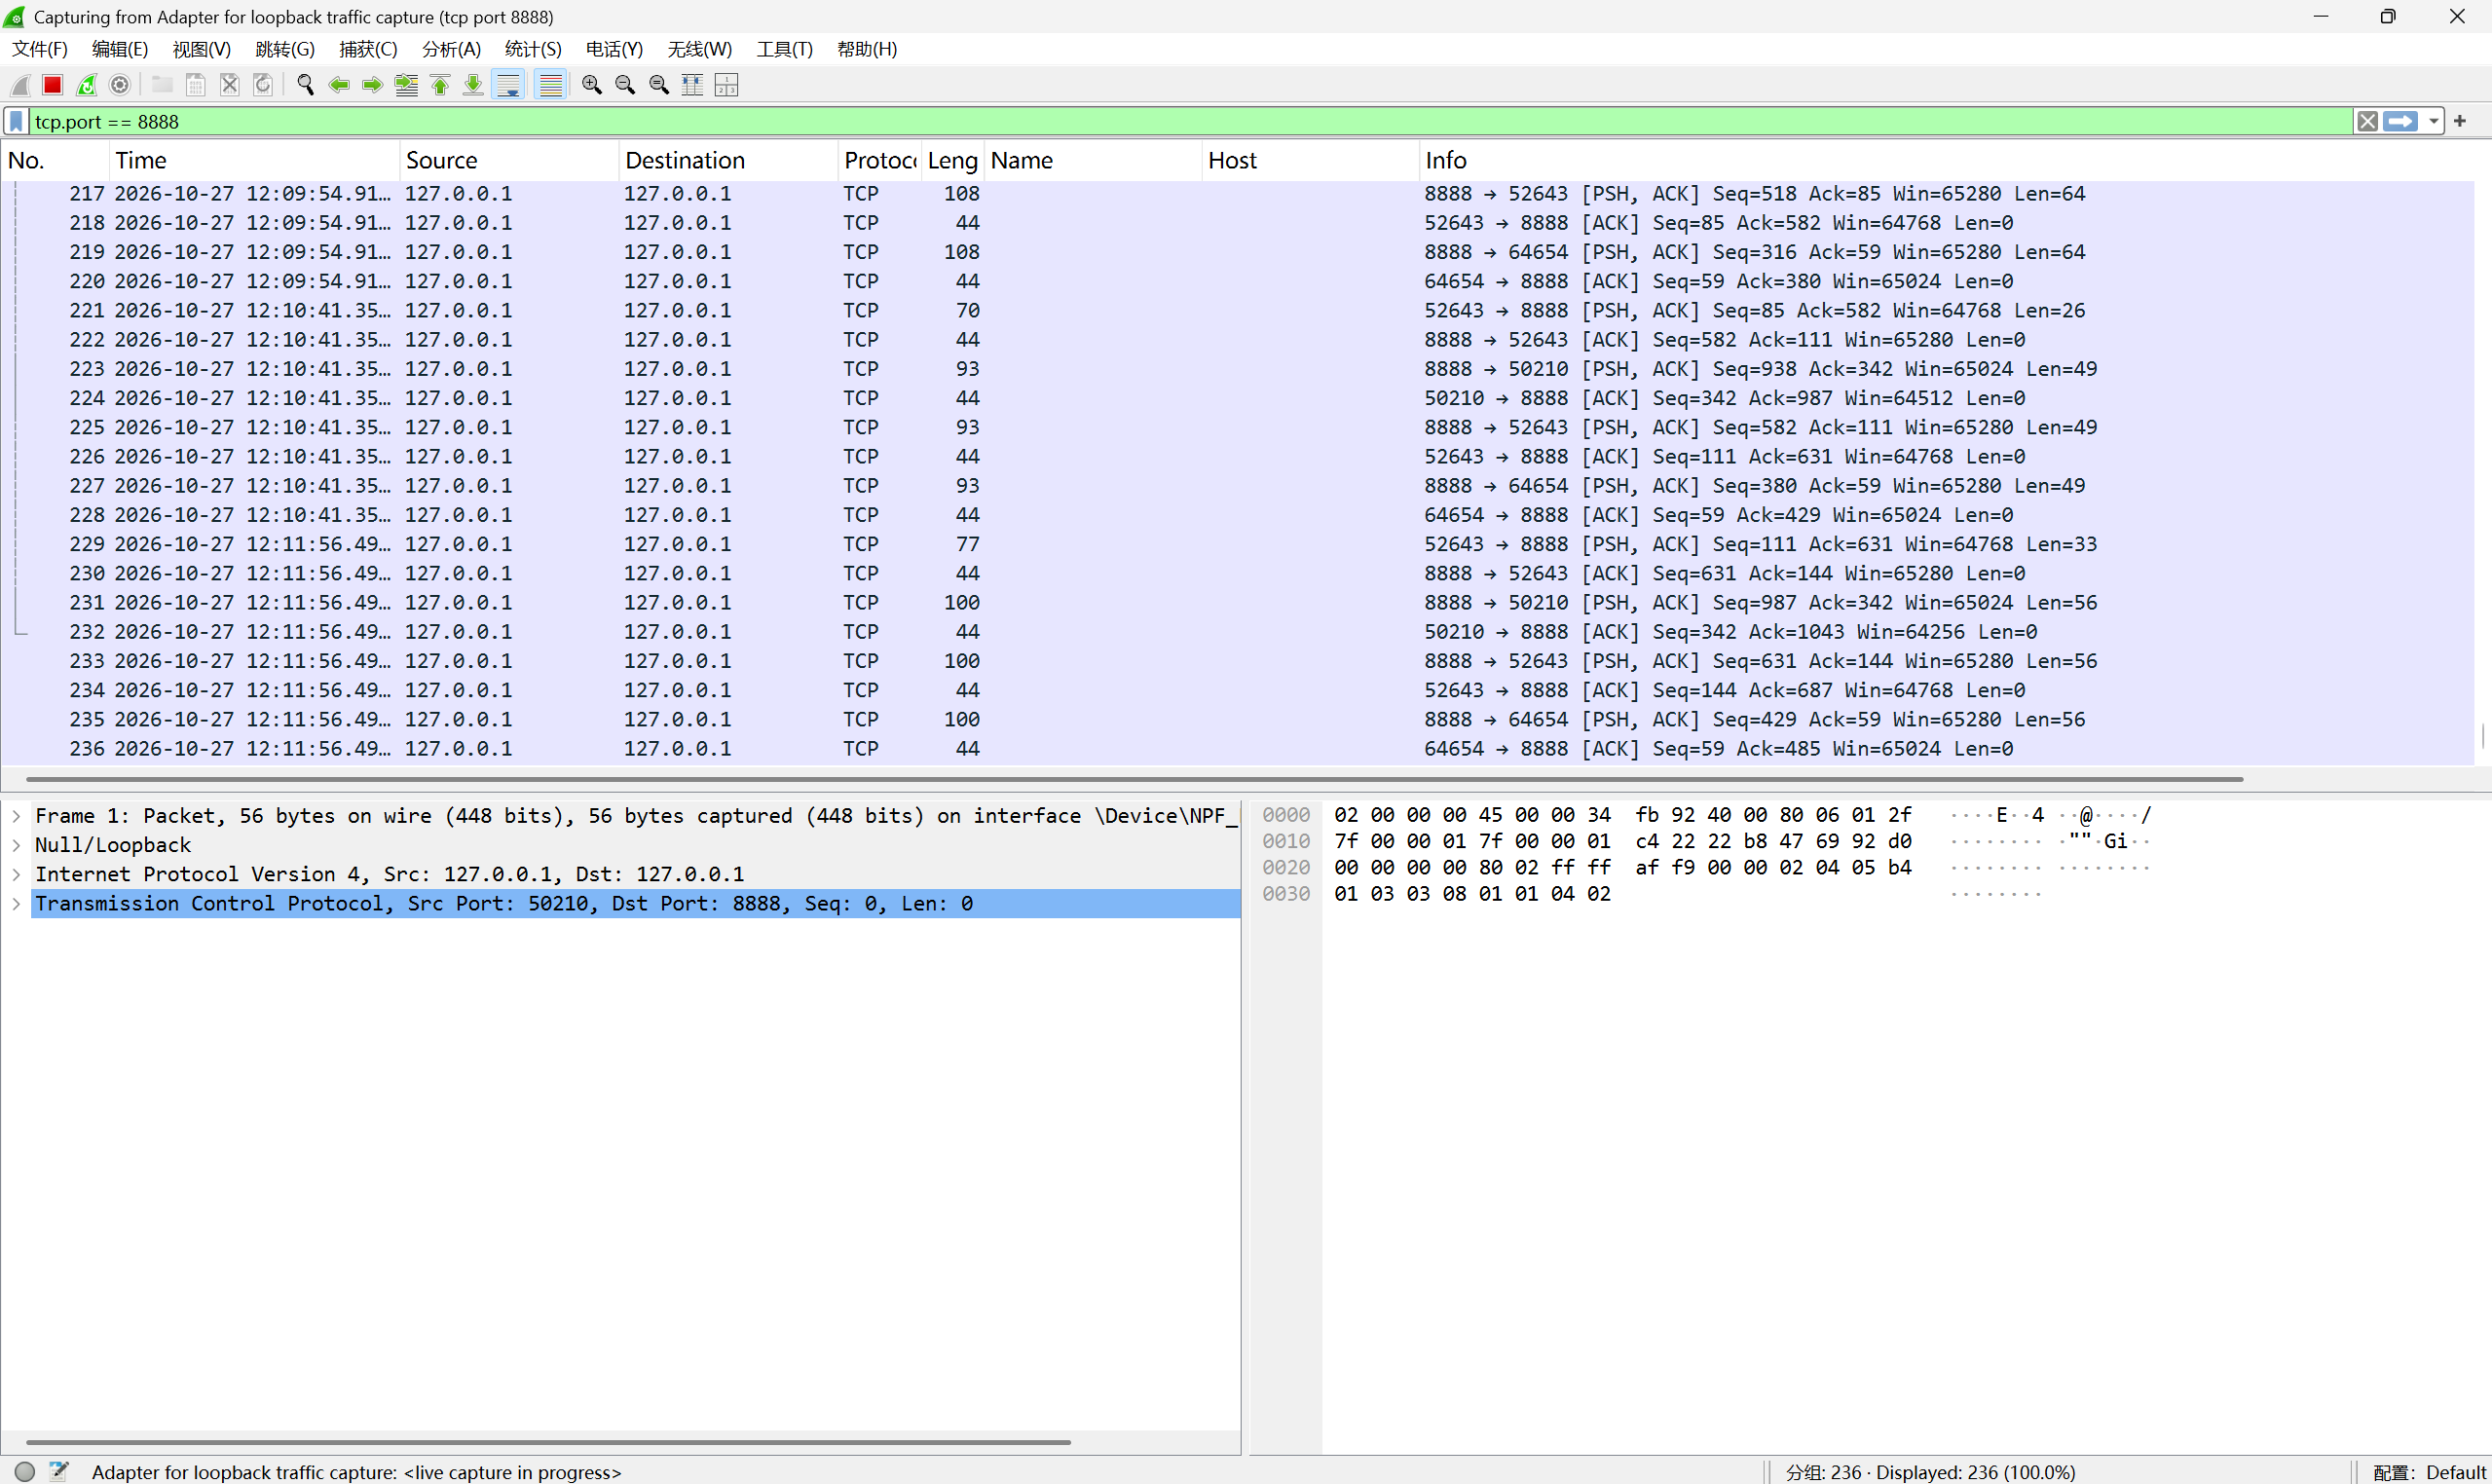
\includegraphics[width=\linewidth,height=10.0cm,keepaspectratio]{images/screen_77.png}
\captionof{figure}{群回复对应的 TCP 流量}\label{fig:s77}
\par\smallskip{\raggedright\setlength{\parindent}{2em}\indent 对应流量继续增加，重组后可以找到 Bob 发言及服务器群转发。\par}
\end{minipage}\par\smallskip
同一抓包中还包含 Bob 的公共消息“hello早上好1111”，对应第 221 帧。公聊、群聊在该连接上继续使用递增序号，但分别按各自类型选择接收集合。

\subsection{退群流量}
Charlie 退出 Chat1 后，客户端显示退出成功，抓包中新增退群请求和成员通知；捕获保持运行，随后继续断开及重新登录。

\par\smallskip\noindent\begin{minipage}{\linewidth}\centering
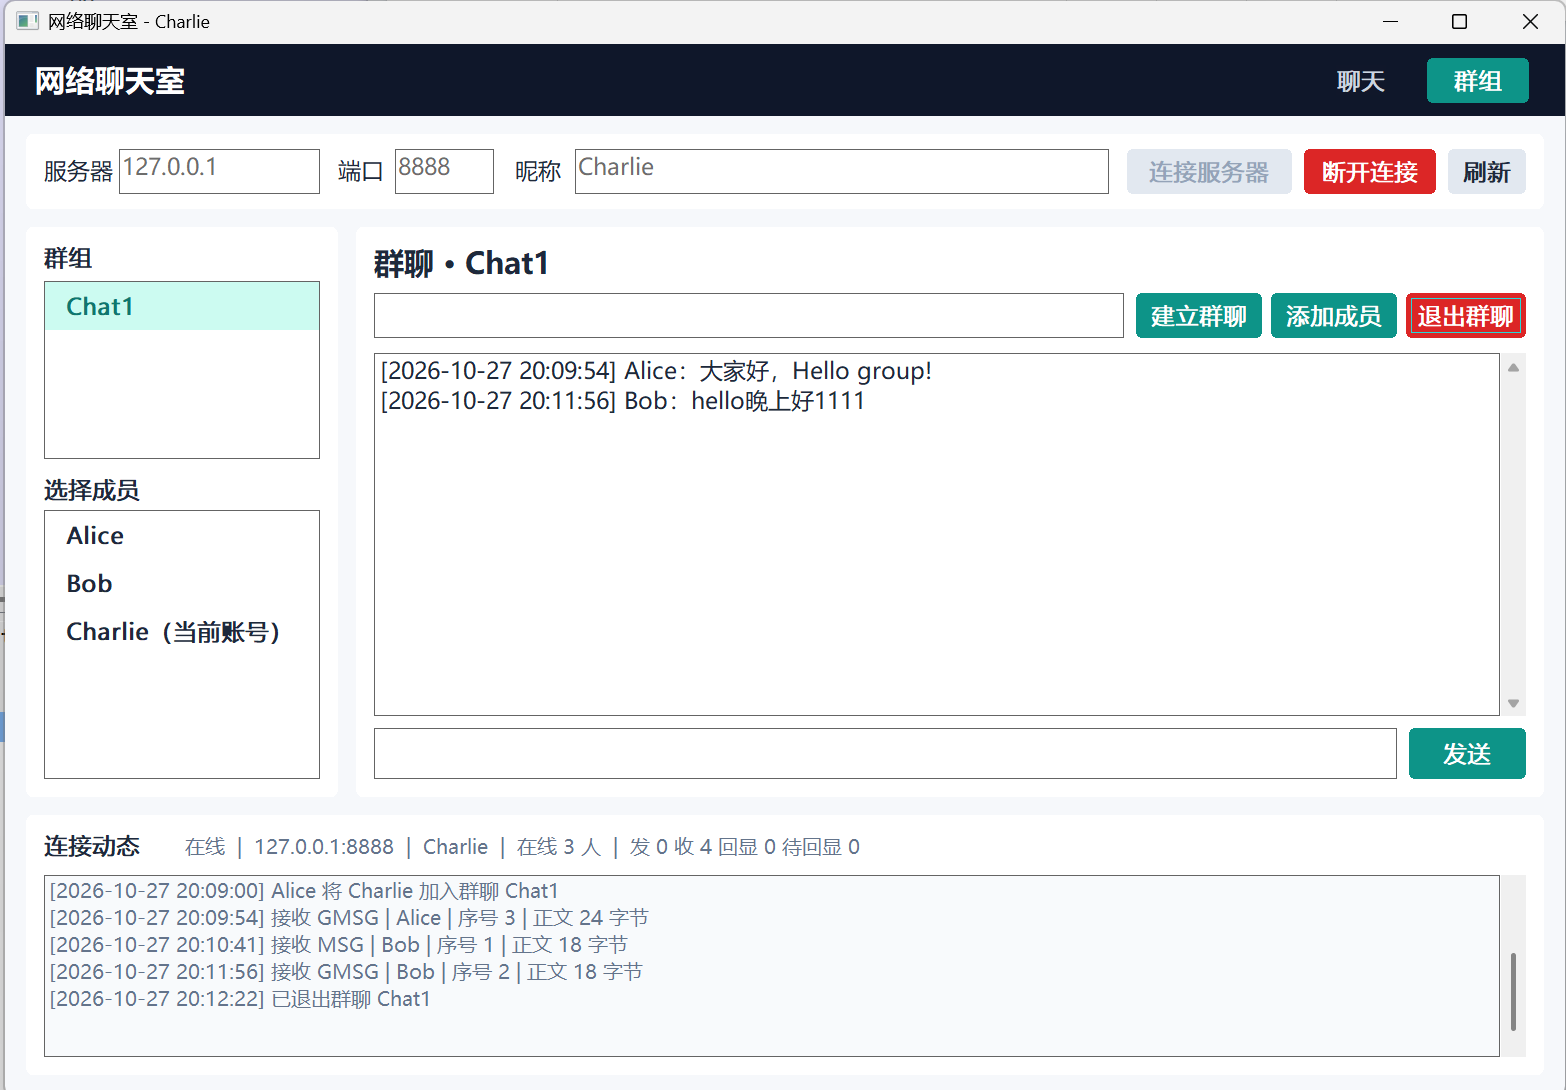
\includegraphics[width=\linewidth,height=10.0cm,keepaspectratio]{images/screen_78.png}
\captionof{figure}{抓包期间 Charlie 退群}\label{fig:s78}
\par\smallskip{\raggedright\setlength{\parindent}{2em}\indent Charlie 退出 Chat1 后，底部显示退群成功，页面保留之前收到的群正文。\par}
\end{minipage}\par\smallskip
\par\smallskip\noindent\begin{minipage}{\linewidth}\centering
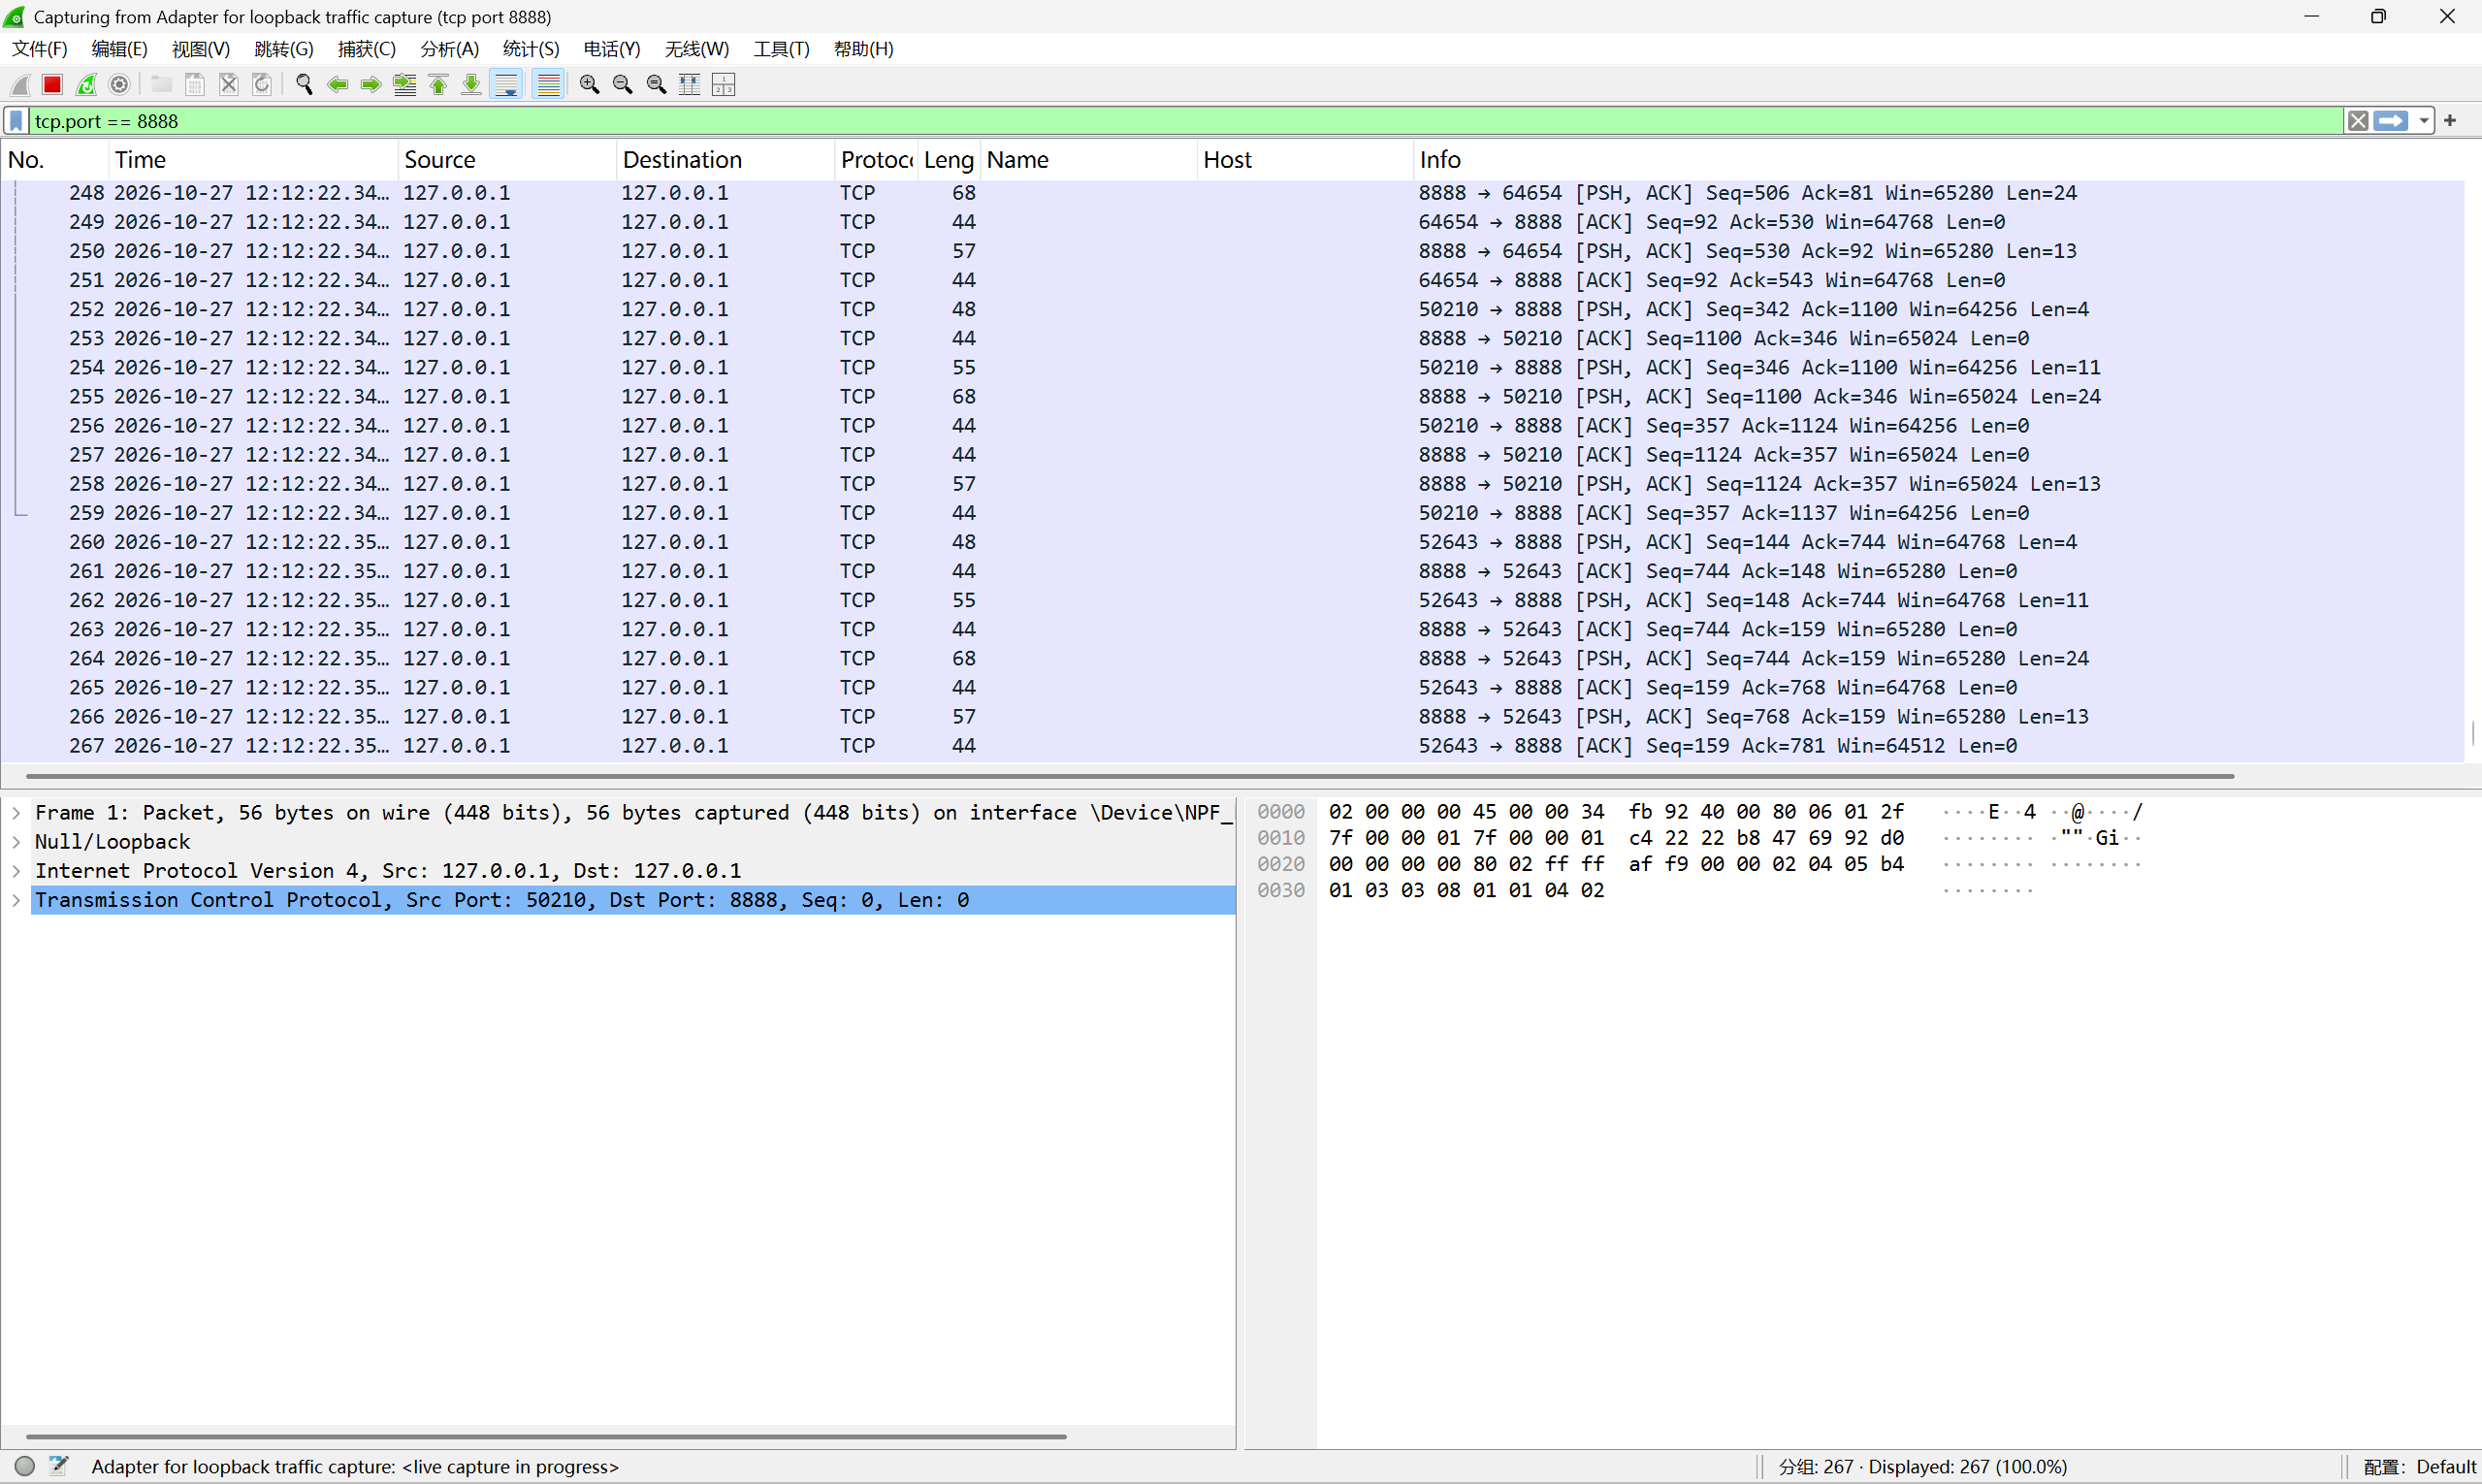
\includegraphics[width=\linewidth,height=10.0cm,keepaspectratio]{images/screen_79.png}
\captionof{figure}{退群对应的 TCP 流量}\label{fig:s79}
\par\smallskip{\raggedright\setlength{\parindent}{2em}\indent 列表中新增退群控制消息和成员通知，捕获保持运行。\par}
\end{minipage}\par\smallskip
\subsection{重连过程}
Charlie 断开后显示离线，此时列表累计 295 个分组；使用原昵称重新连接后，在线人数恢复为 3，抓包列表累计到 339 个分组。

\par\smallskip\noindent\begin{minipage}{\linewidth}\centering
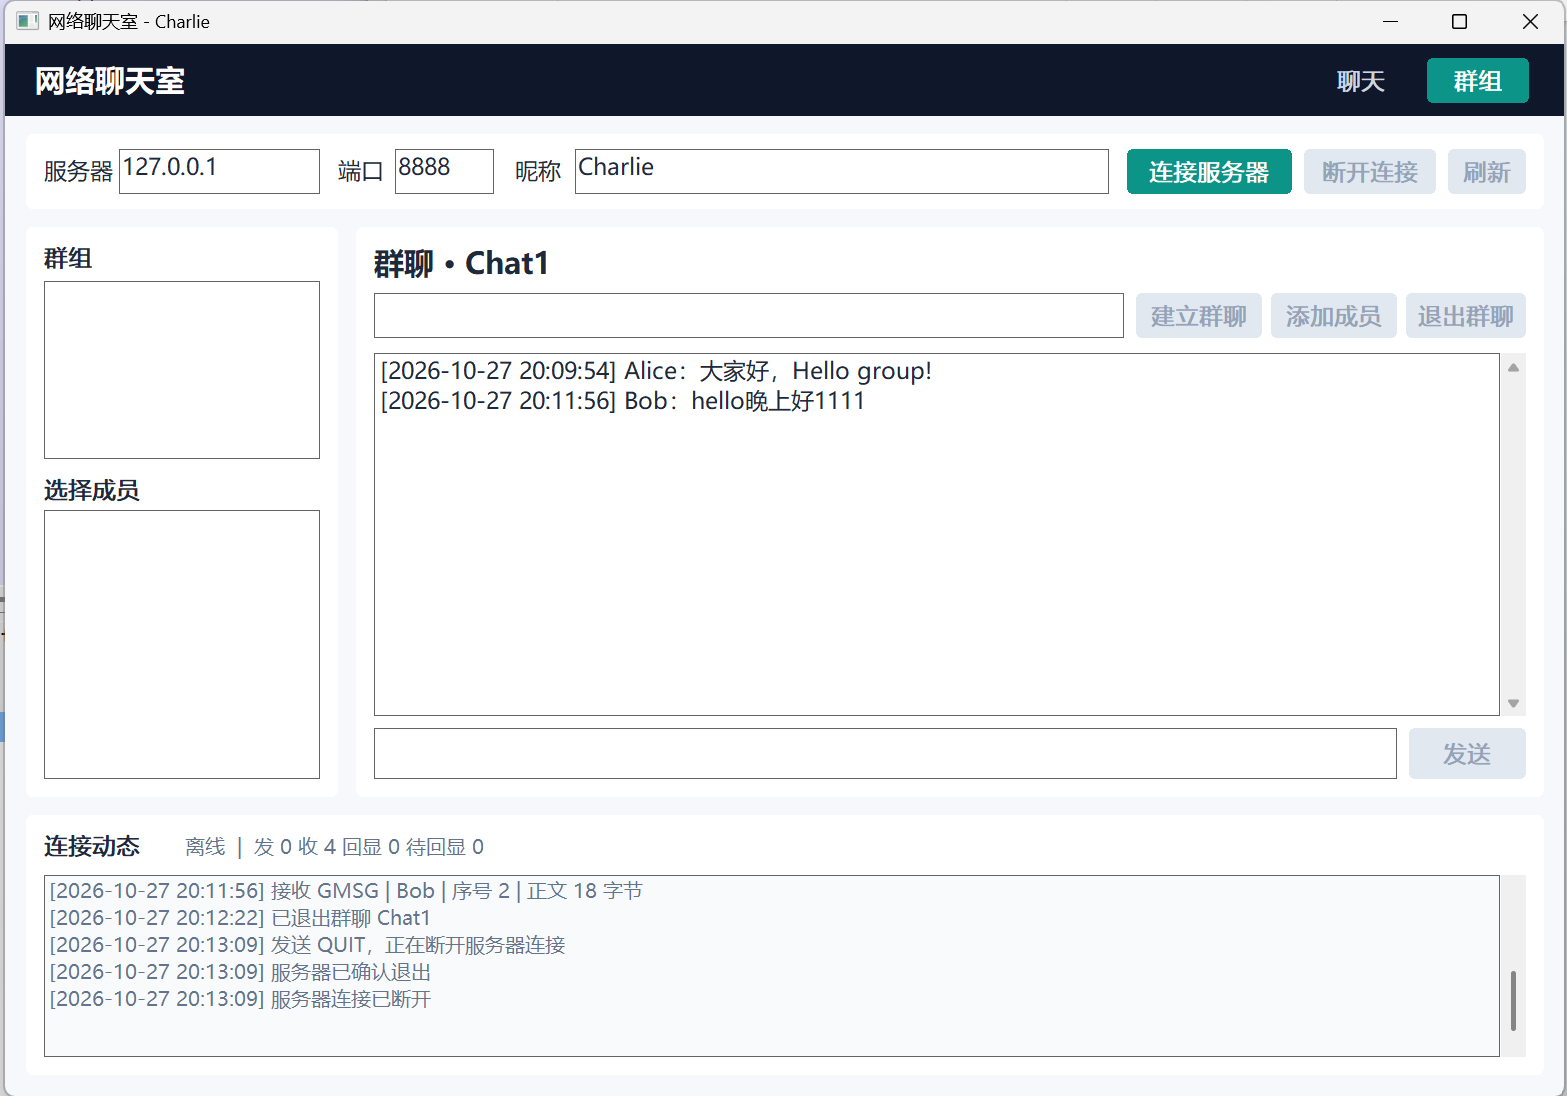
\includegraphics[width=\linewidth,height=10.0cm,keepaspectratio]{images/screen_80.png}
\captionof{figure}{抓包期间 Charlie 断开}\label{fig:s80}
\par\smallskip{\raggedright\setlength{\parindent}{2em}\indent Charlie 点击断开后显示退出确认及离线状态，接下来进入 TCP 释放过程。\par}
\end{minipage}\par\smallskip
\par\smallskip\noindent\begin{minipage}{\linewidth}\centering
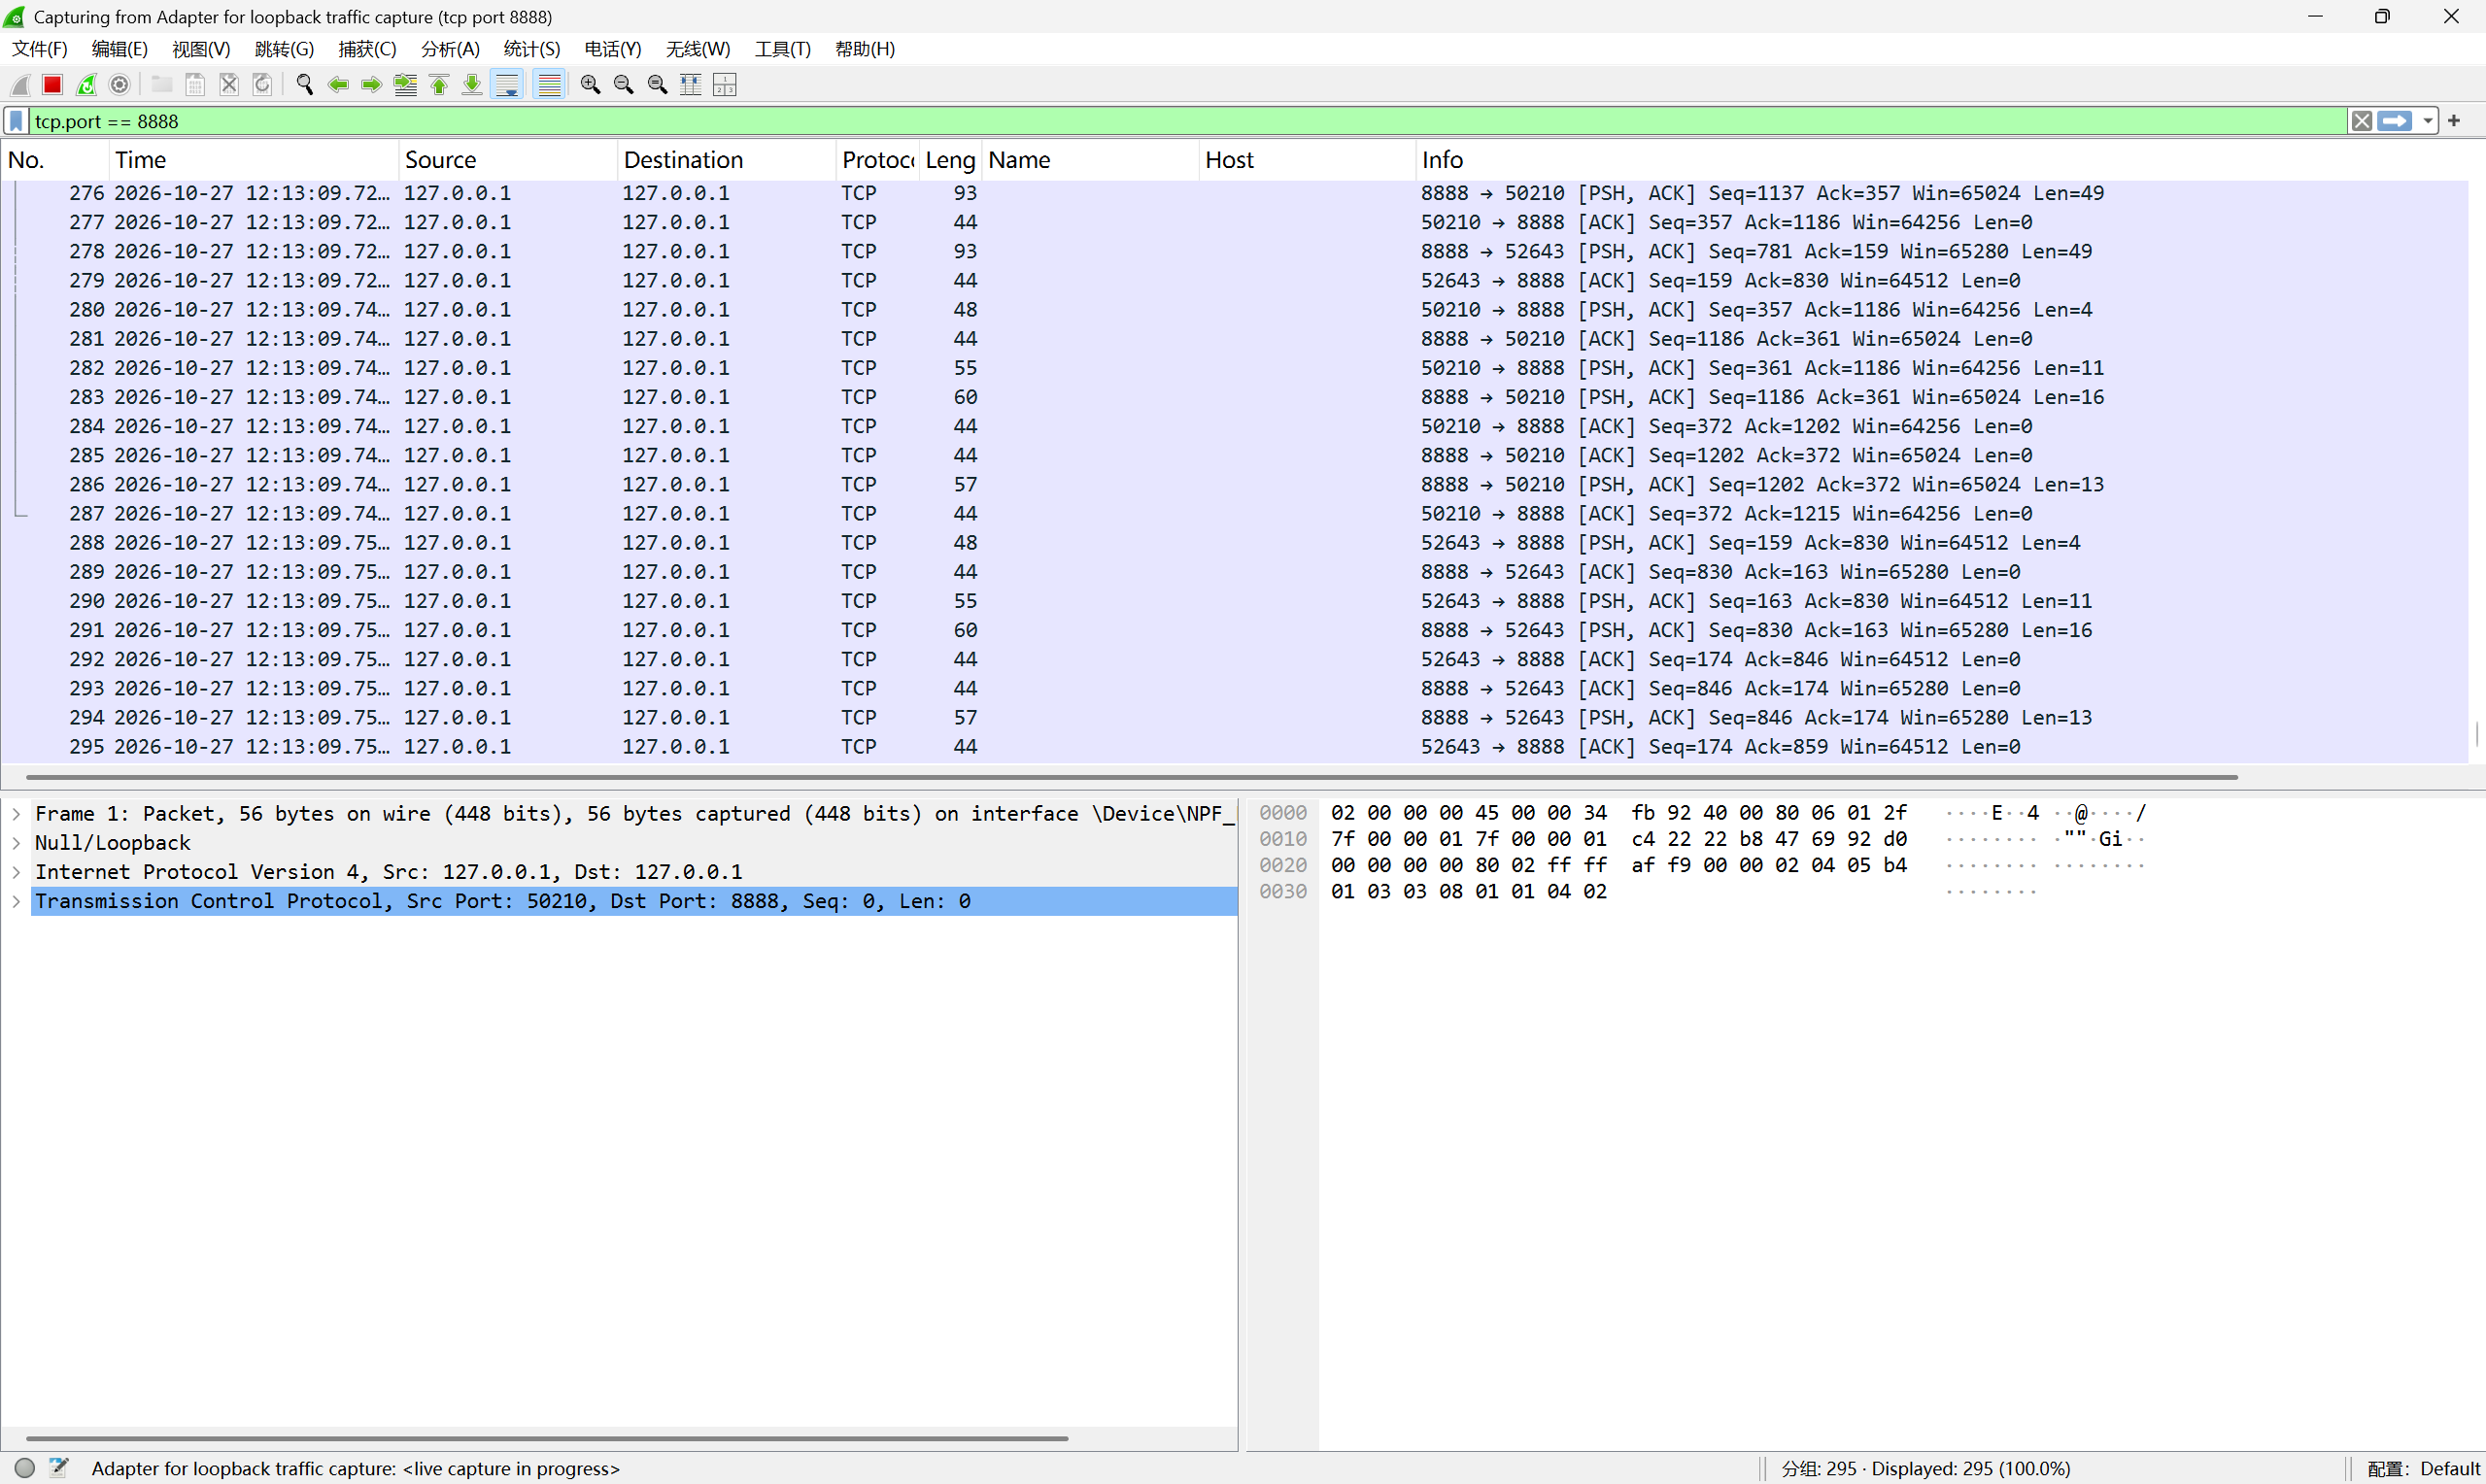
\includegraphics[width=\linewidth,height=10.0cm,keepaspectratio]{images/screen_81.png}
\captionof{figure}{Charlie 断开后的 TCP 流量}\label{fig:s81}
\par\smallskip{\raggedright\setlength{\parindent}{2em}\indent 这时列表累计 295 个分组，完整文件中的 QUIT、BYE、FIN 和 ACK 共同呈现该连接的退出。\par}
\end{minipage}\par\smallskip
\par\smallskip\noindent\begin{minipage}{\linewidth}\centering
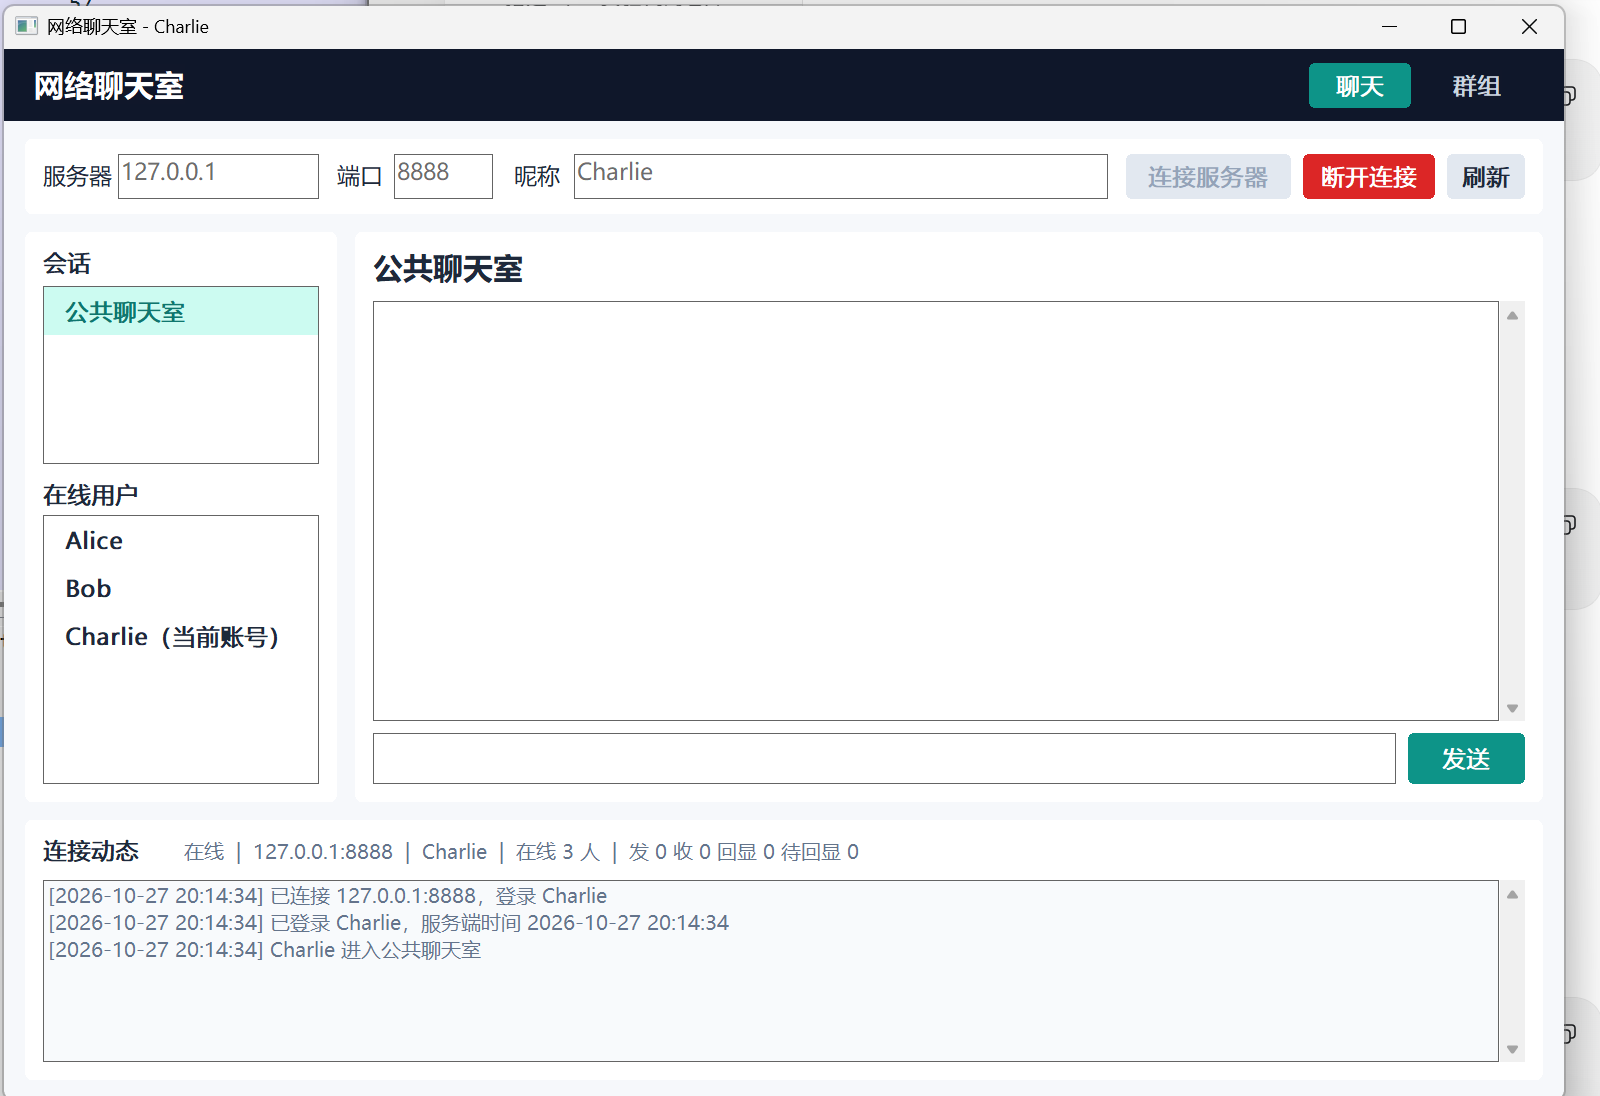
\includegraphics[width=\linewidth,height=10.0cm,keepaspectratio]{images/screen_82.png}
\captionof{figure}{抓包期间 Charlie 重连}\label{fig:s82}
\par\smallskip{\raggedright\setlength{\parindent}{2em}\indent Charlie 用原昵称重新连接，在线人数恢复为 3。\par}
\end{minipage}\par\smallskip
\par\smallskip\noindent\begin{minipage}{\linewidth}\centering
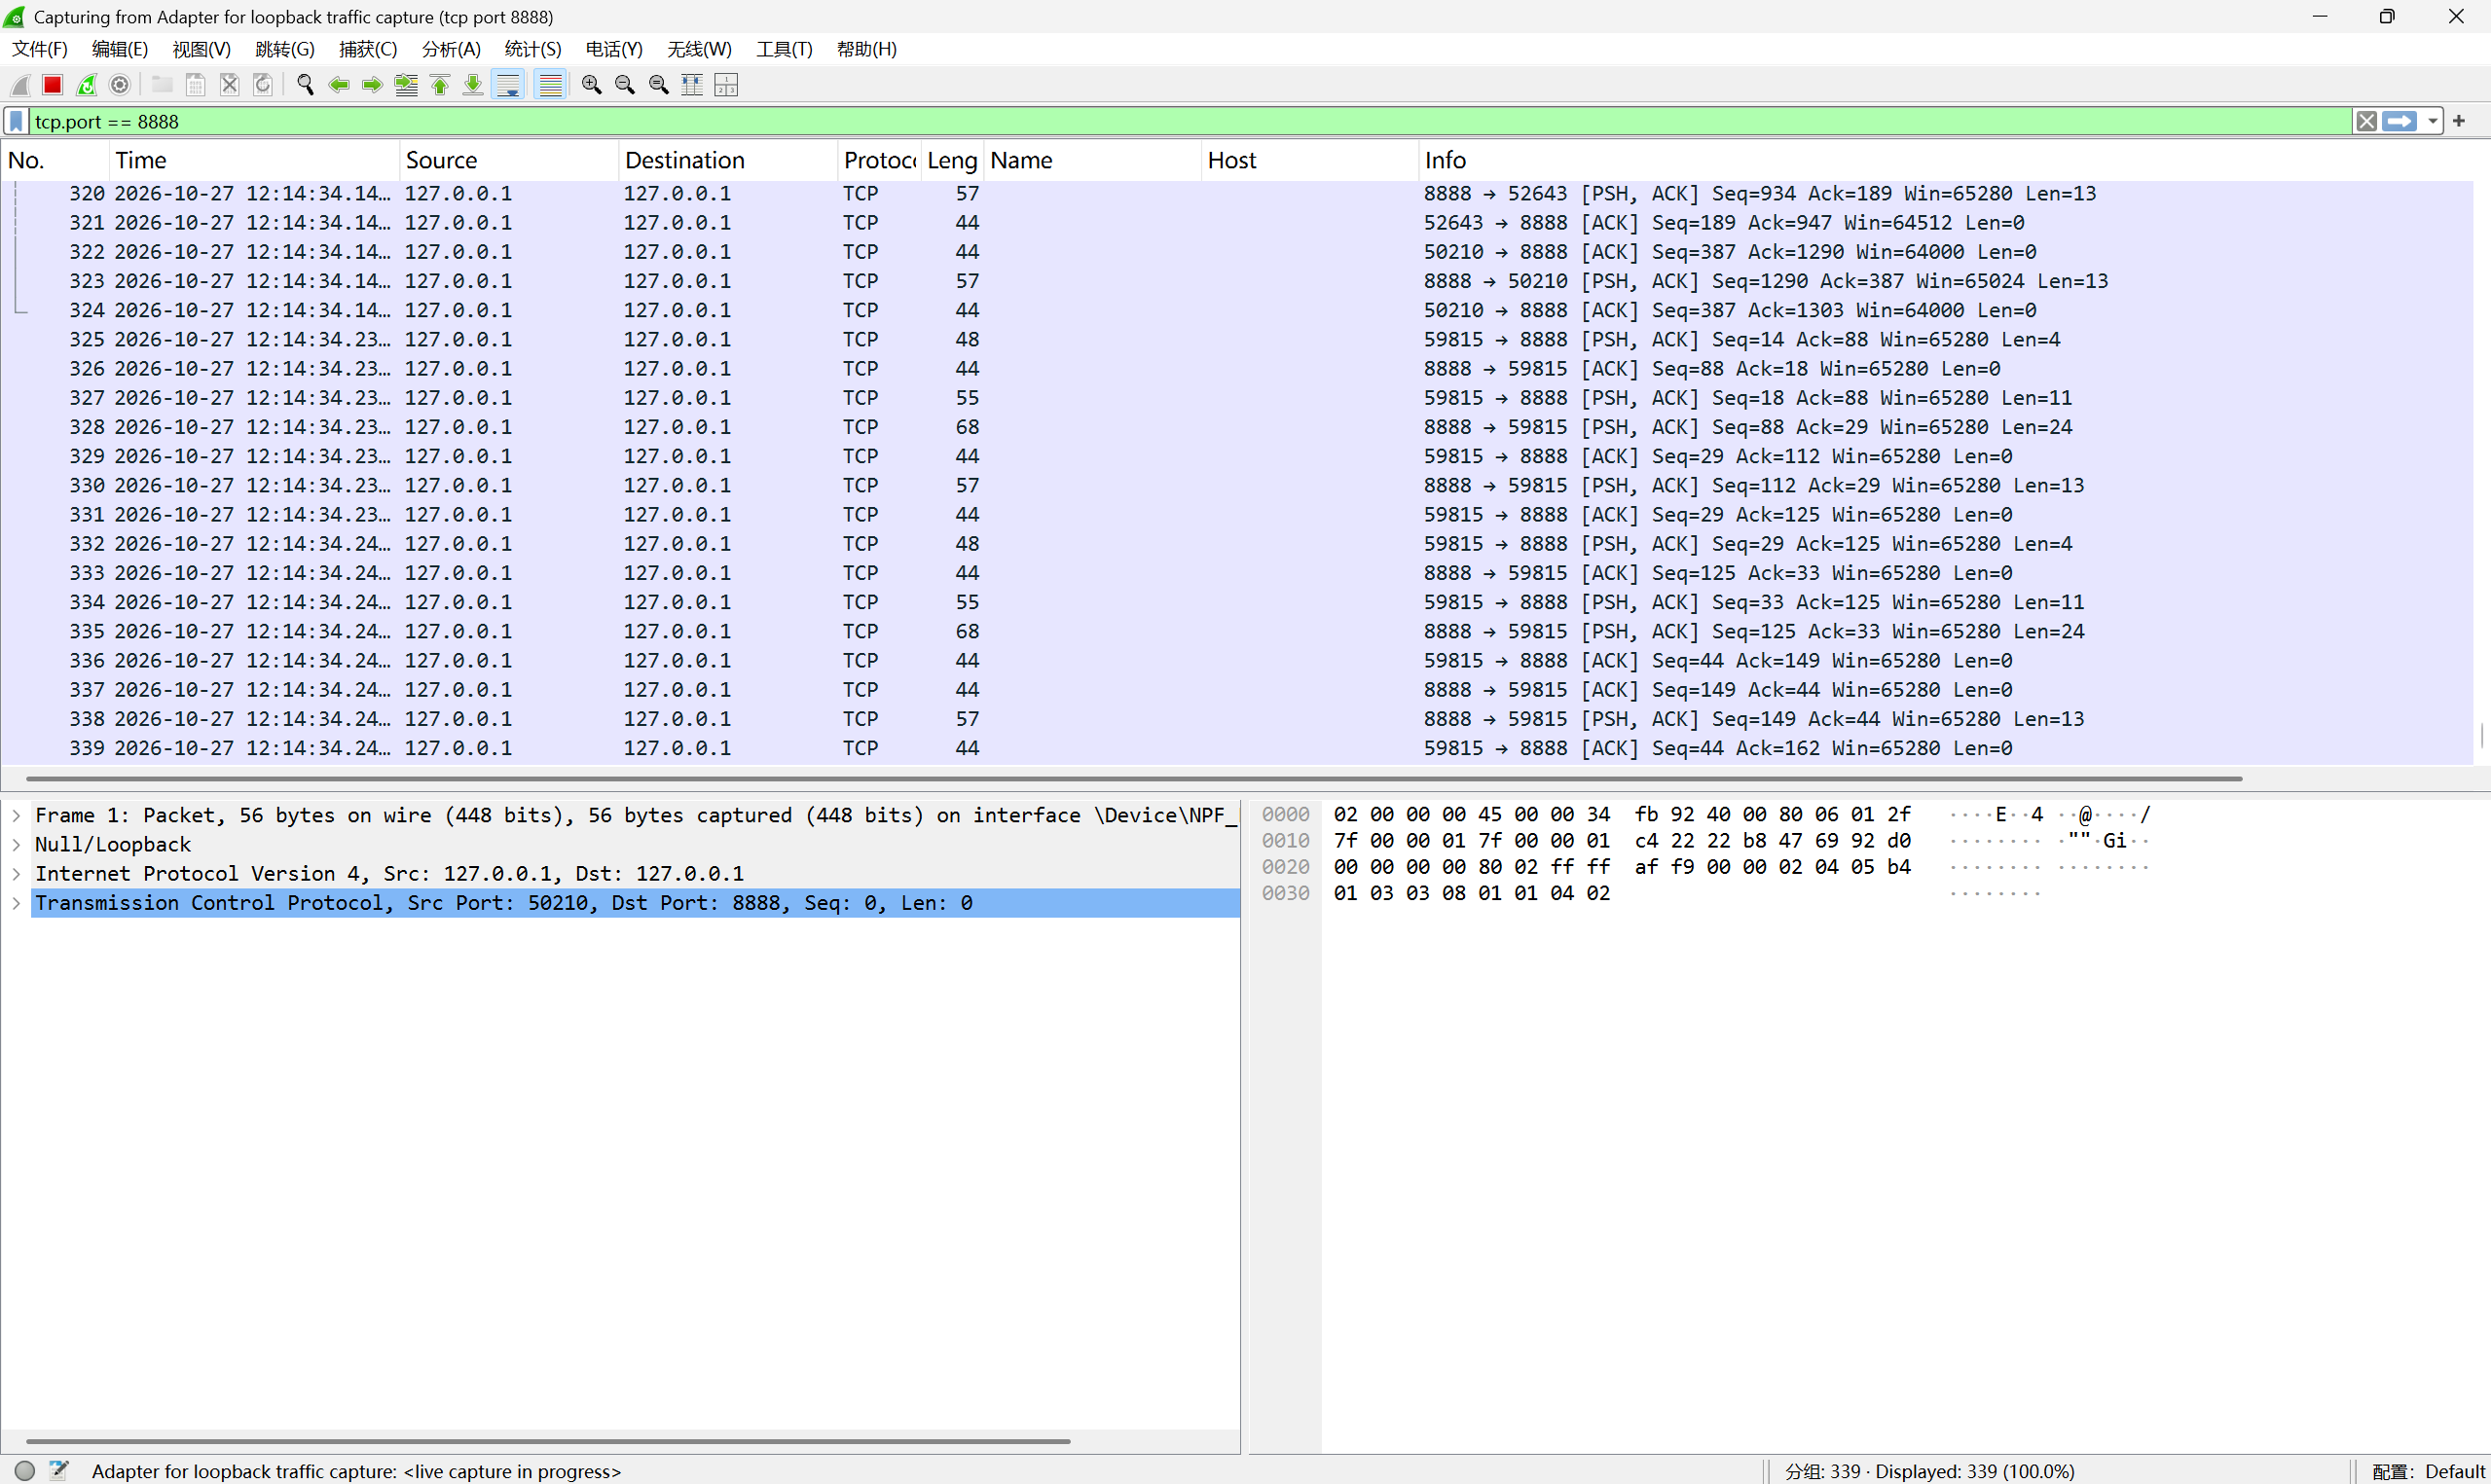
\includegraphics[width=\linewidth,height=10.0cm,keepaspectratio]{images/screen_83.png}
\captionof{figure}{Charlie 重连后的 TCP 流量}\label{fig:s83}
\par\smallskip{\raggedright\setlength{\parindent}{2em}\indent 重连后列表累计到 339 个分组，新临时端口对应新的流编号，其中还包含重新发送的 JOIN。\par}
\end{minipage}\par\smallskip
重新连接后，临时端口由 64654 变为 59815，流编号由 2 变为 3，说明建立了新的 TCP 会话。第 299 帧出现新的 JOIN，聊天序号也从新会话的 1 开始。

\subsection{重连后发送}
Charlie 重连后输入“我回来了！”，收到本人回显，待回显数为 0，第 340 帧对应 TEXT|\allowbreak{}1，三位在线用户都处于该公共消息的转发范围。随后关闭窗口，继续记录最后一次释放。

\par\smallskip\noindent\begin{minipage}{\linewidth}\centering
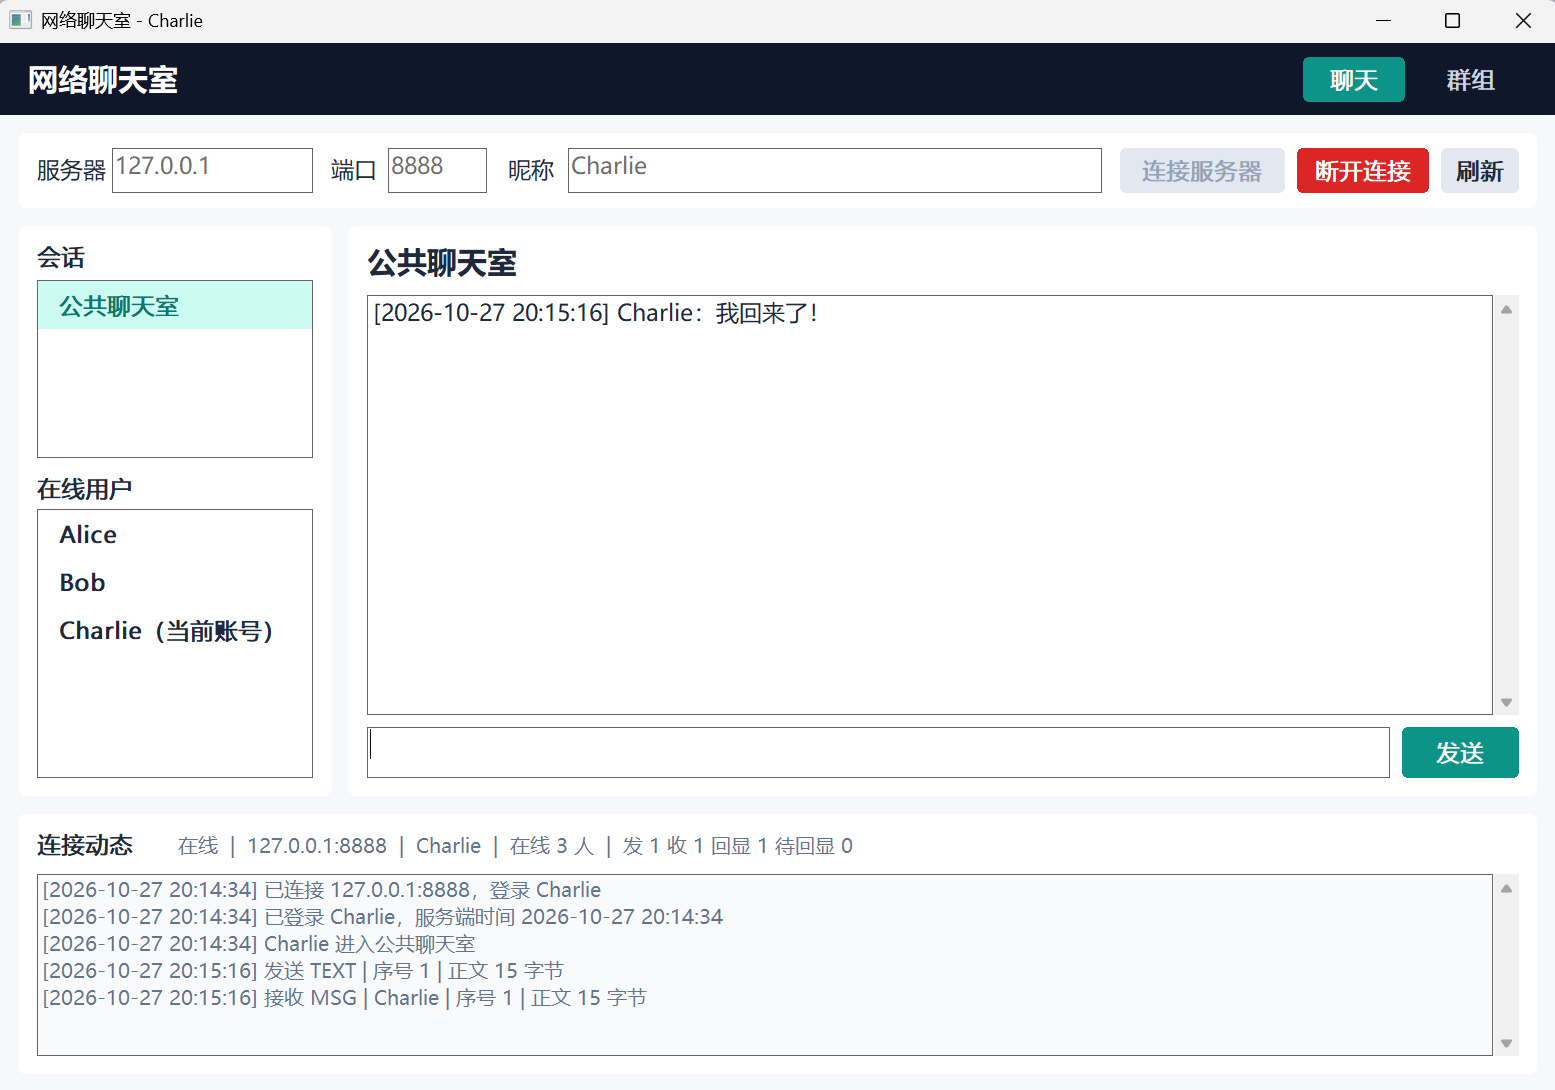
\includegraphics[width=\linewidth,height=10.0cm,keepaspectratio]{images/screen_84.png}
\captionof{figure}{Charlie 重连后的发言}\label{fig:s84}
\par\smallskip{\raggedright\setlength{\parindent}{2em}\indent Charlie 输入“我回来了！”后收到回显，待回显数为 0，显示新会话中的聊天已经完成。\par}
\end{minipage}\par\smallskip
\par\smallskip\noindent\begin{minipage}{\linewidth}\centering
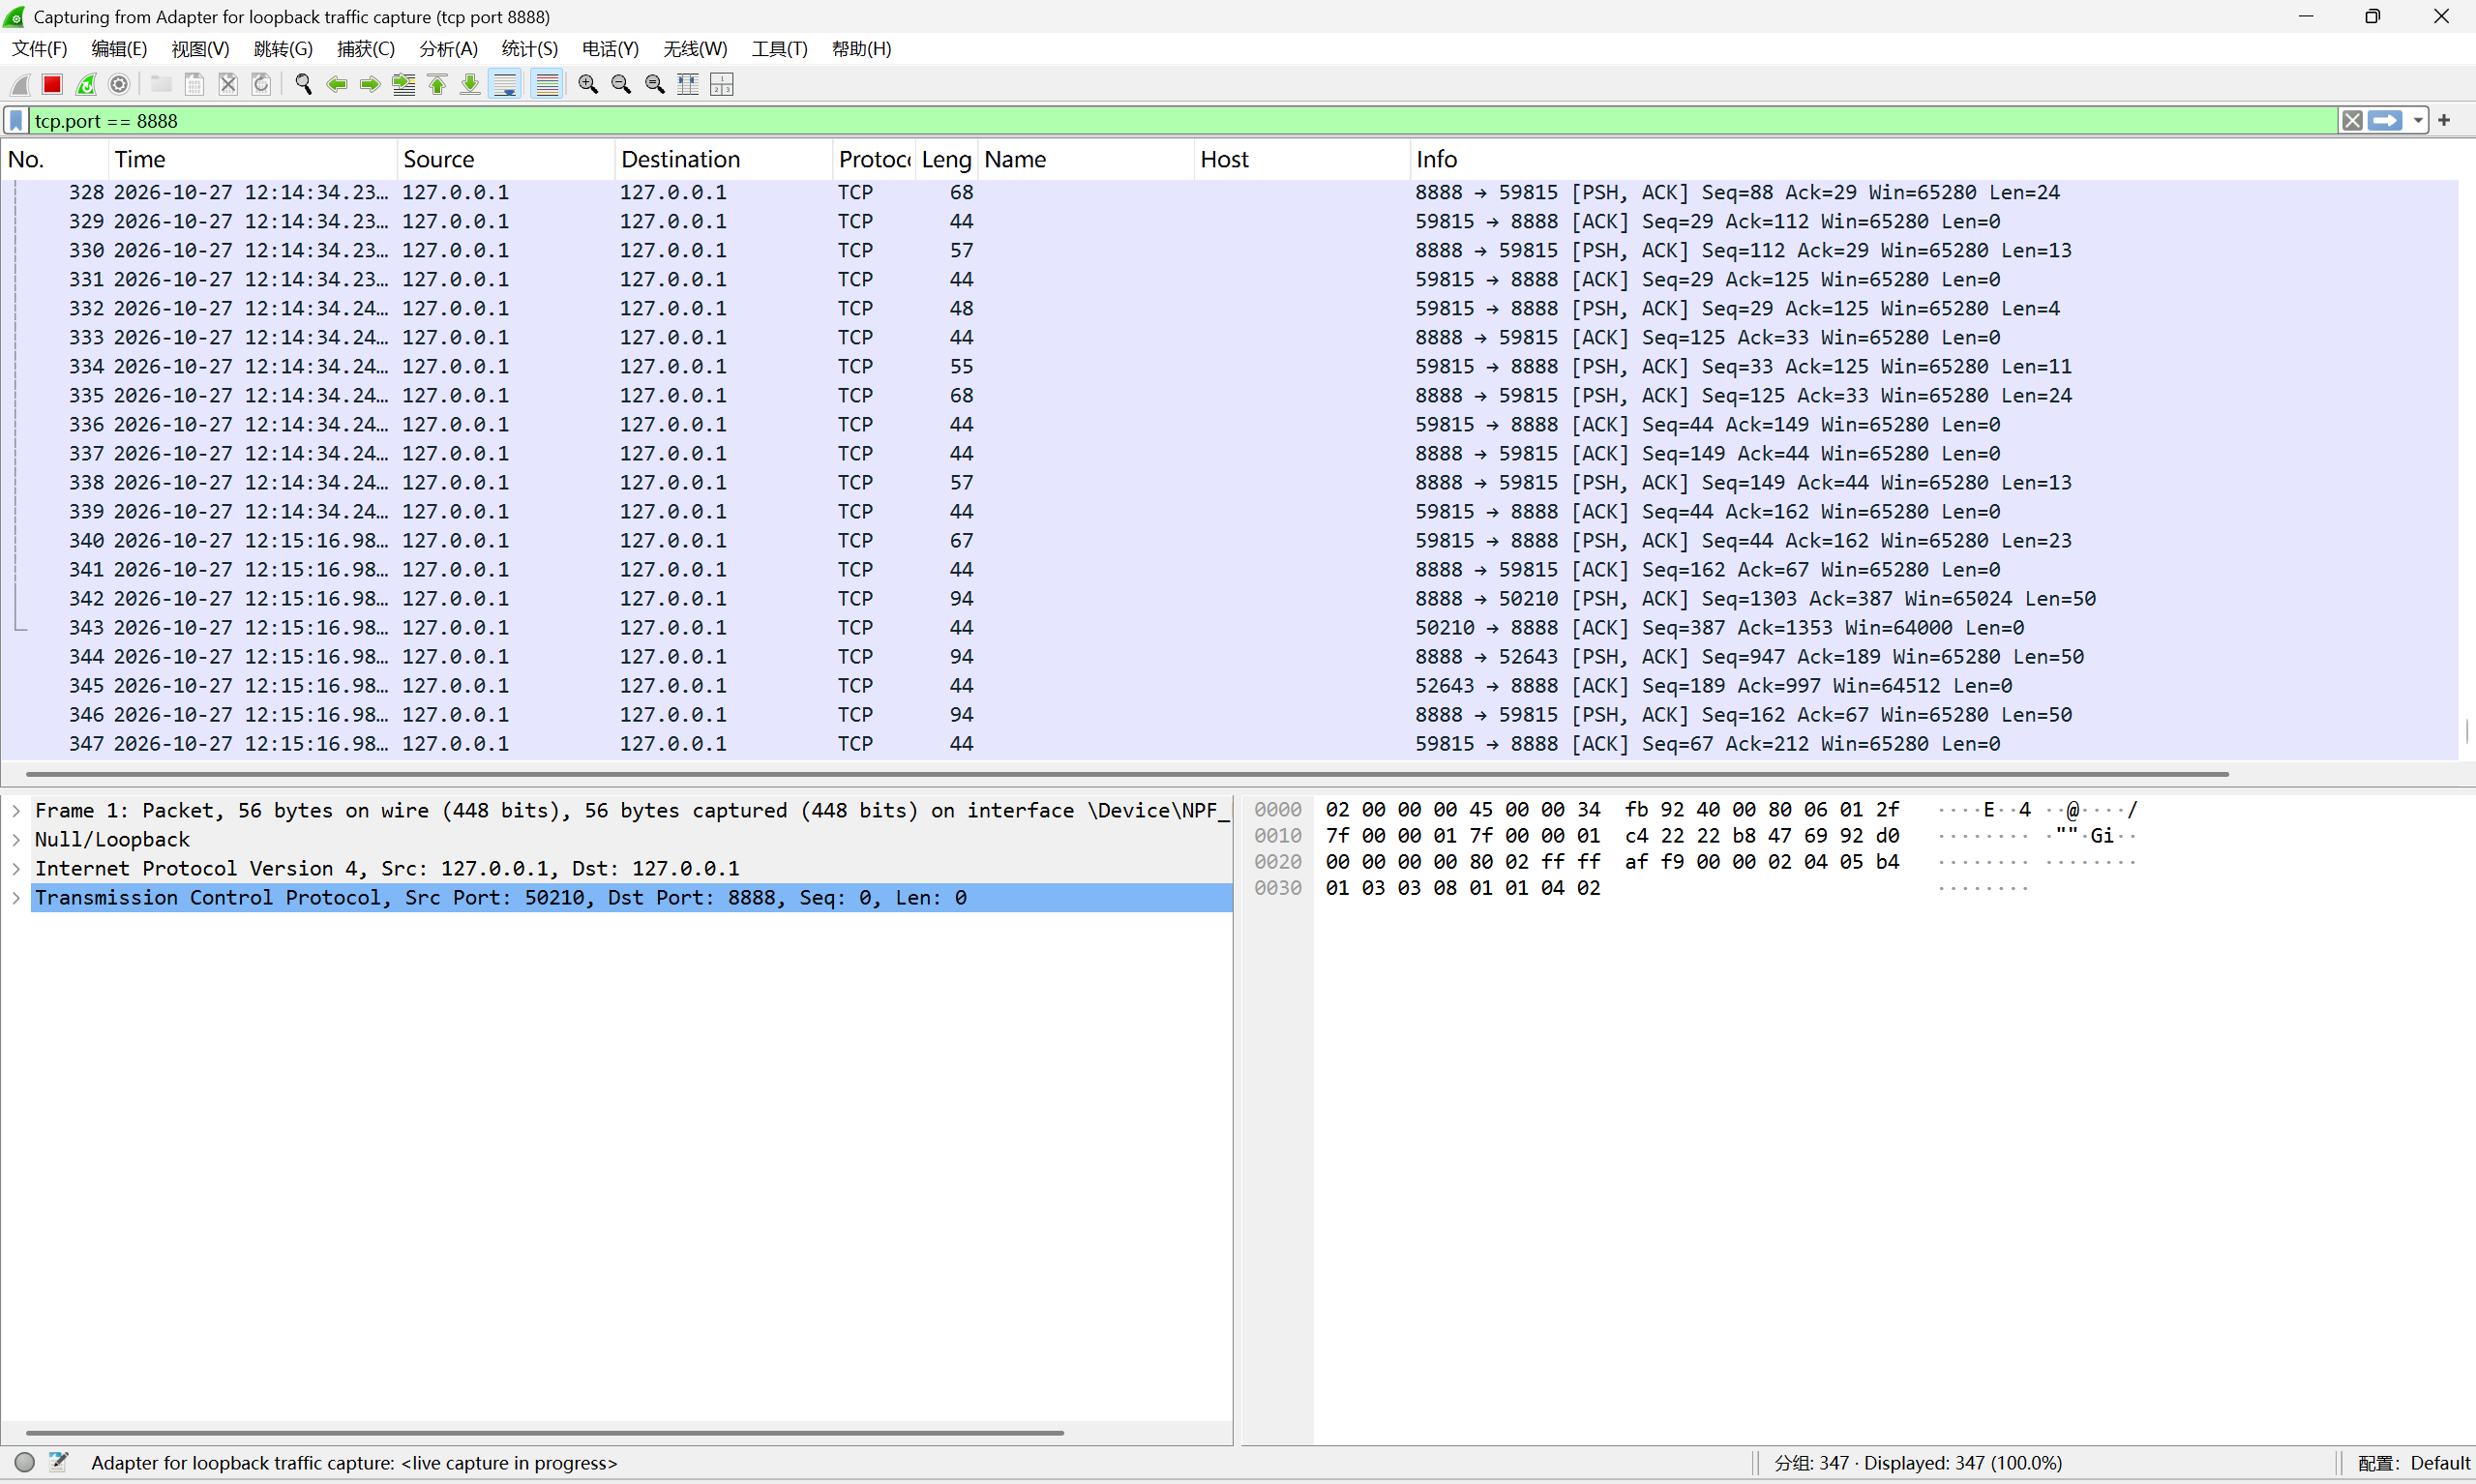
\includegraphics[width=\linewidth,height=10.0cm,keepaspectratio]{images/screen_85.png}
\captionof{figure}{重连后发言对应的 TCP 流量}\label{fig:s85}
\par\smallskip{\raggedright\setlength{\parindent}{2em}\indent 随后新增流量中可以找到 TEXT|\allowbreak{}1 及对应 MSG，应用序号已随新连接重新开始。\par}
\end{minipage}\par\smallskip
\par\smallskip\noindent\begin{minipage}{\linewidth}\centering
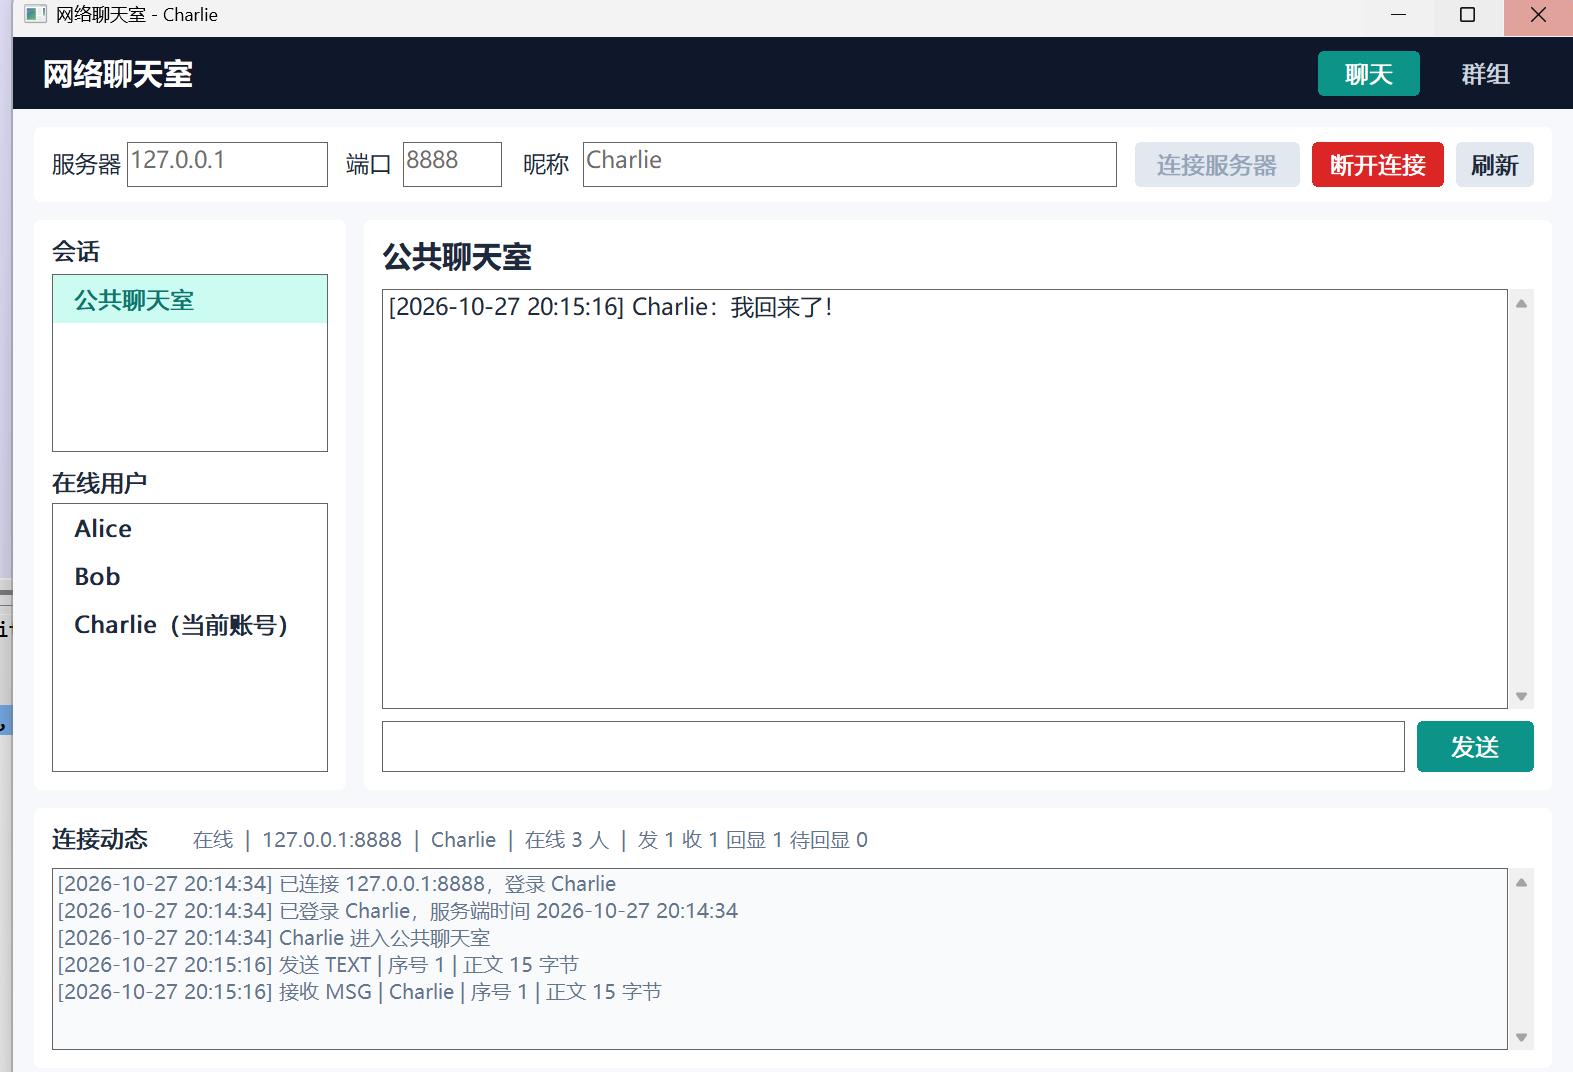
\includegraphics[width=\linewidth,height=10.0cm,keepaspectratio]{images/screen_86.png}
\captionof{figure}{Charlie 再次关闭前的状态}\label{fig:s86}
\par\smallskip{\raggedright\setlength{\parindent}{2em}\indent 再次关闭窗口前，Charlie 仍显示在线，并已收到最后一条发言的本人回显。\par}
\end{minipage}\par\smallskip
\par\smallskip\noindent\begin{minipage}{\linewidth}\centering
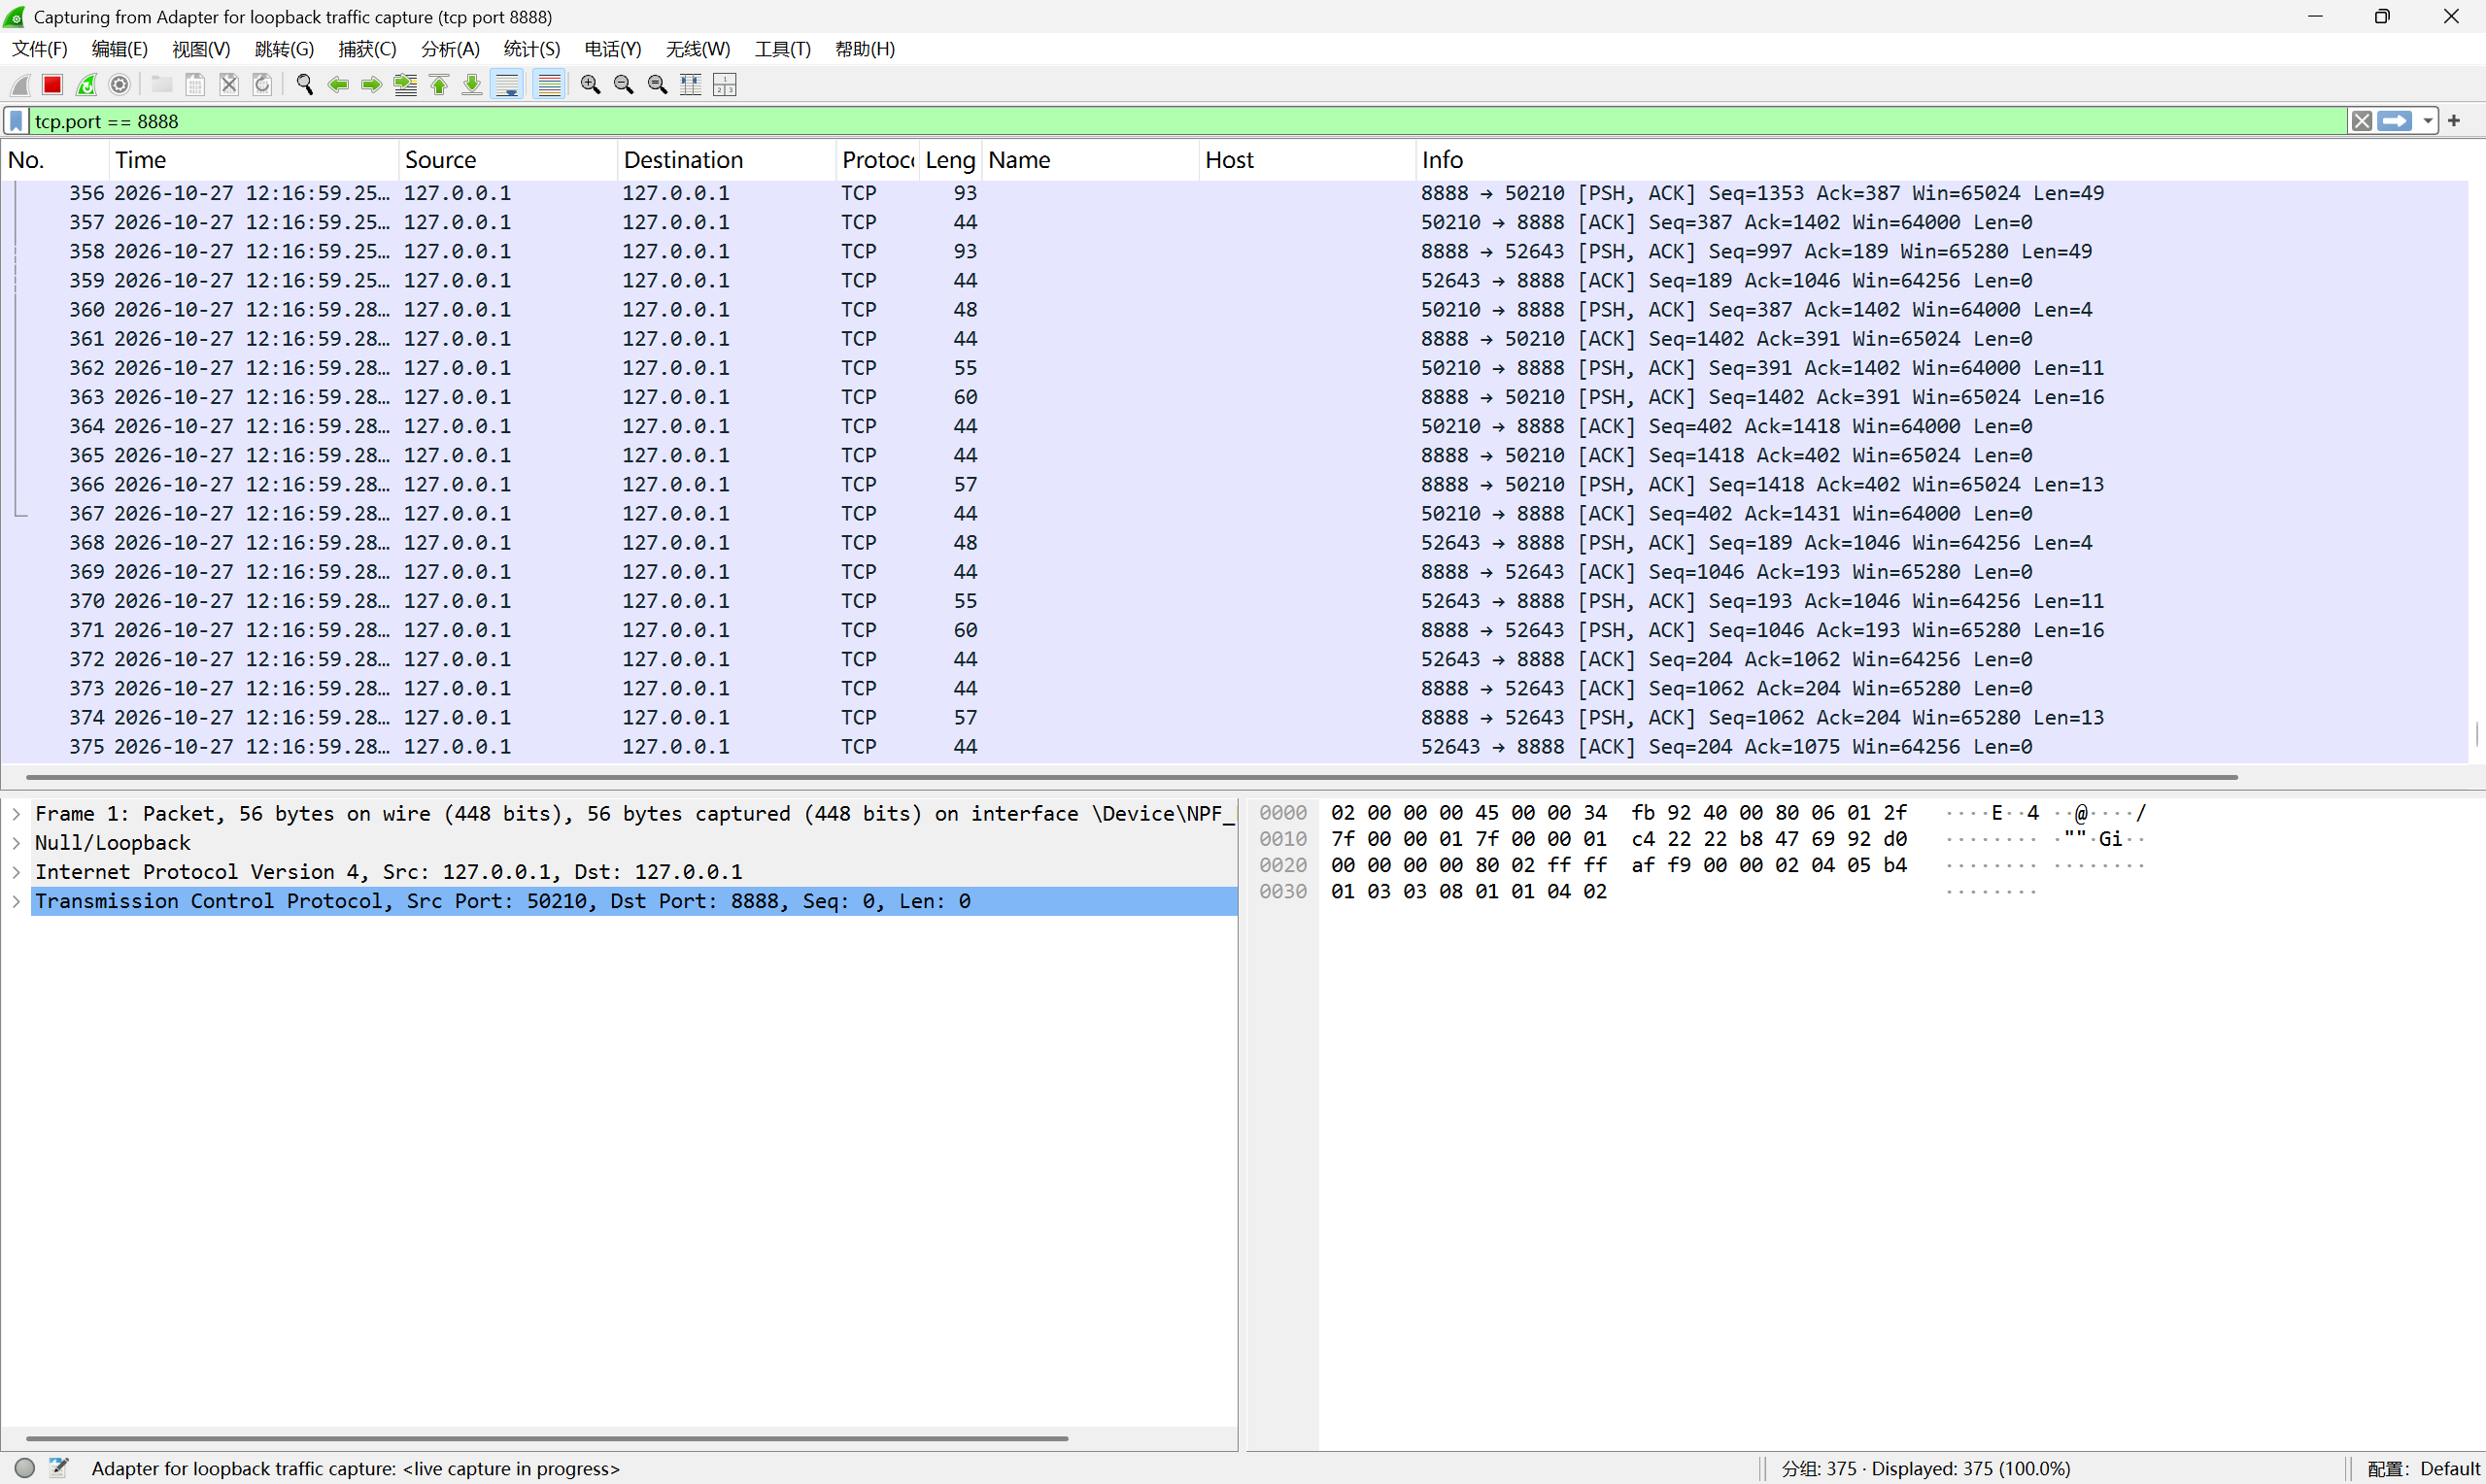
\includegraphics[width=\linewidth,height=10.0cm,keepaspectratio]{images/screen_87.png}
\captionof{figure}{关闭 Charlie 后保存的抓包}\label{fig:s87}
\par\smallskip{\raggedright\setlength{\parindent}{2em}\indent 关闭窗口并停止捕获后，保存文件包含 375 帧，最后一次连接释放也保存在其中。\par}
\end{minipage}\par\smallskip
停止捕获后保存了包含 375 帧的文件，前面的截图呈现捕获过程中逐渐增加的列表，后面的帧号、正文和统计则来自这份完整文件。

\subsection{三次握手}
\par\medskip\noindent\begin{minipage}{\linewidth}\centering
\begin{tabular}{@{}>{\raggedright\arraybackslash}p{0.113\linewidth}>{\raggedright\arraybackslash}p{0.281\linewidth}>{\raggedright\arraybackslash}p{0.544\linewidth}@{}}
\toprule
帧号 & 方向 & 标志和相对序号\\
\midrule
1 & 50210 -> 8888 & SYN；Seq=0\\
2 & 8888 -> 50210 & SYN, ACK；Seq=0，Ack=1\\
3 & 50210 -> 8888 & ACK；Seq=1，Ack=1\\
\bottomrule
\end{tabular}
\captionof{table}{Alice 首次连接的三次握手}
\end{minipage}\par\medskip
Alice 的首次连接依次出现第 1 帧 SYN、第 2 帧 SYN、ACK 和第 3 帧 ACK，完成三次握手后才在第 4 帧发送 JOIN|\allowbreak{}Alice。Wireshark 使用相对序号，SYN 占用一个序号，因此后续从 Seq=1 开始。[3][5]

Charlie 重连时，第 296、297、298 帧再次出现同样的三步交互，结合新端口和流编号，可以区分旧连接释放与新连接建立。

\subsection{连接释放}
\par\medskip\noindent\begin{minipage}{\linewidth}\centering
\begin{tabular}{@{}>{\raggedright\arraybackslash}p{0.113\linewidth}>{\raggedright\arraybackslash}p{0.281\linewidth}>{\raggedright\arraybackslash}p{0.544\linewidth}@{}}
\toprule
帧号 & 方向 & 内容或标志\\
\midrule
268 & 64654 -> 8888 & QUIT 应用请求\\
270 & 64654 -> 8888 & FIN, ACK；客户端关闭发送方向\\
271 & 8888 -> 64654 & BYE 应用响应\\
274 & 8888 -> 64654 & FIN, ACK；服务器关闭发送方向\\
275 & 64654 -> 8888 & ACK；确认服务器 FIN\\
\bottomrule
\end{tabular}
\captionof{table}{Charlie 主动断开的关键帧}
\end{minipage}\par\medskip
应用退出通过 QUIT、BYE 完成，传输层关闭则通过 FIN、ACK 完成。客户端发送 QUIT 后关闭写方向，但继续读取 BYE，随后双方分别结束发送方向，形成表中的释放过程。

最后关闭窗口时，第 348 帧为 QUIT，第 350 帧为客户端 FIN，第 352 帧为 BYE，第 354 帧为服务器 FIN，第 355 帧为最终 ACK；两次 Charlie 退出共出现 4 个 FIN，分别属于两条连接的双向关闭。

\subsection{应用消息交付}
按 TCP 流及方向重组负载、以 LF 提取完整帧后，得到 180 条应用消息，其中包含登录、名单、通知、群控制及退出，聊天请求为 6 条。根据公聊、私聊及群聊的转发范围，可以得到下表中的预期接收者。

\par\medskip\noindent\begin{minipage}{\linewidth}\centering
\begin{tabular}{@{}>{\raggedright\arraybackslash}p{0.118\linewidth}>{\raggedright\arraybackslash}p{0.292\linewidth}>{\raggedright\arraybackslash}p{0.364\linewidth}>{\raggedright\arraybackslash}p{0.137\linewidth}@{}}
\toprule
请求帧 & 类型和发送者 & 预期接收者 & 转发次数\\
\midrule
103 & Alice 公聊 & Alice、Bob、Charlie & 3\\
111 & Alice 私聊 Bob & Alice、Bob & 2\\
213 & Alice 向 Chat1 群发 & Alice、Bob、Charlie & 3\\
221 & Bob 公聊 & Alice、Bob、Charlie & 3\\
229 & Bob 向 Chat1 群发 & Alice、Bob、Charlie & 3\\
340 & Charlie 重连后公聊 & Alice、Bob、Charlie & 3\\
\bottomrule
\end{tabular}
\captionof{table}{聊天请求的转发结果}
\end{minipage}\par\medskip
\[
N_{\mathrm{forward}}=3+2+3+3+3+3=17
\]
以发送者、应用序号、类型、群名或目标及正文匹配后，17 次预期交付都能在相应接收流中找到，缺失和额外项均为 0。这里统计手动演示的六条请求，自动化负载测试的 900 次交付则来自另一组日志。

\Needspace{7\baselineskip}
\subsection{重传观察}
\Needspace{4\baselineskip}
\VerbatimInput[fontsize=\small,breaklines=true,breakanywhere=true,numbers=left,firstnumber=1,numbersep=6pt,tabsize=4,baselinestretch=1.05]{code/listing_40.txt}
\medskip
\Needspace{4\baselineskip}
\VerbatimInput[fontsize=\small,breaklines=true,breakanywhere=true,numbers=left,firstnumber=1,numbersep=6pt,tabsize=4,baselinestretch=1.05]{code/listing_41.txt}
\medskip
\begin{longtable}{@{}>{\raggedright\arraybackslash}p{0.598\linewidth}>{\raggedright\arraybackslash}p{0.367\linewidth}@{}}
\toprule
指标 & 结果\\
\midrule\endfirsthead
\toprule
指标 & 结果\\
\midrule\endhead
TCP 分组总数 & 375\\
TCP 流数量 & 4\\
SYN / SYN ACK & 4 / 4\\
FIN / RST & 4 / 0\\
重传分析标记 & 0\\
前序分段未捕获标记 & 0\\
重复 ACK 标记 & 0\\
捕获接口接收数 & 375\\
捕获接口丢弃数 & 0\\
聊天请求 & 6\\
预期转发 / 实际匹配 & 17 / 17\\*
\bottomrule
\caption{完整演示抓包统计}\\
\end{longtable}
对保存流量应用重传、前序分段未捕获和重复 ACK 过滤器，结果都为 0，接口丢弃数也为 0；结合重组正文，可以看到聊天请求均有对应转发。

TCP 分析标记来自序列号及确认状态，描述的是传输过程，界面的发送数、回显数描述的则是应用请求。理解两类计数的层次后，才能解释网络重传或待回显记录等现象。[6]

抓包截图使用 UTC，聊天时间采用北京时间，两者相差 8 小时，因此将时间统一后，再结合端口、流编号和正文，可以对应到同一操作。

\Needspace{10\baselineskip}
\section{问题分析}
\subsection{消息边界}
TCP 接收按字节推进，中文编码可能跨多批到达，多条消息也可能一起读入，因此采用“缓存字节、按 LF 分帧、解析完整正文”的顺序处理。拆分发送后仍收到完整中文，合并发送后得到两条独立正文，呈现了这一处理的实际效果。

分帧确定应用消息边界，TCP 确认及重传提供字节传输可靠性，二者分属不同层次。采用统一帧格式后，业务函数收到的是完整消息，界面也能按会话连续保存正文。

\subsection{退群后的计数}
Charlie 退群后发送得到 NOT\_MEMBER，但待回显数仍为 1。对应源码中，发送时已将序号加入 awaiting\_echo，ERR 分支却只追加错误文本，原等待项仍保留，所以重新入群后虽然可以正常聊天，之前的计数仍留在界面上。

这个问题位于失败请求的收尾处理：可以在错误响应中返回请求序号，按序号移除对应等待项，再在连接结束时清理剩余记录。这样成功回显和失败响应都拥有明确结束状态，显示计数才能随实际处理结果变化。

\Needspace{4\baselineskip}
\VerbatimInput[fontsize=\small,breaklines=true,breakanywhere=true,numbers=left,firstnumber=1,numbersep=6pt,tabsize=4,baselinestretch=1.05]{code/listing_42.txt}
\medskip
\subsection{脚本编码}
启动脚本曾在 Windows PowerShell 中提示缺少右花括号，源文件中的语句结构完整，问题出在中文脚本的编码读取。将文件保存为带 BOM 的 UTF-8 后，同样的启动语句可以正常解析，服务器和三个客户端也能够打开。

另外，将工程根目录设为启动进程的工作目录，并按可执行文件位置找到 evidence，可以在从其他目录调用脚本时继续读取资源、保存日志。

\subsection{界面布局}
早期缩小窗口时，连接参数和按钮出现重叠，随后将位置计算集中到 layout\_controls，根据客户区宽高重新布局，并按 DPI 调整字体及间距。横向和纵向调整后的截图中，输入框、发送按钮和动态区都保持可见。

聊天正文放在上方会话区，上下线和成员提示放在底部，切换私聊或群聊时只改变对应历史，连接事件继续按时间追加，因此两类内容在界面上保持清楚的层次。

\Needspace{10\baselineskip}
\section{实验总结}
通过这个实验，我完成了采用 C/S 架构的 TCP 聊天室，实现了中英文公聊、私聊和群聊，并在消息中加入服务器时间。经过测试，三个客户端能够同时收发消息，私聊和群聊的转发范围符合设计，断开后可以使用原昵称重新登录。通过 Wireshark 抓包，可以看到连接建立、数据传输和连接释放的完整过程。

在实验中我也遇到了一些问题。设计协议时，需要区分字段分隔符和正文中的竖线。我根据消息类型拆分前面的固定字段，将剩余内容整体作为正文，保留其中的竖线。在编写收发代码时，需要处理一条消息分多次到达、多条消息同时到达，以及多个线程同时发送的情况。我使用缓存累计接收字节，按换行符提取完整消息，并为每条连接设置发送锁，保证各线程完整发送一条消息后再交替处理。

通过实验，我学会了使用 C++ 和基本 Socket 函数编写基于 TCP 的多用户聊天室，完成了协议设计、服务器和客户端的实现及功能测试，也更深刻地了解了消息分帧、多线程同步和连接管理的作用；在测试时，我也学会了借助 Wireshark 观察实际通信，辅助分析消息传输和连接状态。

\Needspace{10\baselineskip}
\section{参考文献}
[1] 编程实验1 利用流式套接字编写聊天程序．实验要求、评分标准、实验报告要求．课堂幻灯片，2026年10月14日。

[2] 计算机网络与信息安全研究室．计算机网络 第二章 应用层协议及网络编程．课程讲义，2023年，第24～46页。

[3] 计算机网络与信息安全研究室．计算机网络 第三章 传输层协议．课程讲义，2023年，第48～54页及TCP连接管理部分。

[4] Microsoft．Getting started with Winsock．Microsoft Learn．访问日期2026年10月29日。 \url{https://learn.microsoft.com/en-us/windows/win32/winsock/getting-started-with-winsock}

[5] Eddy W，编．RFC 9293 Transmission Control Protocol TCP．IETF，2022。 \url{https://www.rfc-editor.org/rfc/rfc9293.html}

[6] Wireshark Foundation．Wireshark User’s Guide 第7.5节 TCP Analysis．访问日期2026年10月29日。 \url{https://www.wireshark.org/docs/wsug_html_chunked/ChAdvTCPAnalysis.html}

\end{document}
